%%____________________________________________________________________________||

\newlength\cmsFigWidth
\ifthenelse{\boolean{cms@external}}{\setlength\cmsFigWidth{0.85\columnwidth}}{\setlength\cmsFigWidth{0.4\textwidth}}
\ifthenelse{\boolean{cms@external}}{\providecommand{\cmsLeft}{top\xspace}}{\providecommand{\cmsLeft}{left\xspace}}
\ifthenelse{\boolean{cms@external}}{\providecommand{\cmsRight}{bottom\xspace}}{\providecommand{\cmsRight}{right\xspace}}

%%____________________________________________________________________________||

\cmsNoteHeader{AN-17-122}

%%____________________________________________________________________________||

\title{Search for supersymmetry in pp collisions using final states
with at least one jet and missing transverse momentum}

%%____________________________________________________________________________||

\author[imperial]{R.~Bainbridge}
\author[bristol]{E.~Bhal}
\author[vub]{F.~Blekman}
\author[imperial]{S.~Breeze}
\author[imperial]{O.~Buchm\"uller}
\author[imperial]{S.~Casasso}
\author[imperial]{M.~Citron}
\author[imperial]{A.~Elwood}
\author[bristol]{H.~Fl\"acher}
\author[rochester]{A.~Garcia-Bellido}
\author[imperial]{C.~Laner}
\author[rochester]{K.H.~Lo}
\author[imperial]{S.A.~Malik}
\author[imperial]{B.~Penning}
\author[bristol]{T.~Sakuma}
\author[vub]{D.~Smith$^{1}$}
\author[imperial]{A.~Tapper}

\address[bristol]{University of Bristol, Bristol, UK}
\address[imperial]{Imperial College, London, UK}
\address[vub]{Vrije Universiteit Brussel, Brussel, BE}
\address[rochester]{University of Rochester, NY, US}

%%____________________________________________________________________________||

\date{\today}

%%____________________________________________________________________________||

\abstract{A search for supersymmetry is performed in final states
containing one or more jets and an imbalance in transverse momentum. A
sample of events resulting from pp collisions at a centre-of-mass
energy of 13\TeV is analysed. The event data were recorded with the
CMS detector at the CERN LHC in 2016 and correspond to an integrated
luminosity of 36.3\fbinv. The search provides sensitivity to models
that predict a stable weakly interacting massive particle, such as the
neutralino. The search employs several kinematic variables to suppress
multijet production to a subdominant level with respect to all other
standard model backgrounds. Several further kinematic variables are
used for signal extraction using a binned maximum-likelihood fit to
the data. The number of candidate signal events is found to agree with
the expected event counts from standard model processes. A number of
simplified supersymmetric models that assume the production of gluino
or squark pairs that decay to neutralinos and standard model
particles, are used to interpret the result. For models that assume
the production of gluino pairs, gluino and neutralino masses up to X
and Y\GeV, respectively, are excluded. For models that assume In the
case of the production of squark pairs, light-flavour, bottom, and top
squarks masses up to X, Y, and Z\GeV are excluded,
respectively. Models with near-degenerate mass spectra are also
considered. For models that assume top-squark production and their
decays to nearly mass-degenerate neutralinos, top squark masses up to
X\GeV are excluded.  }

%%____________________________________________________________________________||

\hypersetup{ 
  pdfauthor={Robert Bainbridge, Eshwen Bhal, Freya Blekman, Shane
  Breeze, Oliver Buchmueller, Stefano Casasso, Matthew Citron, Adam
  Elwood, Henning Flaecher, Aran Garcia-Bellido, Christian Laner, Kin
  Ho Lo, Sarah Alam Malik, Bjoern Penning, Tai Sakuma, Dominic Smith,
  Alex Tapper},
  pdftitle={Search for supersymmetry in pp collisions using final
    states with at least one jet and missing transverse momentum},
  pdfsubject={CMS},
  pdfkeywords={CMS, jets, monojet, missing transverse momentum,
    supersymmetry, dark matter, AlphaT} 
}

%%____________________________________________________________________________||

\maketitle

%%____________________________________________________________________________||

\tableofcontents

%%____________________________________________________________________________||

\newcommand{\kfactor}{\ensuremath{k\text{-factor}}\xspace}
\newcommand{\kfactors}{\ensuremath{k\text{-factors}}\xspace}
\newcommand{\njet}{\ensuremath{n_{\text{jet}}}\xspace}
\newcommand{\njetlow}{\ensuremath{2 \leq \njet \leq 3}\xspace}
\newcommand{\njethigh}{\ensuremath{\njet \geq 4}\xspace}
\newcommand{\nb}{\ensuremath{n_{\text{b}}}\xspace}
\newcommand{\alphat}{\ensuremath{\alpha_{\text{T}}}\xspace}
\newcommand{\alphatcut}{\ensuremath{\alpha_{\text{T}}^{\text{cut}}}\xspace}
\newcommand{\htalphat}{\texttt{HT\_AlphaT}\xspace}
\newcommand{\photon}{\texttt{Photon}\xspace}
\newcommand{\muht}{\texttt{Mu\_HT}\xspace}
\newcommand{\httrigger}{\texttt{HT}\xspace}
\newcommand{\mt}{\ensuremath{M_{\textrm T}}\xspace}
\newcommand{\gj}{\ensuremath{\gamma} + jets\xspace}
\newcommand{\mj}{\ensuremath{\mu} + jets\xspace}
\newcommand{\mmj}{\ensuremath{\mu\mu} + jets\xspace}
\newcommand{\npre}{\ensuremath{N_{\textrm{pred}}}\xspace}
\newcommand{\nobs}{\ensuremath{N_{\textrm{obs}}}\xspace}
\newcommand{\njets}{\ensuremath{N_{\textrm{jet}}}\xspace}
\newcommand{\sq}{\ensuremath{\tilde{\rm q}}\xspace}
\newcommand{\st}{\ensuremath{\tilde{\rm t}}\xspace}
\newcommand{\gl}{\ensuremath{\tilde{\rm g}}\xspace}
\newcommand{\dht}{\ensuremath{\Delta\scalht}\xspace}
\newcommand{\ewk}{\ensuremath{\mathrm{EWK}}\xspace}
\newcommand{\qcd}{\ensuremath{\mathrm{QCD}}\xspace}
\newcommand{\fZinv}[1]{\ensuremath{f_{\rm Zinv}^{#1}}\xspace}
\newcommand{\zInv}[1]{\ensuremath{Z_{\rm inv}^{#1}}\xspace}
\newcommand{\meanHt}[1]{\ensuremath{\langle \HT \rangle^{#1}}\xspace}
\newcommand{\lk}[2]{\ensuremath{L^{\rm #1}_{\rm #2}}\xspace}
\newcommand{\sep}{\ensuremath{68^{\mathrm{th}}}\xspace}
\newcommand{\partonht}{\ensuremath{\scalht^{\rm parton}}\xspace}
\newcommand{\meff}{\ensuremath{M_{\rm eff}}\xspace}
\newcommand{\mhttt}{\ensuremath{\hslash_{\rm T}^{TT}}\xspace}


\newcommand\rs{\raisebox{1.0ex}[-1.0ex]}
\newcommand{\ra}{\ensuremath{\rightarrow}}
\newcommand{\znunu}{\ensuremath{{\text Z} \ra \nu\bar{\nu}}\xspace}
\newcommand{\zll}{\ensuremath{{\text Z} \ra \ell\ell}\xspace}
\newcommand{\zmumu}{\ensuremath{{\text Z} \ra \mu\mu}\xspace}
\newcommand{\zee}{\ensuremath{{\text Z} \ra ee}\xspace}
\newcommand{\wmunu}{\ensuremath{{\text W} \ra \mu\nu}}
\newcommand{\wtaunu}{\ensuremath{{\text W} \ra \tau\nu}}
\newcommand{\dphi}{\ensuremath{\Delta \phi}}
\newcommand{\dphijj}{\ensuremath{\Delta \phi_{ j1,j2}}}
\newcommand{\Pt}{\ensuremath{{p_{\text T}}}\xspace}
\newcommand{\pts}{\ensuremath{p_{\text T}{\text s}}\xspace}
\newcommand{\Et}{\ensuremath{{E_{\text T}}}\xspace}
\newcommand{\ptjf}{\ensuremath{p_{\rm T}^{ {\rm j}_1} }}
\newcommand{\ptjs}{\ensuremath{p_{\rm T}^{ {\rm j}_2} }}
\newcommand{\ptjt}{\ensuremath{p_{\rm T}^{ {\rm j}_3} }}
\newcommand{\etajf}{\ensuremath{\eta^{ {\rm j}_1} }}
\newcommand{\etajs}{\ensuremath{\eta^{ {\rm j}_2} }}
\newcommand{\etajt}{\ensuremath{\eta^{ {\rm j}_3} }}
\newcommand{\ttj}{\ensuremath{\rm{t}\bar{\rm{t}} + jets}\xspace}
\newcommand{\wj}{\ensuremath{\rm W + \textrm{jets}}\xspace}
\newcommand{\wej}{\ensuremath{{\rm W}(\rightarrow{\rm e}\nu) + \textrm{jets}}\xspace}
\newcommand{\wmj}{\ensuremath{{\rm W}(\rightarrow\mu\nu) + \textrm{jets}}\xspace}
\newcommand{\zj}{\ensuremath{{\rm Z} + \textrm{jets}}\xspace}
\newcommand{\zmmj}{\ensuremath{{\rm Z}(\rightarrow\mu\mu) + \textrm{jets}}\xspace}
\newcommand{\zeej}{\ensuremath{{\rm Z}(\rightarrow{\rm ee}) + \textrm{jets}}\xspace}

\newcommand{\al}{\ensuremath{\alpha}}
\newcommand{\alt}{\ensuremath{\alpha_{\text{T}}}\xspace}
\newcommand{\etaabs}{\ensuremath{|\eta|}}
%\newcommand{\gev}{\ensuremath{\mathrm{\,Ge\kern -0.1em V}}}
\newcommand{\pb}{\ensuremath{pb^{-1}}}
\newcommand{\mjj}{\ensuremath{M_{\text{inv}}^{j1,j2}}}
%\newcommand{\ttbar}{\ensuremath{t\bar{t}}}
\newcommand{\chiznew}{\ensuremath{\chi^{0}}\xspace}
\newcommand{\chipnew}{\ensuremath{\chi^{+}}\xspace}
\newcommand{\sQuanew}{\ensuremath{\tilde{\rm q}}\xspace}
\newcommand{\sGlunew}{\ensuremath{\tilde{\rm g}}\xspace}
\newcommand{\ttNew}{\ensuremath{\rm{t}\bar{\rm{t}}}\xspace}
\newcommand{\tev}{\TeV}
%<TW date="30/10/2010">
%\newcommand{\Et}{E_{T}}
\newcommand{\combIso}{Iso_{\textrm{comb.}}}
\renewcommand{\arraystretch}{1.2}
\newcommand{\bigNum}[2]{#1 \, \times \, 10 \, ^{#2}}
%</TW>

\newcommand{\raT}{\ensuremath{R_{\alt}}}
\newcommand{\RaT}{\ensuremath{R_{\alt}}\xspace}

\newcommand{\Ttwocc}{\ensuremath{\text{pp}\,\ra\,\sTop\sTop^{*}\,\ra\,\text{c}\chiz\,\bar{\text{c}}\chiz}}
\newcommand{\Ttwodegen}{\ensuremath{\text{pp}\,\ra\,\sTop\sTop^{*}\,\ra\,\text{b}ff'\chiz \,\text{b}ff'\chiz}}
\newcommand{\Ttwobw}{\ensuremath{\text{pp}\,\ra\,\sTop\sTop^{*}\,\ra\,\text{b}W\chiz \,\bar{\text{b}}W\chiz}}
\newcommand{\Ttwott}{\ensuremath{\text{pp}\,\ra\,\sTop\sTop^{*}\,\ra\,\text{t}\chiz\,\bar{\text{t}}\chiz}}
\newcommand{\Ttwobb}{\ensuremath{\text{pp}\,\ra\,\sBot\sBot^{*}\,\ra\,\text{b}\chiz\,\bar{\text{b}}\chiz}}
\newcommand{\Ttwoqq}{\ensuremath{\text{pp}\,\ra\,\sQua\sQua^{*}\,\ra\,\text{q}\chiz\,\bar{\text{q}}\chiz}}
\newcommand{\Tonebbbb}{\ensuremath{\text{pp}\,\ra\,\sGlunew\sGlunew^{*}\,\ra\,\bar{\text{b}}\text{b}\chiz\,\bar{\text{b}}\text{b}\chiz}}
\newcommand{\Toneqqqq}{\ensuremath{\text{pp}\,\ra\,\sGlunew\sGlunew^{*}\,\ra\,\bar{\text{q}}\text{q}\chiz\,\bar{\text{q}}\text{q}\chiz}}
\newcommand{\Tonetttt}{\ensuremath{\text{pp}\,\ra\,\sGlunew\sGlunew^{*}\,\ra\,\bar{\text{t}}\text{t}\chiz\,\bar{\text{t}}\text{t}\chiz}}

\newcommand\T{\rule{0pt}{2.6ex}}
\newcommand\B{\rule[-1.2ex]{0pt}{0pt}}

\def\eslash{{\hbox{$E$\kern-0.6em\lower-.05ex\hbox{/}\kern0.10em}}}
\def\vecmet{\mbox{$\vec{\eslash}_T$}} %missing ET vector
\def\vecet{\mbox{$\vec{E}_\text{T}$}} % ET vector
\def\MET{\mbox{$\eslash_\text{T}$}\xspace}
%\def\met{\mbox{$\eslash_\text{T}$}\xspace}
\def\met{\mbox{$E_\text{T}^{\rm miss}$}\xspace}
\def\pfmet{\mbox{$\eslash_\text{T}^{\rm PF}$}\xspace}
\def\mex{\mbox{$\eslash_\text{x}$}} %missing Ex
\def\mey{\mbox{$\eslash_\text{y}$}} %missing Ey
\def\mepar{\mbox{$\eslash_\parallel$}}
\def\meperp{\mbox{$\eslash_\perp$}}
\def\Zmm{Z \rightarrow \mu\mu}
\def\metvec{\mbox{$\vec{\met}$}\xspace}
\def\metvecrec{\mbox{$\vec{\met}^{\rm rec}$}\xspace}
\def\metvecgen{\mbox{$\vec{\met}^{\rm gen}$}\xspace}
\def\metgen{\mbox{$\met^{\rm gen}$}\xspace}
\def\metparl{\mbox{$\mepar^{\rm rec}$}\xspace}
\def\metperp{\mbox{$\meperp^{\rm rec}$}\xspace}
\def\deltamet{\mbox{$\Delta\met$}\xspace}
\def\pthat{\mbox{$\hat{p}_T$}\xspace}
\def\hslash{{\hbox{$H$\kern-0.8em\lower-.05ex\hbox{/}\kern0.10em}}}
\def\MHT{\mbox{$\hslash_\text{T}$}\xspace}
%\def\mht{\mbox{$\hslash_\text{T}$}\xspace}
\def\mht{\mbox{$H_{\rm T}^{\rm miss}$}\xspace}
\def\mhtvec{\mbox{$\vec{H}_{\rm T}^{\rm miss}$}\xspace}
%\def\mhtmet{\mbox{$\hslash_\text{T} / \eslash_\text{T}$}\xspace}
\def\mhtmet{\mbox{$\mht / \met$}\xspace}
\def\mhtmetmiss{\mbox{$\H_\text{T}^{\rm miss} / \E_\text{T}^{\rm miss}$}\xspace}
%\def\rmhtmet{\mbox{$R_{\hslash_\text{T} / \eslash_\text{T}}$}\xspace}
\def\rmhtmet{\mbox{$R_{\mht / \met}$}\xspace}
\def\sumet{\mbox{$\sum \rm{E}_\text{T}$}\xspace}
\def\scalht{\mbox{$H_\text{T}$}\xspace}
\def\etmiss{\mbox{$\eslash_\text{T}$}\xspace}
\def\htmiss{\mbox{$\hslash_\text{T}$}\xspace}
\def\mtt{\mbox{$\rm{M}_\text{T2}$}\xspace}
\def\rmec{\mbox{$R_{\mht/\met}$}\xspace}
\def\bdphi{\mbox{$\Delta\phi^{*}_{\rm min}$}\xspace}
\def\dphimhtj{\mbox{$\Delta\phi(j_{1234}, \mht)_{\rm min}$}\xspace}
\def\bigeslash{{\hbox{$E$\kern-0.38em\lower-.05ex\hbox{/}\kern0.10em}}}
\def\bigmet{\mbox{$\bigeslash_T$}}
\def\bighslash{{\hbox{$H$\kern-0.6em\lower-.05ex\hbox{/}\kern0.10em}}}
\def\bigmht{\mbox{$\bighslash_T$}}
\def\incl{\includegraphics[width=0.49\linewidth]}
\def\inclrot{\includegraphics[angle=90,width=0.47\linewidth]}
\def\INCL{\includegraphics[angle=90,width=0.45\linewidth]}
\def\Incl{\includegraphics[angle=90,width=0.60\linewidth]}
\def\cls{\mbox{CL$_s$}\xspace}
\def\nj{\ensuremath{n_{\mathrm{jet}}}}
\def\nb{\ensuremath{n_{\mathrm{b}}}}

\newcommand{\zero}{\ensuremath{\phantom{0}}}


%%____________________________________________________________________________||

%%____________________________________________________________________________||

\section{History}
\label{sec:history}

This Analysis Note (AN-17-122) supersedes that with the identifier
AN-16-400, which is now deprecated. The changes to this AN for each
version are summarised below.

\subsection{December 2016 (v1)}

This version supports the Full Status report talk given on
2\superscript{nd} December 2016~\cite{fullstatus}. It is identical to
AN-16-400 v2 (now deprecated).

This version contains studies in the control regions based on
36\fbinv. Following the release of the preliminary public result for
ICHEP 2016~\cite{CMS-PAS-SUS-16-016}, the signal region was
reblinded. In time for the Full Status report, a partial unblinding of
the signal region data corresponding to 5\fbinv (from Run Era G) was
performed, which revealed an excess of events in the core of the
discriminating variables employed by this search.\footnote{The fit
  result shown in the Full Status report~\cite{fullstatus} was
  understood to be correctly executed and healthy. However, a mistake
  in the data cards for this fit was realised soon afterwards. Only
  then was the excess observed, which prompted the reblinding of the
  signal region and further detailed control-region-based studies.}
The data sets at the time were based on the \verb!Prompt!
reconstruction and the calibrations from the various POGs were still
considered very preliminary. Known issues with the data at the time,
such as the ``HIP effect'', were still under study by the
Collaboration.

\subsection{April 2017 (v2)}

This version contains several updates w.r.t. v1, as detailed
below. Some of the updates were planned, and stated at the time of, or
prior to, the Full Status talk (\ie they were still outstanding). Some
updates concern the addition of new control-region-based (cross check)
studies. Some updates represent modifications to the analysis methods,
as indicated below.
  
\begin{itemize}
  
\item (Planned) We have updated to now use the \verb!23Sep2016!
  \verb!ReReco! campaign, the \verb!re-miniAOD!, the
  \verb!Summer16!-campaign MC samples, and all the latest relevant
  recommended scale factors from the POGs (Secs~\ref{sec:},
  \ref{sec:}, and \ref{sec:}.)
    
\item (Planned) Several new studies have been performed. The most
  important one concerns the use of (missing) higher order corrections
  that modify the boson \Pt distributions obtained from simulation.

\item (New cross checks) New closure tests have been added, the
  correlation model for the systematic uncertainties derived from
  closure tests has been revisited, and a likelihood description of
  these closure tests has also been implemented to understand if any
  observed non-closure can be explained away by the known experimental
  or theoretical uncertainties included in our likelihood model.

\item (New cross checks) Fits to data acrosss multiple control regions
  using a likelihood model as close as possible to that used to
  determine the final result have been studied, in order to
  identify/demonstrate a good understanding of the data in the control
  regions.

\item (Planned) The event selection criteria for the \gj sample has
  been relaxed (removed \alphat requirement, $\Delta R > 0.4$) and the
  treatment for estimating the sample contamination from fakes and
  fragmentation has been improved.

\item (New) We now rely solely on the \mmj sample to predict the
  \znunu\ + jets background. The \gj sample is now reserved for
  testing assumptions in our likelihood model (Sec.~\ref{sec:}).
  
\item (New) We have raised the \HTmiss threshold used on the signal
  and all control regions to $\HTmiss > 200\GeV$
  (Sec.~\ref{sec:trigger}).

\end{itemize}

%%____________________________________________________________________________||

%%____________________________________________________________________________||
\section{Introduction}
\label{sec:intro}

\subsection{Analysis strategy}
\label{sec:analysis-strategy}

In this note we summarise the \alphat analysis, which searches for
signatures of physics beyond the standard model in events with at least one jet 
and missing transverse momentum (\met). This analysis uses the
kinematic variable \alphat (defined in Section~\ref{sec:alphatdef}) to efficiently select candidate signal
events with genuine missing transverse momentum while providing robust
rejection against QCD multijet background events. With the \alphat
variable, CMS has been searching for supersymmetry (SUSY) in
proton-proton collisions data collected during LHC Run~1. With data at
a centre-of-mass energy of 7 TeV collected in 2010 and 2011, the
\alphat analysis has excluded a large parameter space of the
constrained minimal supersymmetric extension of the standard model
(CMSSM) \cite{Khachatryan:2011tk, Chatrchyan:2011zy,
Chatrchyan:2012wa} and a parameter space of simplified models
\cite{Chatrchyan:2012wa}. With data at a centre-of-mass energy of 8
TeV collected and promptly reconstructed in 2012, the \alphat analysis
further excluded a parameter space of simplified models
\cite{Chatrchyan:2013lya}. Additional sets of data which were
collected in 2012 but were reconstructed later during the LHC Long
Shutdown 1 (LS1) are called the ``parked data'', which contain data
for events triggered with lower energy
thresholds~\cite{Khachatryan:2016pxa}. 
After two years of the LS1, in June 2015, the LHC started its Run 2 and is
delivering proton-proton collisions to CMS at a higher centre-of-mass
energy of 13 TeV. The higher energy collision considerably increases
the production cross sections of heavy particles, providing a strong
motivation to continue the search for supersymmetry.
A large part of the parameter space of several simplified models has been excluded 
with the first 2.3 \ifb at a center-of-mass energy of 13 TeV \cite{Khachatryan:2016dvc}. 
With further data collected by CMS in 2016, gluino and squark models have 
been further excluded using the \alphat variable \cite{CMS-PAS-SUS-16-016}.

% we should probably paraphrase/reword this next section ... 
The nature of dark matter (DM) is one of the outstanding problems in
particle physics and a massive weakly interactive particle (WIMP) is
highly motivated. A WIMP is not a specific elementary particle, but
rather a broad class of possible particles. The most highly
scrutinized thermal relic DM candidate is the lightest neutralino
particle of supersymmetric (SUSY) theories. The neutralino is
particularly well-motivated since, in addition to solving the DM
problem, SUSY extensions of the SM contain a number of other
attractive features both for particle physics and in early Universe
cosmology. Most prominently known, is that SUSY does not only provide
an excellent DM candidate but also solves the ``hierarchy problem''.
However, not only SUSY but also non-supersymmetric models of physics
beyond the standard model predict the production of DM at LHC Run~2.
The \alphat variable efficiently selects events that potentially
contain DM candidates produced in the collisions. In Run~2, we have extended
the \alphat analysis to significantly improve the acceptance to dark
matter production at the LHC. 
% 1407.0017

% FIXME: have to have all the sections before referencing
%% Section \ref{sec:strategy} discusses changes in the search methods
%% made since Run~1. Sec.~\ref{sec:alphatdef} defines the \alphat
%% variable. Section \ref{sec:datasets} lists the data sets used in this
%% note. Section \ref{sec:triggers} describes the preparation of the
%% triggers for Run~2. Section \ref{sec:objects} defines the physics
%% objects used in this note. Section \ref{sec:selection} describes how
%% events are selected. Section \ref{sec:yields} shows the expected event
%% yields in the signal and control regions. While Section \ref{sec:qcd}
%% discusses how multijet background events are controlled, Section
%% \ref{sec:backgroundmet} estimates background from other processes.
%% Then, Sec.~\ref{sec:systematics} discusses systematic uncertainties in
%% the estimates. With likelihood models introduced in Section
%% \ref{sec:likelihood}, we interpret the results in simplified SUSY
%% models in Sec.~\ref{sec:susy}. Finally Sec.~\ref{sec:summary} provides
%% a summarise.


\subsection{Missing inputs and plans for update of the analysis}
\label{sec:inputs-and-updates}
Some inputs, like corrections to simulation and uncertainties are still missing or not up-to-date. 
In the following the status on this is summarised along with estimated time for updates.

\begin{itemize}
\item \textbf{Simulated samples}. The new Monte Carlo (MC) samples are being injected in the central production.
  They will include updated reconstruction and extension in statistics. We plan to use them as soon as a complete set is available.
\item \textbf{Jet Energy Corrections (JEC)}. New JECs have been recently released for data and MC (v8). 
  We plan to include them in the next iteration of the analysis. 
\item \textbf{B-tag efficiency scale factors}. The new b-tag SF have not been released yet. 
  After some checks we have decided not to apply the old (ICHEP16) SF and set them to unity, while still propagating their uncertainties to the fit.
  We will update to the new ones as soon as they become available.
\item \textbf{Lepton scale factors (trigger,ID,isolation)}. The new lepton SF have not been released yet. 
  For the moment we stick to the ICHEP16 SFs and we plan to update to the new ones as soon as they become available. 
  We also plan to derive the SF with our own framework and cross-check against the numbers provided by the Muon POG.
\end{itemize}


\subsection{Analysis note history}
\label{sec:an-history}
The changes/additions to the Analysis Note for each version are summarised in the following, starting from the most recent one.

\begin{itemize}
\item \textbf{v1}: this version is written in support of the Full Status report talk on 2nd of December 2016.
\end{itemize}

%%____________________________________________________________________________||

%%____________________________________________________________________________||
\section{Definition of alphaT}
\label{sec:alphatdef}

The \alphat~\cite{Randall:2008rw, CMS:2008vya, CMS-PAS-SUS-09-001} variable is used to
efficiently reject multijet events without significant \met or with
transverse energy mismeasurements, while retaining a large sensitivity
to new physics with final-state signatures containing significant
\met.

The measurement of \met typically relies on independent sources of
information from each of the calorimeter, tracking, and muon
subdetectors. Relative to other physics objects, this
measurement is particularly sensitive to the beam conditions and
detector performance. This difficulty is compounded by the
high-energy, high-luminosity hadron collider environment at the LHC
and the lack of precise theoretical predictions for the kinematic
properties and cross sections of multijet events. Hence it is very
challenging to control and model accurately the multijet background in
the high-\met phase space that is typical of SUSY searches.

Given these difficulties, the variable \alphat was developed to avoid
direct reliance on a measurement of \met, instead depending solely on
the measurements of the transverse energies and (relative) azimuthal
angles of jets. The variable is
intrinsically robust against the presence of jet energy
mismeasurements in multijet systems.\\
%and is observed to be robust against the effects of pileup. 
For dijet events, the \alphat variable is defined
as:

\begin{equation}
\label{eq:alphat}
\alphat\, =\, \frac{\Et^{{\rm j}_2}}{M_\text{T}} \, ,
\end{equation}

where $\Et^{\rm j_2}$ is the transverse energy of the less energetic
jet and $M_\text{T}$ is the transverse mass of the dijet system,
defined as

\begin{equation}
  \label{eq:mt}
  M_\text{T}\, = \,\sqrt{ \left( \sum_{i=1}^2 \Et^{{\rm j}_i}
    \right)^2 - \left( \sum_{i=1}^2 p_x^{{\rm j}_i} \right)^2 - \left(
      \sum_{i=1}^2 p_y^{{\rm j}_i} \right)^2} \, .
\end{equation}

where $\Et^{{\rm j}_i}$ is the transverse energy of jet ${\rm j}_i$ (
$\Et^{{\rm j}_i} = E^{{\rm j}_i}\sin\theta^{{\rm j}_i}$), and
$p_x^{{\rm j}_i}$ and $p_y^{{\rm j}_i}$ are the $x$ and $y$ components
of the transverse momentum of the jet.

For a perfectly measured dijet event with $\Et^{\rm j_1} = \Et^{\rm
  j_2}$ and jets back-to-back in $\phi$, and in the limit in which the
momentum of each jet is large compared with its mass, the value of
\alphat is 0.5. For the case of an imbalance in the measured
transverse energies of back-to-back jets, \alphat is reduced to a
value smaller than 0.5, which gives the variable its intrinsic
robustness with respect to jet energy mismeasurements. Values
significantly greater than 0.5 are observed when the two jets are not
back-to-back and are recoiling against significant, genuine \met.

The definition of the \alphat variable can be generalised for events
with two or more jets as follows. The mass scale of the physics
processes being probed is characterised by the scalar sum of the
transverse energy $\Et$ of jets considered in the analysis,
$\sum_{i=1}^{\njet} \Et^{{\rm j}_i}$, where \njet is the
number of jets with \Et above a predefined threshold.\footnote{We note
here that the variable \scalht is reserved for the scalar sum of the
transverse momentum $\Pt$ of jets considered in the analysis.} 
The estimator
for \met is given by the magnitude of the transverse momenta
$\vec{\pt}$ vectorial sum over these jets, defined as $\mht =
|\sum_{i=1}^{n_{\rm jet}} \vec{\pt}^{{\rm j}_i}|$.

For events with three or more jets, a pseudo-dijet system is formed by
combining the jets in the event into two pseudo-jets. The total \Et
for each of the two pseudo-jets is calculated as the scalar sum of the
measured \Et of the contributing jets. The combination chosen is the
one that minimises the absolute \Et difference between the two
pseudo-jets, \dEt. This simple clustering criterion provides the best
separation between multijet events and events with genuine
\met. Eq.~\ref{eq:alphat} can therefore be generalised as:

\begin{equation}
  \label{eq:alphat2}
   \alpha_\textrm{T} = \frac{\sum_{i} E_\textrm{T}^{j_i} - \Delta E_\textrm{T}}{2\sqrt{\left(\sum_{i} E_\textrm{T}^{j_i}\right)^2 - {H_\textrm{T}^{\textrm{miss}}}^2}}
\end{equation}

% with the explicit bounds of the summations
%\begin{equation}
%  \label{eq:alphat2}
%   \alpha_\textrm{T} = \frac{\displaystyle\sum_{i=1}^{\njet} E_\textrm{T}^{j_i} -
%   \Delta E_\textrm{T}}
%   {\displaystyle 2\sqrt{\left(\sum_{i=1}^{\njet} E_\textrm{T}^{j_i}\right)^2 - {H_\textrm{T}^{\textrm{miss}}}^2}}
%\end{equation}

In the presence of jet energy mismeasurements, the direction and
magnitude of the apparent missing transverse energy, \mht, and energy
imbalance of the pseudo-dijet system, \dEt, are highly correlated.
This correlation is much weaker for R-parity-conserving SUSY with each
of the two decay chains producing the LSP.

It is useful to consider the limiting case $\dEt \rightarrow 0$ to
understand the relationship between \alphat and the ratio
$\mht/\sum_{i} E_\textrm{T}^{j_i}$:

\begin{equation}
  \label{eq:alphat3}
  \frac{\mht}{\sum_{i} E_\textrm{T}^{j_i}} \, = \, \sqrt{ 1 - \frac{1}{4 \cdot \alphat^2} }
\end{equation}

For reference, under the assumption of $\dEt = 0$, the values of
$\alphat = 0.65$, 0.60, 0.55, 0.53, and 0.52 map onto values of the ratio
$\mht/\sum_{i} E_\textrm{T}^{j_i} = 0.64$, 0.55, 0.42, 0.33, and 0.27, 
respectively.


%%____________________________________________________________________________||

%%____________________________________________________________________________||
\section{Data sets}
\label{sec:datasets}

\subsection{Data}


In this note, we use 36.4~\ifb of proton-proton collision data at
$\sqrt{s} =$ 13~TeV collected in 2016. The JSON file listed in
Table~\ref{tab:cert_json} specifies the periods of the time in which
these certified data are collected. Table~\ref{tab:datasets_data} lists
the names of the data sets.

We perform a blind analysis. The data in the signal region is
currently blinded with the exception of 5.2~\ifb of the certified data
in Run2016G, as recommended by the SUS PAG. We have intentionally not
unblinded the ICHEP data set. The control regions are populated with
the full 2016 data set.

\begin{table}[!h]
  \topcaption{The JSON file used to specify the certified data set of
    36.4~\ifb} 
  \footnotesize
  %latex.default(d, title = NULL, booktabs = FALSE, width = 3, rowname = NULL,     helvetica = FALSE, caption.loc = "bottom", ...)%
\begin{center}
\begin{tabular}{c}
\hline\hline
\verb!Cert_271036-276811_13TeV_PromptReco_Collisions16_JSON.txt!\tabularnewline
\hline
\end{tabular}\end{center}
 
  \label{tab:cert_json}
\end{table}

\begin{table}[!h]
  \topcaption{Data sets}
  \footnotesize \begin{center}
\begin{tabular}{l}
\hline\hline
\multicolumn{1}{c}{Data set}\tabularnewline
\hline
\verb!/HTMHT/Run2016B-23Sep2016-v3/MINIAOD!\tabularnewline
\verb!/HTMHT/Run2016C-23Sep2016-v1/MINIAOD!\tabularnewline
\verb!/HTMHT/Run2016D-23Sep2016-v1/MINIAOD!\tabularnewline
\verb!/HTMHT/Run2016E-23Sep2016-v1/MINIAOD!\tabularnewline
\verb!/HTMHT/Run2016F-23Sep2016-v1/MINIAOD!\tabularnewline
\verb!/HTMHT/Run2016G-23Sep2016-v2/MINIAOD!\tabularnewline
\verb!/HTMHT/Run2016H-PromptReco-v2/MINIAOD!\tabularnewline
\verb!/HTMHT/Run2016H-PromptReco-v3/MINIAOD!\tabularnewline
\verb!/JetHT/Run2016B-23Sep2016-v2/MINIAOD!\tabularnewline
\verb!/JetHT/Run2016C-23Sep2016-v2/MINIAOD!\tabularnewline
\verb!/JetHT/Run2016D-23Sep2016-v2/MINIAOD!\tabularnewline
\verb!/JetHT/Run2016E-23Sep2016-v1/MINIAOD!\tabularnewline
\verb!/JetHT/Run2016F-23Sep2016-v1/MINIAOD!\tabularnewline
\verb!/JetHT/Run2016G-23Sep2016-v2/MINIAOD!\tabularnewline
\verb!/JetHT/Run2016H-PromptReco-v2/MINIAOD!\tabularnewline
\verb!/JetHT/Run2016H-PromptReco-v3/MINIAOD!\tabularnewline
\verb!/MET/Run2016B-23Sep2016-v3/MINIAOD!\tabularnewline
\verb!/MET/Run2016C-23Sep2016-v1/MINIAOD!\tabularnewline
\verb!/MET/Run2016D-23Sep2016-v1/MINIAOD!\tabularnewline
\verb!/MET/Run2016E-23Sep2016-v1/MINIAOD!\tabularnewline
\verb!/MET/Run2016F-23Sep2016-v1/MINIAOD!\tabularnewline
\verb!/MET/Run2016G-23Sep2016-v1/MINIAOD!\tabularnewline
\verb!/MET/Run2016H-PromptReco-v2/MINIAOD!\tabularnewline
\verb!/SingleMuon/Run2016B-23Sep2016-v3/MINIAOD!\tabularnewline
\verb!/SingleMuon/Run2016C-23Sep2016-v1/MINIAOD!\tabularnewline
\verb!/SingleMuon/Run2016D-23Sep2016-v1/MINIAOD!\tabularnewline
\verb!/SingleMuon/Run2016E-23Sep2016-v1/MINIAOD!\tabularnewline
\verb!/SingleMuon/Run2016F-23Sep2016-v1/MINIAOD!\tabularnewline
\verb!/SingleMuon/Run2016G-23Sep2016-v1/MINIAOD!\tabularnewline
\verb!/SingleMuon/Run2016H-PromptReco-v2/MINIAOD!\tabularnewline
\verb!/SingleMuon/Run2016H-PromptReco-v3/MINIAOD!\tabularnewline
\verb!/SinglePhoton/Run2016B-23Sep2016-v3/MINIAOD!\tabularnewline
\verb!/SinglePhoton/Run2016C-23Sep2016-v1/MINIAOD!\tabularnewline
\verb!/SinglePhoton/Run2016D-23Sep2016-v1/MINIAOD!\tabularnewline
\verb!/SinglePhoton/Run2016E-23Sep2016-v1/MINIAOD!\tabularnewline
\verb!/SinglePhoton/Run2016F-23Sep2016-v1/MINIAOD!\tabularnewline
\verb!/SinglePhoton/Run2016G-23Sep2016-v1/MINIAOD!\tabularnewline
\verb!/SinglePhoton/Run2016H-PromptReco-v2/MINIAOD!\tabularnewline
\verb!/SinglePhoton/Run2016H-PromptReco-v3/MINIAOD!\tabularnewline
\verb!/DoubleEG/Run2016B-23Sep2016-v3/MINIAOD!\tabularnewline
\verb!/DoubleEG/Run2016C-23Sep2016-v1/MINIAOD!\tabularnewline
\verb!/DoubleEG/Run2016D-23Sep2016-v1/MINIAOD!\tabularnewline
\verb!/DoubleEG/Run2016E-23Sep2016-v1/MINIAOD!\tabularnewline
\verb!/DoubleEG/Run2016F-23Sep2016-v1/MINIAOD!\tabularnewline
\verb!/DoubleEG/Run2016G-23Sep2016-v1/MINIAOD!\tabularnewline
\verb!/DoubleEG/Run2016H-PromptReco-v2/MINIAOD!\tabularnewline
\verb!/DoubleEG/Run2016H-PromptReco-v3/MINIAOD!\tabularnewline
\hline
\end{tabular}\end{center}

  \label{tab:datasets_data}
\end{table}

%% \begin{table}[!h]
%% \topcaption{The JSON file specifying the 0.8~\ifb of the certified
%% data that we never blind} \footnotesize
%% %latex.default(d, title = NULL, booktabs = FALSE, width = 3, rowname = NULL,     helvetica = FALSE, caption.loc = "bottom", ...)%
\begin{center}
\begin{tabular}{c}
\hline\hline
 \verb!Cert_246908-257599_13TeV_PromptReco_Collisions15_25ns_JSON_v3.txt!\tabularnewline
\hline
\end{tabular}\end{center}

%% \label{tab:cert_unblind_json}
%% \end{table}

\subsection{Simulation}

Table~\ref{tab:datasets_bkg} lists the data sets of simulated events
of the standard model background processes used in this note. In these
data sets, in addition to the main interaction, each event contains on
average 20 minimum bias interactions which simulate multiple
interactions per bunch-crossing (in-time pileup). The expected
detector signal from previous or following bunch crossings
(out-of-time pileup) with 25ns bunch spacing is also overlaid.

\begin{table}[!h]
  \centering
  \topcaption{Simulated background samples}
  \tiny
  \scalebox{.7}[1.0]{%latex.default(d, title = NULL, booktabs = FALSE, width = 3, rowname = NULL,     helvetica = FALSE, caption.loc = "bottom", ...)%
\begin{center}
\begin{tabular}{ll}
\hline\hline
\multicolumn{1}{c}{Data set}&\multicolumn{1}{c}{Cross section [pb]}\tabularnewline
\hline
\verb!/DYJetsToLL_M-10to50_TuneCUETP8M1_13TeV-amcatnloFXFX-pythia8/RunIISpring15DR74-Asympt25ns_MCRUN2_74_V9-v1/MINIAODSIM! &$1.861\times 10^{+04}$\tabularnewline
\verb!/DYJetsToLL_M-50_TuneCUETP8M1_13TeV-amcatnloFXFX-pythia8/RunIISpring15DR74-Asympt25ns_MCRUN2_74_V9-v3/MINIAODSIM! &$6.024\times 10^{+03}$\tabularnewline
\verb!/DYJetsToLL_M-50_HT-100to200_TuneCUETP8M1_13TeV-madgraphMLM-pythia8/RunIISpring15DR74-Asympt25ns_MCRUN2_74_V9-v2/MINIAODSIM! &$1.715\times 10^{+02}$\tabularnewline
\verb!/DYJetsToLL_M-50_HT-200to400_TuneCUETP8M1_13TeV-madgraphMLM-pythia8/RunIISpring15DR74-Asympt25ns_MCRUN2_74_V9-v2/MINIAODSIM! &$5.258\times 10^{+01}$\tabularnewline
\verb!/DYJetsToLL_M-50_HT-400to600_TuneCUETP8M1_13TeV-madgraphMLM-pythia8/RunIISpring15DR74-Asympt25ns_MCRUN2_74_V9-v2/MINIAODSIM! &$6.761\times 10^{+00}$\tabularnewline
\verb!/DYJetsToLL_M-50_HT-600toInf_TuneCUETP8M1_13TeV-madgraphMLM-pythia8/RunIISpring15DR74-Asympt25ns_MCRUN2_74_V9-v2/MINIAODSIM! &$2.718\times 10^{+00}$\tabularnewline
\verb!/GJets_HT-40To100_TuneCUETP8M1_13TeV-madgraphMLM-pythia8/RunIISpring15DR74-Asympt25ns_MCRUN2_74_V9-v2/MINIAODSIM! &$2.308\times 10^{+04}$\tabularnewline
\verb!/GJets_HT-100To200_TuneCUETP8M1_13TeV-madgraphMLM-pythia8/RunIISpring15DR74-Asympt25ns_MCRUN2_74_V9-v2/MINIAODSIM! &$9.110\times 10^{+03}$\tabularnewline
\verb!/GJets_HT-200To400_TuneCUETP8M1_13TeV-madgraphMLM-pythia8/RunIISpring15DR74-Asympt25ns_MCRUN2_74_V9-v2/MINIAODSIM! &$2.298\times 10^{+03}$\tabularnewline
\verb!/GJets_HT-400To600_TuneCUETP8M1_13TeV-madgraphMLM-pythia8/RunIISpring15DR74-Asympt25ns_MCRUN2_74_V9-v1/MINIAODSIM! &$2.730\times 10^{+02}$\tabularnewline
\verb!/GJets_HT-600ToInf_TuneCUETP8M1_13TeV-madgraphMLM-pythia8/RunIISpring15DR74-Asympt25ns_MCRUN2_74_V9-v1/MINIAODSIM! &$9.450\times 10^{+01}$\tabularnewline
\verb!/QCD_HT100to200_TuneCUETP8M1_13TeV-madgraphMLM-pythia8/RunIISpring15DR74-Asympt25ns_MCRUN2_74_V9-v2/MINIAODSIM! &$2.754\times 10^{+07}$\tabularnewline
\verb!/QCD_HT200to300_TuneCUETP8M1_13TeV-madgraphMLM-pythia8/RunIISpring15DR74-Asympt25ns_MCRUN2_74_V9-v2/MINIAODSIM! &$1.735\times 10^{+06}$\tabularnewline
\verb!/QCD_HT300to500_TuneCUETP8M1_13TeV-madgraphMLM-pythia8/RunIISpring15DR74-Asympt25ns_MCRUN2_74_V9-v2/MINIAODSIM! &$3.670\times 10^{+05}$\tabularnewline
\verb!/QCD_HT500to700_TuneCUETP8M1_13TeV-madgraphMLM-pythia8/RunIISpring15DR74-Asympt25ns_MCRUN2_74_V9-v1/MINIAODSIM! &$2.940\times 10^{+04}$\tabularnewline
\verb!/QCD_HT700to1000_TuneCUETP8M1_13TeV-madgraphMLM-pythia8/RunIISpring15DR74-Asympt25ns_MCRUN2_74_V9-v1/MINIAODSIM! &$6.524\times 10^{+03}$\tabularnewline
\verb!/QCD_HT1000to1500_TuneCUETP8M1_13TeV-madgraphMLM-pythia8/RunIISpring15DR74-Asympt25ns_MCRUN2_74_V9-v2/MINIAODSIM! &$1.064\times 10^{+03}$\tabularnewline
\verb!/QCD_HT1500to2000_TuneCUETP8M1_13TeV-madgraphMLM-pythia8/RunIISpring15DR74-Asympt25ns_MCRUN2_74_V9-v1/MINIAODSIM! &$1.215\times 10^{+02}$\tabularnewline
\verb!/QCD_HT2000toInf_TuneCUETP8M1_13TeV-madgraphMLM-pythia8/RunIISpring15DR74-Asympt25ns_MCRUN2_74_V9-v1/MINIAODSIM! &$2.542\times 10^{+01}$\tabularnewline
\verb!/QCD_Pt_80to120_TuneCUETP8M1_13TeV_pythia8/RunIISpring15DR74-Asympt25ns_MCRUN2_74_V9-v1/MINIAODSIM! &$2.763\times 10^{+06}$\tabularnewline
\verb!/QCD_Pt_120to170_TuneCUETP8M1_13TeV_pythia8/RunIISpring15DR74-Asympt25ns_MCRUN2_74_V9-v1/MINIAODSIM! &$4.711\times 10^{+05}$\tabularnewline
\verb!/QCD_Pt_170to300_TuneCUETP8M1_13TeV_pythia8/RunIISpring15DR74-Asympt25ns_MCRUN2_74_V9-v2/MINIAODSIM! &$1.173\times 10^{+05}$\tabularnewline
\verb!/QCD_Pt_300to470_TuneCUETP8M1_13TeV_pythia8/RunIISpring15DR74-Asympt25ns_MCRUN2_74_V9-v1/MINIAODSIM! &$7.823\times 10^{+03}$\tabularnewline
\verb!/QCD_Pt_470to600_TuneCUETP8M1_13TeV_pythia8/RunIISpring15DR74-Asympt25ns_MCRUN2_74_V9-v2/MINIAODSIM! &$6.482\times 10^{+02}$\tabularnewline
\verb!/QCD_Pt_600to800_TuneCUETP8M1_13TeV_pythia8/RunIISpring15DR74-Asympt25ns_MCRUN2_74_V9-v2/MINIAODSIM! &$1.869\times 10^{+02}$\tabularnewline
\verb!/QCD_Pt_800to1000_TuneCUETP8M1_13TeV_pythia8/RunIISpring15DR74-Asympt25ns_MCRUN2_74_V9-v2/MINIAODSIM! &$3.229\times 10^{+01}$\tabularnewline
\verb!/QCD_Pt_1000to1400_TuneCUETP8M1_13TeV_pythia8/RunIISpring15DR74-Asympt25ns_MCRUN2_74_V9-v1/MINIAODSIM! &$9.418\times 10^{+00}$\tabularnewline
\verb!/QCD_Pt_1400to1800_TuneCUETP8M1_13TeV_pythia8/RunIISpring15DR74-Asympt25ns_MCRUN2_74_V9-v1/MINIAODSIM! &$8.427\times 10^{-01}$\tabularnewline
\verb!/QCD_Pt_1800to2400_TuneCUETP8M1_13TeV_pythia8/RunIISpring15DR74-Asympt25ns_MCRUN2_74_V9-v1/MINIAODSIM! &$1.149\times 10^{-01}$\tabularnewline
\verb!/QCD_Pt_2400to3200_TuneCUETP8M1_13TeV_pythia8/RunIISpring15DR74-Asympt25ns_MCRUN2_74_V9-v1/MINIAODSIM! &$6.830\times 10^{-03}$\tabularnewline
\verb!/QCD_Pt_3200toInf_TuneCUETP8M1_13TeV_pythia8/RunIISpring15DR74-Asympt25ns_MCRUN2_74_V9-v1/MINIAODSIM! &$1.654\times 10^{-04}$\tabularnewline
\verb!/ST_tW_antitop_5f_inclusiveDecays_13TeV-powheg-pythia8_TuneCUETP8M1/RunIISpring15DR74-Asympt25ns_MCRUN2_74_V9-v1/MINIAODSIM! &$3.560\times 10^{+01}$\tabularnewline
\verb!/TTJets_TuneCUETP8M1_13TeV-amcatnloFXFX-pythia8/RunIISpring15DR74-Asympt25ns_MCRUN2_74_V9-v1/MINIAODSIM! &$8.318\times 10^{+02}$\tabularnewline
\verb!/TTJets_TuneCUETP8M1_13TeV-madgraphMLM-pythia8/RunIISpring15DR74-Asympt25ns_MCRUN2_74_V9-v2/MINIAODSIM! &$8.318\times 10^{+02}$\tabularnewline
\verb!/ST_s-channel_4f_leptonDecays_13TeV-amcatnlo-pythia8_TuneCUETP8M1/RunIISpring15DR74-Asympt25ns_MCRUN2_74_V9-v1/MINIAODSIM! &$3.681\times 10^{+00}$\tabularnewline
\verb!/ST_t-channel_4f_leptonDecays_13TeV-amcatnlo-pythia8_TuneCUETP8M1/RunIISpring15DR74-Asympt25ns_MCRUN2_74_V9-v1/MINIAODSIM! &$7.031\times 10^{+01}$\tabularnewline
\verb!/ST_tW_top_5f_inclusiveDecays_13TeV-powheg-pythia8_TuneCUETP8M1/RunIISpring15DR74-Asympt25ns_MCRUN2_74_V9-v1/MINIAODSIM! &$3.560\times 10^{+01}$\tabularnewline
\verb!/WJetsToLNu_TuneCUETP8M1_13TeV-amcatnloFXFX-pythia8/RunIISpring15DR74-Asympt25ns_MCRUN2_74_V9-v1/MINIAODSIM! &$6.153\times 10^{+04}$\tabularnewline
\verb!/WJetsToLNu_HT-100To200_TuneCUETP8M1_13TeV-madgraphMLM-pythia8/RunIISpring15DR74-Asympt25ns_MCRUN2_74_V9-v1/MINIAODSIM! &$1.630\times 10^{+03}$\tabularnewline
\verb!/WJetsToLNu_HT-200To400_TuneCUETP8M1_13TeV-madgraphMLM-pythia8/RunIISpring15DR74-Asympt25ns_MCRUN2_74_V9-v1/MINIAODSIM! &$4.356\times 10^{+02}$\tabularnewline
\verb!/WJetsToLNu_HT-400To600_TuneCUETP8M1_13TeV-madgraphMLM-pythia8/RunIISpring15DR74-Asympt25ns_MCRUN2_74_V9-v3/MINIAODSIM! &$5.917\times 10^{+01}$\tabularnewline
\verb!/WJetsToLNu_HT-600To800_TuneCUETP8M1_13TeV-madgraphMLM-pythia8/RunIISpring15DR74-Asympt25ns_MCRUN2_74_V9-v2/MINIAODSIM! &$1.549\times 10^{+01}$\tabularnewline
\verb!/WJetsToLNu_HT-800To1200_TuneCUETP8M1_13TeV-madgraphMLM-pythia8/RunIISpring15DR74-Asympt25ns_MCRUN2_74_V9-v1/MINIAODSIM! &$6.365\times 10^{+00}$\tabularnewline
\verb!/WJetsToLNu_HT-1200To2500_TuneCUETP8M1_13TeV-madgraphMLM-pythia8/RunIISpring15DR74-Asympt25ns_MCRUN2_74_V9-v1/MINIAODSIM! &$1.609\times 10^{+00}$\tabularnewline
\verb!/WJetsToLNu_HT-2500ToInf_TuneCUETP8M1_13TeV-madgraphMLM-pythia8/RunIISpring15DR74-Asympt25ns_MCRUN2_74_V9-v2/MINIAODSIM! &$3.738\times 10^{-02}$\tabularnewline
\verb!/WWTo2L2Nu_13TeV-powheg/RunIISpring15DR74-Asympt25ns_MCRUN2_74_V9-v1/MINIAODSIM! &$1.246\times 10^{+01}$\tabularnewline
\verb!/WZ_TuneCUETP8M1_13TeV-pythia8/RunIISpring15DR74-Asympt25ns_MCRUN2_74_V9-v1/MINIAODSIM! &$6.610\times 10^{+01}$\tabularnewline
\verb!/ZJetsToNuNu_HT-100To200_13TeV-madgraph/RunIISpring15DR74-Asympt25ns_MCRUN2_74_V9-v1/MINIAODSIM! &$3.450\times 10^{+02}$\tabularnewline
\verb!/ZJetsToNuNu_HT-200To400_13TeV-madgraph/RunIISpring15DR74-Asympt25ns_MCRUN2_74_V9-v1/MINIAODSIM! &$9.638\times 10^{+01}$\tabularnewline
\verb!/ZJetsToNuNu_HT-400To600_13TeV-madgraph/RunIISpring15DR74-Asympt25ns_MCRUN2_74_V9-v1/MINIAODSIM! &$1.346\times 10^{+01}$\tabularnewline
\verb!/ZJetsToNuNu_HT-600ToInf_13TeV-madgraph/RunIISpring15DR74-Asympt25ns_MCRUN2_74_V9-v1/MINIAODSIM! &$5.170\times 10^{+00}$\tabularnewline
\verb!/ZZ_TuneCUETP8M1_13TeV-pythia8/RunIISpring15DR74-Asympt25ns_MCRUN2_74_V9-v3/MINIAODSIM! &$3.180\times 10^{+01}$\tabularnewline
\hline
\end{tabular}\end{center}
}
  \label{tab:datasets_bkg}
\end{table}


\clearpage

\subsection{Pileup reweighting}
\label{sec:pileup-reweighting}

The distribution of the numbers of the pileup interactions in the
simulated events is different from that in the data; the simulated
events contain, on average, a larger number of pileup interactions than
the data. We reweight simulated events to correct for this difference.
This procedure is called \textit{pileup reweighting}.

In deriving the pileup reweighting factors, we follow the
recommendation by the physics validation group
\cite{twiki-PdmVPileUpDescription, twiki-PileupJSONFileforData}. In
the recommendation, the reweighting factors are a function of the
variable called \verb!nTrueInt!.

The variable \verb!nTrueInt! is the parameter of the Poisson
distribution from which the numbers of pileup interactions are drown
as random numbers. In each simulated event, the number of the in-time
pileup interactions and the number of the interactions in each
neighbouring bunch crossing to simulate the out-of-time pileup are
random numbers from the Poisson distribution with the same parameter,
\verb!nTrueInt!. The value of \verb!nTrueInt! is not a constant of the
data set. It is a random number from the distribution specified in
Ref. \cite{github-mix_2016_25ns_SpringMC_PUScenarioV1_PoissonOOTPU_cfi}.

The \verb!nTrueInt! in the data is the average pileup interactions for
a colliding bunch pair in a lumi section. The distribution of
\verb!nTrueInt! in the data is derived from the measured instantaneous
luminosity for each colliding bunch pair in each lumi section and the
cross section of the total inelastic pp interaction. We use the method
in Ref. \cite{twiki-PileupJSONFileforData} in deriving the
distribution with the recommended value of 63.00~mb as the minimum
bias cross section. In addition, we derive distributions with $\pm
5\%$ of the variations of the minimum bias cross section, i.e,
66.15~mb and 59.850~mb.

The pileup reweighting factors are the ratios of the distributions of
\verb!nTrueInt! in the data and in the simulated events and are
normalised so as to preserve the number of the simulated events.

\begin{figure}[!b]
  \centering
  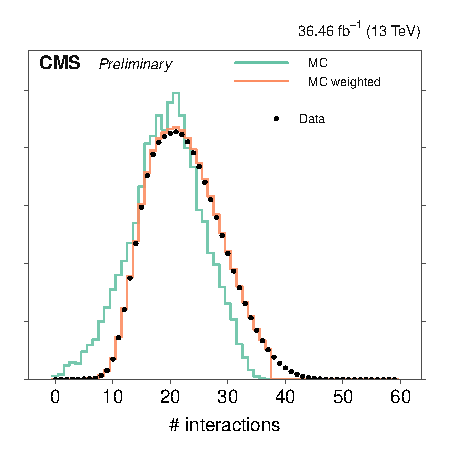
\includegraphics[scale=1.00]{figures/pileup_reweighting/f044_corr_nTrueInt_data_mc_norm}
  \caption{The distribution of the average numbers of the inelastic
    interactions per colliding bunch pair per lumi section in the data,
    corresponding distribution in the simulated events, and that of the
    reweighted simulated events.} \label{f044_corr_nTrueInt_data_mc_norm}
\end{figure}


Figure~\ref{f044_corr_nTrueInt_data_mc_norm} shows the distributions
of \verb!nTrueInt! in the data, simulated events and reweighted
simulated events. The figure demonstrates that the reweighted
simulated events have the distribution of \verb!nTrueInt! nearly
identical to that in the data. 
We note that the simulation does not contain events with 37 or more
overlapping pp interactions, while the data do, causing the MC
weighted distribution not to match perfectly the data. This small
issue will be recovered once the new MC samples with updated PU
profile will be available.



\subsection{Cross sections for SM samples}
\label{sec:SMxs}
This analysis chooses to use \MADGRAPH samples binned in partonic \HT 
for the set of MC samples (W+jets, DY+jets, QCD, $\gamma$+jets, $Z\rightarrow \nu\nu$+jets).
These binned samples are provided with LO cross sections. 
The \kfactors required to go from LO to NNLO cross section are typically determined using corresponding
inclusive samples applied to each \HT binned sample.
The inclusive distributions of the MC samples
with respect to the binning variable
$H_{T}^{parton}$ are shown in Fig.~\ref{fig:Lhe_Ht}, with
the bin by bin derivative drawn below. 
As can be seen in the distributions, the stitched samples
exhibit a good level of smoothness,
further demonstrated by the derivative which shows a flat trend for each 
cross section.

As described in Section~\ref{sec:mc-corrections}, residual cross
section corrections are measured using data in sidebands designed to
enrich specific SM processes. These corrections can prove to be
important for the closure test procedures described in Section
\ref{sec:closure-tests}.

\begin{figure}[!h]
  \begin{center}
    \subfigure[$Z\rightarrow \nu\nu$ +jets] {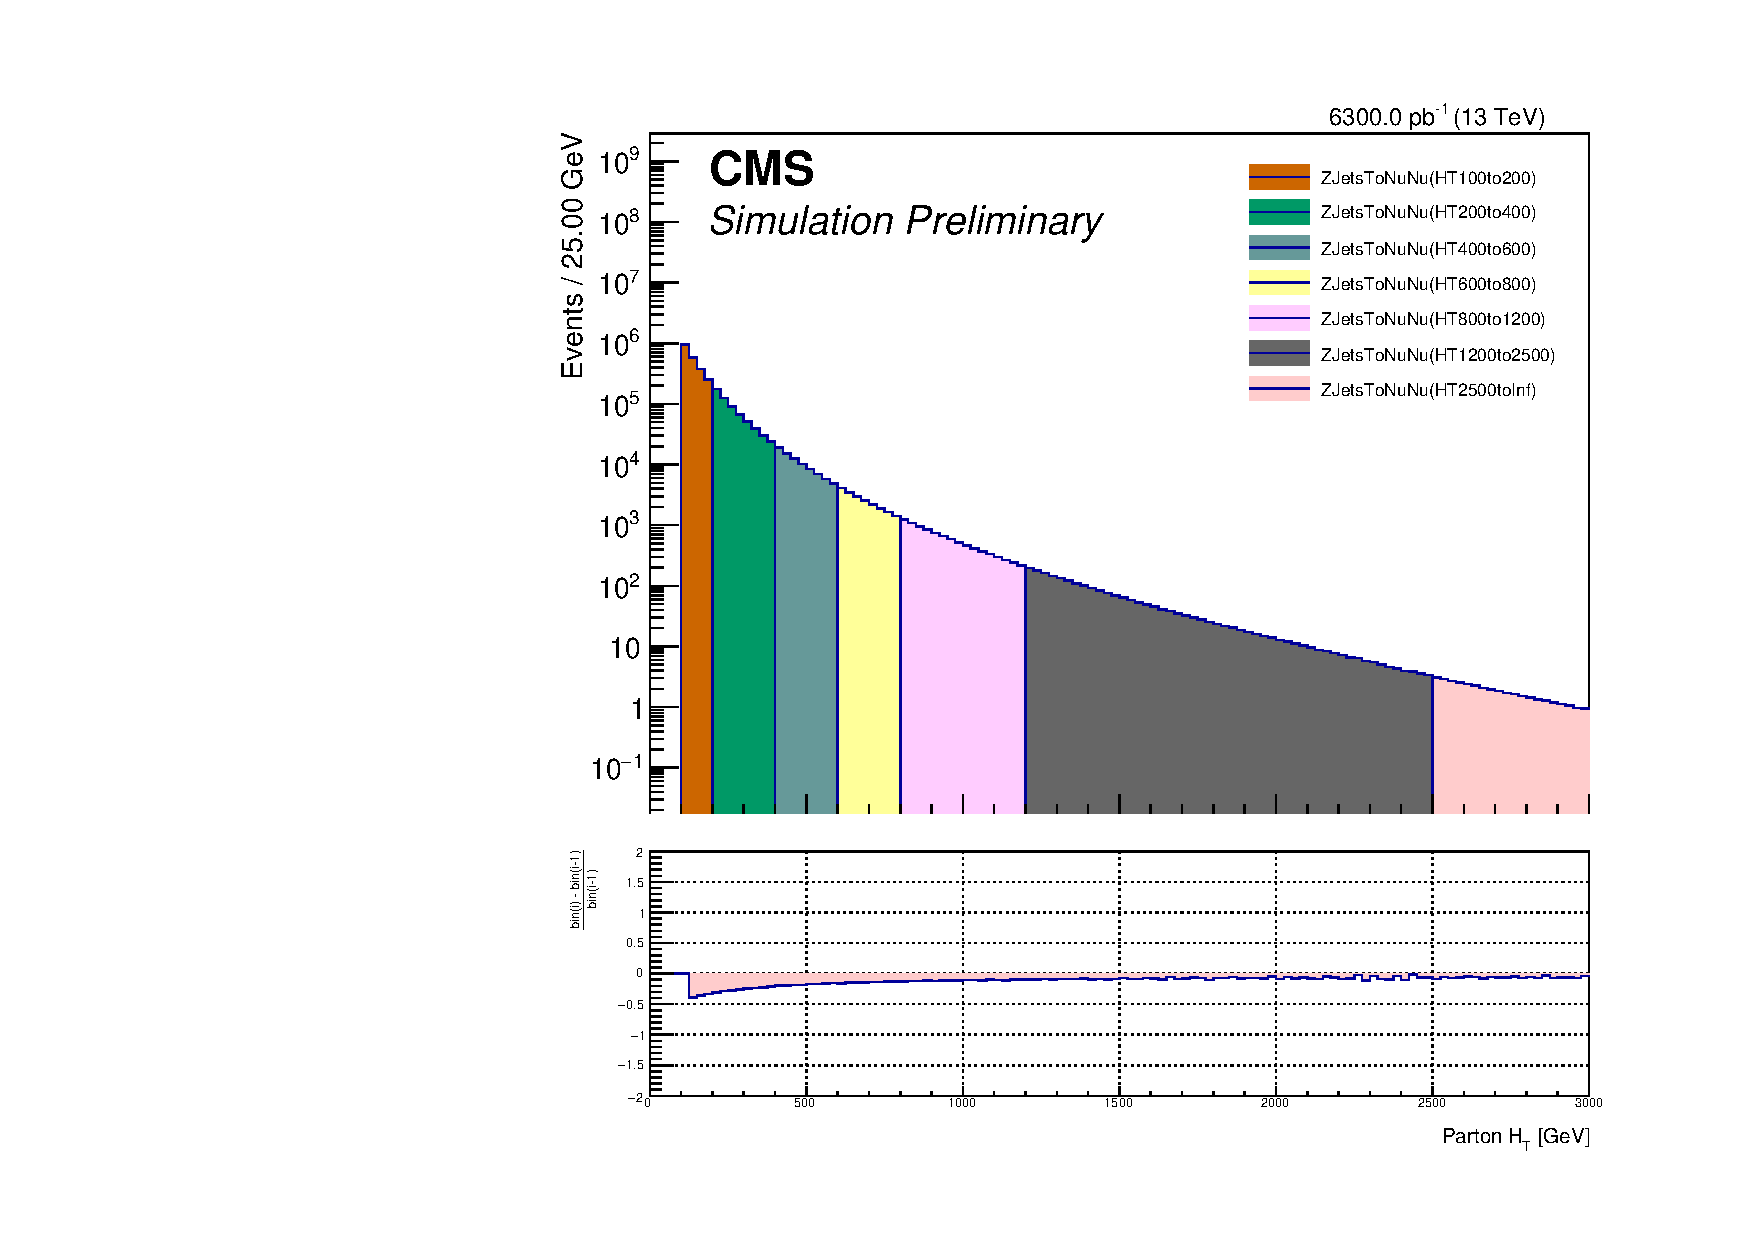
\includegraphics[width=0.40\textwidth]{figures/binnedMCsamples/2016/6p3/Zinv.pdf}} ~~
    \subfigure[$W\rightarrow l \nu$ + jets]{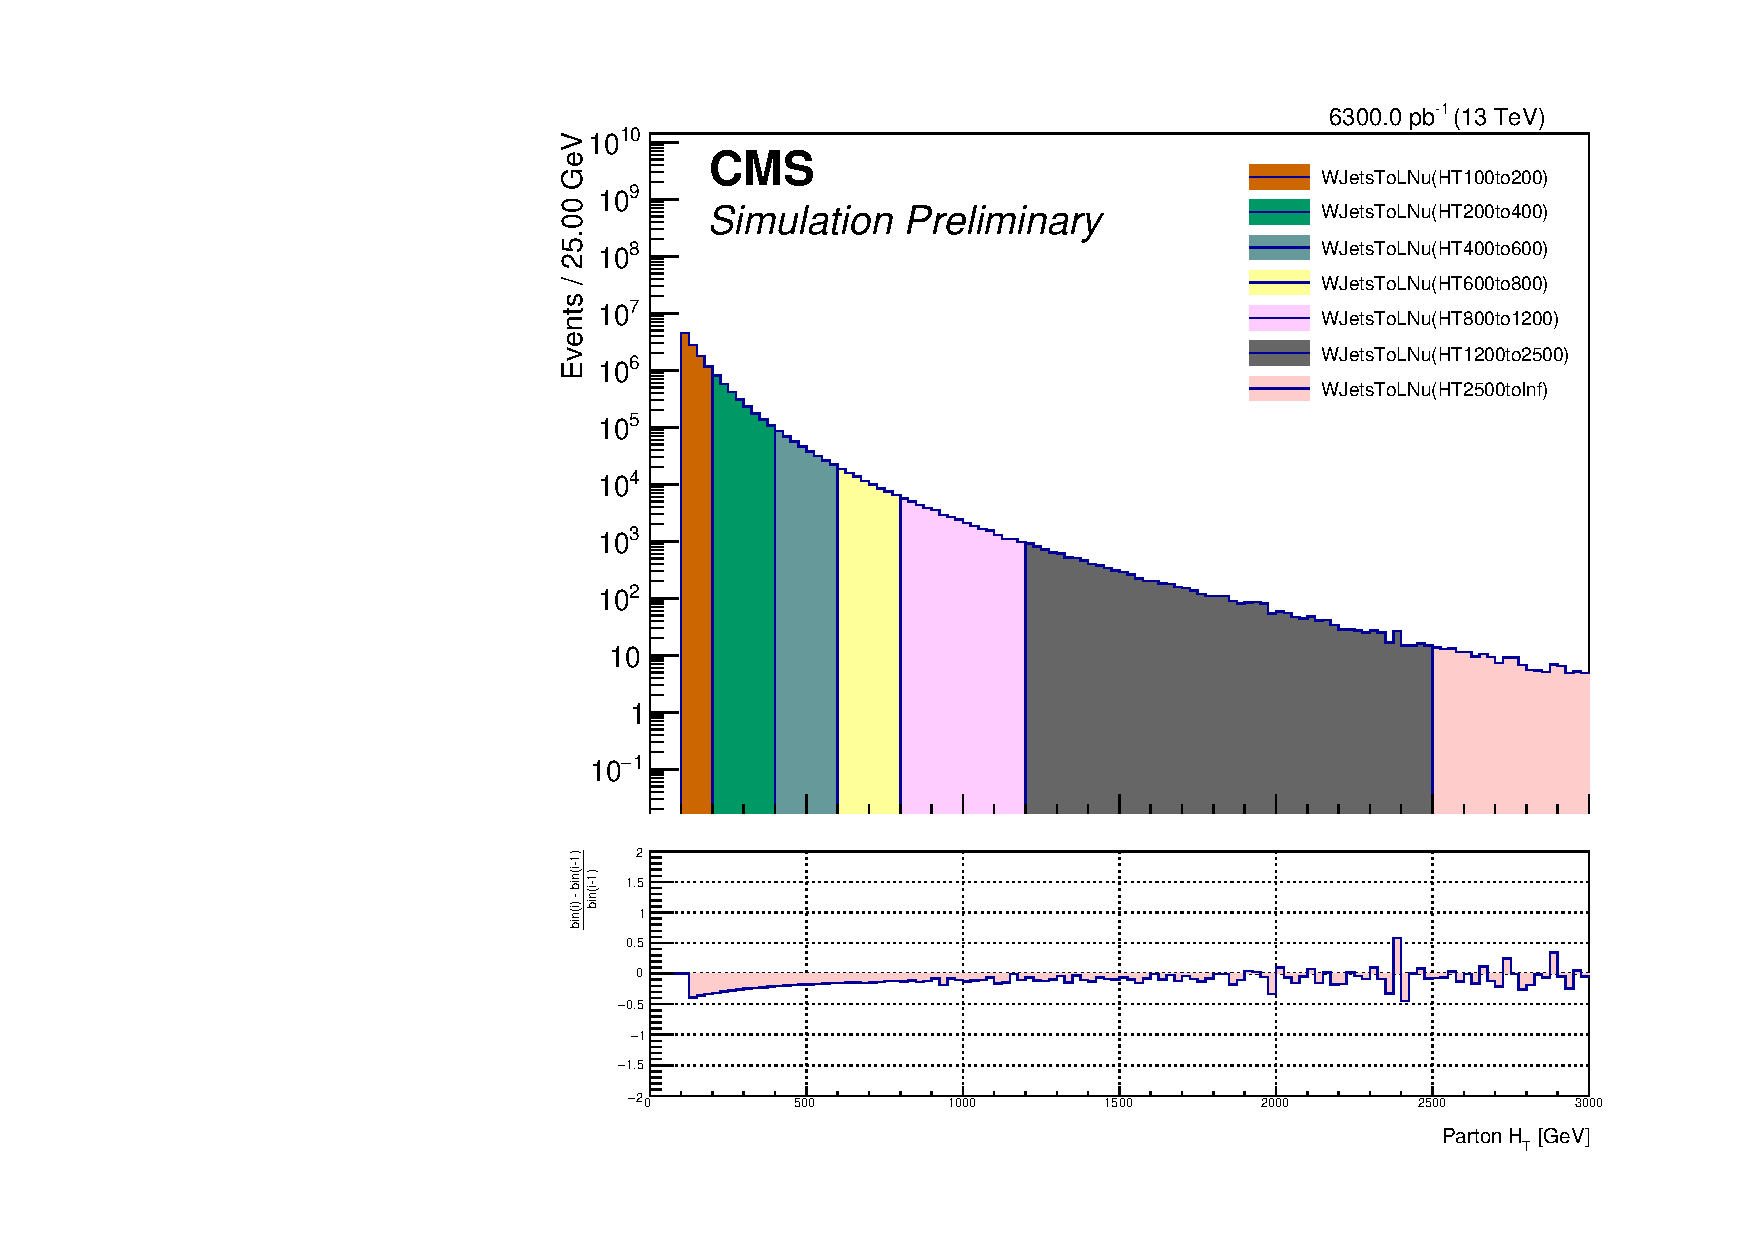
\includegraphics[width=0.40\textwidth]{figures/binnedMCsamples/2016/6p3/WJetsToLNu_HT.pdf}} \\
    \subfigure[$DY\rightarrow ll$ + jets]{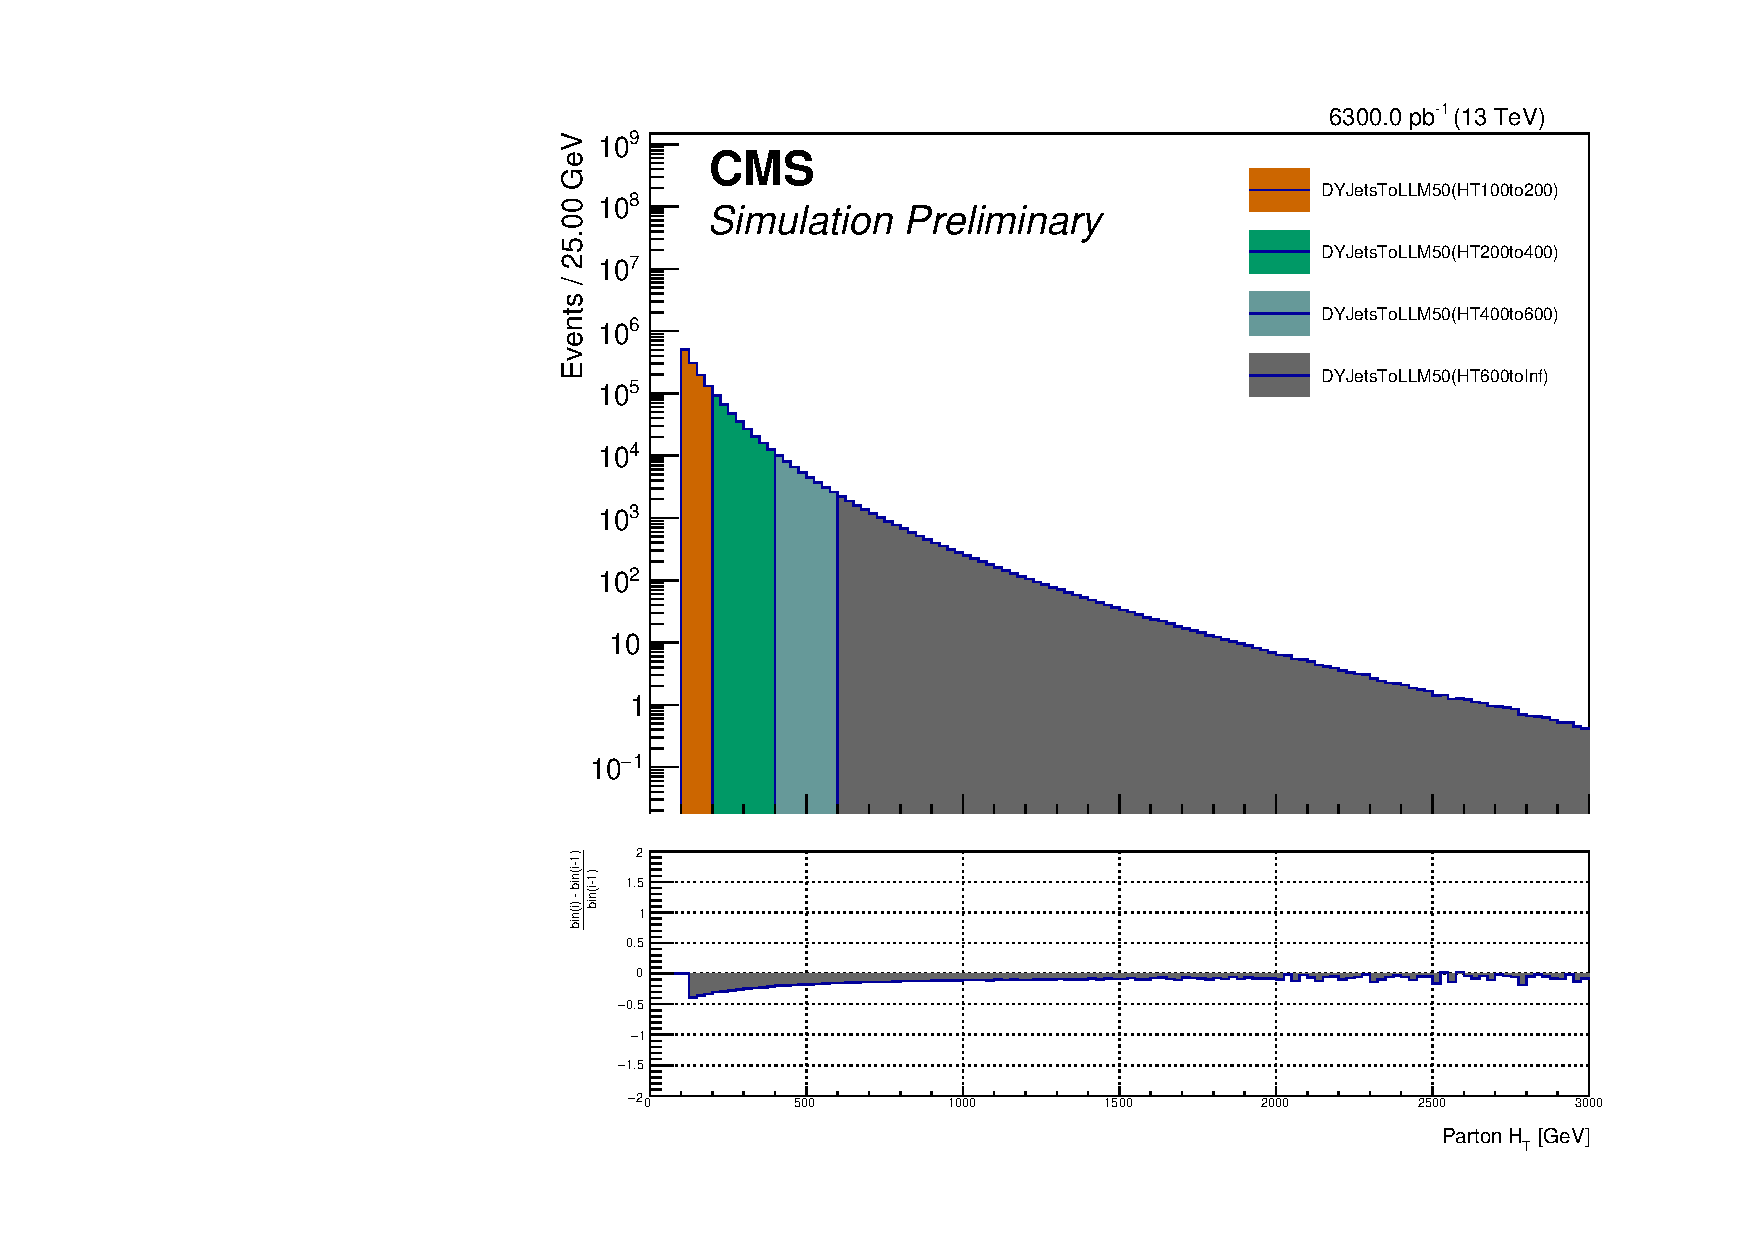
\includegraphics[width=0.40\textwidth]{figures/binnedMCsamples/2016/6p3/DYJetsToLL_M50_HT.pdf}} ~~
    \subfigure[QCD]{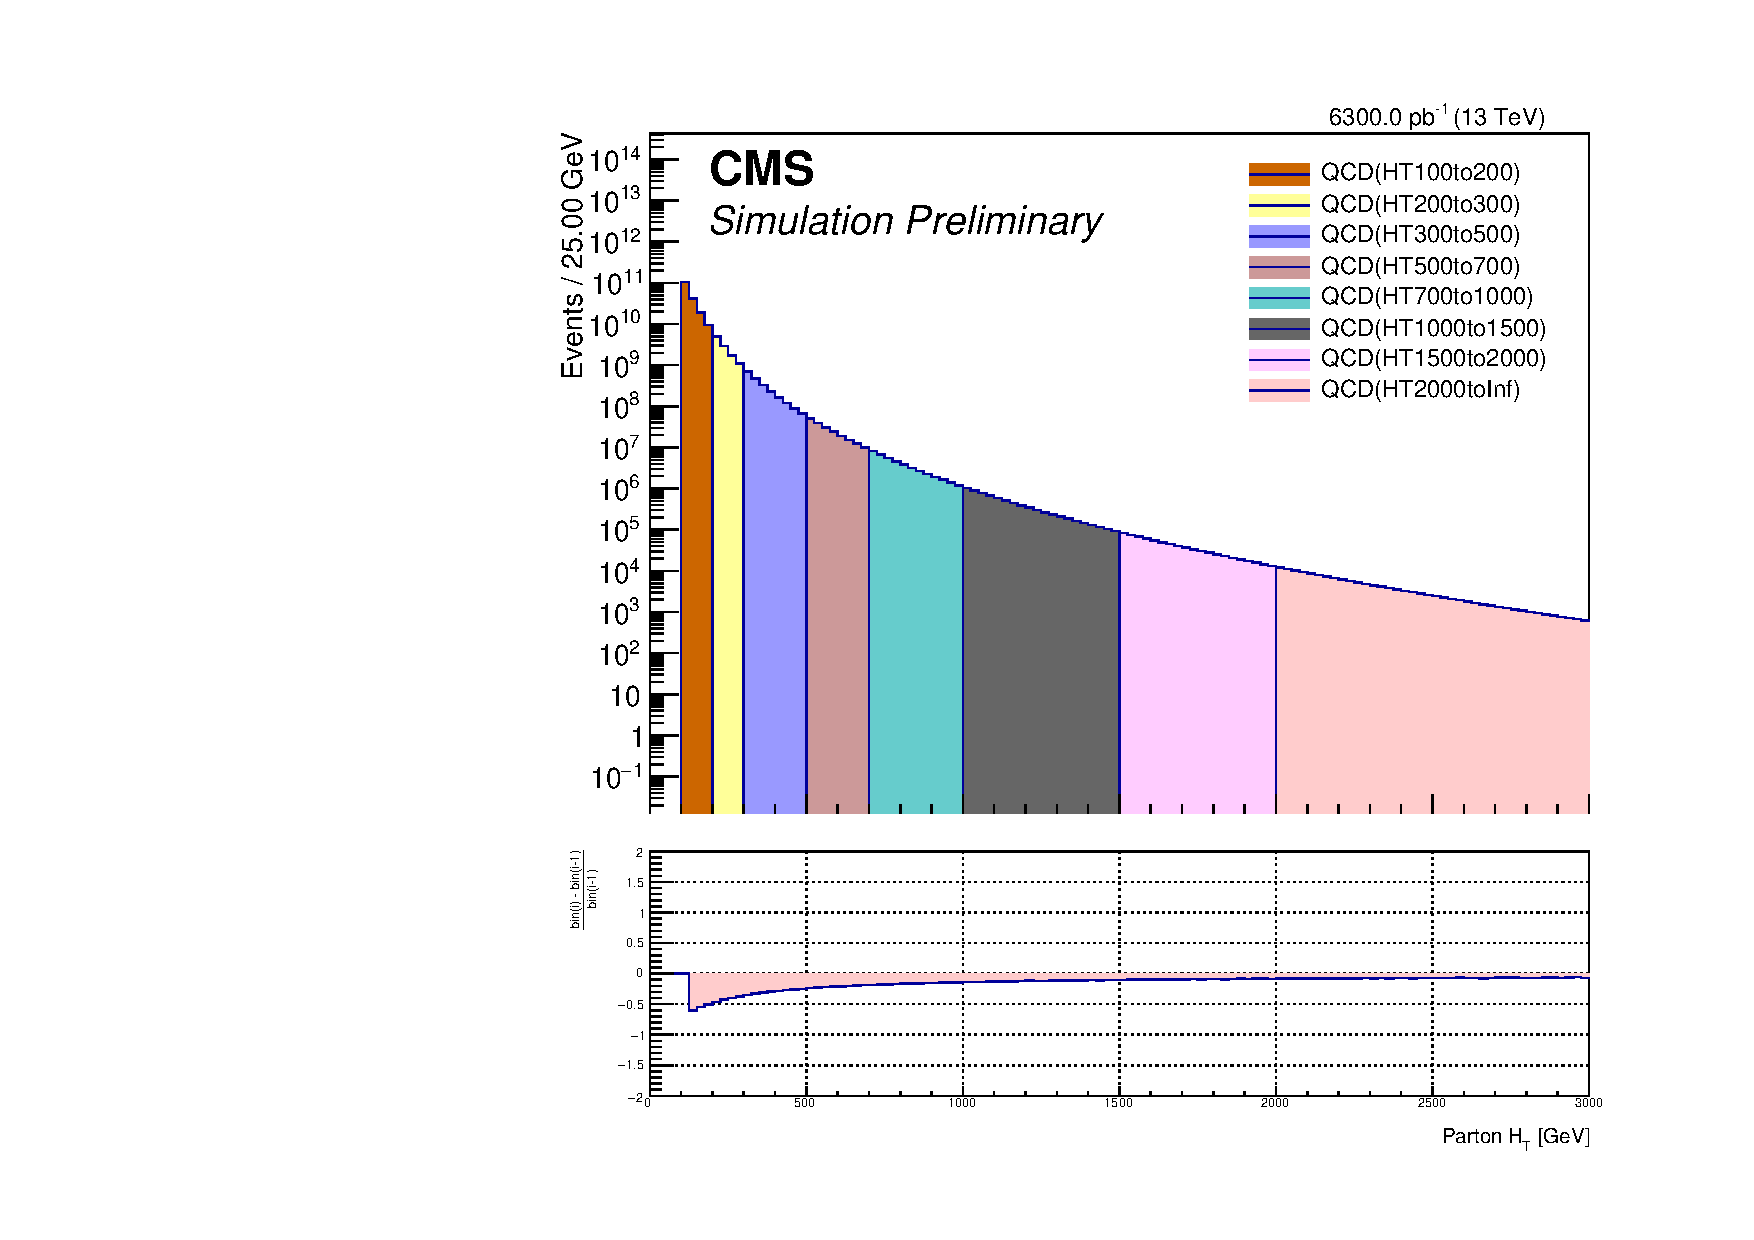
\includegraphics[width=0.40\textwidth]{figures/binnedMCsamples/2016/6p3/QCD_HT.pdf}} \\
    \subfigure[$\gamma$+jets]{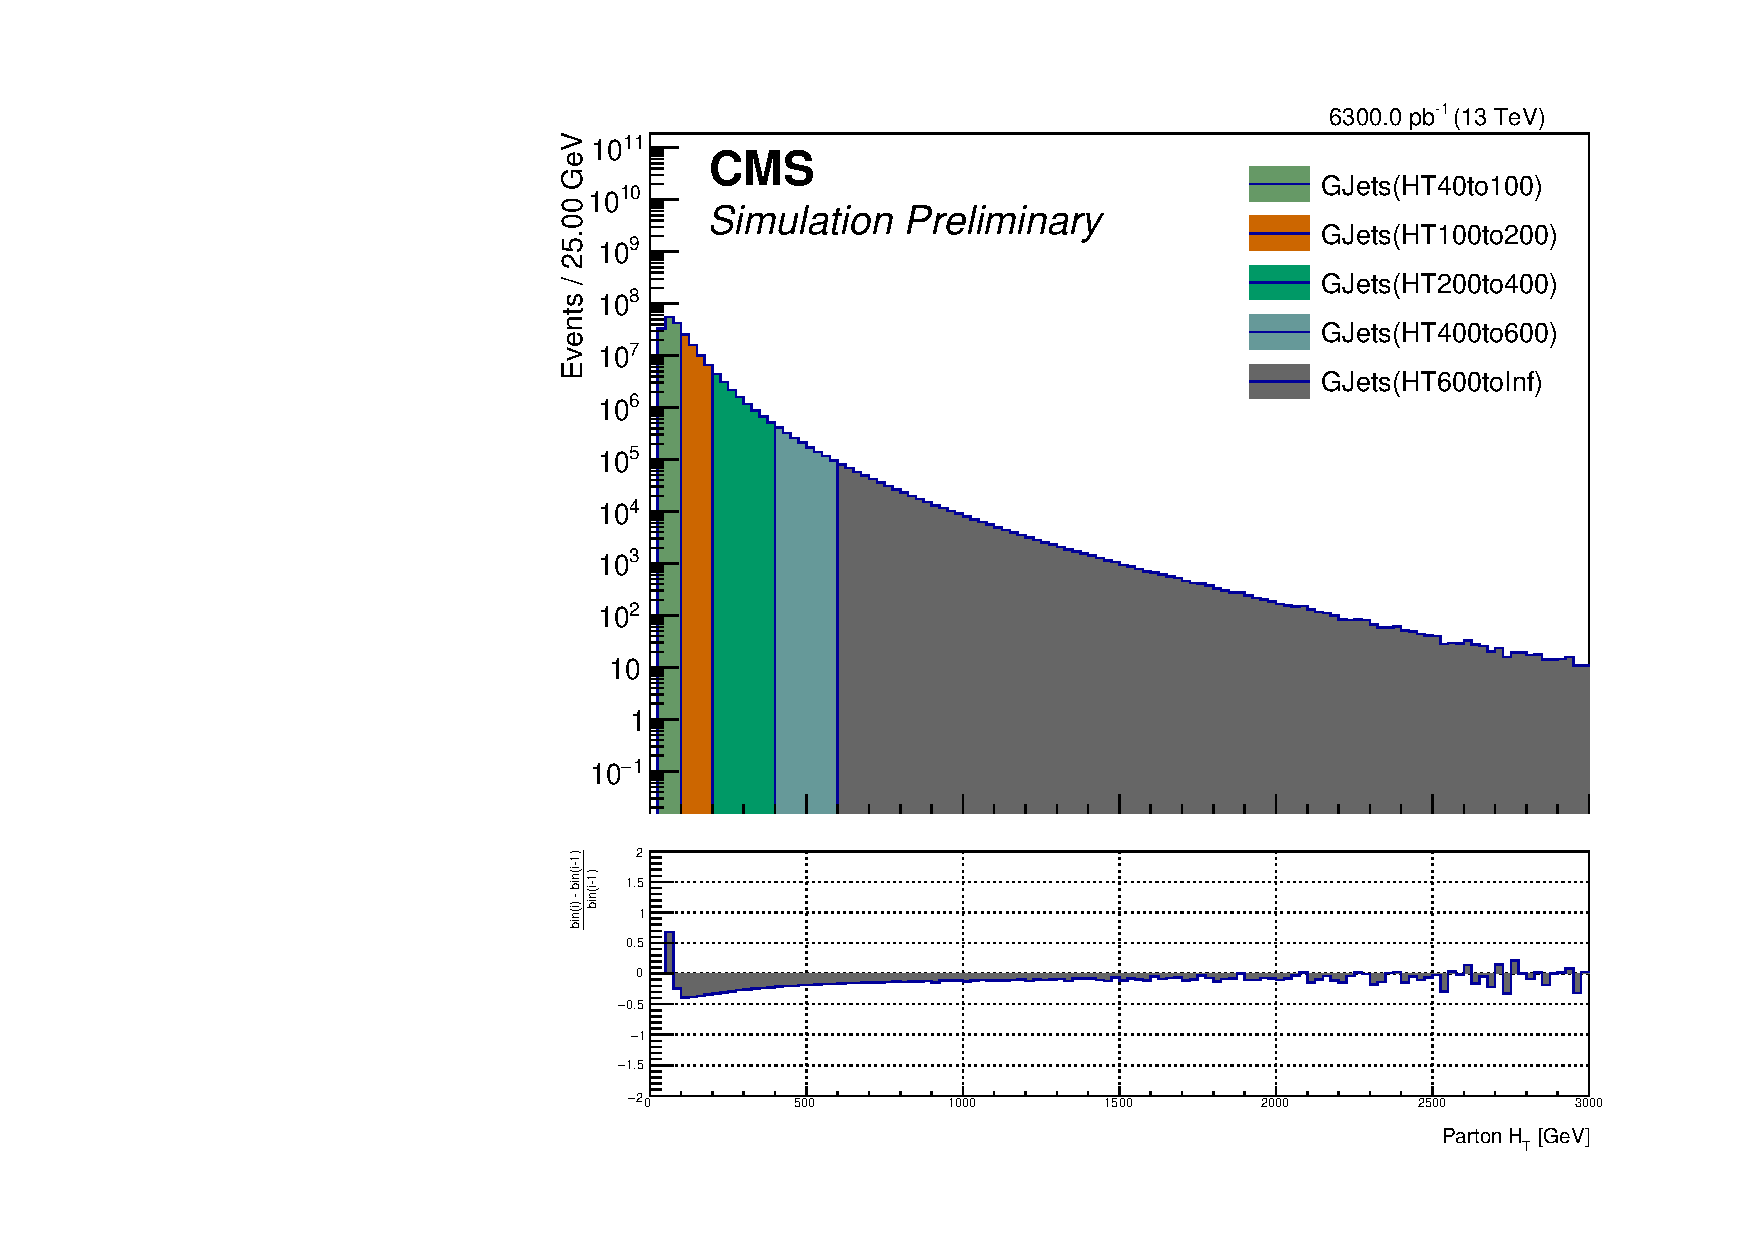
\includegraphics[width=0.40\textwidth]{figures/binnedMCsamples/2016/6p3/GJets_HT.pdf}} ~~
    \caption{Generator-level $H_{T}^{parton}$ distributions for SM process, $Z\rightarrow \nu\nu$ + jets, W+jets, DY+jets, QCD and $\gamma$+jets}
    \label{fig:Lhe_Ht}
  \end{center}
\end{figure}

%%____________________________________________________________________________||

%%____________________________________________________________________________||
\section{Trigger strategy}
\label{sec:triggers}

\subsection{Signal regions\label{sec:hadronic_signal_region}}

In Run~2, the RA1 analysis retains low thresholds comparable to those
used during Run~1 with developments to the trigger selection,
maintaining sensitivity to signatures of new physics with hadronic
energies as low as $\scalht = 200$ GeV. This in part is achieved by a
migration to PF-based jet reconstruction within the HLT which, in
conjunction with a reduction of clustering radius parameter $\Delta R
= 0.4$, provides improvements in jet energy resolution in high-pileup
conditions and mitigates the effects of pileup contamination within
the jet cone.

The RA1 analysis utilises a range of triggers for the selection of
events in the hadronic signal region to provide coverage over a wide
range of event topologies. A guiding principle of the analysis is to
be as inclusive as possible by maintaining low online and offline
thresholds. 

A suite of cross-triggers of the form
\verb!HLT_PFHTXXX_PFDijetAveYYY_AlphaT0pZZ!, comprising requirements
on \scalht, \alphat, and the average \pt of the leading two jets, are
used to record candidate signal events. The jets considered by these
cross-triggers satisfy $\Pt > 40\GeV$ and $|\eta| < 3.0$. A further
cross-trigger, \verb!HLT_PFMETNoMuXX_PFMHTNoMuXX_IDTight!  comprising
requirements on \MET, \HTmiss, and the presence of a jet with $|\eta|
< 3.0$, as well as a single-object \scalht trigger, are also employed
to record candidate signal events. The trigger requirements and
thresholds are summarised in
Table~\ref{tab:2015_Hadronic_Signal_Triggers}.

%The use of a \pt-averaged threshold of the two leading jets suppresses
%the QCD multijet background while providing acceptance to events
%exhibiting asymmetric jet topologies, such as monojet-like signatures
%of compressed spectrum and DM models. It was found that a dijet
%average threshold of 90 \GeV ensured the optimum performance when
%balancing efficiency and rate, with both the $\scalht$ and $\alphat$
%thresholds across all jet topologies. The dijet average requirement
%does however lead to a loss in efficiency for asymmetric jet events
%where the sub-leading jet is soft.
%This loss in efficiency is mitigated by taking the disjunction of the
%\alt and monojet triggers which provides a recovery of efficiency in
%the turn-on and close to the plateau for the low-\scalht asymmetric
%categories.  

%The Level-1 seeds for the $\scalht$--$\alphat$ HLT paths are given by
%the disjunction of all available hadronic scalar energy and missing
%energy sum seeds for the given run scenario. A loose calorimeter
%trigger prefilter is utilised to reduce the pass-through rate prior to
%track-based reconstruction, ensuring the PF-based filters meet timing
%requirements. The calorimeter prefilter utilises loose \scalht and
%dijet average \pt requirements in addition to a new variable \alphat',
%defined as \alphat in the limit $\Delta\scalht \rightarrow 0$, which
%better correlates \alphat between calorimeter and PF-based
%reconstruction.

%The choice of threshold for the \scalht--\alphat triggers were tuned
%to maintain acceptance for a range of signal topologies whilst
%effectively suppressing QCD multijet events to maintain acceptable
%trigger rates.

\begin{table}[h!]
  \topcaption{Summary of the L1 seeds and HLT trigger paths used by
    the analysis. The lowest and highest (in parentheses) thresholds
    used for each HLT trigger path during the 2016 data taking period
    are given. } 
  \footnotesize
  \centering
\begin{tabular}{l|l} 
  \hline
  \hline
  L1 seed & HLT path \\
  \hline
  {\scriptsize\verb!HTT or ETM!} & {\scriptsize\verb!HLT_PFHT200_PFDijetAve90_AlphaT0p57(65)!} \\
  {\scriptsize\verb!HTT or ETM!} & {\scriptsize\verb!HLT_PFHT250_PFDijetAve90_AlphaT0p55(57)!} \\
  {\scriptsize\verb!HTT or ETM!} & {\scriptsize\verb!HLT_PFHT300_PFDijetAve90_AlphaT0p53(55)!} \\
  {\scriptsize\verb!HTT or ETM!} & {\scriptsize\verb!HLT_PFHT350_PFDijetAve90_AlphaT0p52(53)!} \\
  {\scriptsize\verb!HTT or ETM!} & {\scriptsize\verb!HLT_PFHT400_PFDijetAve90_AlphaT0p51(52)!} \\
  {\scriptsize\verb!HTT!}        & {\scriptsize\verb!HLT_PFHT800(900)!} \\
  {\scriptsize\verb!ETM!}        & {\scriptsize\verb!HLT_PFMETNoMu90(110)_PFMHTNoMu90(110)_IDTight!} \\
  \hline
  \hline
\end{tabular}
\label{tab:2015_Hadronic_Signal_Triggers}
\end{table}

%An important goal of the analysis is to have good acceptance to
%compressed SUSY and general DM models. It is therefore critical that
%we operate in the trigger turn on regions for the lower thresholds. We
%have already successfully exercised this approach with the Run 1
%analysis and will repeat this mode or operating during Run 2.  As in
%Run~1, multiple efficiency measurements are employed, which are
%performed with data and propagated through to the analysis with cross
%checks in simulation.

The efficiency of the signal triggers are measured in data using event
samples containing an electron and muon, recorded with unprescaled
electron and muon ``reference'' triggers and defined by a
signal-region-like selection criteria (when ignoring the lepton in the
computation of event-level variables, such as \scalht or \MET). Biases
in these measurements can be introduced due to the contamination in
the computation of event-level variables and different treatments
between trigger and offline reconstructions, the degree of which
varies with \scalht and \njet. In the case of efficiency measurements
using the electron reference trigger, no cross-cleaning of electrons
from jets is performed offline, with the electron being included in
the computation of event-level jet energy sums, such as \scalht, \MHT
and \alt. When using the muon reference triggers, offline
cross-cleaning of the muons is performed. 

The trigger efficiency as a function of \mht for the full suite of
triggers, as determined from the data samples described above, is
shown per \scalht bin (following the \scalht binning scheme of the
signal region) in Fig.~\ref{fig:alphat_turnons} (in
Appendix~\ref{sec:triggers}). The figure contains efficiency curves
determined from both the muon and electron event samples. Significant
differences are visible in the turn-on region, due to the
cross-cleaning issues through the various steps of the
trigger--analysis chain (L1, HLT Calo-based pre-filter, HLT PF-based
decision, offline) as described above. However, the efficiencies are
close to 100\% for the requirement $\HTmiss > 200\GeV$, as illustrated
by Table~\ref{tab:trigger-eff}, which is now the default \HTmiss
requirement used in this analysis. The measured efficiencies and their
uncertainties are applied as corrections to the MC samples. The
central value of the correction is taken from the efficiency measured
with the electron reference trigger. The statistical uncertainties in
the central values, as well as the difference in efficiencies between
those measured with the electron and muon triggers, are propagated.

\begin{table}[h!]
  \topcaption{Efficiency of the full suite of signal triggers as a
    function of \scalht after applying the signal region selection
    criteria, determined from $e$ + jets and \mj event samples.
  } 
  \footnotesize
  \centering
  \begin{tabular}{lccccc} 
    \hline
    \hline
    Event sample & \multicolumn{5}{c}{\scalht bin [GeV]}                                              \\
    \cline{2-6}
                 & 200--400       & 400--600       & 600--900       & 900--1200      & $>$1200        \\
    \hline
    $e$ + jets   & $99.0 \pm 0.5$ & $99.0 \pm 0.5$ & $99.0 \pm 0.5$ & $99.0 \pm 0.5$ & $99.0 \pm 0.5$ \\
    \mj          & $99.0 \pm 0.5$ & $99.0 \pm 0.5$ & $99.0 \pm 0.5$ & $99.0 \pm 0.5$ & $99.0 \pm 0.5$ \\
    \hline
    \hline
  \end{tabular}
  \label{tab:trigger-eff}
\end{table}

\subsection{Control regions\label{sec:control_samples}}

The \mj and \mmj control samples are selected with the logical OR of
the \verb!HLT_IsoMu22!, \verb!HLT_IsoTkMu22!, \verb!HLT_IsoMu24! and
\verb!HLT_IsoTkMu24! triggers. The trigger efficiencies are provided
by the muon POG and are determined by the muon for both data and
simulated samples (containing a trigger emulation) using a tag and
probe method. The POG also provide data-to-simulation scale factors,
which we apply to the trigger-efficiency-corrected event yields from
simulation. The \Pt- and $\eta$-averaged triggers efficiencies
determined per (\njet, \nb, \scalht) bin for the \mj sample are
typically and rather independent of \njet, \nb, and \scalht. For the
\mmj sample, the average efficiencies are $\sim99\%$ (as either muon
can provided the positive trigger decision). Statistical and
systematic uncertainties are propagated through via the scale factor
corrections, following the prescription from the muon POG.

The \gj event sample is recorded with an \verb!OR! of the
\verb!HLT_Photon175! and \verb!HLT_ECALHT800! triggers. The efficiency
is measured as a function of both photon \Pt and \HTmiss for events in
the JetHT data set satisfying the \gj control region selection, as
shown in Fig.~\ref{fig:photon_turnons_photonPt}. The single photon
trigger alone exhibits a decreasing efficiency with increasing photon
\Pt, which is attributed to an H/E cut at Level 1. The inefficiency
can be largely recovered by also employing the \verb!ECALHT800!
trigger. In this way, the inefficiency can be recovered for photon
$\Pt > 600\GeV$. The photon efficiency is $\sim 98\%$. The
efficiencies are used to correct the simulated event counts in the \gj
sample, and a systematic uncertainty is assumed to be the magnitude of
the inefficiency ($\sim 2\%$).

\fixme{WHAT ABOUT THE QCD SIDEBAND TRIGGER EFFS??}

%%____________________________________________________________________________||

%%____________________________________________________________________________||
\section{Physics objects}
\label{sec:objects}
The definitions of the physics objects used in this analysis follow the recommendations of the various Physics Object Groups (POGs). 
During data taking these recommendations are subject to change and will be be updated if necessary.

\subsection{Jets}
\label{sec:jetreco}
Jets are defined as sets of particle-flow (PF) candidates clustered by the
anti-$k_{T}$ jet clustering algorithm \cite{Cacciari:2008gp} with a distance parameter of 0.4
(PFJets). Charged Hadron Subtraction (CHS) is applied, i.e., charged
hadrons that can be traced back to pileup vertices are not clustered.
The four-momenta of jets are initially defined as the four-vector sum of
the four-momenta of the constituent particle-flow candidates and then
scaled by the jet energy correction factors designated as L1FastJet,
L2Relative, and L3Absolute \cite{Chatrchyan:2011ds}.

The ``loose'' working point Jet-Id selection criteria is chosen. 
The cuts are listed in Tab.~\ref{tab:loose-jet-id}. 
In addition, a dedicated selection is applied to reject ``beam halo'' candidate events, 
as described in Section~\ref{sec:had-signal}.

\begin{table}[ht!]
  \caption{The ``loose'' jet ID requirements. \label{tab:loose-jet-id}}
  \centering
  \begin{tabular}{ ccc }
    \hline
    \hline
    Variable & cut & notes \\ \hline
    \multicolumn{3}{c}{$-3.0 < \eta_{\mathrm{jet}} < 3.0$} \\ \hline    
    Neutral Hadron Fraction & $<0.99$ & - \\
    Neutral EM Fraction & $<0.99$ & - \\
    Number of constituents & $>1$ & - \\
    Charged Hadron Fraction & $>0$ & only for $|\eta_{\mathrm{jet}}| < 2.4$ \\
    Charged Multiplicity & $>0$ & only for $|\eta_{\mathrm{jet}}| < 2.4$ \\
    Charged EM Fraction & $<0.99$ & only for $|\eta_{\mathrm{jet}}| < 2.4$ \\ \hline
    \multicolumn{3}{c}{$|\eta_{\mathrm{jet}}| > 3.0$} \\ \hline        
    Neutral EM Fraction & $<0.90$ & - \\
    Number of Neutral Particles & $>10$ & - \\
    \hline
    \hline
  \end{tabular}
\end{table}

\subsection{b-tagged jets}
\label{sec:btags}
Jets originating from bottom quarks are identified through vertices
that are displaced with respect to the primary interaction
\cite{Chatrchyan:2012jua}.  The algorithm used to tag b-jets is the
Combined Secondary Vertex tagger V2, with the ``medium'' working
point, which is achieved by requiring a cut of $>$ 0.800 on the
algorithm discriminator variable.  This results in a gluon/light-quark
mis-tag rate of $\sim$1 \% (where ``light'' means $u$, $d$ and $s$
quarks), a charm-quark mis-tag rate of $\sim$10 \% and a b-quark b-tag
efficiency of about 60 \%. 

Some validation studies used by the analysis make use of the ``loose''
and ``tight'' working points, which are defined by the thresholds
requirements of 0.460 and 0.935 on the discriminator variable. These
requirements yield light-flavour mistag probabilities of $\sim$10 and
$\sim$0.1\%, respectively.


\subsection{Muons}
\label{sec:muon-id}
Muons are selected in the \mj and \mmj control regions using the ``tight'' working point 
definition of the recommended identification algorithm from the Muon POG. 
Muons are also required to be well isolated, i.e. with a low activity in the vicinity of their track. 
The transverse momenta of PF neutral and charged candidates, as well as photons, lying within a cone around the lepton are summed. 
The relative combined isolation $I^{rel}_{comb}$ is then defined as 
the ratio of this scalar sum to the transverse momentum of the lepton
candidate. Additionally, $\rho\times A_{eff}$ corrections are applied to
remove the effects of pileup.
Muons are defined to be isolated if they fulfill the criterium $I^{rel}_{comb} < 0.15$. 

For the purpose of vetoing muons in the signal region, the ``loose'' working point 
is used, which provides $\sim$ 98 $\%$ efficiency. 
In the hadronic signal region a variable cone size for the isolation is used, which is referred to as ``mini-isolation''. 
This isolation algorithm helps in recovering some efficiency in the lepton selection for boosted topology of top quark decays, 
in which the muon's track may be found close to the jet activity due to the boost of the parent top. 
Therefore, the cone size used for the calculation of the lepton isolation is reduced as a function of 
the lepton \Pt, as follows: $R=0.2$ for $\Pt_{\ell}\leq50\gev$,
$R=10\gev/\Pt_{\ell}$ for $50 \gev < \Pt_{\ell} < 200\gev$ and $R=0.05$ for $\Pt_{\ell} > 200 \gev$.
In the signal region, identified muons with mini-isolation satisfying $I^{rel}_{comb} < 0.2$ are vetoed.


\subsection{Photons}
\label{sec:photon-id}
Photons are identified according to the ``tight'' working point definition ($\sim$ 71 $\%$ efficiency) 
of the simple cut-based photon identification algorithm \cite{photon-id} 
and required to be well isolated. 
A PF-based isolation is used with a cone size $\Delta R$ $<$ 0.3 and
$\rho\times A_{eff}$ corrections are applied to remove the effects of pileup \cite{pf-photon}. 
Table \ref{tab:photon-id-gamma} summarises the identification and isolation selection used. 

Photons are vetoed in the definition of the hadronic signal region and
muon control regions, as described in Sec.~\ref{sec:preSelection},
while a control region with one photon (``\gj'') is defined for the
purpose of the background estimation, as described in
Sec.~\ref{sec:photoncontrolSelection}.


\begin{table}[ht!]
  \caption{Photon identification selection.\label{tab:photon-id-gamma}}
  \centering
  \footnotesize
  \begin{tabular}{ ccc }
    \hline
    \hline
    Categories & \multicolumn{2}{c}{Barrel}   \\
    Working point  & Tight & Loose \\
    \hline
    Conversion safe electron veto & Yes & Yes  \\
    Single Tower H/E              & 0.05 & 0.05  \\
    $\sigma_{i\eta i\eta}$        & 0.0100 & 0.0102 \\
    PF charged hadron isolation   & 0.76 & 3.32  \\
    PF neutral hadron isolation   & 0.97 + 0.014 $\times$ $p_{\mathrm{T},\gamma}$ + 0.000019 $\times$ $p_{\mathrm{T},\gamma}^{2}$ & 1.92 + 0.014 $\times$ $p_{\mathrm{T},\gamma}$ + 0.000019 $\times$ $p_{\mathrm{T},\gamma}^{2}$  \\
    PF photon isolation           & 0.08 + 0.0053 $\times$ $p_{\mathrm{T},\gamma}$ & 0.81 + 0.0053 $\times$ $p_{\mathrm{T},\gamma}$ \\
    \hline
    \hline
    Categories & \multicolumn{2}{c}{Endcap}   \\
    Working point  & Tight & Loose \\
    \hline
    Conversion safe electron veto & Yes & Yes  \\
    Single Tower H/E              & 0.05 & 0.05  \\
    $\sigma_{i\eta i\eta}$        & 0.0268 & 0.0274 \\
    PF charged hadron isolation   & 0.56 & 1.97  \\
    PF neutral hadron isolation   & 2.09 + 0.014 $\times$ $p_{\mathrm{T},\gamma}$ + 0.000025 $\times$ $p_{\mathrm{T},\gamma}^{2}$ & 11.86 + 0.014 $\times$ $p_{\mathrm{T},\gamma}$ + 0.000025 $\times$ $p_{\mathrm{T},\gamma}^{2}$ \\
    PF photon isolation           &  0.16 + 0.0034 $\times$ $p_{\mathrm{T},\gamma}$ & 0.83 + 0.0034 $\times$ $p_{\mathrm{T},\gamma}$ \\
    \hline
    \hline
  \end{tabular}
  \end{table}


\subsection{Electrons}
\label{sec:electron-id}
In order to veto electrons in the hadronic signal region and the muon
and photon control regions, the ``loose'' working point definition
($\sim$ 90 $\%$ efficiency) of the cut-based electron identification
\cite{electron-id} is used.  Electrons are also require required to be
isolated.  Similar to muons, in the hadronic signal regions a PF-based
isolation \cite{pf-photon} is used with a cone size determined by the
mini isolation algorithm (see Sec.~\ref{sec:muon-id}) and $\rho\times
A_{eff}$ corrections are applied to remove the effects of pileup.
Isolated electrons are defined by $I^{rel}_{comb} < 0.1$.

Table \ref{tab:ele-id} summarises the identification 
selection used. 

\begin{table}[h!]
  \caption{Electron identification (``tight'' working point).\label{tab:ele-id}}
  \centering
  \footnotesize
  \begin{tabular}{ lcc }
    \hline
    \hline
    Categories                                               & Barrel    & EndCap    \\
    \hline
    $\Delta \eta_{In}$                                       & 0.0105   & 0.00814  \\
    $\Delta \phi_{In}$                                       & 0.115    & 0.182  \\
    $\sigma_{i\eta i\eta}$                                   & 0.0103    & 0.0301  \\
    H/E                                                      & 0.104    & 0.0897   \\
    d0 (vtx)                                                 & 0.0261    & 0.118  \\
    dZ (vtx)                                                 & 0.041    & 0.822  \\
    $\lvert(1/E_{\textrm{ECAL}} - 1/p_{\textrm{trk}})\rvert$ & 0.102     & 0.126  \\
    Missing hits (inner tracker)                             & 2         & 1         \\
    Conversion veto                                          & yes       & yes   \\
    \hline
    \hline
  \end{tabular}
  \end{table}


\subsection{Single isolated tracks}
\label{sec:SIT}
A single isolated track (SIT) can be used to identify W bosons through their leptonic decays: 
W $\rightarrow$ $\mu \nu$, W $\rightarrow$ $e\nu$, and W $\rightarrow$ $\tau$($\rightarrow l$) $\nu$. 
Single prong decays of the tau lepton can also be identified: W $\rightarrow$ $\tau$ ($\rightarrow$ h$^{\pm}$ + n$\pi^{0}$) $\nu$. 
A single isolated track comprises a charged PF candidate with $\Pt > 10 \gev$, $\Delta z(\mathrm{track}, \mathrm{PV}) < 0.05 \, \mathrm{cm}$ 
and with a relative isolation smaller than 0.1, where the isolation is determined from the sum 
of the \Pt of the charged PF candidates within $\Delta R < 0.3$.
%Events in the signal region and all control regions (ignoring the
%selected muons) containing a SIT candidate identified with these
%criteria are vetoed.


\subsection{Missing transverse momentum}
Missing transverse momentum (\met) is defined as the magnitude of the vector sum
of the transverse momentum of all particle-flow candidates in the event.
The Type-I \met correction \cite{Khachatryan:2014gga} is applied, i.e., the transverse momentum of
the particle-flow candidates clustered as jets are replaced with the
transverse momentum of the jets that are scaled by the jet energy
correction factors.

The \met is used in the definition of 
the transverse mass, $M_{T}$, which is in turn used as part of
the selection criteria that define the single muon control sample 
(Sec.~\ref{sec:mucontrolSelection}), and for the $\mhtmet$ cleaning filter, 
as described in Sec.~\ref{sec:selection}.



%%____________________________________________________________________________||

%____________________________________________________________________________||
\section{Event selection and categorisation for signal and control regions}
\label{sec:selection}

This section first outlines the set of ``pre-selection'' requirements
that are common to all signal and control regions, before defining the
selection criteria that are specific to each region.

%%____________________________________________________________________________||
\subsection{Pre-selection}
\label{sec:preSelection}

\subsubsection{MET filters}

A number of beam- and detector-related effects can induce significant
\met. Examples include beam halo, reconstruction failures, spurious
detector noise, or event misreconstruction due to detector
inefficiencies. These events, with large, non-physical values of \met,
are rejected with high efficiency by applying a range of dedicated
vetoes. All ``MET filters'' recommended by the JetMET POG and SUSY PAG
are applied by default in this analysis and listed in Table~\ref{tab:pre-selections}.

\subsubsection{Jet requirements}

Jets considered in the analysis are required to satisfy $\PT>40\gev$
and $|\eta|<2.4$. Events containing jets in the forward region that
satisfy the requirements $\PT>40\gev$ and $|\eta|>2.4$ are rejected (regardless of the identification requirement) 
in order to control background contributions from SM processes, without
introducing a significant reduction in signal acceptance. The selected jets 
are used in the calculation of all jet-based
event-level variables, such as \HT, \mht, and \alphat.

The lead jet is required to satisfy $\PT > 100\gev$. 
This helps to ensure high trigger efficiencies,
but also helps to improve the S/B for a wide
range of models with respect to SM processes, such as V + jets
production. Events are then classified based on the
second leading jet. In the case that a second leading jet satisfies $\PT > 100\gev$ 
events are assigned to a ``symmetric'' \njet category. If the second
jet satisfies $40 < \PT < 100\gev$ events are assigned to an
``asymmetric'' \njet category. Finally, if there is no other jet 
with $\PT>40\gev$, events are assigned to the ``mono-jet''
category. This categorisation is heavily utilised throughout all the document. \\
The asymmetric and mono-jet categories have been added to
the analysis to help improve acceptance to a range of DM models and compressed
SUSY.

\subsubsection{Jet-based energy sums}

Events are required to have significant hadronic activity by requiring
$\scalht > 200\GeV$. Despite an increase in both multijet production
cross sections and pileup in Run~2, the lowest \HT threshold is
kept at the same value of the Run~1 analysis~\cite{Chatrchyan:2013lya}
in order to maintain acceptance to DM models or compressed
SUSY. 

An estimator of the missing transverse energy for each event, \ETmiss,
is determined from the vectorial sum of the jet transverse momenta,
known as \mht. Events are required to have appreciable missing
transverse energy by requiring $\mht>130\gev$. This requirement is
applied to events in the signal and control regions. The
\scalht-dependent \alphat thresholds, required to suppress multijet
events as outlined in Sec.~\ref{sec:had-signal}, provide an effective
threshold on \mht comparable to 130\GeV via the relationship in
Eq.~(\ref{eq:alphat3}). Hence, the extrapolation from control to
signal region in \mht is minimal. 

\subsubsection{The \mht/\met variable}

Finally, the value of \mht is compared to the missing transverse
energy variable, $\met$. Only events that satisfy
$R_{\mathrm{miss}}=\mht/\met < 1.25$ are considered in order to
protect against events containing multiple jets outside the
experimental acceptance that contribute significantly to \mht. In the
case of the control regions, in which well-reconstructed, isolated
muons and photons are selected, the $R_{\mathrm{miss}} < 1.25$
requirement is also applied. The \mht sum does not consider the
transverse momentum of the muons or photon. Hence their momenta are
also added to the \met such that the \mht and \met can be considered
on an equal footing.

The pre-selection requirements are summarised in Tab.~\ref{tab:pre-selections}

\begin{table}[h!]
  \topcaption{Summary of the pre-selection criteria.}
  \label{tab:pre-selections}
  \centering
  \footnotesize
  \begin{tabular}{ ll }
    \hline
    \hline
    Selection                     & Requirement                                                                          \\
    \hline
    ``MET filters''               & \parbox[t]{10cm}{Primary Vertex, CSC Beam Halo,
      HBHE Noise and Isolation, \\ ECAL Endcap SC Noise, ECAL TP, Bad
      Muon, Bad Charged Hadron}         \\
    Jet acceptance                & $\PT > 40\gev$, $|\eta| < 2.4$                                                         \\
    Lead jet acceptance           & $\PT > 100\gev$, $|\eta| < 2.4$                                     \\
    Forward jet veto              & $\PT > 40\gev$, $|\eta| > 2.4$                                     \\
    \HT requirement               & $\HT > 200\gev$                                                        \\
    \mht requirement              & $>130\gev$                                                     \\  
    \hline
    \hline
  \end{tabular}
\end{table}

\subsection{The hadronic signal region}
\label{sec:had-signal}

\subsubsection{Lepton, photons and SIT vetoes}
\label{sec:vetoes}
Using the identification criteria described in Sec.~\ref{sec:objects}, 
the following objects are vetoed when selecting events for the hadronic signal region:
\begin{itemize}
\item muons with $\pt>10\,\mathrm{GeV}$ and $|\eta|<2.5$;
\item electrons with $\pt>10\,\mathrm{GeV}$ and $|\eta|<2.5$;
\item single isolated tracks with $\pt>10\,\mathrm{GeV}$ and $|\eta|<2.5$;
\item photons with $\pt>25\,\mathrm{GeV}$ and $|\eta|<2.5$;
\end{itemize}


\subsubsection{\alphat requirements}
\label{sec:HT-AT-selection}

After the pre-selection criteria and the vetoes are applied, 
the multijet background is still several orders
of magnitude larger than the typical signal expected from SUSY.
Background events from multijet production populate the region
$\alphat \lesssim 0.5$ and therefore can be rejected with very high
efficiency by requiring an appropriate cut on \alphat. \\
The cut on \alphat is chosen in order to ensure a trigger efficiency close to unity 
in all the bins. More details on the trigger strategy can be found in Sec.~\ref{sec:triggers}.\\
Table~\ref{tab:alphat-thresholds} summarises the 
\alphat thresholds for each \HT bin. 
The \alphat threshold is dependent only on \HT and not
on \njet nor \nb that are used to define the event categories. \\
No \alphat cut is applied in the monojet bins, as the variable is defined only for $\njet\geq2$. 

\begin{table}[h!]
  \caption{\alphat thresholds versus
    lower bound of \scalht bin. For all \HT bins satisfying $\HT >
    900\gev$, no \alphat cut is applied. No \alphat requirement is
    imposed in the monojet bins.}
  \label{tab:alphat-thresholds}
  \centering
  \footnotesize
  \begin{tabular}{ lccccccccc }
    \hline
    \hline
    \scalht            & 200       & 250       & 300       & 350       & 400       & 500       & 600 &  $>$900    \\
    \hline                                                                                     
    \alphat threshold  & 0.65      & 0.60      & 0.55      & 0.53      & 0.52      & 0.52      & 0.52 & --    \\
    \hline
    \hline
  \end{tabular}
\end{table}


\subsubsection{\bdphi requirement} 
\label{sec:bdphi-selection}

Further, an additional powerful variable \bdphi is used to suppress
multijet contamination due to both instrumental effects and
semi-leptonic heavy-flavour decays with genuine \met in the final
state. The variable is determined as follows. The jet-based estimate
of the missing transverse energy, ${\mhtvec}$, is determined from all
jets ($\mathrm{j}_i \,\in\, [1,\njet], \mathrm{j}_i \ne \mathrm{j}_k$)
except for one of the reconstructed jets (the ``test'' jet
$\mathrm{j}_k$). The difference in the azimuthal angle between the
recomputed $\mhtvec$ and the ``test'' jet is then determined. This
process is repeated for each jet $\mathrm{j}_i$ in the event and the
minimum of all the azimuthal differences, \bdphi, is determined.:

\begin{equation}
  \bdphi = \min_{\,\forall\, \mathrm{j}_k\,\in\, [1,\njet]}
  \Delta\phi \Bigl( \ptvec^{\,\mathrm{j}_k}, \,
    -\hspace{-0.5em}\sum_{\substack{\mathrm{j}_i= 1 \\ \mathrm{j}_i \ne \mathrm{j}_k}}^{\njet}
    \ptvec^{\,\mathrm{j}_i} \Bigr).
  \label{eq:bdphi}
\end{equation}

For monojet events, the calculation is performed using all jets with
$\Pt > 25\gev$, with the variable identified as $\bdphilow$.

The ``test'' jet corresponding to \bdphi is 
identified as the jet that is most likely to have given rise to the
missing transverse energy in the event. Events with significant \mht
due to instrumental effects or heavy flavour decays populate the
region at $\bdphi$ and so candidate signal event are accepted
only if they satisfy $\bdphi > 0.5$. The use of the \bdphi and \alphat
variables provide an extremely powerful rejection factor against
contamination from multijet events and allow to maintain low jet \PT,
\HT, and \mht thresholds, which in turn maximises signal acceptance
for a large range of DM and SUSY models with final states
characterised by the presence of significant \met.

  
\subsubsection{Beam halo}
\label{beam-halo-selection}

The CSC beam halo filter has been found to be less efficient during the early
Run 2 data-taking period compared to the previous run.

Beam halo events manifest themselves as single energy deposits in the
calorimeters, which introduces large amounts of ``fake'' \met. This effect is
especially prominent in the signal region monojet category, particularly at
$\phi$ coordinates of 0 and $\pi$ because of the tendency of halo particles to
lie within the plane of the LHC ring. 

Such spurious events are suppressed by requiring at least 10\% of the leading
jet's energy to originate from charged hadrons, $CHF>0.1$. The effectiveness of this selection
is demonstrated in Fig.~\ref{fig:leadJetCleaning}.

There is no need for this selection in the control regions, 
as the requirement of well identified physics objects, like muons 
and photons naturally removes spurious events of this kind. 

This cut can be regarded as 
an additional tight jet ID requirement employed in the analysis, 
with efficiency close to one for real jets and thus not affecting the 
signal efficiency significantly. 


\begin{figure}[h!]
    \begin{center}
        {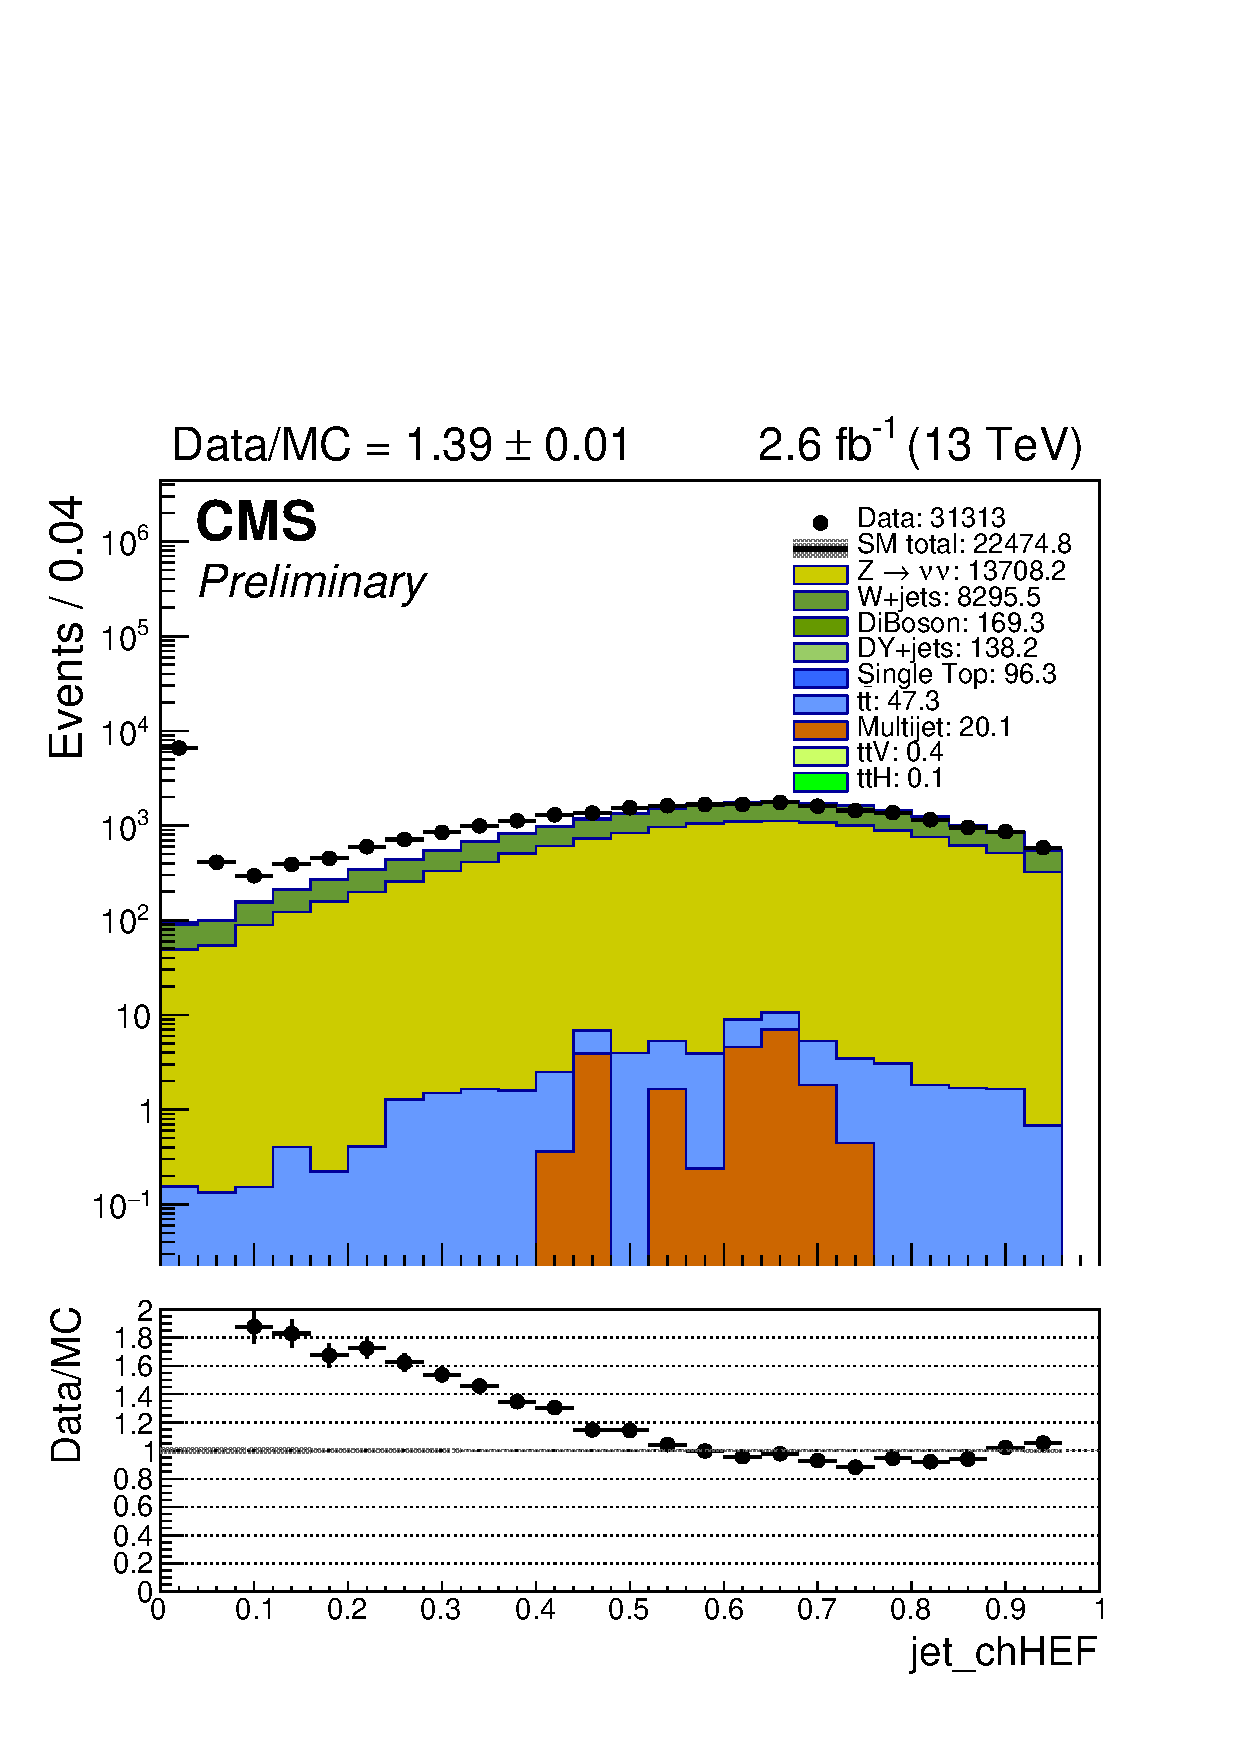
\includegraphics[width=0.32\textwidth]{figures/selection/jet_chHEF_mono_all_before.pdf}}
        {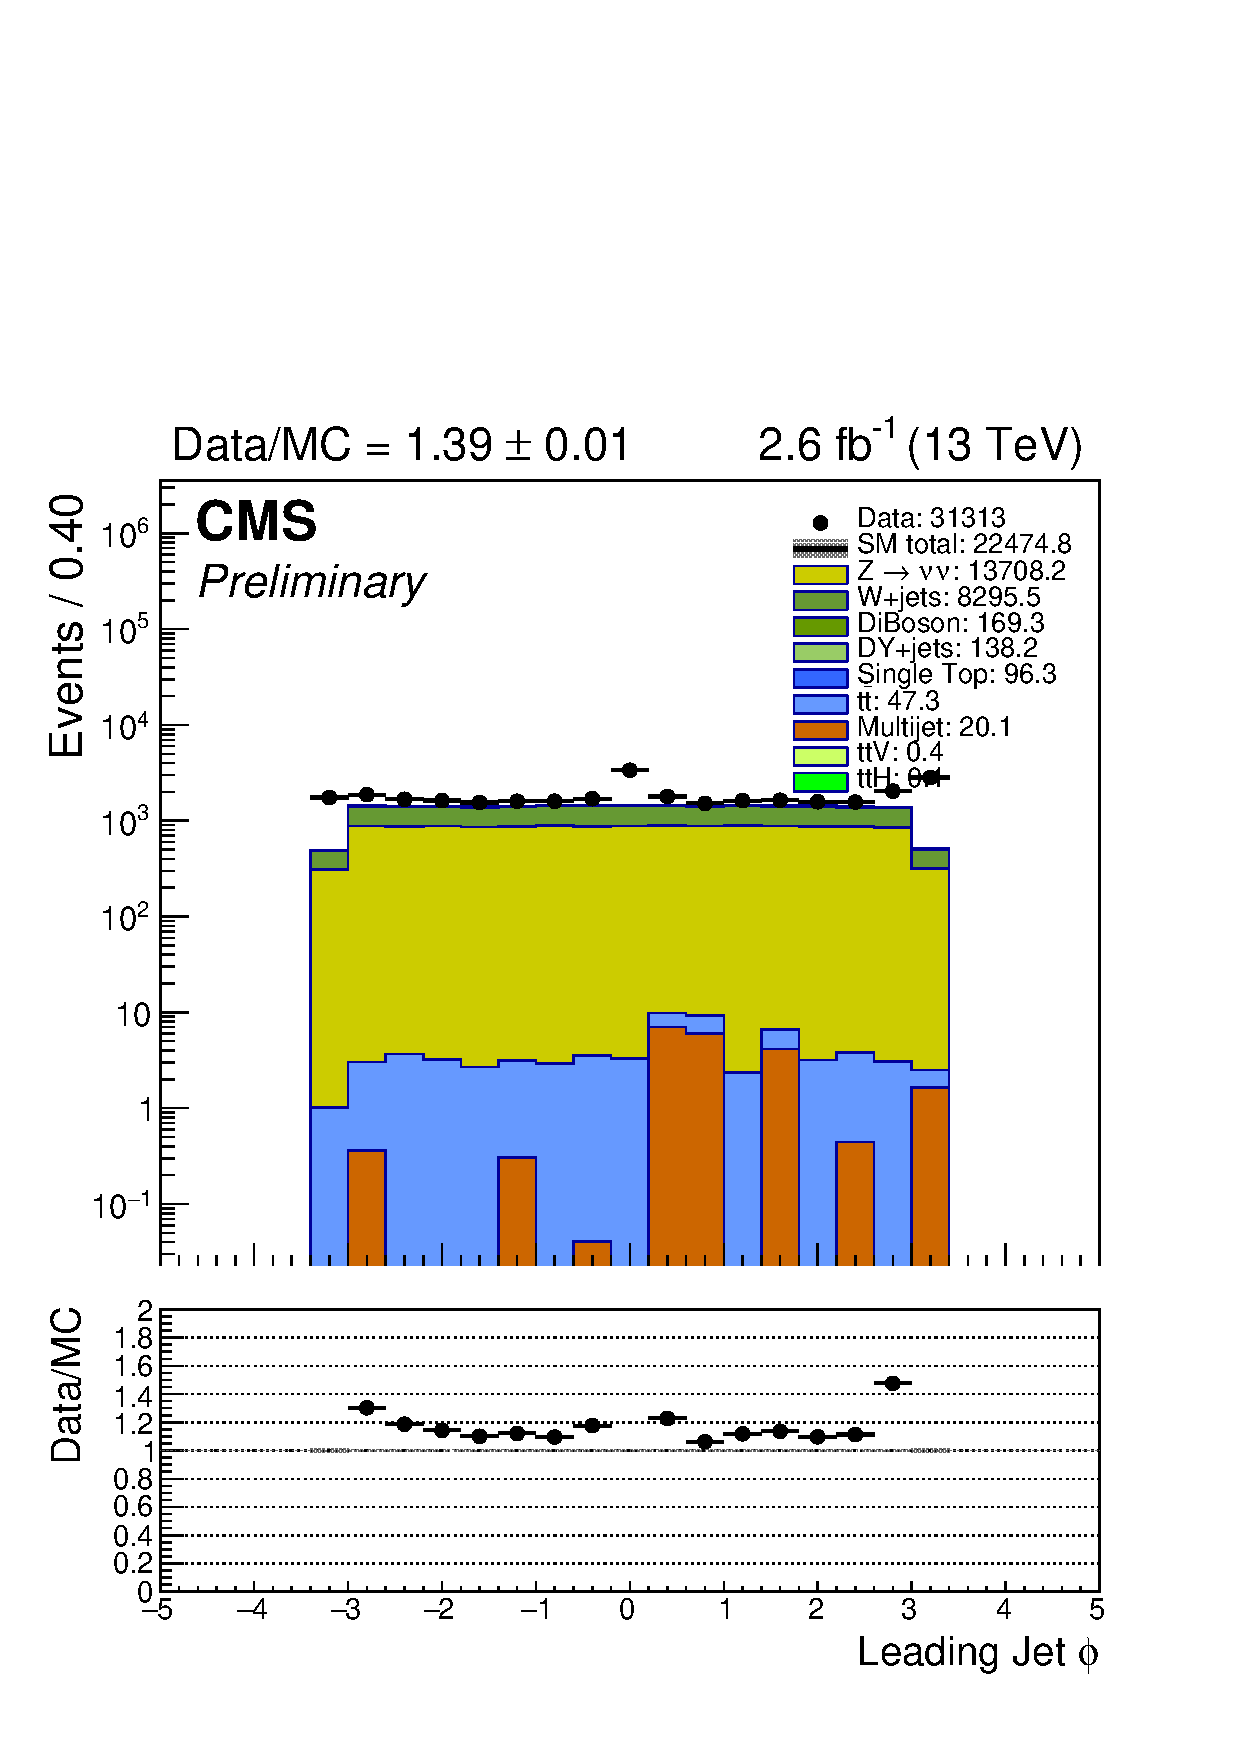
\includegraphics[width=0.32\textwidth]{figures/selection/jet_phi[0]_mono_all_before.pdf}}
        {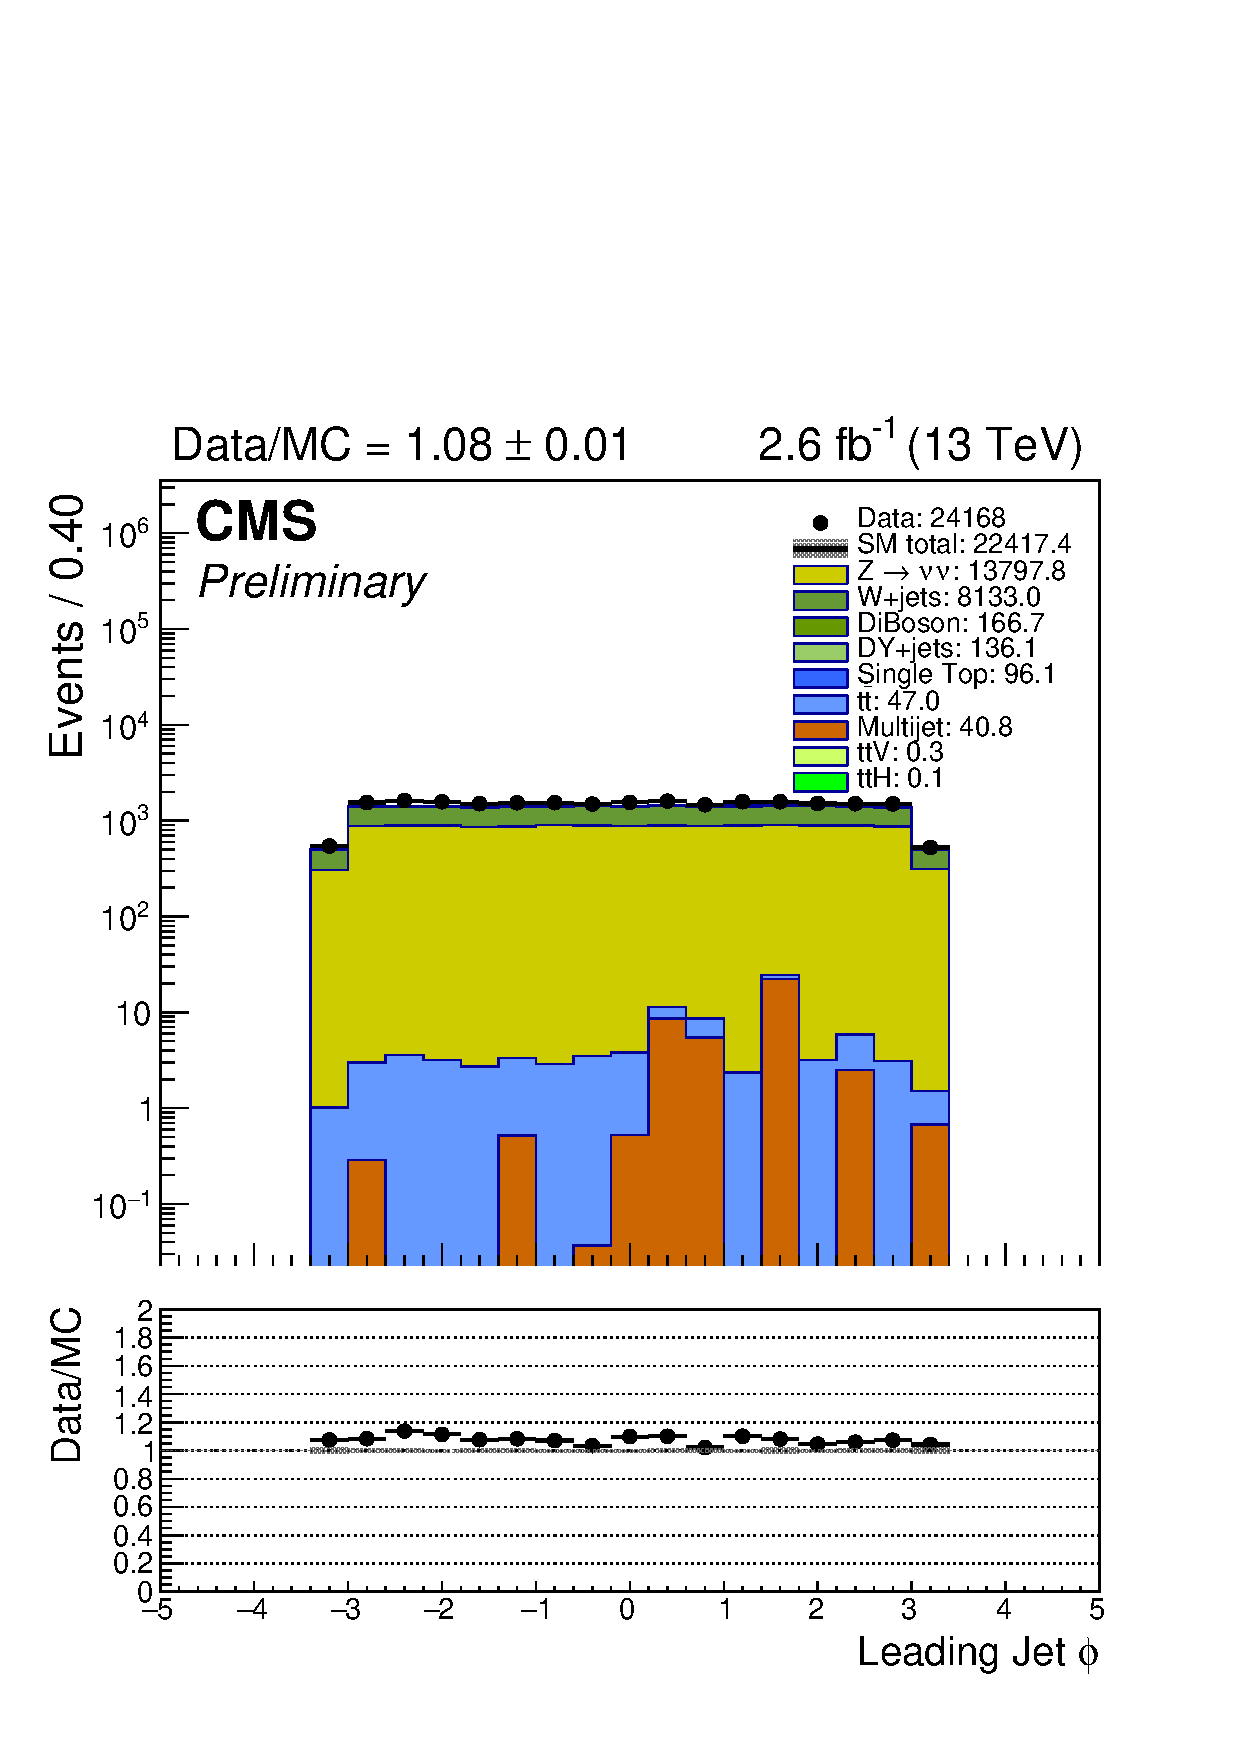
\includegraphics[width=0.32\textwidth]{figures/selection/jet_phi[0]_mono_all_after.pdf}}
        \caption{Distributions in the signal region of the jet charged hadron
        energy fraction (CHF) (Left), jet $\phi$ direction (Centre), and jet $\phi$
        direction after applying a requirement of {CHF~$>0.1$}. The large excess in data
        at charged hadron fractions close to zero and ${\phi = 0, \pi}$ is consistent with beam
        halo effects, and is effectively suppressed by the aforementioned selection.}
        \label{fig:leadJetCleaning}
    \end{center}
\end{figure}


\subsubsection{Summary of signal region selection} 
\label{sec:summary-selection}

The requirements that define the hadronic signal region are summarised
in Table~\ref{tab:sr-selections}.

\begin{table}[h!]
  \topcaption{Summary of the signal region selection criteria, applied
    in addition to the pre-selection summarised in
    Table~\ref{tab:pre-selections}.}
  \label{tab:sr-selections}
  \centering
  \footnotesize
  \begin{tabular}{ ll }
    \hline
    \hline
    Selection             & Requirement                                                    \\    
    \hline
    Veto                  & Veto on leptons, photons and SITs                              \\
    \alphat               & $>$0.52--0.65 (\HT-dependent) for region $200 < \HT < 900\gev$ \\
    \bdphi                & $>0.5$                                                         \\
    ``Beam Halo Filter''  &  $CHF(\textrm{leading jet})>0.1$                                \\
      &  $CHF(\textrm{leading jet})<0.95$                                \\
    \hline
    \hline
  \end{tabular}
\end{table}


\subsection{The control regions}
\label{sec:control-region-selection}


\subsubsection{The \texorpdfstring{\mj}{muon plus jets} control sample}
\label{sec:mucontrolSelection}

The selection criteria for the \mj sample are chosen to identify W
bosons decaying to a muon and a neutrino in the phase-space of the
signal. In order to select events containing W bosons, exactly one
tight isolated muon (defined in Sec.~\ref{sec:muon-id}) within an acceptance of \PT $>$ 30 \gev and
$|\eta| <$ 2.1 is required. The muons is removed from the event while computing the \met-based quantities, like \mht, \alphat. 
The transverse mass of the W candidate must satisfy $30 < \mt(\mu,\pfmet) < 125\gev$. 
This cut is also effective in reducing potential signal contamination 
for final states with leptons. 
Events are vetoed if $\Delta R(\mu,\textrm{jet}) < 0.5$ for at least one jet. 

Events are vetoed if well-reconstructed, isolated electrons and
photons, defined in Sec.~\ref{sec:objects}, are found to be within the
acceptances defined in Sec.~\ref{sec:vetoes}. Hence the vetoes mirror
exactly those used in the signal region, except for the selected
muon. Similarly, events containing single isolated tracks are also
vetoed according to the object and acceptance definitions found in
Secs.~\ref{sec:objects} and~\ref{sec:vetoes}. All single isolated
tracks in the event are considered, except for that associated with
the identified, isolated muon.

\subsubsection{The \texorpdfstring{\mmj}{di-muon plus jets} control sample}
\label{sec:mumucontrolSelection}

The selection criteria are identical to those for the \mj sample, with
the following exceptions that are tuned to identify Z bosons decaying
to two muons in the kinematic phase space of the signal region. 
In order to select an event sample containing Z bosons, exactly two
tight isolated muons (defined in Sec.~\ref{sec:muon-id}) within an acceptance of $\Pt > 30\gev$ and
$|\eta| < 2.1$ are required. The two muons are required to have opposite electric charge 
and the invariant mass of the two muons must satisfy $m_{Z} - 25 < M_{\mu_1\mu_2} < m_{Z} +25$. 
Events are vetoed if $\Delta R(\mu,\textrm{jet}) < 0.5$ is satisfied, running over all muons
and all jets. 

Events are vetoed if well-reconstructed, isolated electrons and
photons, defined in Sec.~\ref{sec:objects}, are found to be within the
acceptances defined in Sec.~\ref{sec:vetoes}. Hence the vetoes mirror
exactly those used in the signal region, except for the selected
muons. Similarly, events containing single isolated tracks are also
vetoed according to the object and acceptance definitions found in
Secs.~\ref{sec:objects} and~\ref{sec:vetoes}. All single isolated
tracks in the event are considered, except for that associated with
the identified, isolated muons.

\subsubsection{The \texorpdfstring{\gj}{photon plus jets} control sample}
\label{sec:photoncontrolSelection}

The \gj sample is defined by requiring exactly one photon (defined in Sec.~\ref{sec:photon-id}) satisfying
tight isolation criteria and within an acceptance of $\pt > 200\gev$
(limited by trigger requirements) and $|\eta| < 1.45$. Furthermore,
events are vetoed if $\Delta R(\gamma,\textrm{jet}) < 1.0$ is
satisfied for at least one jet. One important difference with
respect to the leptonic control samples is the application of the
\HT-dependent \alphat requirements imposed as part of the signal
region definition. This is done primarily to ensure that the photon
control sample and signal region are subject to identical kinematic
requirements and the photon carries sufficient transverse energy so
that the mass of the Z boson becomes a negligible effect when using
the \gj sample to predict the kinematic distributions of the \znunu
background. 

Events are vetoed if well-reconstructed, isolated muons and electrons,
defined in Sec.~\ref{sec:objects}, are found to be within the
acceptances defined in Sec.~\ref{sec:vetoes}. Hence the vetoes mirror
exactly those used in the signal region, except for the selected
photon. Similarly, events containing single isolated tracks are also
vetoed according to the object and acceptance definitions found in
Secs.~\ref{sec:objects} and~\ref{sec:vetoes}. 

\subsection{Event categorisation}
\label{sec:event-categorisation}

The events in the signal region and control regions are categorised according to 
\njet, \nb and \scalht. 
The categorisation in the control region ``mirrors'' the one in the search region: 
as a result no extrapolation is performed in these variables when predicting the backgrounds. \\
The bins used in the signal region are the result of an aggregation of the finer control region bins, 
with each of multiple control region bins predicting separately a category of events in the same aggregate bin in the signal region. 
This scheme, which is fully implemented in the likelihood as described in Sec. \ref{sec:likelihood}, allows 
to avoid any extrapolation while reducing the number of search categories. \\
The \textit{nominal} binning for these variables is summarised in Tab.~\ref{tab:nominal-binning}. 

\begin{table}[h!]
  \topcaption{Summary of the nominal \njet, \nb, \scalht binning.}
  \label{tab:nominal-binning}
  \centering
  \begin{tabular}{ cl }
    \hline
    \hline
    \multicolumn{2}{c}{Signal region} \\
    \hline
    Variable & Binning \\
    \hline
    \multirow{3}{*}{\njet}
     & Monojet:    $\njet=1$ \\
     & Asymmetric: $\njet \geq 2$ \\
     & Symmetric:  $\njet =2,3,4,5 \geq 6$ \\
    \hline
    \nb & $\nb=0,1,2,3,\geq 4$ \\
    \hline
    \scalht (GeV) & (200,400), (400,600), (600,900), (900,1200), $>$1200 \\
    \hline
    \hline
    \multicolumn{2}{c}{Control regions} \\
    \hline
    Variable & Binning \\
    \hline
    \multirow{3}{*}{\njet}
     & Monojet:    $\njet=1$ \\
     & Asymmetric: $\njet=2,3,4, \geq 5$ \\
     & Symmetric:  $\njet =2,3,4,5 \geq 6$ \\
    \hline
    \nb & $\nb=0,1,2,3,\geq 4$ \\
    \hline
    \scalht (GeV) & \parbox[t]{12cm}{(200,250), (250,300), (300,350), (350,400),
      (400,500), (500,600), \\ (600,750), (750,900), (900,1050), (1050,1200), $>$1200 } \\
    \hline
    \hline
  \end{tabular}
\end{table}


Starting from the definition of nominal binning, it has to be remarked that not all the (\njet,\nb,\scalht) combinations 
are kinematically accessible. For example, no $\njet=2,\nb=3$ bin exists (due to the jet multiplicity constraint) 
or $\njet^{sym} \geq 6,\scalht<400\,\mathrm{GeV}$ (due to jet acceptance requirements). 

Moreover, a requirement is made in order to ensure a reasonable number of events is available in data 
in each (\njet,\nb,\scalht) bin for the background prediction. 
A minimum of 10 events in every bin is required for at least one of the 3 control regions (\mj,\mmj,\gj). 

In order to improve the sensitivity to the signal, the search region is also binned in the \MHT dimension. 
Simulation mismodelling in this variable is reduced by binning the control regions finely in \scalht, i.e. by predicting 
events at the same ``scale''. A careful validation of the \MHT shape is carried out to assess 
the uncertainty in this extrapolation and it's described in Sec.~\ref{sec:syst-on-shape}. 

The \MHT templates which are used in the likelihood fit are built
using a minimum bin width of 100 GeV for $\MHT<400$ GeV and 200 GeV
above. The lowest nominal bin is $130<\MHT<200\,\mathrm{GeV}$. The
\MHT templates are naturally bounded from above by \scalht, apart from
the last open \scalht bin. However, the lower bound of the last open
bin is limited to $\MHT>1000\,\mathrm{GeV}$, to ensure sufficient data
counts in the control regions to validate the modelling at high \mht. 
Starting from this nominal binning, a requirement is made to ensure
that each bin in the template is well populated in the simulation.  At
least 100 unweighted MC events are required in each \njet,\scalht,\MHT
bin (inclusive in \nb). Adjacent \mht bins are merged until this
requirement is satisfied. 

The binning of the \MHT templates derived using these metrics is summarised in Tab.~\ref{tab:mht-binning}.


\newpage
\begin{table}[h!]
  \topcaption{Summary of the \MHT binning in each signal region
    category, determined according to the metrics described in this Section. The \MHT binning is identical in each \nb bin by construction.}
  \label{tab:mht-binning}
  \centering
  \begin{tabular}{ ccll }
    \hline
    \hline
    \njet & \nb & \scalht & \MHT \\
    \hline
    \multirow{4}{*}{$n_{\mathrm{jet}} = 1$} & \multirow{4}{*}{all} & [200,400] & [200,300], [300,inf] \\      
    & & [400,600] & [400,inf] \\ 
    & & [600,900] & [600,800], [800,inf] \\ 
    & & [900,inf] & [900,inf] \\     
    \hline
    \multirow{4}{*}{$n^{asym}_{\mathrm{jet}} \geq 2$} & \multirow{4}{*}{all} & [200,400] & [130,200], [200,300], [300,inf] \\
    & & [400,600] & [130,200], [200,300], [300,500], [500,inf] \\
    & & [600,900] & [130,400], [400,600], [600,800], [800,inf] \\
    & & [900,inf] & [130,800], [800,1000], [1000,inf] \\
    \hline
    \multirow{5}{*}{$n^{\mathrm{sym}}_{\mathrm{jet}} = 2$} & \multirow{5}{*}{all} & [200,400] & [130,200], [200,300], [300,inf] \\
    & & [400,600] & [130,200], [200,300], [300,500], [500,inf] \\
    & & [600,900] & [130,300], [300,400], [400,600], [600,800], [800,inf] \\
    & & [900,1200] & [130,300], [300,400], [400,600], [600,800], [800,1000], [1000,inf] \\
    & & [1200,inf] & [130,400], [400,600], [600,800], [800,1000], [1000,inf] \\
    \hline
    \multirow{5}{*}{$n^{\mathrm{sym}}_{\mathrm{jet}} = 3$} & \multirow{5}{*}{all} & [200,400] & [130,200], [200,300], [300,inf] \\    
    & & [400,600] & [130,200], [200,300], [300,500], [500,inf] \\
    & & [600,900] & [130,300], [300,500], [500,700], [700,inf] \\
    & & [900,1200] & [130,300], [300,400], [400,600], [600,800], [800,1000], [1000,inf] \\
    & & [1200,inf] & [130,400], [400,600], [600,800], [800,1000], [1000,inf] \\
    \hline
    \multirow{5}{*}{$n^{\mathrm{sym}}_{\mathrm{jet}} = 4$} & \multirow{5}{*}{all} & [200,400] & [130,200], [200,300], [300,inf] \\
    & & [400,600] & [130,200], [200,300], [300,500], [500,inf] \\
    & & [600,900] & [130,200], [200,300], [300,500], [500,700], [700,inf] \\
    & & [900,1200] & [130,300], [300,400], [400,600], [600,800], [800,1000], [1000,inf] \\
    & & [1200,inf] & [130,300], [300,400], [400,600], [600,800], [800,1000], [1000,inf] \\
    \hline
    \multirow{5}{*}{$n^{\mathrm{sym}}_{\mathrm{jet}} = 5$} & \multirow{5}{*}{all} & [200,400] & [130,200], [200,inf] \\
    & & [400,600] & [130,200], [200,300], [300,400], [400,inf] \\
    & & [600,900] & [130,300], [300,500], [500,700], [700,inf] \\
    & & [900,1200] & [130,300], [300,500], [500,700], [700,900], [900,inf] \\
    & & [1200,inf] & [130,300], [300,400], [400,600], [600,800], [800,1000], [1000,inf] \\
    \hline
    \multirow{4}{*}{$n^{\mathrm{sym}}_{\mathrm{jet}} \geq 6$} & \multirow{4}{*}{all} & [400,600] & [130,200], [200,300], [300,inf] \\
    & & [600,900] & [130,300], [300,400], [400,600], [600,inf] \\
    & & [900,1200] & [130,200], [200,300], [300,400], [400,600], [600,800], [800,inf] \\
    & & [1200,inf] & [130,300], [300,400], [400,600], [600,1000], [1000,inf] \\
    \hline
    \hline
  \end{tabular}
\end{table}

%\section{The ``b-tag formula method''}
\label{sec:formula}

In order to maximise sensitivity to potential new physics signatures
in final states with multiple b-quark jets, a method that improves the
statistical power of the simulation, particularly for high btag bins, is
employed. This method is known as the ``formula'' method. The
resulting improvement in the statistical precision of the simulation
propagates through to the transfer factors used in the analysis.

\subsection{Method}
\label{sec:formula-method}

The distribution of the number of bjets (\nb) is estimated from generator-level information
contained in the simulation. The number of reconstruction-level jets
matched to underlying bottom quarks ($\nb^{\rm gen}$), charm quarks
($n_{\rm c}^{\rm gen}$), and light-flavoured partons, i.e. $u,d,s$ quarks and gluons ($n_{\rm
  l}^{\rm gen}$) per event, $N(\nb^{\rm gen},n_{\rm c}^{\rm
  gen},n_{\rm l}^{\rm gen})$, is recorded in bins of (\njet
   , \scalht, \mht). 
 The matching between truth-level partons
and reconstruction-level jets is achieved with a matching algorithm
recommended by the BTV POG~\cite{btagMCTools}.
 The b-tagging efficiency, $\epsilon_{\rm b}$, and mistag probabilities,
$\epsilon_{\rm c}$ and $\epsilon_{\rm l}$, are also determined from simulation
in bins of (\njet,~\scalht,~\mht), with each quantity averaged
over jet $p_{\rm T}$ and $\eta$. Corrections are applied on a
jet-by-jet basis to both $\epsilon_{\rm b}$, $\epsilon_{\rm c}$, and $\epsilon_{\rm l}$
in order to match the corresponding measurements from
data. These corrections, or ``scale factors'', are provided by the BTV POG~\cite{btagMCTools}.

The above information is sufficient to predict the total number of b-tagged jets in the event $n^{\rm tag} \equiv n_{\rm b}^{\rm tag} + n_{\rm c}^{\rm tag} + n_{\rm l}^{\rm tag}$ and thus also
determine the event yield $N(n^{\rm tag})$ from simulation for a given
bin in (\njet,~\scalht,~\mht) with the expression:

\begin{equation}
  \label{equ:btag-formula}
  N(n^{\rm tag}) = \sum_{n_{i}^{\rm gen}} N(n_{\rm b}^{\rm gen},n_{\rm c}^{\rm gen},n_{\rm l}^{\rm gen}) \times (\sum_{n_{i}^{\rm tag}}P_{\rm b}\times P_{\rm c} \times P_{\rm l})
\end{equation}

where $n_{\rm b}^{\rm tag}$, $n_{\rm c}^{\rm tag}$ and $n_{\rm l}^{\rm tag}$ are the number of reconstructed and b-tagged jets 
which are matched to a $b,c$ and $l$ quark respectively and 
$P_{i} = P_{\mathrm{binomial}}(n_{i}^{\rm tag}; n_{i}^{\rm gen}, \epsilon_{i})$ is the usual binomial probability density.

As a simple example, consider a bin with 2 reconstructed jets, in which 
1000 events contain 2 light-jets, i.e. $(n_{\rm b}^{\rm gen} = 0,n_{\rm c}^{\rm gen} = 0,n_{\rm l}^{\rm gen} = 2)$ and 
500 events contain 1 light-jet and 1 b-jet, i.e. $(n_{\rm b}^{\rm gen} = 1,n_{\rm c}^{\rm gen} = 0,n_{\rm l}^{\rm gen} = 1)$. 
In this exercise, we assume a b-tag efficiency $\epsilon_{\rm b} = 0.65$ and a light-tag efficiency $\epsilon_{\rm l} = 0.01$. 
The MC yields for the 3 b-tag multiplicities are then calculated as follows:

\begin{align*}
%% \begin{split}
N(0) &= 1000\times (1-\epsilon_{\rm l})^2 \\
     &+ 500\times (1-\epsilon_{\rm b})\times(1-\epsilon_{\rm l}) = 1153.35 \\
N(1) &= 1000\times (1-\epsilon_{\rm l})\times \epsilon_{\rm l} \times 2 \\
     &+ 500\times (1-\epsilon_{\rm b})\times\epsilon_{\rm l} \\
     &+ 500\times \epsilon_{\rm b} \times (1-\epsilon_{\rm l})\times = 343.3 \\
N(2) &= 1000\times \epsilon_{\rm l}^2 \\
     &+ 500\times \epsilon_{\rm b} \times \epsilon_{\rm l} = 3.35 \\
%% \end{split}
\end{align*}

  
The method exploits the ability to make precise measurements of
$N(n_{\rm b}^{\rm gen},n_{\rm c}^{\rm gen},n_{\rm l}^{\rm gen})$,
$\epsilon$, $f_{\rm c}$, and $f_{\rm l}$ independently of $n_{\rm
  b}$, which means that event yields for a given b-quark jet
multiplicity can be predicted with a higher statistical precision than
obtained directly from simulation. Precise measurements of $f_{\rm c}$
and $f_{\rm l}$ are particularly important for events with $n_{\rm
  b} \geq 3$, which often occur in the SM because of the presence of
mistagged jets in the event. In this case, the largest background is
\ttbar, with two correctly tagged b-quark jets and an additional
mistagged jet originating from a charm quark or light-flavoured
parton.

\subsection{Validation}
\label{sec:formula-validation}

Predictions from the formula method are used to construct transfer 
factors as described in Section~\ref{sec:backgroundmet} and \mht templates 
as described in Section~\ref{sec:syst-on-shape}. 
In order to validate the implementation of the method 
a closure test is performed where the predictions from the formula method 
are compared to the ones from the ``vanilla'' MC, for every 
(\njet,\scalht,\mht) bin. \\
%% As an additional check, the same closure test is performed using the loose b-tag working point. \\ %FIXME: don't have the plots right now
The results in terms of pulls are presented in Fig.~\ref{fig:formula-validation-singlemu} for the \mj control region. 
A good closure is observed which validates the method and its implementation.

The same kind of closure test is carried out at the transfer factor level \ref{sec:backgroundmet}. %FIXME: fix ref 
Additionally, the check is performed for the ``loose'' and ``tight'' working point of the b-tag discriminator, 
beside the ``medium'', which is used in the analysis. \\
The results of this validation is shown in Fig.~\ref{fig:formula-validation-TF}. 
A good closure is observed also in this case. 

\begin{figure}[h!]
  \centering
  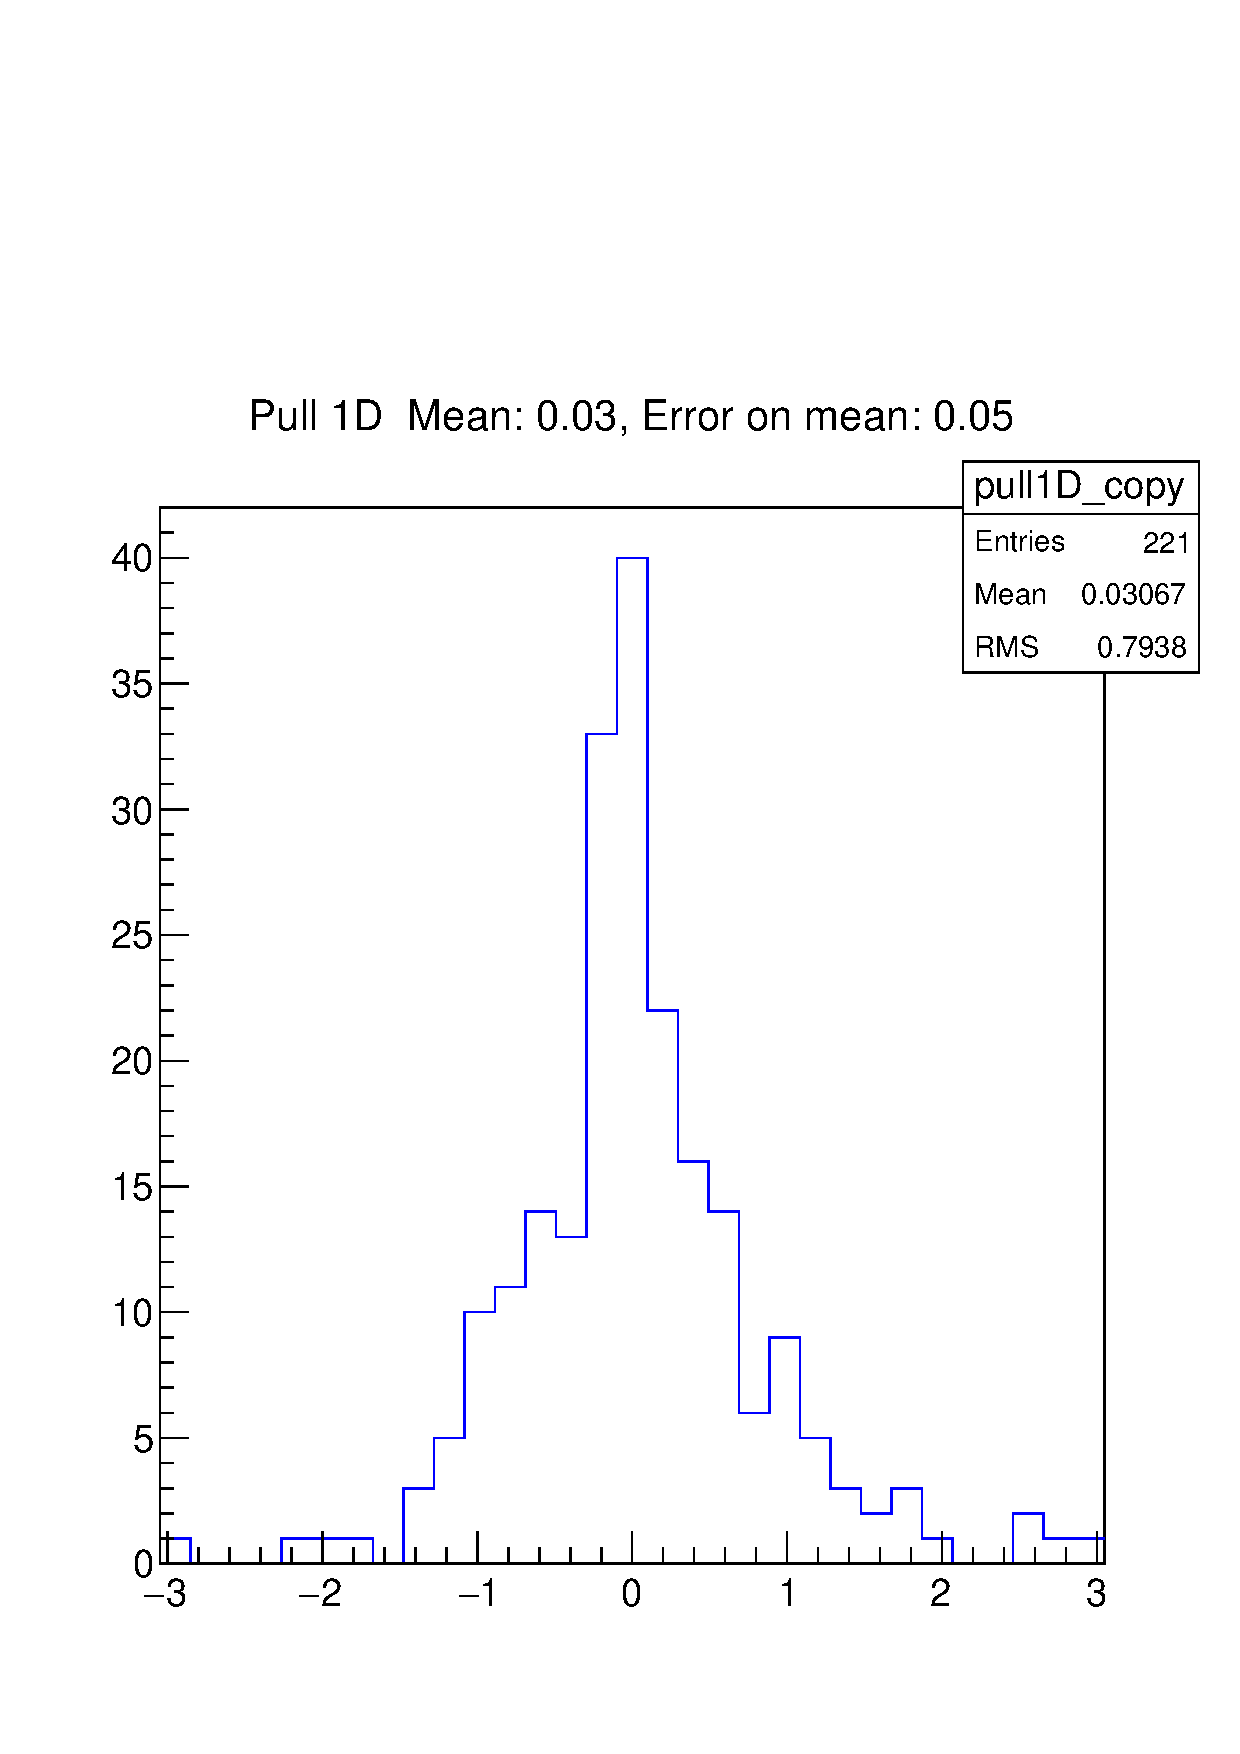
\includegraphics[width=0.45\textwidth]{figures/btagformula/validation/ValidationSingleMu}~
  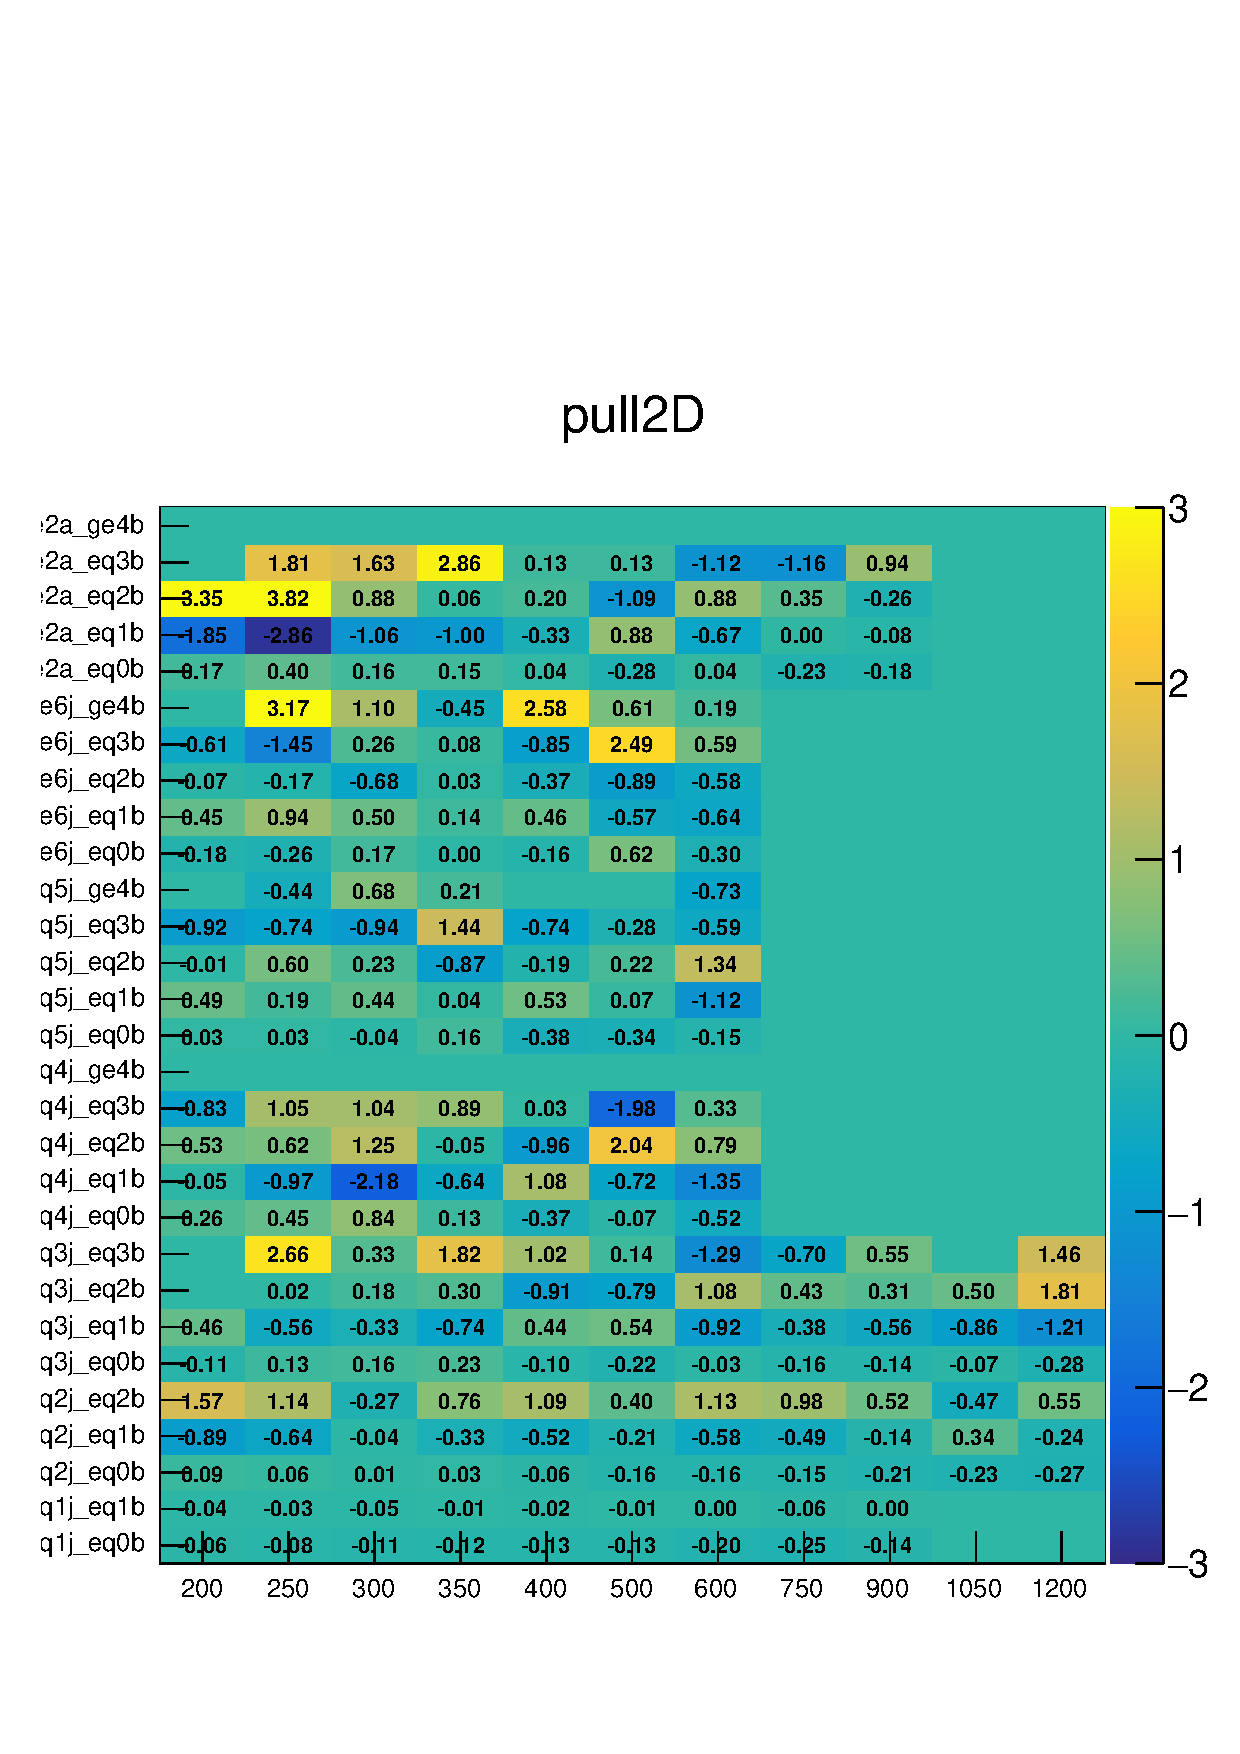
\includegraphics[width=0.45\textwidth]{figures/btagformula/validation/ValidationSingleMu2D} \\
  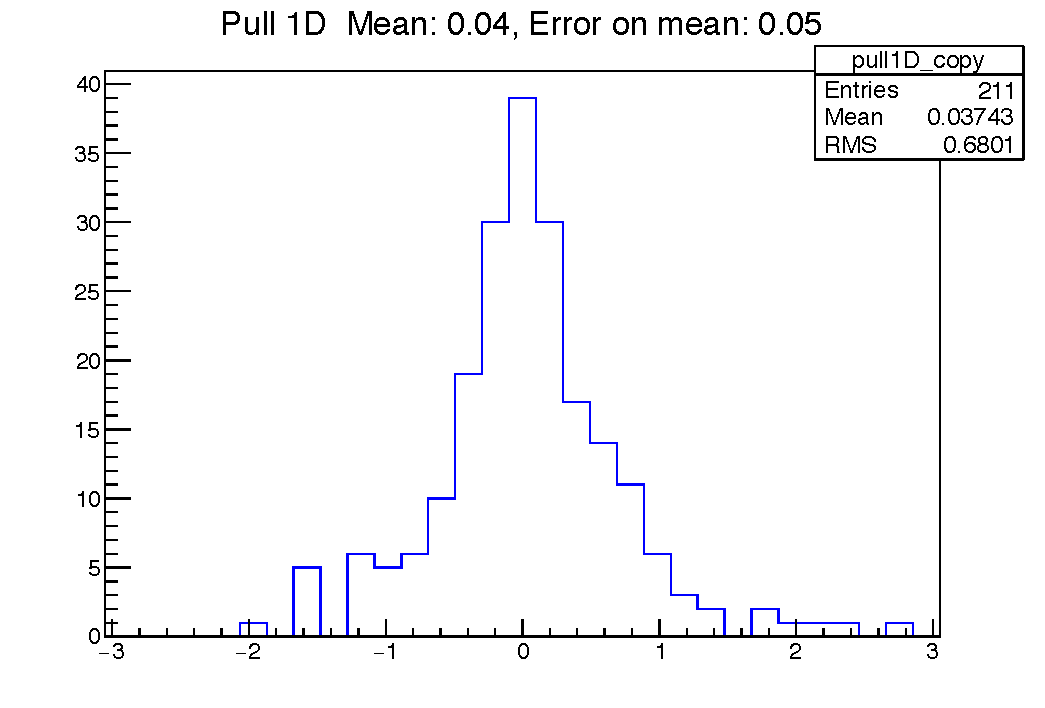
\includegraphics[width=0.45\textwidth]{figures/btagformula/validation/ValidationTTJets}~
  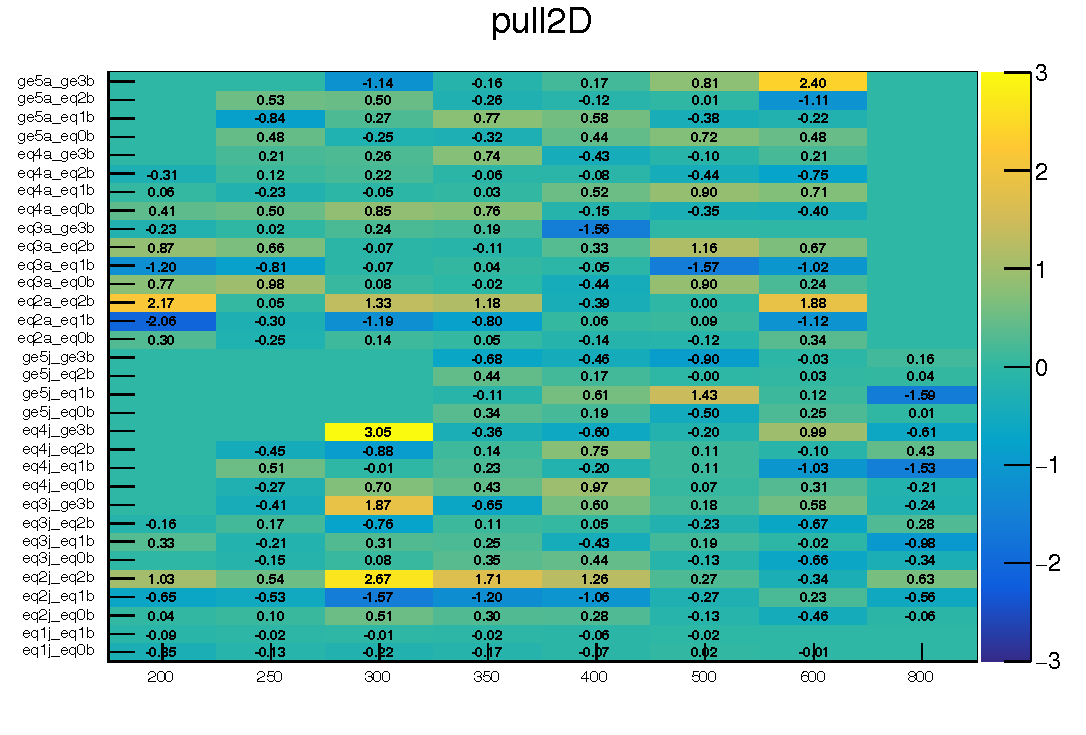
\includegraphics[width=0.45\textwidth]{figures/btagformula/validation/ValidationTTJets2D} \\
  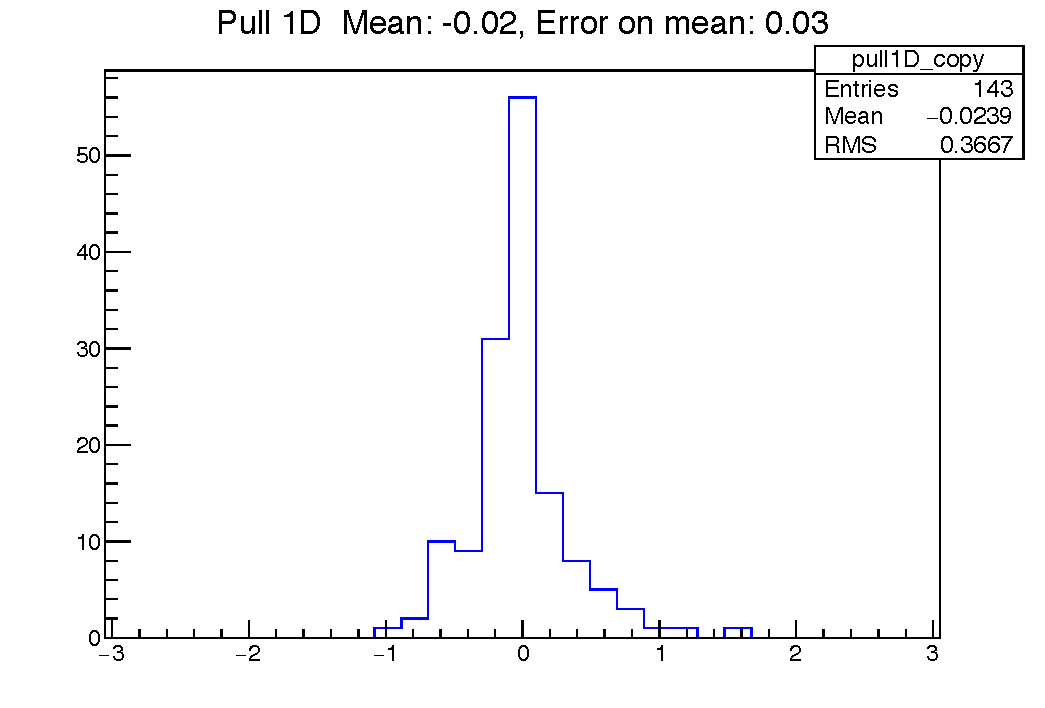
\includegraphics[width=0.45\textwidth]{figures/btagformula/validation/ValidationWJets}~
  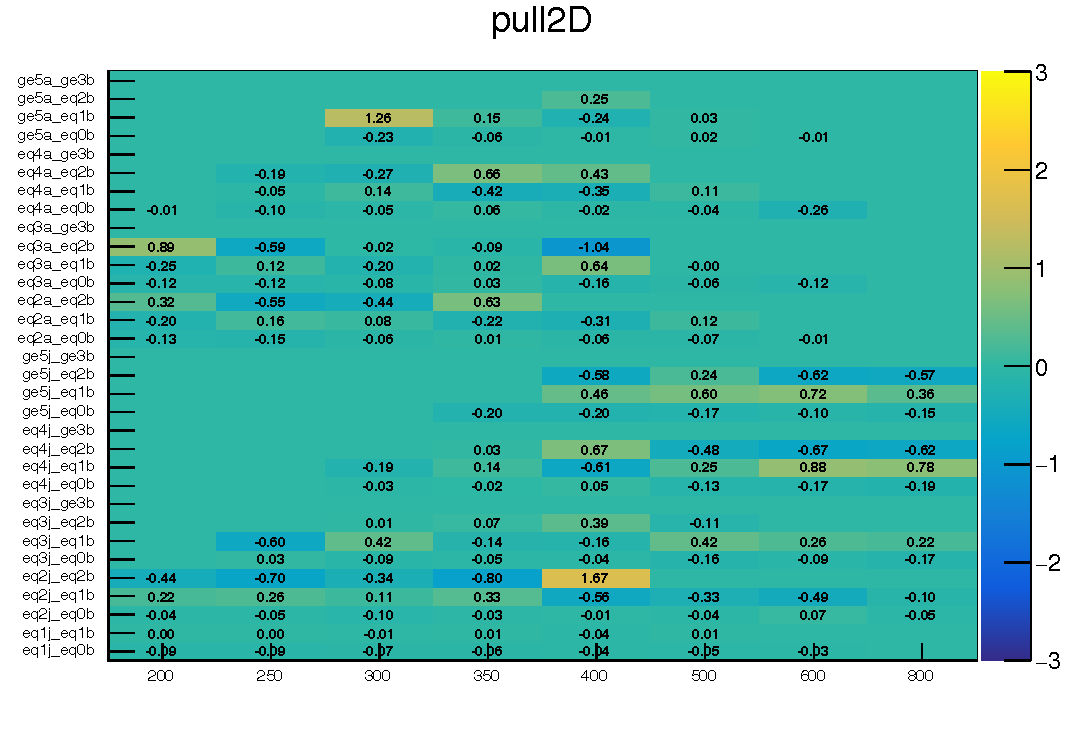
\includegraphics[width=0.45\textwidth]{figures/btagformula/validation/ValidationWJets2D} \\
  \caption{\label{fig:formula-validation-singlemu}
  Inclusive pull distribution (left) and 2D pull distribution as a function of \scalht and (\njet,\nb) bin (right) for
  the total \mj control region yields (top), only the TTJets yields (middle) and only the WJets yields (bottom).
  The pull is defined as the vanilla MC prediction minus the formula method prediction divided by the statistical uncertainty. }
\end{figure}


\begin{figure}[h!]
  \centering
  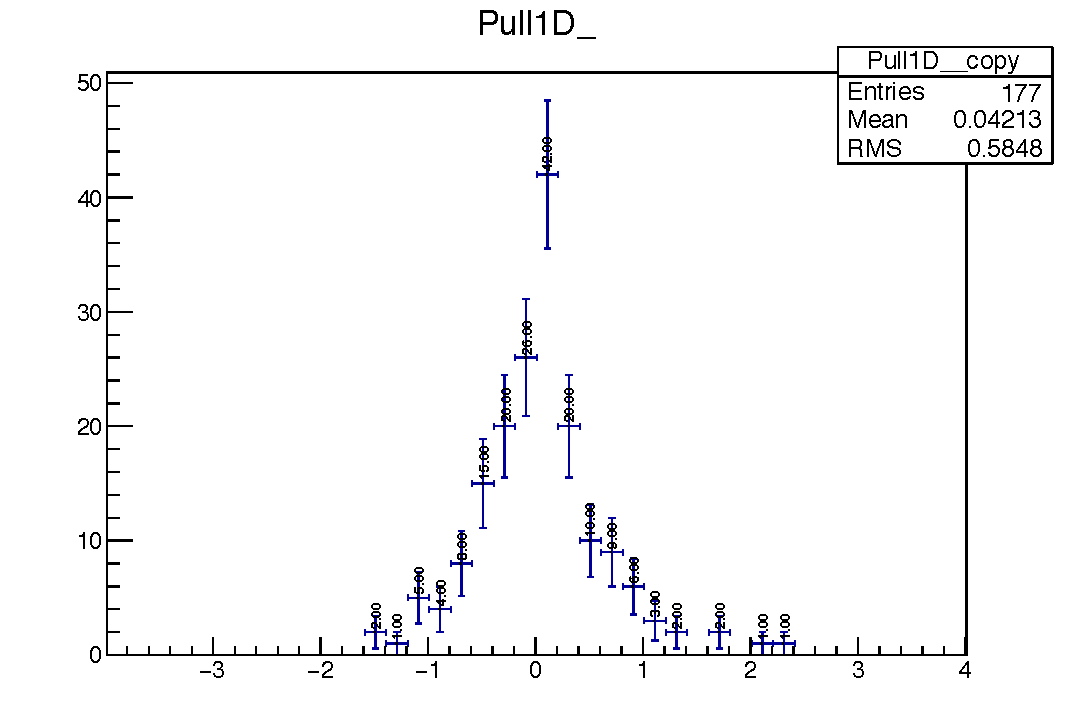
\includegraphics[width=0.45\textwidth]{figures/btagformula/validation/TFValidationSingleMu_loose}~
  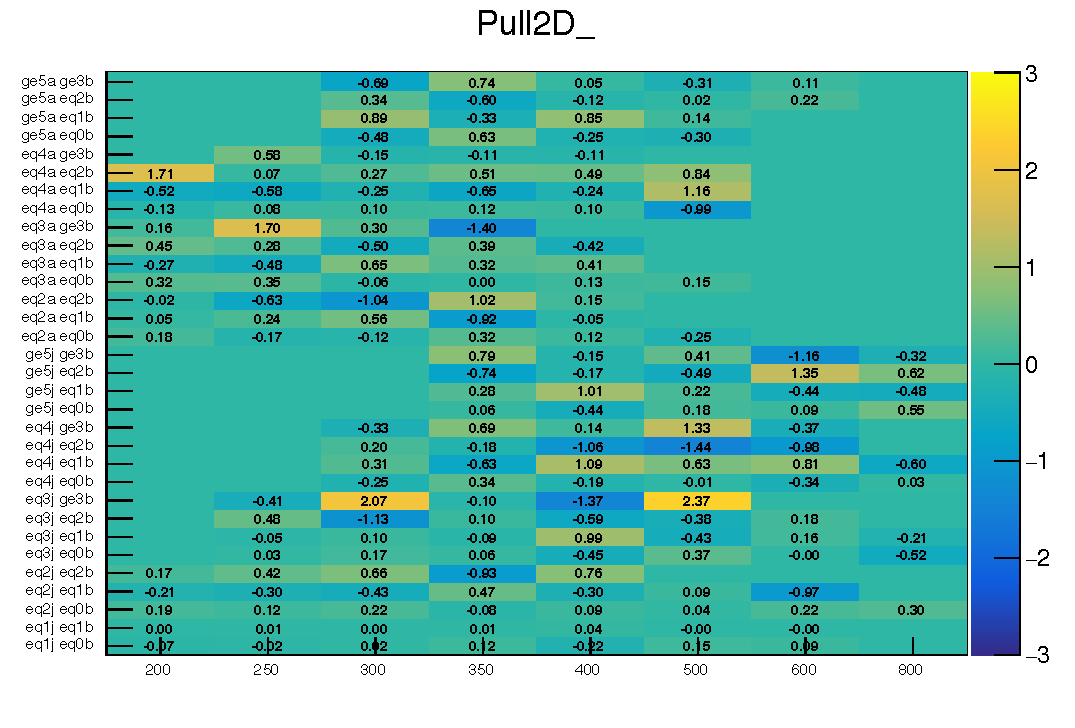
\includegraphics[width=0.45\textwidth]{figures/btagformula/validation/TFValidation2DSingleMu_loose} \\
  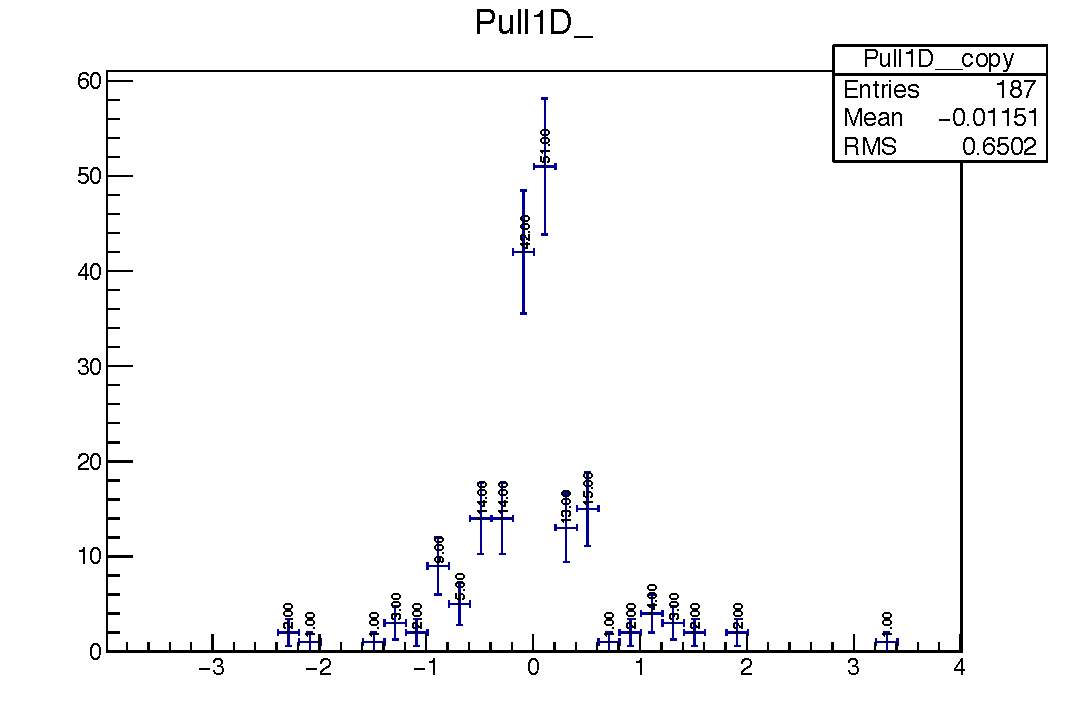
\includegraphics[width=0.45\textwidth]{figures/btagformula/validation/TFValidationSingleMu_medium}~
  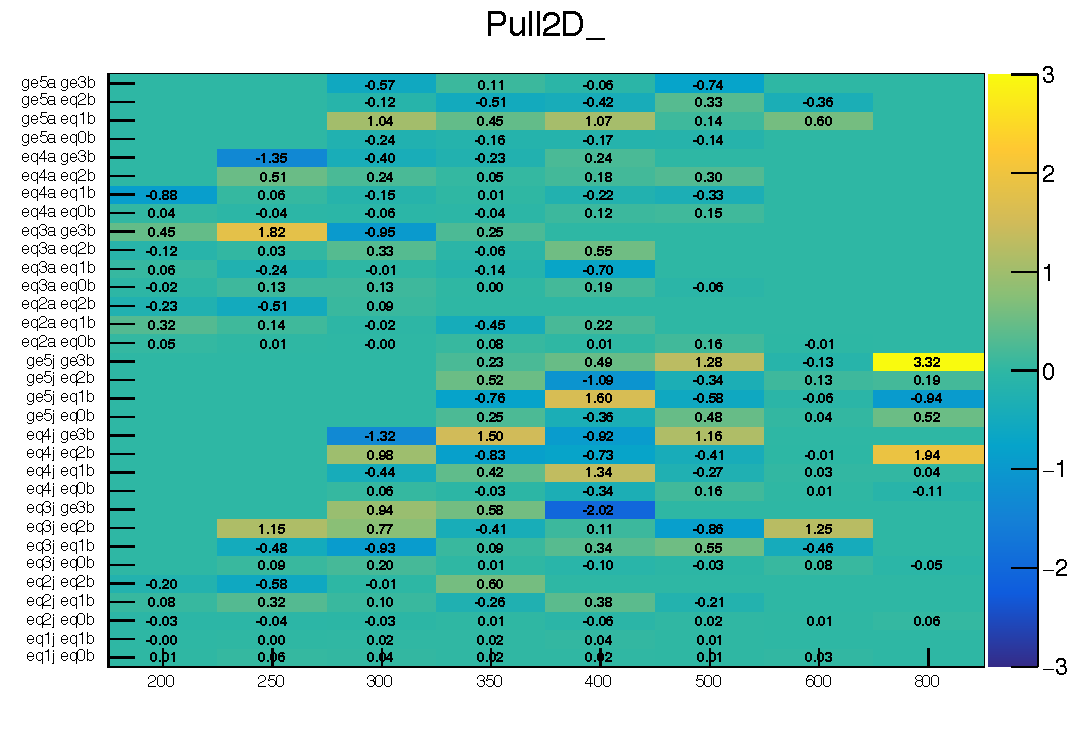
\includegraphics[width=0.45\textwidth]{figures/btagformula/validation/TFValidation2DSingleMu_medium} \\
  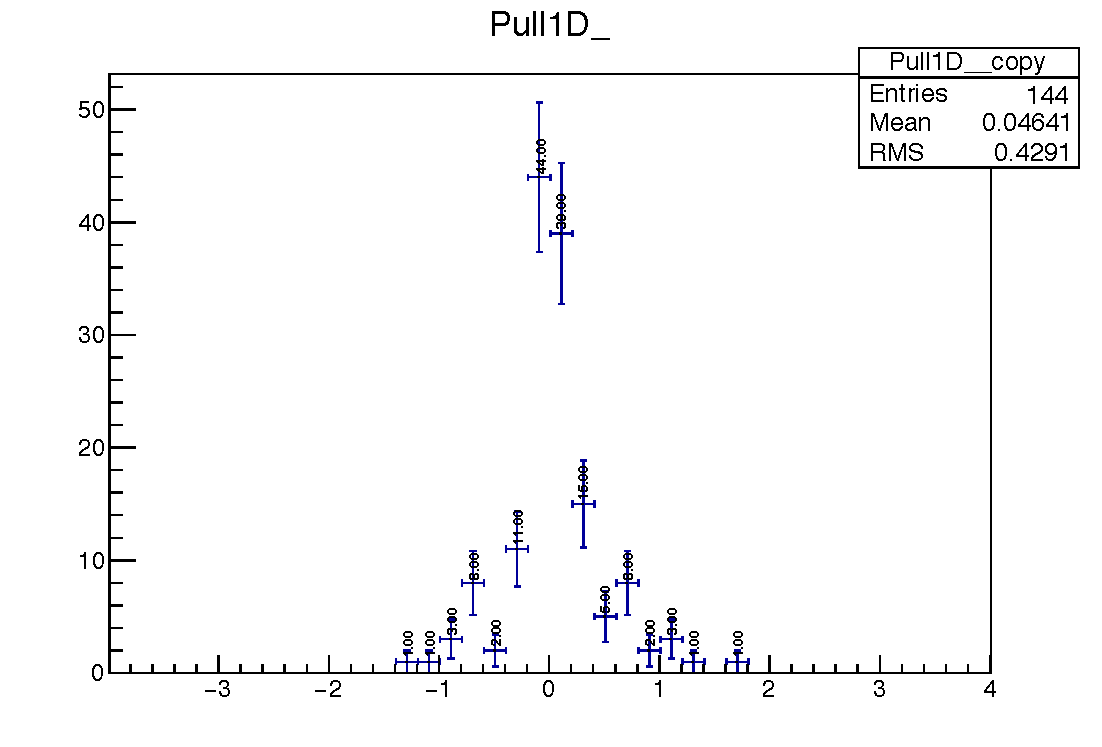
\includegraphics[width=0.45\textwidth]{figures/btagformula/validation/TFValidationSingleMu_tight}~
  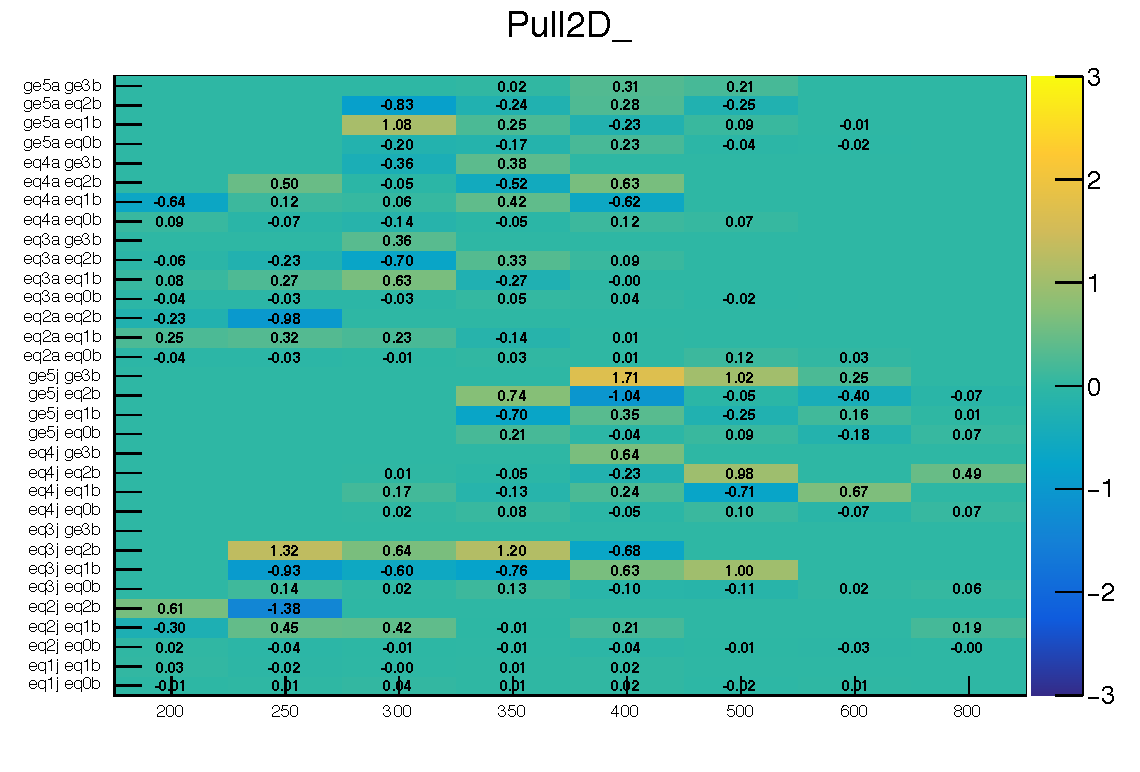
\includegraphics[width=0.45\textwidth]{figures/btagformula/validation/TFValidation2DSingleMu_tight} \\
  \caption{\label{fig:formula-validation-TF}
  Inclusive pull distribution (left) and 2D pull distribution as a function of \scalht and (\njet,\nb) bin (right) for
  the \mj transfer factor (TF) using the loose (top) the medium (middle) and the tight (bottom) working point of the b-tag discriminator. 
  The pull is defined as the vanilla MC TF minus the formula method TF divided by the statistical uncertainty. }
\end{figure}



\subsection{Uncertainties on the predicted MC yields}
\label{sec:formula-uncertainties}
The uncertainties on the MC yields predicted by the b-tag formula method, described in Sec.~\ref{sec:formula-method}, 
are derived by means of a toy procedure. 
A set of 1000 toys is generated randomising the inputs to the method. 
In each toy the $n^{\rm tag}$ distribution is computed after randomising 
the gen-level flavour configuration $N(n_{\rm b}^{\rm gen},n_{\rm c}^{\rm gen},n_{\rm l}^{\rm gen})$ 
from a Poisson statistics and the b-tag efficiencies $\epsilon_{i}$ ($i=\rm b,\rm c,\rm l$) using a Gaussian probability density function. 
The covariance matrix for the $n^{\rm tag}$ bins is then extracted in each (\njet,\scalht,\mht) category and diagonalised. 
From the diagonal terms of this matrix up to 5 un-correlated $n^{\rm tag}$ templates are derived, 
depending on the jet multiplicity in each bin. 
These templates, encoding the uncertainty in the event yield predictions with the b-tag formula method, 
are implemented in the likelihood fit as alternative shapes. 
The uncertainties derived using this procedure effectively replace the bin-by-bin MC statistical uncertainty 
used in the previous iteration of the analysis. 

Fig.~\ref{fig:formula-uncertainties} shows the nominal $n^{\rm tag}$ template and the alternative shapes derived with 
the toy procedure described in this section. 
The statistical uncertainty from the vanilla MC is also shown for comparison. 
From these figures the improvement in the precision of the yield prediction using the formula method can be fully appreciated. 

\begin{figure}[h!]
  \centering
  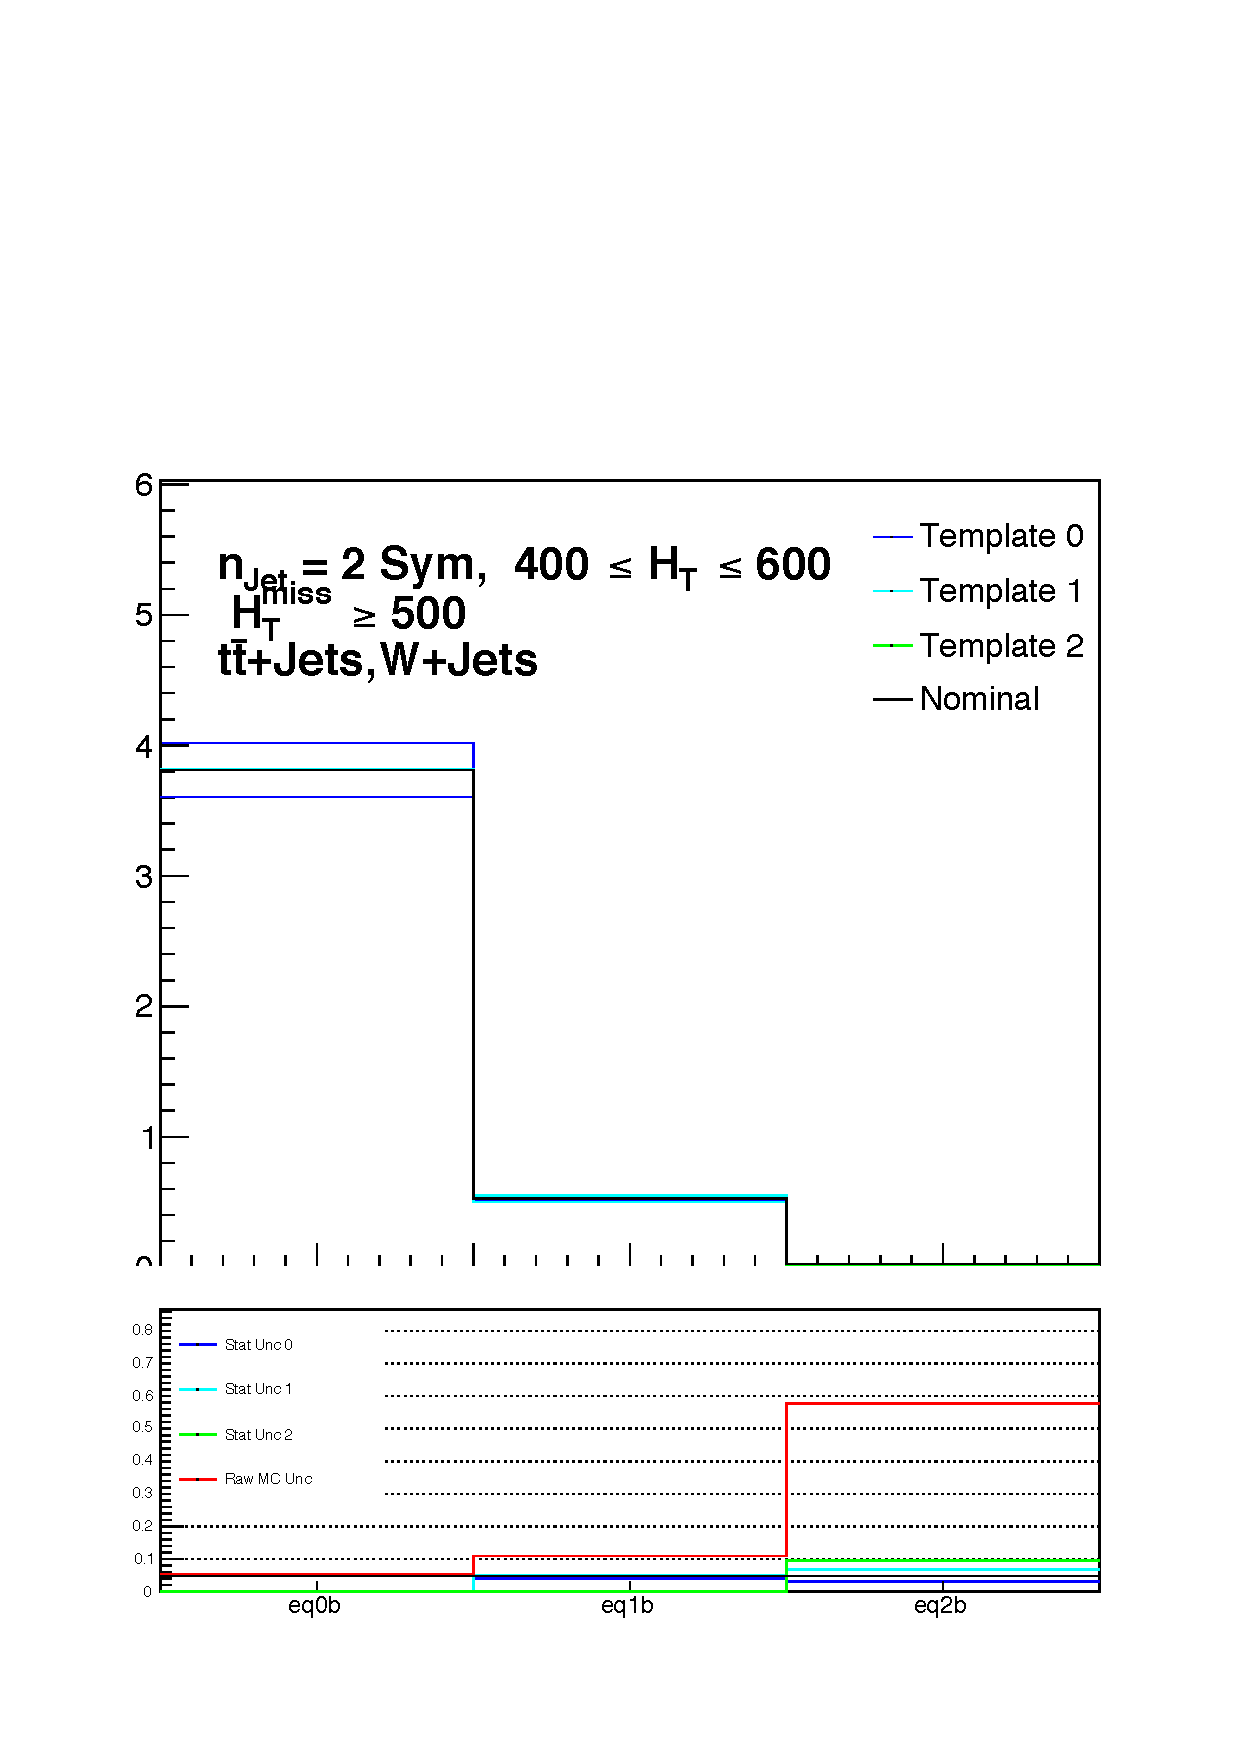
\includegraphics[width=0.45\textwidth]{figures/btagformula/uncertainties/Ttw_eq2j_400600_500Inc}~
  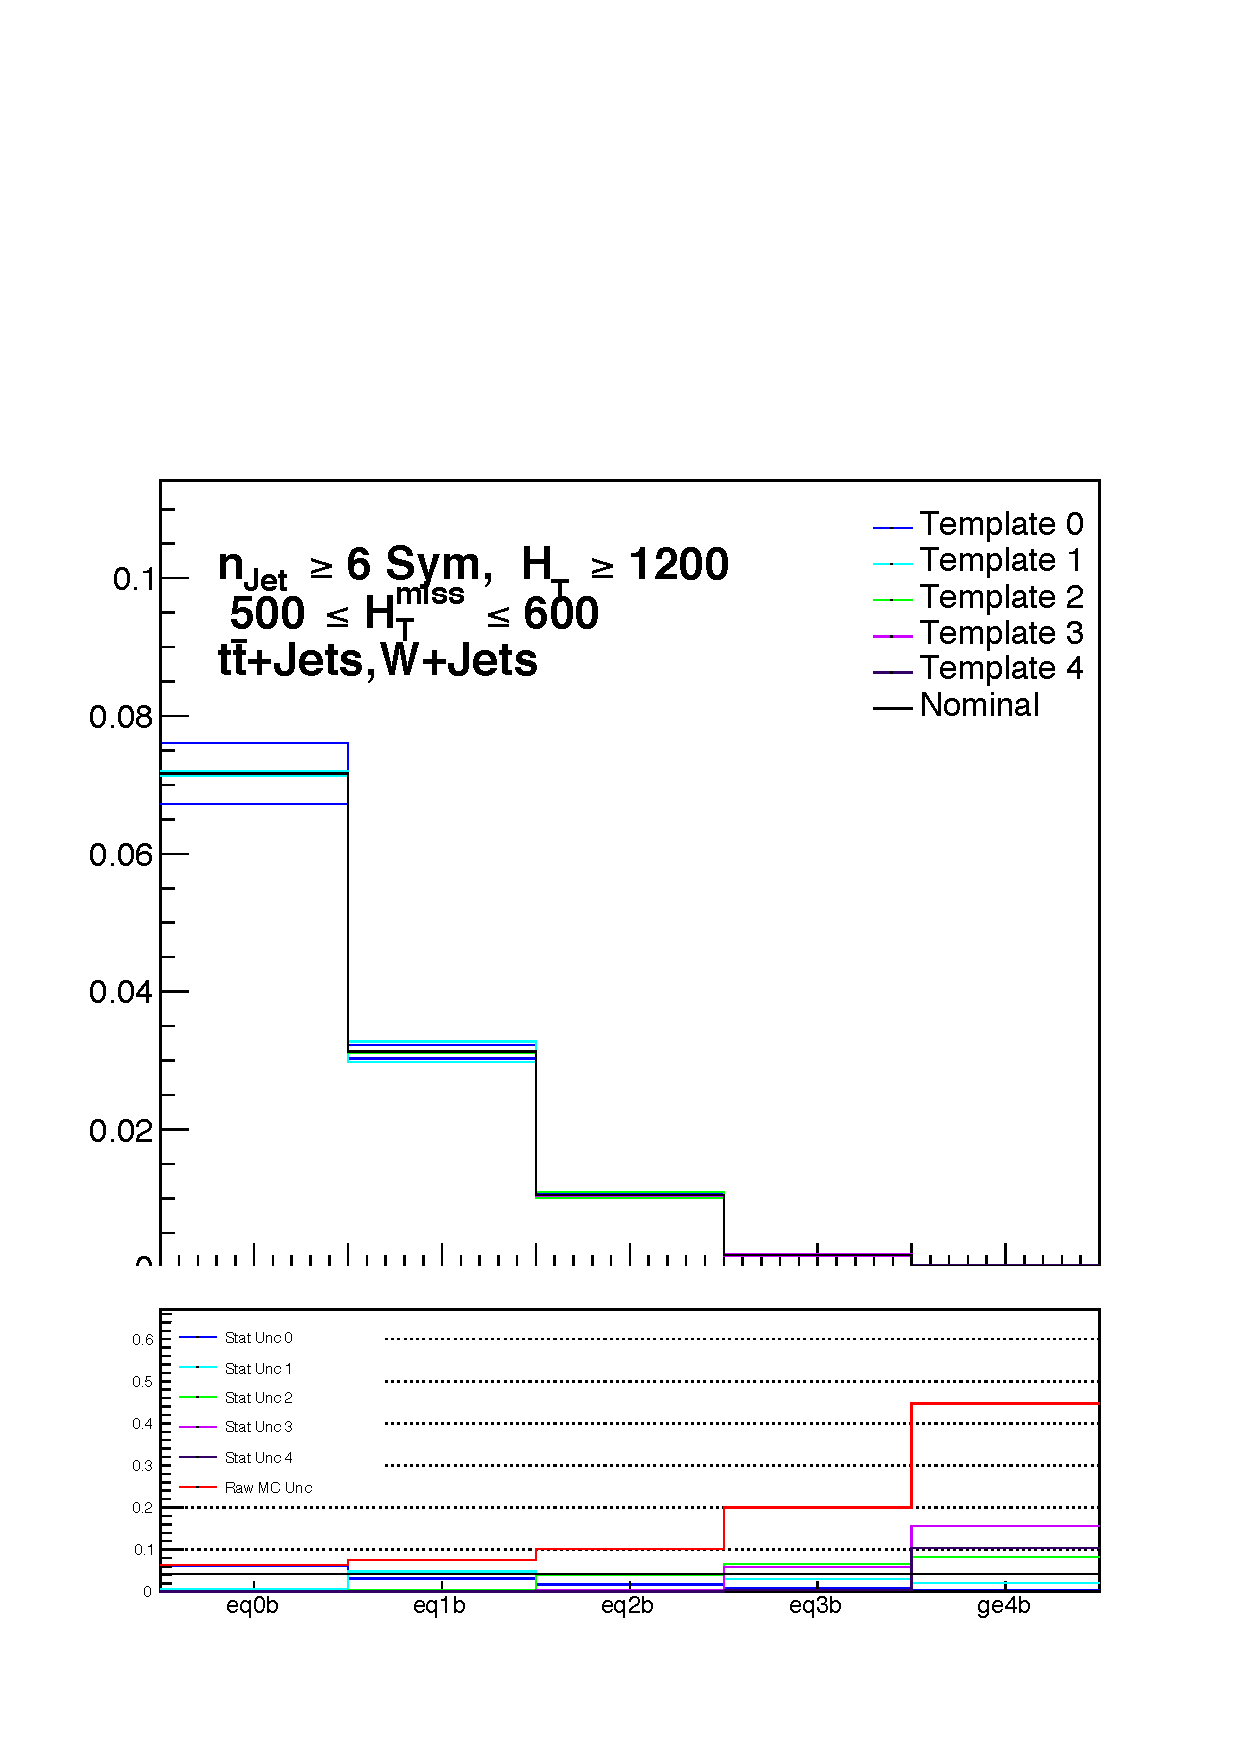
\includegraphics[width=0.45\textwidth]{figures/btagformula/uncertainties/Ttw_ge6j_1200Inc_500600} \\
  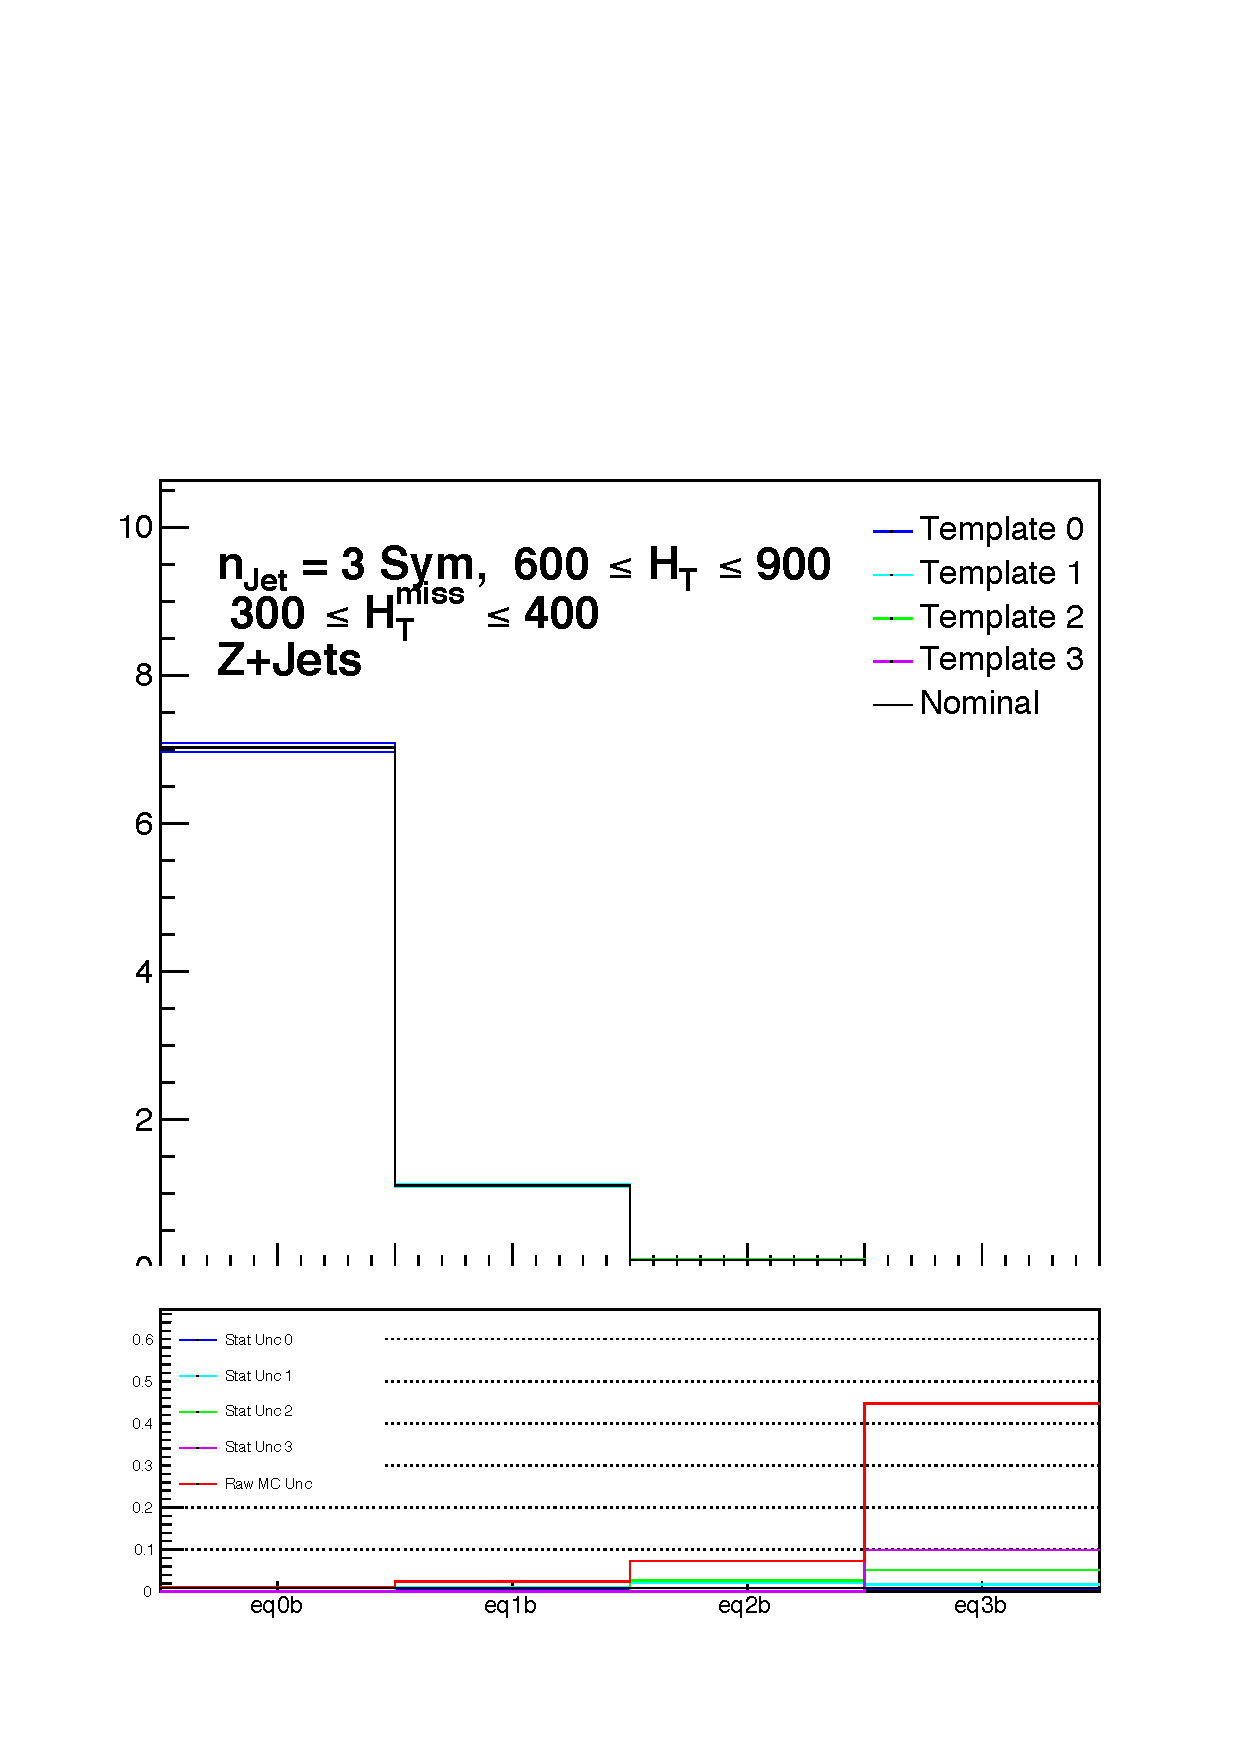
\includegraphics[width=0.45\textwidth]{figures/btagformula/uncertainties/Zinv_eq3j_600900_300400}~
  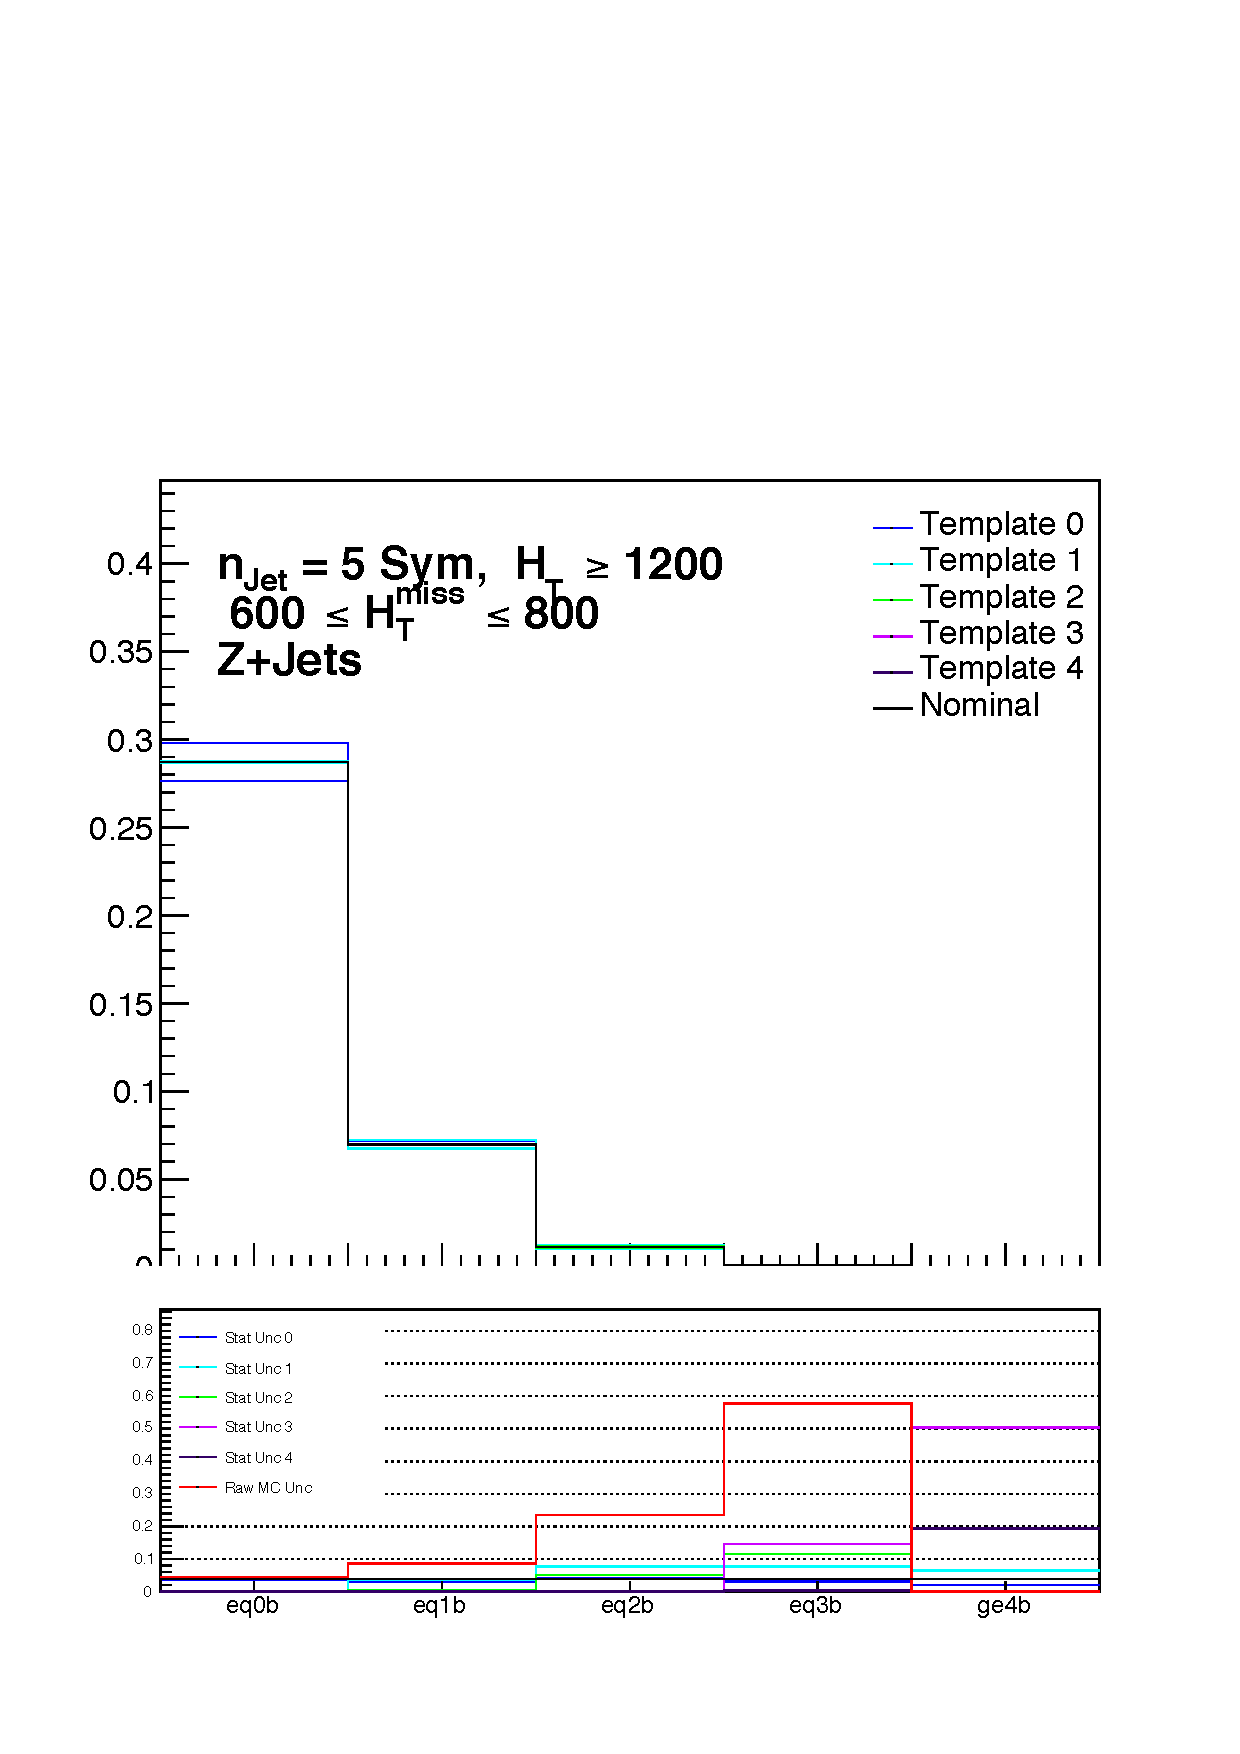
\includegraphics[width=0.45\textwidth]{figures/btagformula/uncertainties/Zinveq5j_1200Inc_600800}
  \caption{\label{fig:formula-uncertainties}
  $n^{\rm tag}$ nominal templates compared to the alternative shapes derived with the toy procedure (``Template0/1/2/3/4'') 
  for the TTJets and WJets processes together (top) and ZToNuNu process (bottom), for some representative (\njet,\scalht,\mht) bins. 
  The bottom pad shows the relative variation with respect to the nominal shape together with the relative statistical uncertainty 
  from the vanilla MC (shown in red).}
\end{figure}

%\section{Characterisation of the signal and control regions}
\label{sec:yields}

A selection of relevant data/MC comparison plots for the signal and
control regions are presented here.  The event selection criteria
defining these regions are detailed in
Sec.~\ref{sec:selection}. Corrections applied to the simulated events
are discussed in Section~\ref{sec:mc-corrections}. The
distributions are shown separately according three \njet categories:
symmetric, asymmetric, and monojet. The distributions are intended to
provide a qualitative understanding of the simulation modelling for
key variables. However, the analysis is not sensitive due to the
reliance on simulation via ratios only (\ie transfer factors) and the
one-to-one mapping of (\njet,~\nb,~\scalht) binning between the
control and signal regions. For monojet, the distributions of
azimuthal angle of jets are included along with other key variables to
demonstrate the absence of beam halo effects. The simulated
distributions are normalized to an integrated luminosity of
36.4~$\ifb$ (the data/MC scale factors are also shown in all plots).

%In addition to distributions, the binned yields in the \mj, \mmj, and
%\gj control samples can be found in
%Tables~\ref{tab:yieldssep_mu_data_sym}-\ref{tab:yieldssep_mu_data_mono},
%\ref{tab:yieldssep_mumu_data_sym}-\ref{tab:yieldssep_mumu_data_mono},
%and \ref{tab:yieldssep_gj_data_sym}-\ref{tab:yieldssep_gj_data_mono},
%respectively, which correspond to an integrated luminosity of 12.9
%\ifb. 
%Breakdown of SM processes for some (\njet,~\nb,~\scalht) bins are shown in Tables
%~\ref{tab:yieldSM-signal} to ~\ref{tab:yieldSM-singlephoton}.
%Finally, Tables~\ref{tab:yieldsnodata_sig_comb_sym},
%\ref{tab:yieldsnodata_sig_comb_asym} and \ref{tab:yieldsnodata_sig_comb_mono} summarise the expected yields, as
%determined from simulation, in the signal region for an integrated
%luminosity of 12.9 \ifb.

%\clearpage
%\subsection{Breakdown of yields from various SM processes}
%\begin{longtable}{| c | c | c | c | c | c | c | c | c  | }
\caption{Summary of yields of each SM process} \label{tab:table} \\    \hline 
$n_{j}$~$n_{b}$~$H_{T}$ & $t\bar{t}$ & $W+jets$ & $Z \rightarrow \nu\nu$ & $DY+jets$ & $Single Top$ & $DiBoson$ & $Multijet$ & Total Yield\\ \hline 
eq2j eq0b 200 & 103.49 & 1026.57 & 1148.86 & 18.24 & 15.98 & 72.15 & 0.00 & 2385.28\\ \hline 
eq2j eq0b 250 & 74.63 & 1050.96 & 1312.16 & 16.09 & 15.33 & 74.25 & 10.11 & 2553.53\\ \hline 
eq2j eq0b 300 & 32.27 & 664.60 & 941.01 & 9.13 & 6.52 & 42.69 & 2.85 & 1699.07\\ \hline 
eq2j eq0b 350 & 12.65 & 395.06 & 569.00 & 5.50 & 1.62 & 17.06 & 1.33 & 1002.24\\ \hline 
eq2j eq0b 400 & 7.22 & 316.98 & 551.29 & 3.96 & 2.22 & 14.28 & 1.51 & 897.46\\ \hline 
eq2j eq0b 500 & 1.33 & 102.97 & 190.11 & 0.79 & 0.01 & 2.12 & 0.00 & 297.31\\ \hline 
eq2j eq0b 600 & 0.47 & 50.93 & 111.12 & 0.29 & 0.54 & 2.69 & 0.00 & 166.04\\ \hline 
eq2j eq0b 800 & 0.52 & 86.65 & 146.22 & 0.39 & 0.00 & 3.16 & 0.00 & 236.94\\ \hline 
eq3j eq1b 200 & 0.57 & 0.00 & 0.32 & 0.00 & 0.00 & 0.00 & 0.00 & 0.89\\ \hline 
eq3j eq1b 250 & 64.13 & 17.16 & 27.10 & 0.54 & 5.36 & 1.22 & 0.00 & 115.51\\ \hline 
eq3j eq1b 300 & 122.13 & 56.55 & 74.29 & 1.00 & 13.99 & 2.69 & 0.00 & 270.64\\ \hline 
eq3j eq1b 350 & 94.34 & 52.60 & 82.06 & 0.85 & 13.66 & 5.30 & 6.22 & 255.03\\ \hline 
eq3j eq1b 400 & 71.61 & 66.57 & 99.75 & 0.82 & 15.02 & 3.06 & 0.43 & 257.26\\ \hline 
eq3j eq1b 500 & 11.23 & 18.94 & 42.91 & 0.24 & 1.88 & 1.61 & 0.00 & 76.82\\ \hline 
eq3j eq1b 600 & 2.92 & 10.44 & 26.73 & 0.12 & 0.66 & 1.20 & 0.00 & 42.06\\ \hline 
eq3j eq1b 800 & 1.93 & 11.73 & 29.27 & 0.07 & 0.54 & 1.37 & 0.00 & 44.92\\ \hline 
eq4j eq2b 200 & 0.00 & 0.00 & 0.00 & 0.00 & 0.00 & 0.00 & 0.00 & 0.00\\ \hline 
eq4j eq2b 250 & 0.20 & 0.00 & 0.02 & 0.00 & 0.00 & 0.00 & 0.00 & 0.22\\ \hline 
eq4j eq2b 300 & 18.30 & 0.75 & 1.98 & 0.01 & 1.38 & 0.00 & 0.00 & 22.42\\ \hline 
eq4j eq2b 350 & 56.98 & 4.03 & 6.78 & 0.08 & 3.56 & 0.00 & 0.00 & 71.43\\ \hline 
eq4j eq2b 400 & 86.02 & 6.97 & 12.42 & 0.11 & 4.54 & 0.60 & 0.00 & 110.66\\ \hline 
eq4j eq2b 500 & 21.45 & 2.68 & 7.27 & 0.05 & 2.76 & 0.25 & 0.00 & 34.46\\ \hline 
eq4j eq2b 600 & 5.24 & 2.02 & 4.38 & 0.02 & 1.26 & 0.05 & 0.00 & 12.98\\ \hline 
eq4j eq2b 800 & 2.66 & 0.00 & 3.79 & 0.02 & 0.58 & 0.00 & 0.00 & 7.06\\ \hline 
ge5j eq0b 200 & 0.00 & 0.00 & 0.00 & 0.00 & 0.00 & 0.00 & 0.00 & 0.00\\ \hline 
ge5j eq0b 250 & 0.00 & 0.00 & 0.00 & 0.00 & 0.00 & 0.00 & 0.00 & 0.00\\ \hline 
ge5j eq0b 300 & 0.03 & 0.00 & 0.05 & 0.00 & 0.00 & 0.00 & 0.00 & 0.07\\ \hline 
ge5j eq0b 350 & 6.96 & 8.88 & 7.98 & 0.26 & 0.00 & 0.39 & 0.02 & 24.49\\ \hline 
ge5j eq0b 400 & 57.77 & 102.86 & 111.49 & 1.65 & 3.35 & 4.48 & 0.00 & 281.60\\ \hline 
ge5j eq0b 500 & 41.04 & 96.56 & 124.97 & 1.30 & 1.62 & 1.67 & 8.83 & 275.99\\ \hline 
ge5j eq0b 600 & 26.59 & 91.74 & 128.08 & 0.96 & 2.62 & 3.95 & 1.72 & 255.67\\ \hline 
ge5j eq0b 800 & 16.75 & 67.00 & 130.94 & 0.76 & 1.84 & 2.45 & 6.82 & 226.57\\ \hline 
    \hline 
    \hline 
\end{longtable}

%\clearpage
%
\begin{longtable}{| c | c | c | c | c | c | c  | }
\caption{Summary of yields of each SM process with green band correction for single mu control region} \label{tab:yieldSM-singlemu} \\    \hline 
$n_{j}$~$n_{b}$~$H_{T}$ & $t\bar{t}$ & $W+jets$ & $DY+jets$ & $Single Top$ & $DiBoson$ & $Multijet$\\ \hline 
eq2j eq0b 200 & 49.72 & 462.03 & 12.22 & 13.20 & 11.00 & 0.00\\ \hline 
eq2j eq0b 250 & 43.63 & 696.98 & 17.99 & 14.91 & 21.91 & 29.43\\ \hline 
eq2j eq0b 300 & 25.93 & 694.87 & 18.48 & 10.09 & 9.60 & 0.00\\ \hline 
eq2j eq0b 350 & 16.12 & 651.65 & 15.93 & 8.28 & 8.68 & 2.06\\ \hline 
eq2j eq0b 400 & 14.27 & 817.43 & 20.20 & 9.19 & 6.81 & 1.48\\ \hline 
eq2j eq0b 500 & 4.54 & 421.47 & 9.11 & 7.35 & 3.41 & 1.78\\ \hline 
eq2j eq0b 600 & 4.53 & 337.94 & 6.84 & 4.88 & 3.14 & 0.04\\ \hline 
eq2j eq0b 800 & 1.75 & 189.75 & 3.45 & 1.01 & 3.54 & 0.87\\ \hline 
eq3j eq1b 200 & 0.75 & 0.36 & 0.00 & 0.19 & 0.00 & 0.00\\ \hline 
eq3j eq1b 250 & 75.46 & 19.58 & 0.43 & 11.84 & 0.32 & 0.00\\ \hline 
eq3j eq1b 300 & 148.89 & 50.89 & 1.86 & 20.80 & 1.66 & 0.00\\ \hline 
eq3j eq1b 350 & 136.62 & 58.21 & 1.97 & 25.78 & 0.72 & 0.00\\ \hline 
eq3j eq1b 400 & 157.15 & 99.79 & 2.90 & 38.57 & 2.24 & 1.40\\ \hline 
eq3j eq1b 500 & 61.56 & 64.65 & 1.97 & 19.55 & 2.95 & 0.17\\ \hline 
eq3j eq1b 600 & 39.88 & 62.71 & 1.62 & 18.90 & 1.38 & 0.18\\ \hline 
eq3j eq1b 800 & 14.32 & 42.72 & 0.96 & 11.82 & 0.51 & 0.45\\ \hline 
eq4j eq2b 200 & 0.00 & 0.00 & 0.00 & 0.00 & 0.00 & 0.00\\ \hline 
eq4j eq2b 250 & 0.58 & 0.00 & 0.00 & 0.04 & 0.00 & 0.00\\ \hline 
eq4j eq2b 300 & 24.25 & 0.40 & 0.05 & 2.44 & 0.00 & 0.00\\ \hline 
eq4j eq2b 350 & 78.01 & 2.84 & 0.06 & 6.14 & 0.00 & 0.00\\ \hline 
eq4j eq2b 400 & 174.10 & 7.82 & 0.28 & 16.06 & 0.22 & 0.69\\ \hline 
eq4j eq2b 500 & 93.31 & 7.37 & 0.27 & 14.76 & 0.33 & 0.00\\ \hline 
eq4j eq2b 600 & 65.49 & 7.41 & 0.29 & 12.46 & 0.05 & 0.00\\ \hline 
eq4j eq2b 800 & 21.14 & 5.52 & 0.16 & 6.98 & 0.00 & 0.00\\ \hline 
ge5j eq0b 200 & 0.00 & 0.00 & 0.00 & 0.00 & 0.00 & 0.00\\ \hline 
ge5j eq0b 250 & 0.00 & 0.00 & 0.00 & 0.00 & 0.00 & 0.00\\ \hline 
ge5j eq0b 300 & 0.07 & 0.19 & 0.01 & 0.00 & 0.33 & 0.00\\ \hline 
ge5j eq0b 350 & 5.10 & 7.62 & 0.30 & 0.21 & 0.10 & 0.00\\ \hline 
ge5j eq0b 400 & 49.27 & 64.97 & 2.42 & 3.05 & 2.14 & 0.64\\ \hline 
ge5j eq0b 500 & 60.81 & 110.72 & 3.07 & 3.99 & 1.55 & 0.18\\ \hline 
ge5j eq0b 600 & 74.42 & 176.44 & 5.00 & 7.23 & 2.47 & 2.68\\ \hline 
ge5j eq0b 800 & 50.81 & 193.80 & 5.31 & 6.95 & 1.96 & 1.28\\ \hline 
    \hline 
    \hline 
\end{longtable}


%\clearpage
%
\begin{longtable}{| c | c | c | c | c | c | c  | }
\caption{Summary of yields of each SM process with green band correction for double mu control region} \label{tab:yieldSM-doublemu} \\    \hline 
$n_{j}$~$n_{b}$~$H_{T}$ & $t\bar{t}$ & $W+jets$ & $DY+jets$ & $Single Top$ & $DiBoson$ & $Multijet$\\ \hline 
eq2j eq0b 200 & 0.30 & 0.00 & 48.76 & 0.00 & 0.72 & 0.00\\ \hline 
eq2j eq0b 250 & 0.76 & 0.00 & 76.51 & 0.21 & 1.43 & 0.00\\ \hline 
eq2j eq0b 300 & 0.24 & 0.00 & 75.50 & 0.04 & 0.94 & 0.00\\ \hline 
eq2j eq0b 350 & 0.37 & 0.00 & 66.59 & 0.17 & 0.70 & 0.00\\ \hline 
eq2j eq0b 400 & 0.19 & 0.00 & 86.99 & 0.21 & 0.69 & 0.00\\ \hline 
eq2j eq0b 500 & 0.15 & 0.00 & 45.77 & 0.00 & 0.36 & 0.00\\ \hline 
eq2j eq0b 600 & 0.04 & 0.00 & 36.53 & 0.00 & 0.18 & 0.00\\ \hline 
eq2j eq0b 800 & 0.02 & 0.00 & 20.22 & 0.00 & 0.20 & 0.00\\ \hline 
eq3j eq1b 200 & 0.00 & 0.00 & 0.00 & 0.00 & 0.00 & 0.00\\ \hline 
eq3j eq1b 250 & 0.91 & 0.00 & 2.58 & 0.00 & 0.00 & 0.00\\ \hline 
eq3j eq1b 300 & 1.34 & 0.00 & 5.41 & 0.11 & 0.00 & 0.00\\ \hline 
eq3j eq1b 350 & 1.15 & 0.00 & 6.85 & 0.61 & 0.24 & 0.00\\ \hline 
eq3j eq1b 400 & 1.75 & 0.00 & 11.28 & 0.10 & 0.18 & 0.00\\ \hline 
eq3j eq1b 500 & 0.83 & 0.00 & 7.53 & 0.16 & 0.31 & 0.00\\ \hline 
eq3j eq1b 600 & 0.99 & 0.00 & 7.21 & 0.11 & 0.23 & 0.00\\ \hline 
eq3j eq1b 800 & 0.61 & 0.00 & 4.83 & 0.00 & 0.30 & 0.00\\ \hline 
eq4j eq2b 200 & 0.00 & 0.00 & 0.00 & 0.00 & 0.00 & 0.00\\ \hline 
eq4j eq2b 250 & 0.00 & 0.00 & 0.00 & 0.00 & 0.00 & 0.00\\ \hline 
eq4j eq2b 300 & 0.13 & 0.00 & 0.21 & 0.00 & 0.00 & 0.00\\ \hline 
eq4j eq2b 350 & 0.75 & 0.00 & 0.42 & 0.00 & 0.07 & 0.00\\ \hline 
eq4j eq2b 400 & 1.24 & 0.00 & 1.24 & 0.02 & 0.00 & 0.00\\ \hline 
eq4j eq2b 500 & 0.80 & 0.00 & 1.02 & 0.14 & 0.00 & 0.00\\ \hline 
eq4j eq2b 600 & 0.58 & 0.00 & 1.05 & 0.14 & 0.00 & 0.00\\ \hline 
eq4j eq2b 800 & 0.60 & 0.00 & 0.74 & 0.12 & 0.00 & 0.00\\ \hline 
ge5j eq0b 200 & 0.00 & 0.00 & 0.00 & 0.00 & 0.00 & 0.00\\ \hline 
ge5j eq0b 250 & 0.00 & 0.00 & 0.00 & 0.00 & 0.00 & 0.00\\ \hline 
ge5j eq0b 300 & 0.00 & 0.00 & 0.00 & 0.00 & 0.00 & 0.00\\ \hline 
ge5j eq0b 350 & 0.00 & 0.00 & 0.58 & 0.00 & 0.00 & 0.00\\ \hline 
ge5j eq0b 400 & 0.20 & 0.00 & 6.73 & 0.08 & 0.00 & 0.00\\ \hline 
ge5j eq0b 500 & 0.14 & 0.00 & 10.68 & 0.00 & 0.24 & 0.00\\ \hline 
ge5j eq0b 600 & 0.75 & 0.00 & 16.98 & 0.00 & 0.28 & 0.00\\ \hline 
ge5j eq0b 800 & 0.42 & 0.00 & 19.90 & 0.00 & 0.27 & 0.00\\ \hline 
    \hline 
    \hline 
\end{longtable}


%\clearpage
%\begin{longtable}{| c | c | c | c  | }
\caption{Summary of yields of each SM process} \label{tab:table} \\    \hline 
$n_{j}$~$n_{b}$~$H_{T}$ & $\gamma+jets$ & $Multijet$ & Total Yield\\ \hline 
eq2j eq0b 200 & 0.00 & 0.00 & 0.00\\ \hline 
eq2j eq0b 250 & 0.00 & 0.00 & 0.00\\ \hline 
eq2j eq0b 300 & 0.00 & 0.00 & 0.00\\ \hline 
eq2j eq0b 350 & 0.00 & 0.00 & 0.00\\ \hline 
eq2j eq0b 400 & 1529.97 & 38.85 & 1568.83\\ \hline 
eq2j eq0b 500 & 596.05 & 7.10 & 603.15\\ \hline 
eq2j eq0b 600 & 344.93 & 6.22 & 351.15\\ \hline 
eq2j eq0b 800 & 940.80 & 10.68 & 951.49\\ \hline 
eq3j eq1b 200 & 0.00 & 0.00 & 0.00\\ \hline 
eq3j eq1b 250 & 0.00 & 0.00 & 0.00\\ \hline 
eq3j eq1b 300 & 0.00 & 0.00 & 0.00\\ \hline 
eq3j eq1b 350 & 0.00 & 0.00 & 0.00\\ \hline 
eq3j eq1b 400 & 257.52 & 2.47 & 259.99\\ \hline 
eq3j eq1b 500 & 137.80 & 4.45 & 142.25\\ \hline 
eq3j eq1b 600 & 100.01 & 3.44 & 103.45\\ \hline 
eq3j eq1b 800 & 196.18 & 10.66 & 206.84\\ \hline 
eq4j eq2b 200 & 0.00 & 0.00 & 0.00\\ \hline 
eq4j eq2b 250 & 0.00 & 0.00 & 0.00\\ \hline 
eq4j eq2b 300 & 0.00 & 0.00 & 0.00\\ \hline 
eq4j eq2b 350 & 0.00 & 0.00 & 0.00\\ \hline 
eq4j eq2b 400 & 22.55 & 0.00 & 22.55\\ \hline 
eq4j eq2b 500 & 20.27 & 0.00 & 20.27\\ \hline 
eq4j eq2b 600 & 18.72 & 1.07 & 19.79\\ \hline 
eq4j eq2b 800 & 22.88 & 1.64 & 24.52\\ \hline 
ge5j eq0b 200 & 0.00 & 0.00 & 0.00\\ \hline 
ge5j eq0b 250 & 0.00 & 0.00 & 0.00\\ \hline 
ge5j eq0b 300 & 0.00 & 0.00 & 0.00\\ \hline 
ge5j eq0b 350 & 0.00 & 0.00 & 0.00\\ \hline 
ge5j eq0b 400 & 257.56 & 0.32 & 257.88\\ \hline 
ge5j eq0b 500 & 363.08 & 6.27 & 369.35\\ \hline 
ge5j eq0b 600 & 452.27 & 12.29 & 464.57\\ \hline 
ge5j eq0b 800 & 847.55 & 216.81 & 1064.36\\ \hline 
    \hline 
    \hline 
\end{longtable}


\newpage
\subsection{Yields and distributions for the muon + jets control sample}

%\begin{table}[h!]
\tiny
\centering
\caption{Yields in the \mj control region for 2.1\ifb for symmetric categories.\label{tab:yieldssep_mu_data_sym}}
\scalebox{0.85}{\begin{tabular}{ccccccccc}
	\hline\hline
	& \multicolumn{8}{c}{\scalht (\gev)} \\ 
	 (\njet,  \nb) & 200-250 & 250-300 & 300-350 & 350-400 & 400-500 & 500-600 & 600-800 & 800-$\infty$ \\ [0.8ex] 
\hline
	(2, 0) & 451 & 660 & 611 & 491 & 615 & 285 & 226 & 116 \\[0.5ex] 
	(2, 1) & 74 & 68 & 57 & 54 & 80 & 49 & 28 & 13 \\[0.5ex] 
	(2, 2) & 2 & 2 & 5 & 1 & 6 & 5 & 2 & -- \\[0.5ex] 
	(3, 0) & 1 & 199 & 419 & 405 & 654 & 356 & 312 & 170 \\[0.5ex] 
	(3, 1) & -- & 86 & 164 & 186 & 235 & 105 & 95 & 31 \\[0.5ex] 
	(3, 2) & -- & 24 & 58 & 57 & 64 & 30 & 18 & 11 \\[0.5ex] 
	(3, $\ge3$) & -- & 1 & -- & -- & 3 & -- & -- & -- \\[0.5ex] 
	(4, 0) & -- & -- & 40 & 142 & 348 & 265 & 265 & 154 \\[0.5ex] 
	(4, 1) & -- & -- & 38 & 130 & 244 & 159 & 130 & 50 \\[0.5ex] 
	(4, 2) & -- & -- & 10 & 54 & 125 & 56 & 55 & 25 \\[0.5ex] 
	(4, $\ge3$) & -- & -- & 1 & 5 & 6 & 4 & 2 & 3 \\[0.5ex] 
	($\ge5$, 0) & -- & -- & -- & 16 & 99 & 132 & 183 & 144 \\[0.5ex] 
	($\ge5$, 1) & -- & -- & -- & 8 & 110 & 159 & 195 & 139 \\[0.5ex] 
	($\ge5$, 2) & -- & -- & -- & 6 & 57 & 90 & 109 & 69 \\[0.5ex] 
	($\ge5$, $\ge3$) & -- & -- & -- & -- & 2 & 6 & 14 & 12 \\[0.5ex] 
	\hline
	\hline
\end{tabular}}
\end{table}

%\begin{table}[h!]
\tiny
\centering
\caption{Data in the \mj control region for 6.26\ifb for asymmetric categories.\label{tab:yieldssep_mu_data_asym}}
\scalebox{0.85}{\begin{tabular}{ccccccccc}
	\hline\hline
	& \multicolumn{8}{c}{\scalht (\gev)} \\ 
	 (\njet,  \nb) & 200-250 & 250-300 & 300-350 & 350-400 & 400-500 & 500-600 & 600-800 & 800-$\infty$ \\ [0.8ex] 
\hline
	(2a, 0) & 12940 & 6805 & 3203 & 1389 & 941 & 242 & 104 & -- \\[0.5ex] 
	(2a, 1) & 2209 & 968 & 431 & 199 & 128 & 29 & -- & -- \\[0.5ex] 
	(2a, 2) & 182 & 84 & 42 & 7 & 8 & -- & -- & -- \\[0.5ex] 
	(3a, 0) & 2846 & 3814 & 2173 & 1104 & 766 & 176 & 60 & -- \\[0.5ex] 
	(3a, 1) & 1524 & 1790 & 912 & 377 & 221 & 37 & 27 & -- \\[0.5ex] 
	(3a, 2) & 419 & 551 & 268 & 96 & 57 & 16 & -- & -- \\[0.5ex] 
	(3a, $\ge3$) & 10 & 24 & 7 & -- & -- & -- & -- & -- \\[0.5ex] 
	(4a, 0) & 26 & 521 & 850 & 544 & 467 & 123 & 39 & -- \\[0.5ex] 
	(4a, 1) & 26 & 457 & 761 & 488 & 332 & 74 & 20 & -- \\[0.5ex] 
	(4a, 2) & 9 & 201 & 382 & 230 & 147 & 29 & 10 & -- \\[0.5ex] 
	(4a, $\ge3$) & -- & 12 & 21 & 23 & 7 & -- & -- & -- \\[0.5ex] 
	($\ge5$a, 0) & -- & 1 & 68 & 171 & 280 & 100 & 30 & -- \\[0.5ex] 
	($\ge5$a, 1) & -- & 3 & 98 & 194 & 306 & 96 & 45 & -- \\[0.5ex] 
	($\ge5$a, 2) & -- & 3 & 46 & 128 & 203 & 66 & 18 & -- \\[0.5ex] 
	($\ge5$a, $\ge3$) & -- & -- & 6 & 15 & 30 & 8 & -- & -- \\[0.5ex] 
	\hline
	\hline
\end{tabular}}
\end{table}

%\begin{table}[h!]
\tiny
\centering
\caption{Yields in the \mj control region for 2.1\ifb for monojet categories.\label{tab:yieldssep_mu_data_mono}}
\begin{tabular}
{ccccccccc}
	\hline\hline
	& \multicolumn{8}{c}{\scalht (\gev)} \\ 
	 (\njet,  \nb) & 200-250 & 250-300 & 300-350 & 350-400 & 400-500 & 500-600 & 600-800 & 800-$\infty$ \\ [0.8ex] 
\hline
	(1, 0) & 4022 & 1498 & 597 & 282 & 246 & 81 & 34 & -- \\[0.5ex] 
	(1, 1) & 196 & 65 & 21 & 14 & 12 & 1 & -- & -- \\[0.5ex] 
	\hline
	\hline
\end{tabular}
\end{table}

%
%\clearpage
\begin{figure}[!h]
    \begin{center}
        \subfigure {\includegraphics[width=0.5\textwidth]{figures/distributions/SingleMu/nJet40_sym_all.pdf}} ~~
        \subfigure {\includegraphics[width=0.5\textwidth]{figures/distributions/SingleMu/ht40_sym_all.pdf}} \\
        \subfigure {\includegraphics[width=0.5\textwidth]{figures/distributions/SingleMu/mht40_pt_sym_all.pdf}} ~~
        \subfigure {\includegraphics[width=0.5\textwidth]{figures/distributions/SingleMu/nBJet40_sym_all.pdf}} \\
        \caption{Key analysis variables for single muon control region (symmetric \njet bins)}
        \label{fig:distribution_singlemu_sym}
    \end{center}
\end{figure}

\clearpage
\begin{figure}[!h]
    \begin{center}
        \subfigure {\includegraphics[width=0.5\textwidth]{figures/distributions/SingleMu/nJet40_asym_all.pdf}} ~~
        \subfigure {\includegraphics[width=0.5\textwidth]{figures/distributions/SingleMu/ht40_asym_all.pdf}} \\
        \subfigure {\includegraphics[width=0.5\textwidth]{figures/distributions/SingleMu/mht40_pt_asym_all.pdf}} ~~
        \subfigure {\includegraphics[width=0.5\textwidth]{figures/distributions/SingleMu/nBJet40_asym_all.pdf}} \\
        \caption{Key analysis variables for single muon control region (asymmetric \njet bins)}
        \label{fig:distribution_singlemu_asym}
    \end{center}
\end{figure}

\clearpage
\begin{figure}[!h]
    \begin{center}        
        \subfigure {\includegraphics[width=0.5\textwidth]{figures/distributions/SingleMu/jet_pt[0]_mono_all.pdf}} ~~
        \subfigure {\includegraphics[width=0.5\textwidth]{figures/distributions/SingleMu/njetInc_mono_all.pdf}} \\
        \subfigure {\includegraphics[width=0.5\textwidth]{figures/distributions/SingleMu/nBJet40_mono_all.pdf}} ~~
        \subfigure {\includegraphics[width=0.5\textwidth]{figures/distributions/SingleMu/jet_phi[0]_mono_all.pdf}} \\
        \caption{Key analysis variables for single muon control region (monojet bins)}
        \label{fig:distribution_singlemu_mono}
    \end{center}
\end{figure}

\newpage
\subsection{Yields and distributions for the di-muon + jets control sample}

%\begin{table}[h!]
\tiny
\centering
\topcaption{Yields in the \mmj control region for 1.26\ifb for symmetric categories. The letter ``a'' in jet \eg ``2a''  indicates the asymmetric jet bins. All entries are non-zero but are truncated to one decimal place.\label{tab:yieldssep_data_mumu_sym}}
\begin{tabular}
{ccccccccc}
	\hline\hline
&	& \multicolumn{8}{c}{\scalht (\gev)} \\ 
	 (\njet,  \nb) & 200-250 & 250-300 & 300-350 & 350-400 & 400-500 & 500-600 & 600-800 & 800-$\infty$ \\ [0.8ex] 
\hline
	(2, 0) & 37 & 45 & 41 & 23 & 33 & 25 & 12 & 6 \\[0.5ex] 
	(2, 1) & 3 & 5 & 8 & 2 & 5 & 1 & 1 & 1 \\[0.5ex] 
	(2, 2) & 0 & 0 & 0 & -- & 0 & 0 & 0 & 0 \\[0.5ex] 
	(3, 0) & 0 & 8 & 25 & 27 & 30 & 23 & 10 & 10 \\[0.5ex] 
	(3, 1) & 0 & 2 & 3 & 4 & 1 & 1 & 4 & 2 \\[0.5ex] 
	(3, 2) & -- & 1 & 2 & 0 & 0 & 0 & 1 & 0 \\[0.5ex] 
	(3, $\ge3$) & -- & -- & -- & 0 & 0 & 0 & -- & -- \\[0.5ex] 
	(4, 0) & -- & -- & 3 & 1 & 13 & 11 & 16 & 10 \\[0.5ex] 
	(4, 1) & -- & -- & 1 & 1 & 2 & 0 & 3 & 4 \\[0.5ex] 
	(4, 2) & -- & -- & 0 & 0 & 0 & 0 & 0 & 1 \\[0.5ex] 
	(4, $\ge3$) & -- & -- & -- & 0 & 0 & 0 & 0 & 0 \\[0.5ex] 
	($\ge5$, 0) & -- & -- & -- & 0 & 2 & 4 & 5 & 10 \\[0.5ex] 
	($\ge5$, 1) & -- & -- & -- & 0 & 1 & 4 & 2 & 2 \\[0.5ex] 
	($\ge5$, 2) & -- & -- & -- & 0 & 0 & 0 & 1 & 2 \\[0.5ex] 
	($\ge5$, $\ge3$) & -- & -- & -- & -- & 1 & 0 & 0 & 0 \\[0.5ex] 
	\hline
	\hline
\end{tabular}
\end{table}

%\begin{table}[h!]
\tiny
\centering
\caption{Data in the \mmj control region for 12.9\ifb for asymmetric categories.\label{tab:yieldssep_mumu_data_asym}}
\scalebox{0.85}{\begin{tabular}{ccccccccc}
	\hline\hline
	& \multicolumn{8}{c}{\scalht (\gev)} \\ 
	 (\njet,  \nb) & 200-250 & 250-300 & 300-350 & 350-400 & 400-500 & 500-600 & 600-800 & 800-$\infty$ \\ [0.8ex] 
\hline
	(2a, 0) & 2405 & 1362 & 691 & 295 & 239 & 60 & 20 & -- \\[0.5ex] 
	(2a, 1) & 289 & 144 & 78 & 31 & 20 & 7 & -- & -- \\[0.5ex] 
	(2a, 2) & 36 & 19 & 11 & 3 & 0 & -- & -- & -- \\[0.5ex] 
	(3a, 0) & 434 & 600 & 352 & 199 & 157 & 39 & 11 & -- \\[0.5ex] 
	(3a, 1) & 67 & 98 & 78 & 24 & 28 & 14 & 0 & -- \\[0.5ex] 
	(3a, 2) & 15 & 14 & 15 & 10 & 4 & 0 & -- & -- \\[0.5ex] 
	(3a, $\ge3$) & 0 & 0 & 0 & -- & -- & -- & -- & -- \\[0.5ex] 
	(4a, 0) & 2 & 57 & 105 & 69 & 67 & 14 & 3 & -- \\[0.5ex] 
	(4a, 1) & 2 & 16 & 31 & 21 & 16 & 3 & 1 & -- \\[0.5ex] 
	(4a, 2) & 0 & 5 & 15 & 4 & 3 & 0 & 0 & -- \\[0.5ex] 
	(4a, $\ge3$) & -- & 0 & 1 & 0 & 1 & -- & -- & -- \\[0.5ex] 
	($\ge5$a, 0) & -- & 0 & 6 & 17 & 26 & 14 & 6 & -- \\[0.5ex] 
	($\ge5$a, 1) & -- & 0 & 3 & 3 & 15 & 3 & 0 & -- \\[0.5ex] 
	($\ge5$a, 2) & -- & 1 & 1 & 4 & 2 & 1 & 0 & -- \\[0.5ex] 
	($\ge5$a, $\ge3$) & -- & -- & 0 & 1 & 1 & 0 & -- & -- \\[0.5ex] 
	\hline
	\hline
\end{tabular}}
\end{table}

%\begin{table}[h!]
\tiny
\centering
\caption{Data in the \mmj control region for 2.2\ifb for monojet categories.\label{tab:yieldssep_mumu_data_mono}}
\scalebox{0.85}{\begin{tabular}{ccccccccc}
	\hline\hline
	& \multicolumn{8}{c}{\scalht (\gev)} \\ 
	 (\njet,  \nb) & 200-250 & 250-300 & 300-350 & 350-400 & 400-500 & 500-600 & 600-800 & 800-$\infty$ \\ [0.8ex] 
\hline
	(1, 0) & 518 & 193 & 99 & 37 & 31 & 14 & 6 & -- \\[0.5ex] 
	(1, 1) & 18 & 13 & 6 & 0 & 1 & 1 & -- & -- \\[0.5ex] 
	\hline
	\hline
\end{tabular}}
\end{table}

%
%\clearpage
\begin{figure}[!h]
    \begin{center}
        \subfigure {\includegraphics[width=0.5\textwidth]{figures/distributions/DoubleMu/nJet40_sym_all.pdf}} ~~
        \subfigure {\includegraphics[width=0.5\textwidth]{figures/distributions/DoubleMu/ht40_sym_all.pdf}} \\
        \subfigure {\includegraphics[width=0.5\textwidth]{figures/distributions/DoubleMu/mht40_pt_sym_all.pdf}} ~~
        \subfigure {\includegraphics[width=0.5\textwidth]{figures/distributions/DoubleMu/nBJet40_sym_all.pdf}} \\
        \caption{Key analysis variables for double muon control region (symmetric \njet bins)}
        \label{fig:distribution_doublemu_sym}
    \end{center}
\end{figure}

\clearpage
\begin{figure}[!h]
    \begin{center}
        \subfigure {\includegraphics[width=0.5\textwidth]{figures/distributions/DoubleMu/nJet40_asym_all.pdf}} ~~
        \subfigure {\includegraphics[width=0.5\textwidth]{figures/distributions/DoubleMu/ht40_asym_all.pdf}} \\
        \subfigure {\includegraphics[width=0.5\textwidth]{figures/distributions/DoubleMu/mht40_pt_asym_all.pdf}} ~~
        \subfigure {\includegraphics[width=0.5\textwidth]{figures/distributions/DoubleMu/nBJet40_asym_all.pdf}} \\
        \caption{Key analysis variables for double muon control region (asymmetric \njet bins)}
        \label{fig:distribution_doublemu_asym}
    \end{center}
\end{figure}

\clearpage
\begin{figure}[!h]
    \begin{center} 
        \subfigure {\includegraphics[width=0.5\textwidth]{figures/distributions/DoubleMu/jet_pt[0]_mono_all.pdf}} ~~
        \subfigure {\includegraphics[width=0.5\textwidth]{figures/distributions/DoubleMu/njetInc_mono_all.pdf}} \\
        \subfigure {\includegraphics[width=0.5\textwidth]{figures/distributions/DoubleMu/nBJet40_mono_all.pdf}} ~~
        \subfigure {\includegraphics[width=0.5\textwidth]{figures/distributions/DoubleMu/jet_phi[0]_mono_all.pdf}} \\
        \caption{Key analysis variables for double muon control region (monojet bins)}
        \label{fig:distribution_doublemu_mono}
    \end{center}
\end{figure}

\newpage
\subsection{Yields and distributions for the photon + jets control sample}

%\begin{table}[h!]
\tiny
\centering
\caption{Yields in the \gj control region for 1.26\ifb for symmetric categories. The letter ``a'' in jet \eg ``2a''  indicates the asymmetric jet bins. All entries are non-zero but are truncated to one decimal place.\label{tab:yieldssep_data_gj_sym}}
\begin{tabular}
{ccccc}
	\hline\hline
&	& \multicolumn{4}{c}{\scalht (\gev)} \\ 
	 (\njet,  \nb) & 400-500 & 500-600 & 600-800 & 800-$\infty$ \\ [0.8ex] 
\hline
	(2, 0) & 189 & 65 & 37 & 76 \\[0.5ex] 
	(2, 1) & 9 & 1 & 0 & 7 \\[0.5ex] 
	(2, 2) & 0 & 0 & 0 & 0 \\[0.5ex] 
	(3, 0) & 272 & 122 & 69 & 132 \\[0.5ex] 
	(3, 1) & 23 & 13 & 8 & 24 \\[0.5ex] 
	(3, 2) & 4 & 0 & 2 & 1 \\[0.5ex] 
	(3, $\ge3$) & 1 & 0 & -- & -- \\[0.5ex] 
	(4, 0) & 132 & 92 & 73 & 83 \\[0.5ex] 
	(4, 1) & 20 & 16 & 6 & 22 \\[0.5ex] 
	(4, 2) & 2 & 1 & 1 & 2 \\[0.5ex] 
	(4, $\ge3$) & 0 & 0 & 1 & 0 \\[0.5ex] 
	($\ge5$, 0) & 26 & 40 & 49 & 63 \\[0.5ex] 
	($\ge5$, 1) & 3 & 5 & 9 & 15 \\[0.5ex] 
	($\ge5$, 2) & 2 & 3 & 1 & 4 \\[0.5ex] 
	($\ge5$, $\ge3$) & 0 & 0 & 0 & 0 \\[0.5ex] 
	\hline
	\hline
\end{tabular}
\end{table}

%\begin{table}[h!]
\tiny
\centering
\caption{Data in the \gj control region for 2.2\ifb for asymmetric categories.\label{tab:yieldssep_gj_data_asym}}
\scalebox{0.85}{\begin{tabular}{ccccc}
	\hline\hline
	& \multicolumn{4}{c}{\scalht (\gev)} \\ 
	 (\njet,  \nb) & 400-500 & 500-600 & 600-800 & 800-$\infty$ \\ [0.8ex] 
\hline
	(2a, 0) & 164 & 44 & 17 & -- \\[0.5ex] 
	(2a, 1) & 16 & 2 & -- & -- \\[0.5ex] 
	(2a, 2) & 1 & -- & -- & -- \\[0.5ex] 
	(3a, 0) & 105 & 17 & 8 & -- \\[0.5ex] 
	(3a, 1) & 7 & 2 & 2 & -- \\[0.5ex] 
	(3a, 2) & 1 & 0 & -- & -- \\[0.5ex] 
	(3a, $\ge3$) & -- & -- & -- & -- \\[0.5ex] 
	(4a, 0) & 112 & 13 & 3 & -- \\[0.5ex] 
	(4a, 1) & 16 & 5 & 0 & -- \\[0.5ex] 
	(4a, 2) & 1 & 0 & 0 & -- \\[0.5ex] 
	(4a, $\ge3$) & 0 & -- & -- & -- \\[0.5ex] 
	($\ge5$a, 0) & 55 & 12 & 4 & -- \\[0.5ex] 
	($\ge5$a, 1) & 10 & 6 & 0 & -- \\[0.5ex] 
	($\ge5$a, 2) & 3 & 0 & 0 & -- \\[0.5ex] 
	($\ge5$a, $\ge3$) & 0 & 0 & -- & -- \\[0.5ex] 
	\hline
	\hline
\end{tabular}}
\end{table}

%\begin{table}[h!]
\tiny
\centering
\caption{Data in the \gj control region for 2.1\ifb for monojet categories.\label{tab:yieldssep_gj_data_mono}}
\scalebox{0.85}{\begin{tabular}{ccccc}
	\hline\hline
	& \multicolumn{4}{c}{\scalht (\gev)} \\ 
	 (\njet,  \nb) & 400-500 & 500-600 & 600-800 & 800-$\infty$ \\ [0.8ex] 
\hline
	(1, 0) & 565 & 181 & 69 & -- \\[0.5ex] 
	(1, 1) & 23 & 6 & -- & -- \\[0.5ex] 
	\hline
	\hline
\end{tabular}}
\end{table}

%
%\clearpage
\begin{figure}[!h]
    \begin{center}
        \subfigure {\includegraphics[width=0.5\textwidth]{figures/distributions/SinglePhoton/nJet40_sym_all.pdf}} ~~
        \subfigure {\includegraphics[width=0.5\textwidth]{figures/distributions/SinglePhoton/ht40_sym_all.pdf}} \\
        \subfigure {\includegraphics[width=0.5\textwidth]{figures/distributions/SinglePhoton/mht40_pt_sym_all.pdf}} ~~
        \subfigure {\includegraphics[width=0.5\textwidth]{figures/distributions/SinglePhoton/nBJet40_sym_all.pdf}} \\
        \caption{Key analysis variables for single photon control region (symmetric \njet bins)}
        \label{fig:distribution_singlephoton_sym}
    \end{center}
\end{figure}

\clearpage
\begin{figure}[!h]
    \begin{center}
        \subfigure {\includegraphics[width=0.5\textwidth]{figures/distributions/SinglePhoton/nJet40_asym_all.pdf}} ~~
        \subfigure {\includegraphics[width=0.5\textwidth]{figures/distributions/SinglePhoton/ht40_asym_all.pdf}} \\
        \subfigure {\includegraphics[width=0.5\textwidth]{figures/distributions/SinglePhoton/mht40_pt_asym_all.pdf}} ~~
        \subfigure {\includegraphics[width=0.5\textwidth]{figures/distributions/SinglePhoton/nBJet40_asym_all.pdf}} \\
        \caption{Key analysis variables for single photon control region (asymmetric \njet bins)}
        \label{fig:distribution_singlephoton_asym}
    \end{center}
\end{figure}

\clearpage
\begin{figure}[!h]
    \begin{center} 
        \subfigure {\includegraphics[width=0.5\textwidth]{figures/distributions/SinglePhoton/jet_pt[0]_mono_all.pdf}} ~~
        \subfigure {\includegraphics[width=0.5\textwidth]{figures/distributions/SinglePhoton/njetInc_mono_all.pdf}} \\
        \subfigure {\includegraphics[width=0.5\textwidth]{figures/distributions/SinglePhoton/nBJet40_mono_all.pdf}} ~~
        \subfigure {\includegraphics[width=0.5\textwidth]{figures/distributions/SinglePhoton/jet_phi[0]_mono_all.pdf}} \\
        \caption{Key analysis variables for single photon control region (monojet bins)}
        \label{fig:distribution_singlephoton_mono}
    \end{center}
\end{figure}

\newpage
\subsection{Expected yields and distributions in the signal region}

%In the absence of multijet events from QCD, the remaining significant
%backgrounds in the signal region are expected to stem from SM
%processes with genuine \met in the final state. For the low jet
%multiplicity categories, the largest backgrounds with genuine \met are
%from the associated production of W or Z bosons with jets, followed by
%either the weak decays \znunu\ or \wtaunu, where the $\tau$ decays
%hadronically and is identified as a jet, or by leptonic decays that
%are outside acceptance or not rejected by the dedicated electron or
%muon vetoes. For the higher jet multiplicity categories, top quark
%production followed by semileptonic weak top quark decay becomes
%dominant. The relative contribution from \ttbar depends on the jet
%multiplicity with increase importance for large jet multiplicities.

%Tables~\ref{tab:yieldsnodata_sig_comb_sym},
%\ref{tab:yieldsnodata_sig_comb_asym} and \ref{tab:yieldsnodata_sig_comb_mono} 
%summarise the expected yields, as
%determined from simulation, in the signal region for an integrated
%luminosity of 12.9 \ifb. In addition to the total expected yield (SM)
%per (\njet,~\nb,~\scalht) bin, the $\ttbar$W and \znunu\ contributions
%are also shown (the former of which contains all residual
%contributions from sub-dominant processes such as \eg diboson
%production). These numbers are indicative only.
%
%\clearpage
%\begin{table}[h!]
\tiny
\centering
\caption{Yields in the signal region for 2.24\ifb for symmetric categories. All entries are non-zero but are truncated to one decimal place.\label{tab:yieldsnodata_sig_comb_sym}}
\scalebox{0.85}{\begin{tabular}{cccccccccc}
	\hline\hline
	&	& \multicolumn{8}{c}{\scalht (\gev)}\\ 
	&	 (\njet, \nb) & 200-250 & 250-300 & 300-350 & 350-400 & 400-500 & 500-600 & 600-800 & 800-$\infty$ \\ [0.8ex] 
\hline
	SM & (2, 0) & $1022.3\pm 57.7$ & $1054.7\pm 31.0$ & $717.2\pm 26.3$ & $437.4\pm 25.5$ & $389.5\pm 16.3$ & $130.7\pm 4.2$ & $60.2\pm 1.6$ & $73.4\pm 1.6$ \\[0.5ex] 
	Ttw & (2, 0) & $478.0\pm 15.4$ & $473.5\pm 15.2$ & $308.1\pm 11.6$ & $166.3\pm 7.7$ & $140.3\pm 5.6$ & $44.1\pm 2.7$ & $18.4\pm 1.0$ & $23.1\pm 1.1$ \\[0.5ex] 
	Zinv & (2, 0) & $495.6\pm 8.3$ & $556.6\pm 7.9$ & $388.0\pm 6.5$ & $248.7\pm 5.0$ & $235.1\pm 4.3$ & $84.9\pm 2.4$ & $41.9\pm 1.2$ & $50.3\pm 1.1$ \\[0.5ex] 
	SM & (2, 1) & $97.7\pm 6.8$ & $88.2\pm 4.5$ & $59.1\pm 3.8$ & $36.0\pm 3.1$ & $31.3\pm 2.2$ & $11.0\pm 1.0$ & $6.1\pm 0.4$ & $7.4\pm 0.4$ \\[0.5ex] 
	Ttw & (2, 1) & $59.8\pm 3.8$ & $46.2\pm 3.4$ & $27.3\pm 2.7$ & $13.1\pm 2.0$ & $10.5\pm 1.3$ & $3.7\pm 0.8$ & $1.6\pm 0.2$ & $2.2\pm 0.2$ \\[0.5ex] 
	Zinv & (2, 1) & $33.2\pm 2.1$ & $39.9\pm 2.1$ & $30.1\pm 1.8$ & $21.1\pm 1.4$ & $19.7\pm 1.2$ & $7.2\pm 0.7$ & $4.5\pm 0.4$ & $5.2\pm 0.4$ \\[0.5ex] 
	SM & (2, 2) & $6.1\pm 0.9$ & $7.0\pm 1.0$ & $5.0\pm 0.9$ & $2.3\pm 0.5$ & $2.0\pm 0.4$ & $1.1\pm 0.4$ & $0.3\pm 0.1$ & -- \\[0.5ex] 
	Ttw & (2, 2) & $2.9\pm 0.6$ & $2.9\pm 0.8$ & $2.8\pm 0.8$ & $0.9\pm 0.4$ & $0.7\pm 0.3$ & $0.7\pm 0.3$ & $0.0\pm 0.0$ & -- \\[0.5ex] 
	Zinv & (2, 2) & $2.9\pm 0.6$ & $3.9\pm 0.6$ & $2.1\pm 0.5$ & $1.2\pm 0.3$ & $1.2\pm 0.3$ & $0.4\pm 0.1$ & $0.2\pm 0.1$ & -- \\[0.5ex] 
	SM & (3, 0) & $2.1\pm 0.7$ & $190.1\pm 8.7$ & $547.9\pm 33.6$ & $561.0\pm 46.8$ & $628.9\pm 26.4$ & $233.1\pm 9.4$ & $123.7\pm 2.4$ & $103.8\pm 1.7$ \\[0.5ex] 
	Ttw & (3, 0) & $1.2\pm 0.7$ & $88.7\pm 5.9$ & $261.6\pm 10.4$ & $249.9\pm 9.2$ & $264.1\pm 7.6$ & $88.2\pm 3.7$ & $40.9\pm 1.6$ & $32.4\pm 1.0$ \\[0.5ex] 
	Zinv & (3, 0) & $0.8\pm 0.3$ & $96.6\pm 3.3$ & $256.5\pm 5.3$ & $266.9\pm 5.1$ & $340.8\pm 5.3$ & $137.8\pm 3.0$ & $82.8\pm 1.7$ & $71.4\pm 1.4$ \\[0.5ex] 
	SM & (3, 1) & -- & $41.0\pm 2.8$ & $95.7\pm 6.7$ & $99.7\pm 8.9$ & $103.6\pm 5.4$ & $34.1\pm 2.2$ & $17.4\pm 0.9$ & $14.8\pm 0.7$ \\[0.5ex] 
	Ttw & (3, 1) & -- & $30.2\pm 2.3$ & $64.6\pm 3.4$ & $60.8\pm 3.4$ & $58.1\pm 3.0$ & $16.8\pm 1.6$ & $6.8\pm 0.7$ & $4.9\pm 0.5$ \\[0.5ex] 
	Zinv & (3, 1) & -- & $9.7\pm 1.0$ & $25.9\pm 1.6$ & $31.0\pm 1.7$ & $41.6\pm 1.8$ & $16.2\pm 1.0$ & $10.7\pm 0.6$ & $9.9\pm 0.5$ \\[0.5ex] 
	SM & (3, 2) & -- & $5.4\pm 0.7$ & $17.0\pm 1.6$ & $19.5\pm 2.3$ & $15.2\pm 1.2$ & $4.4\pm 0.6$ & $1.4\pm 0.2$ & $1.1\pm 0.2$ \\[0.5ex] 
	Ttw & (3, 2) & -- & $3.9\pm 0.6$ & $12.9\pm 1.2$ & $14.8\pm 1.6$ & $10.5\pm 0.9$ & $2.6\pm 0.4$ & $0.4\pm 0.1$ & $0.4\pm 0.1$ \\[0.5ex] 
	Zinv & (3, 2) & -- & $1.4\pm 0.4$ & $3.1\pm 0.5$ & $3.2\pm 0.5$ & $4.1\pm 0.6$ & $1.7\pm 0.4$ & $1.0\pm 0.2$ & $0.7\pm 0.1$ \\[0.5ex] 
	SM & (3, $\ge3$) & -- & $0.1\pm 0.1$ & -- & -- & $0.3\pm 0.1$ & -- & -- & -- \\[0.5ex] 
	Ttw & (3, $\ge3$) & -- & $0.1\pm 0.1$ & -- & -- & $0.2\pm 0.1$ & -- & -- & -- \\[0.5ex] 
	Zinv & (3, $\ge3$) & -- & $0.0\pm 0.0$ & -- & -- & $0.1\pm 0.1$ & -- & -- & -- \\[0.5ex] 
	SM & (4, 0) & -- & -- & $82.3\pm 5.4$ & $226.3\pm 9.3$ & $426.1\pm 8.4$ & $203.1\pm 4.7$ & $128.3\pm 2.5$ & $90.3\pm 1.6$ \\[0.5ex] 
	Ttw & (4, 0) & -- & -- & $45.5\pm 4.2$ & $121.0\pm 6.3$ & $216.7\pm 7.0$ & $84.6\pm 3.7$ & $48.0\pm 1.8$ & $31.5\pm 1.0$ \\[0.5ex] 
	Zinv & (4, 0) & -- & -- & $34.6\pm 2.0$ & $100.0\pm 3.1$ & $207.6\pm 4.2$ & $118.3\pm 2.9$ & $80.4\pm 1.7$ & $58.8\pm 1.2$ \\[0.5ex] 
	SM & (4, 1) & -- & -- & $26.5\pm 2.1$ & $76.3\pm 3.7$ & $114.3\pm 3.5$ & $47.3\pm 2.2$ & $25.9\pm 1.2$ & $18.3\pm 0.9$ \\[0.5ex] 
	Ttw & (4, 1) & -- & -- & $21.7\pm 1.8$ & $60.1\pm 2.9$ & $84.5\pm 3.1$ & $29.4\pm 1.9$ & $13.3\pm 1.0$ & $7.2\pm 0.7$ \\[0.5ex] 
	Zinv & (4, 1) & -- & -- & $4.1\pm 0.6$ & $14.4\pm 1.2$ & $29.4\pm 1.5$ & $17.9\pm 1.1$ & $12.6\pm 0.7$ & $11.0\pm 0.5$ \\[0.5ex] 
	SM & (4, 2) & -- & -- & $8.0\pm 0.8$ & $22.3\pm 1.5$ & $37.2\pm 1.8$ & $11.3\pm 0.9$ & $4.1\pm 0.5$ & $3.1\pm 0.4$ \\[0.5ex] 
	Ttw & (4, 2) & -- & -- & $6.6\pm 0.7$ & $20.2\pm 1.3$ & $32.0\pm 1.7$ & $9.1\pm 0.8$ & $2.5\pm 0.5$ & $1.5\pm 0.3$ \\[0.5ex] 
	Zinv & (4, 2) & -- & -- & $1.1\pm 0.3$ & $1.5\pm 0.4$ & $5.1\pm 0.6$ & $2.2\pm 0.4$ & $1.6\pm 0.2$ & $1.6\pm 0.2$ \\[0.5ex] 
	SM & (4, $\ge3$) & -- & -- & $0.4\pm 0.2$ & $1.7\pm 0.4$ & $3.2\pm 0.5$ & $0.8\pm 0.3$ & $0.1\pm 0.1$ & $0.1\pm 0.0$ \\[0.5ex] 
	Ttw & (4, $\ge3$) & -- & -- & $0.4\pm 0.2$ & $1.4\pm 0.3$ & $2.9\pm 0.4$ & $0.6\pm 0.3$ & $0.1\pm 0.0$ & $0.1\pm 0.0$ \\[0.5ex] 
	Zinv & (4, $\ge3$) & -- & -- & $0.0\pm 0.0$ & $0.3\pm 0.2$ & $0.3\pm 0.2$ & $0.2\pm 0.1$ & $0.1\pm 0.0$ & $0.0\pm 0.0$ \\[0.5ex] 
	SM & ($\ge5$, 0) & -- & -- & -- & $12.0\pm 2.8$ & $125.2\pm 8.1$ & $115.5\pm 10.4$ & $105.6\pm 2.9$ & $82.6\pm 1.6$ \\[0.5ex] 
	Ttw & ($\ge5$, 0) & -- & -- & -- & $7.8\pm 1.6$ & $74.1\pm 4.1$ & $54.9\pm 2.9$ & $49.1\pm 2.3$ & $32.9\pm 1.0$ \\[0.5ex] 
	Zinv & ($\ge5$, 0) & -- & -- & -- & $4.2\pm 0.6$ & $45.2\pm 2.0$ & $51.5\pm 1.9$ & $56.0\pm 1.6$ & $49.7\pm 1.2$ \\[0.5ex] 
	SM & ($\ge5$, 1) & -- & -- & -- & $5.7\pm 1.3$ & $65.7\pm 4.3$ & $55.6\pm 5.2$ & $38.9\pm 1.7$ & $27.4\pm 1.0$ \\[0.5ex] 
	Ttw & ($\ge5$, 1) & -- & -- & -- & $5.0\pm 0.7$ & $54.4\pm 2.4$ & $41.6\pm 2.0$ & $27.7\pm 1.5$ & $16.6\pm 0.8$ \\[0.5ex] 
	Zinv & ($\ge5$, 1) & -- & -- & -- & $0.7\pm 0.2$ & $8.3\pm 0.8$ & $9.7\pm 0.8$ & $11.0\pm 0.7$ & $10.9\pm 0.6$ \\[0.5ex] 
	SM & ($\ge5$, 2) & -- & -- & -- & $2.3\pm 0.6$ & $27.0\pm 2.0$ & $22.4\pm 2.2$ & $11.9\pm 0.9$ & $8.3\pm 0.6$ \\[0.5ex] 
	Ttw & ($\ge5$, 2) & -- & -- & -- & $2.1\pm 0.4$ & $24.4\pm 1.3$ & $18.4\pm 1.2$ & $9.8\pm 0.9$ & $6.3\pm 0.6$ \\[0.5ex] 
	Zinv & ($\ge5$, 2) & -- & -- & -- & $0.2\pm 0.1$ & $1.4\pm 0.3$ & $2.2\pm 0.4$ & $2.1\pm 0.3$ & $2.0\pm 0.2$ \\[0.5ex] 
	SM & ($\ge5$, $\ge3$) & -- & -- & -- & -- & $3.0\pm 0.5$ & $3.3\pm 0.5$ & $2.0\pm 0.4$ & $1.2\pm 0.2$ \\[0.5ex] 
	Ttw & ($\ge5$, $\ge3$) & -- & -- & -- & -- & $2.7\pm 0.4$ & $2.9\pm 0.5$ & $1.6\pm 0.4$ & $0.9\pm 0.2$ \\[0.5ex] 
	Zinv & ($\ge5$, $\ge3$) & -- & -- & -- & -- & $0.1\pm 0.1$ & $0.2\pm 0.1$ & $0.5\pm 0.2$ & $0.3\pm 0.1$ \\[0.5ex] 
	\hline
	\hline
\end{tabular}}
\end{table}

%\clearpage
%\begin{table}[h!]
\tiny
\centering
\caption{Yields in the signal region for 6.26\ifb for asymmetric categories. The letter ``a'' in jet \eg ``2a''  indicates the asymmetric jet bins. All entries are non-zero but are truncated to one decimal place.\label{tab:yieldsnodata_sig_comb_asym}}
\scalebox{0.85}{\begin{tabular}{cccccccccc}
	\hline\hline
	&	& \multicolumn{8}{c}{\scalht (\gev)}\\ 
	&	 (\njet, \nb) & 200-250 & 250-300 & 300-350 & 350-400 & 400-500 & 500-600 & 600-800 & 800-$\infty$ \\ [0.8ex] 
\hline
	SM & (2a, 0) & $12214.0\pm 233.4$ & $3665.5\pm 46.8$ & $1354.8\pm 16.2$ & $537.2\pm 10.1$ & $360.9\pm 9.4$ & $79.5\pm 6.3$ & $42.1\pm 10.9$ & -- \\[0.5ex] 
	Ttw & (2a, 0) & $5992.0\pm 47.7$ & $1653.1\pm 25.0$ & $567.0\pm 14.8$ & $205.2\pm 8.6$ & $119.5\pm 6.2$ & $18.6\pm 2.8$ & $11.1\pm 4.2$ & -- \\[0.5ex] 
	Zinv & (2a, 0) & $6001.6\pm 17.7$ & $1975.6\pm 8.9$ & $787.8\pm 6.0$ & $332.0\pm 4.8$ & $241.4\pm 4.9$ & $60.9\pm 2.2$ & $28.6\pm 0.7$ & -- \\[0.5ex] 
	SM & (2a, 1) & $1296.9\pm 27.9$ & $345.6\pm 8.0$ & $113.9\pm 3.9$ & $49.2\pm 2.7$ & $31.8\pm 2.2$ & $7.4\pm 1.1$ & -- & -- \\[0.5ex] 
	Ttw & (2a, 1) & $786.2\pm 13.1$ & $185.3\pm 6.7$ & $51.9\pm 3.5$ & $20.5\pm 2.3$ & $10.7\pm 1.6$ & $2.6\pm 0.9$ & -- & -- \\[0.5ex] 
	Zinv & (2a, 1) & $487.3\pm 4.7$ & $156.8\pm 2.4$ & $62.0\pm 1.6$ & $28.7\pm 1.4$ & $21.1\pm 1.4$ & $4.7\pm 0.6$ & -- & -- \\[0.5ex] 
	SM & (2a, 2) & $91.5\pm 3.8$ & $22.8\pm 1.7$ & $6.6\pm 0.9$ & $2.2\pm 0.5$ & $2.3\pm 0.6$ & -- & -- & -- \\[0.5ex] 
	Ttw & (2a, 2) & $53.8\pm 3.2$ & $13.1\pm 1.6$ & $3.1\pm 0.8$ & $0.9\pm 0.4$ & $1.1\pm 0.5$ & -- & -- & -- \\[0.5ex] 
	Zinv & (2a, 2) & $36.1\pm 1.2$ & $9.5\pm 0.5$ & $3.6\pm 0.4$ & $1.3\pm 0.3$ & $1.2\pm 0.3$ & -- & -- & -- \\[0.5ex] 
	SM & (3a, 0) & $3265.1\pm 73.5$ & $3282.9\pm 62.0$ & $1719.2\pm 77.8$ & $577.5\pm 27.9$ & $257.5\pm 7.2$ & $42.1\pm 4.8$ & $20.7\pm 504.6$ & -- \\[0.5ex] 
	Ttw & (3a, 0) & $1788.2\pm 24.4$ & $1731.6\pm 24.1$ & $839.0\pm 17.2$ & $251.4\pm 9.4$ & $106.9\pm 6.0$ & $12.3\pm 2.4$ & $8.4\pm 3.7$ & -- \\[0.5ex] 
	Zinv & (3a, 0) & $1412.7\pm 8.3$ & $1497.0\pm 7.8$ & $807.7\pm 6.0$ & $302.3\pm 4.5$ & $150.6\pm 3.9$ & $29.8\pm 1.6$ & $12.3\pm 0.4$ & -- \\[0.5ex] 
	SM & (3a, 1) & $774.1\pm 19.0$ & $774.3\pm 16.5$ & $381.6\pm 18.2$ & $108.6\pm 6.1$ & $39.5\pm 2.3$ & $5.3\pm 0.9$ & $3.3\pm 80.5$ & -- \\[0.5ex] 
	Ttw & (3a, 1) & $584.8\pm 9.2$ & $577.2\pm 9.3$ & $268.1\pm 6.8$ & $66.5\pm 3.3$ & $20.3\pm 1.9$ & $1.4\pm 0.6$ & $1.9\pm 1.7$ & -- \\[0.5ex] 
	Zinv & (3a, 1) & $174.0\pm 2.7$ & $184.2\pm 2.6$ & $97.4\pm 2.0$ & $37.6\pm 1.6$ & $19.2\pm 1.3$ & $3.9\pm 0.5$ & $1.4\pm 0.1$ & -- \\[0.5ex] 
	SM & (3a, 2) & $131.1\pm 4.2$ & $141.0\pm 4.4$ & $75.0\pm 4.1$ & $19.1\pm 1.5$ & $5.7\pm 0.7$ & $0.5\pm 0.2$ & -- & -- \\[0.5ex] 
	Ttw & (3a, 2) & $107.5\pm 3.0$ & $115.9\pm 3.5$ & $60.6\pm 2.4$ & $14.5\pm 1.1$ & $2.7\pm 0.5$ & $0.0\pm 0.0$ & -- & -- \\[0.5ex] 
	Zinv & (3a, 2) & $21.0\pm 0.9$ & $22.8\pm 0.8$ & $11.3\pm 0.6$ & $3.8\pm 0.5$ & $3.0\pm 0.5$ & $0.5\pm 0.2$ & -- & -- \\[0.5ex] 
	SM & (3a, $\ge3$) & $4.8\pm 0.6$ & $4.1\pm 0.5$ & $2.7\pm 0.4$ & -- & -- & -- & -- & -- \\[0.5ex] 
	Ttw & (3a, $\ge3$) & $4.1\pm 0.5$ & $3.4\pm 0.4$ & $2.4\pm 0.3$ & -- & -- & -- & -- & -- \\[0.5ex] 
	Zinv & (3a, $\ge3$) & $0.6\pm 0.1$ & $0.6\pm 0.1$ & $0.2\pm 0.1$ & -- & -- & -- & -- & -- \\[0.5ex] 
	SM & (4a, 0) & $15.0\pm 1.8$ & $357.6\pm 9.3$ & $1022.8\pm 72.5$ & $638.3\pm 34.6$ & $353.9\pm 16.9$ & $48.7\pm 3.2$ & $8.4\pm 1.6$ & -- \\[0.5ex] 
	Ttw & (4a, 0) & $8.9\pm 1.7$ & $204.3\pm 8.0$ & $567.0\pm 13.1$ & $339.9\pm 10.1$ & $173.8\pm 7.3$ & $20.9\pm 2.7$ & $1.5\pm 1.1$ & -- \\[0.5ex] 
	Zinv & (4a, 0) & $6.1\pm 0.5$ & $150.1\pm 2.5$ & $387.3\pm 4.1$ & $267.5\pm 4.0$ & $167.2\pm 4.0$ & $27.9\pm 1.6$ & $6.9\pm 0.4$ & -- \\[0.5ex] 
	SM & (4a, 1) & $4.4\pm 0.6$ & $141.0\pm 4.6$ & $415.5\pm 29.7$ & $244.8\pm 13.7$ & $120.5\pm 6.4$ & $12.0\pm 1.9$ & $1.5\pm 0.3$ & -- \\[0.5ex] 
	Ttw & (4a, 1) & $3.6\pm 0.6$ & $116.1\pm 4.2$ & $325.1\pm 6.4$ & $188.3\pm 5.0$ & $86.0\pm 3.7$ & $7.7\pm 1.8$ & $0.3\pm 0.2$ & -- \\[0.5ex] 
	Zinv & (4a, 1) & $0.8\pm 0.2$ & $23.6\pm 0.9$ & $62.6\pm 1.6$ & $44.7\pm 1.6$ & $30.0\pm 1.6$ & $4.4\pm 0.6$ & $1.2\pm 0.1$ & -- \\[0.5ex] 
	SM & (4a, 2) & $0.9\pm 0.2$ & $37.8\pm 1.8$ & $138.2\pm 10.1$ & $80.4\pm 4.7$ & $36.1\pm 2.3$ & $2.4\pm 0.5$ & $0.2\pm 0.1$ & -- \\[0.5ex] 
	Ttw & (4a, 2) & $0.6\pm 0.2$ & $33.9\pm 1.7$ & $119.0\pm 3.0$ & $69.7\pm 2.2$ & $30.6\pm 1.7$ & $1.8\pm 0.5$ & $0.1\pm 0.0$ & -- \\[0.5ex] 
	Zinv & (4a, 2) & $0.3\pm 0.1$ & $3.6\pm 0.3$ & $10.0\pm 0.6$ & $6.9\pm 0.6$ & $4.2\pm 0.5$ & $0.6\pm 0.2$ & $0.1\pm 0.1$ & -- \\[0.5ex] 
	SM & (4a, $\ge3$) & -- & $3.5\pm 0.5$ & $11.4\pm 1.1$ & $6.3\pm 0.6$ & $2.8\pm 0.4$ & -- & -- & -- \\[0.5ex] 
	Ttw & (4a, $\ge3$) & -- & $3.3\pm 0.5$ & $10.0\pm 0.8$ & $5.7\pm 0.5$ & $2.6\pm 0.4$ & -- & -- & -- \\[0.5ex] 
	Zinv & (4a, $\ge3$) & -- & $0.2\pm 0.1$ & $0.6\pm 0.1$ & $0.3\pm 0.1$ & $0.1\pm 0.1$ & -- & -- & -- \\[0.5ex] 
	SM & ($\ge5$a, 0) & -- & $2.6\pm 0.6$ & $83.0\pm 4.7$ & $249.0\pm 31.3$ & $279.7\pm 17.6$ & $52.8\pm 3.1$ & $9.3\pm 127.4$ & -- \\[0.5ex] 
	Ttw & ($\ge5$a, 0) & -- & $1.7\pm 0.5$ & $54.9\pm 4.0$ & $149.9\pm 6.3$ & $167.0\pm 6.5$ & $28.3\pm 2.5$ & $2.7\pm 0.6$ & -- \\[0.5ex] 
	Zinv & ($\ge5$a, 0) & -- & $0.8\pm 0.2$ & $27.9\pm 1.1$ & $72.0\pm 2.0$ & $98.4\pm 2.9$ & $23.7\pm 1.5$ & $6.6\pm 0.6$ & -- \\[0.5ex] 
	SM & ($\ge5$a, 1) & -- & $1.4\pm 0.3$ & $50.5\pm 2.7$ & $163.0\pm 20.4$ & $193.6\pm 12.0$ & $36.9\pm 2.4$ & $6.1\pm 83.0$ & -- \\[0.5ex] 
	Ttw & ($\ge5$a, 1) & -- & $1.1\pm 0.3$ & $45.2\pm 2.3$ & $130.7\pm 4.0$ & $161.4\pm 4.3$ & $30.4\pm 2.1$ & $4.7\pm 0.8$ & -- \\[0.5ex] 
	Zinv & ($\ge5$a, 1) & -- & $0.3\pm 0.1$ & $5.1\pm 0.4$ & $14.5\pm 0.8$ & $22.3\pm 1.3$ & $5.9\pm 0.7$ & $1.3\pm 0.2$ & -- \\[0.5ex] 
	SM & ($\ge5$a, 2) & -- & $0.7\pm 0.2$ & $22.9\pm 1.4$ & $74.9\pm 9.5$ & $97.8\pm 6.4$ & $17.7\pm 1.8$ & $3.3\pm 44.6$ & -- \\[0.5ex] 
	Ttw & ($\ge5$a, 2) & -- & $0.7\pm 0.2$ & $22.0\pm 1.2$ & $64.3\pm 2.3$ & $88.6\pm 3.0$ & $16.1\pm 1.7$ & $3.0\pm 0.6$ & -- \\[0.5ex] 
	Zinv & ($\ge5$a, 2) & -- & $0.0\pm 0.0$ & $0.9\pm 0.2$ & $2.5\pm 0.3$ & $4.2\pm 0.5$ & $1.4\pm 0.3$ & $0.3\pm 0.1$ & -- \\[0.5ex] 
	SM & ($\ge5$a, $\ge3$) & -- & -- & $3.5\pm 0.5$ & $7.8\pm 1.1$ & $12.7\pm 1.1$ & $2.5\pm 0.4$ & -- & -- \\[0.5ex] 
	Ttw & ($\ge5$a, $\ge3$) & -- & -- & $3.5\pm 0.5$ & $6.7\pm 0.6$ & $11.9\pm 0.8$ & $2.4\pm 0.4$ & -- & -- \\[0.5ex] 
	Zinv & ($\ge5$a, $\ge3$) & -- & -- & $0.0\pm 0.0$ & $0.2\pm 0.1$ & $0.1\pm 0.1$ & $0.1\pm 0.1$ & -- & -- \\[0.5ex] 
	\hline
	\hline
\end{tabular}}
\end{table}

%\clearpage
%\begin{table}[h!]
\tiny
\centering
\caption{MC yields in the signal region for 1.26\ifb for monojet categories. The letter ``a'' in jet \eg ``2a''  indicates the asymmetric jet bins. All entries are non-zero but are truncated to one decimal place.\label{tab:yieldsnodata_sig_comb_mono}}
\begin{tabular}
{cccccccccc}
	\hline\hline
&	&	& \multicolumn{8}{c}{\scalht (\gev)}\\ 
	&	 (\njet, \nb) & 200-250 & 250-300 & 300-350 & 350-400 & 400-500 & 500-600 & 600-800 & 800-$\infty$ \\ [0.8ex] 
\hline
	SM & (1, 0) & $3655.7^{+ 20.3 }_{- 20.3 }$ & $1221.7^{+ 10.1 }_{- 10.1 }$ & $487.2^{+ 6.0 }_{- 6.0 }$ & $207.5^{+ 3.5 }_{- 3.5 }$ & $155.0^{+ 2.6 }_{- 2.6 }$ & $46.0^{+ 1.2 }_{- 1.2 }$ & $20.4^{+ 0.5 }_{- 0.5 }$ & -- \\[0.5ex] 
	Ttw & (1, 0) & $1415.0^{+ 16.9 }_{- 16.9 }$ & $420.3^{+ 8.4 }_{- 8.4 }$ & $145.4^{+ 4.8 }_{- 4.8 }$ & $52.0^{+ 2.6 }_{- 2.6 }$ & $38.5^{+ 1.8 }_{- 1.8 }$ & $9.3^{+ 0.7 }_{- 0.7 }$ & $3.5^{+ 0.3 }_{- 0.3 }$ & -- \\[0.5ex] 
	Zinv & (1, 0) & $2240.8^{+ 11.2 }_{- 11.2 }$ & $801.4^{+ 5.6 }_{- 5.6 }$ & $341.8^{+ 3.6 }_{- 3.6 }$ & $155.5^{+ 2.3 }_{- 2.3 }$ & $116.5^{+ 1.8 }_{- 1.8 }$ & $36.8^{+ 0.9 }_{- 0.9 }$ & $16.9^{+ 0.5 }_{- 0.5 }$ & -- \\[0.5ex] 
	SM & (1, 1) & $127.8^{+ 3.3 }_{- 3.3 }$ & $46.1^{+ 1.8 }_{- 1.8 }$ & $20.8^{+ 1.3 }_{- 1.3 }$ & $8.2^{+ 0.6 }_{- 0.6 }$ & $7.4^{+ 0.6 }_{- 0.6 }$ & $1.9^{+ 0.2 }_{- 0.2 }$ & $1.1^{+ 0.1 }_{- 0.1 }$ & -- \\[0.5ex] 
	Ttw & (1, 1) & $39.0^{+ 2.5 }_{- 2.5 }$ & $12.2^{+ 1.3 }_{- 1.3 }$ & $6.0^{+ 1.0 }_{- 1.0 }$ & $1.6^{+ 0.4 }_{- 0.4 }$ & $2.0^{+ 0.4 }_{- 0.4 }$ & $0.5^{+ 0.2 }_{- 0.2 }$ & $0.3^{+ 0.1 }_{- 0.1 }$ & -- \\[0.5ex] 
	Zinv & (1, 1) & $88.8^{+ 2.1 }_{- 2.1 }$ & $34.0^{+ 1.2 }_{- 1.2 }$ & $14.8^{+ 0.7 }_{- 0.7 }$ & $6.7^{+ 0.5 }_{- 0.5 }$ & $5.4^{+ 0.4 }_{- 0.4 }$ & $1.4^{+ 0.2 }_{- 0.2 }$ & $0.8^{+ 0.1 }_{- 0.1 }$ & -- \\[0.5ex] 
	\hline
	\hline
\end{tabular}
\end{table}

%
%\clearpage
\begin{figure}[!h]
    \begin{center}
        \subfigure {\includegraphics[width=0.5\textwidth]{figures/distributions/Signal/nJet40_sym_all.pdf}} ~~
        \subfigure {\includegraphics[width=0.5\textwidth]{figures/distributions/Signal/ht40_sym_all.pdf}} \\
        \subfigure {\includegraphics[width=0.5\textwidth]{figures/distributions/Signal/mht40_pt_sym_all.pdf}} ~~
        \subfigure {\includegraphics[width=0.5\textwidth]{figures/distributions/Signal/nBJet40_sym_all.pdf}} \\
        \caption{Key analysis variables for hadronic signal region (symmetric \njet bins)}
        \label{fig:distribution_signal_sym}
    \end{center}
\end{figure}

\clearpage
\begin{figure}[!h]
    \begin{center}
        \subfigure {\includegraphics[width=0.5\textwidth]{figures/distributions/Signal/nJet40_asym_all.pdf}} ~~
        \subfigure {\includegraphics[width=0.5\textwidth]{figures/distributions/Signal/ht40_asym_all.pdf}} \\
        \subfigure {\includegraphics[width=0.5\textwidth]{figures/distributions/Signal/mht40_pt_asym_all.pdf}} ~~
        \subfigure {\includegraphics[width=0.5\textwidth]{figures/distributions/Signal/nBJet40_asym_all.pdf}} \\
        \caption{Key analysis variables for hadronic signal region (asymmetric \njet bins)}
        \label{fig:distribution_signal_asym}
    \end{center}
\end{figure}

\clearpage
\begin{figure}[!h]
    \begin{center}
        \subfigure {\includegraphics[width=0.5\textwidth]{figures/distributions/Signal/jet_pt[0]_mono_all.pdf}} ~~
        \subfigure {\includegraphics[width=0.5\textwidth]{figures/distributions/Signal/njetInc_mono_all.pdf}} \\
        \subfigure {\includegraphics[width=0.5\textwidth]{figures/distributions/Signal/nBJet40_mono_all.pdf}} ~~
        \subfigure {\includegraphics[width=0.5\textwidth]{figures/distributions/Signal/jet_phi[0]_mono_all.pdf}} \\
        \caption{Key analysis variables for hadronic signal region (monojet bins)}
        \label{fig:distribution_signal_mono}
    \end{center}
\end{figure}



%% Overrides original definition
\def\rmhtmet{\mbox{$\mathcal{R}$}\xspace}

%%____________________________________________________________________________||
\newpage
\section{Background estimation for QCD multijet events \label{sec:qcd}}

One of the major challenges for searches of new physics in the jets +
\met final state is the control of background events from QCD multijet
production. The difficulties in the determination of precise estimates
for this background stem from the large cross sections expected in the
high-energy, high-luminosity hadron collider environment at the LHC,
which are further compounded by the lack of precise theoretical
predictions for the cross sections and kinematic properties of
multijet events. Hence, without special consideration and treatment,
significant uncertainties on large background expectations can
overwhelm any potential sensitivity to new physics signatures.

With regards to QCD multijet production, the approach of this search
is to favour the suppression of the multijet background to a
negligible level over the goal of high efficiency for any given signal
model. A conservative uncertainty on a negligible contribution is
preferred over a procedure that attempts to accurately estimate a
non-negligible contribution from multijet events. The level of
contamination should be sufficiently small (\ie sub-percent level)
such that the associated uncertainty, even if large, will be
sub-dominant with respect to the uncertainties on the remaining SM
backgrounds with genuine \met such as \wj, \znunu, and \ttbar,
henceforth labelled as non-multijet processes.

Any contamination from QCD multijet events is controlled primarily
through the \alphat and \bdphi variables. The \alphat variable,
described in Section~\ref{sec:alphatdef}, is able to distinguish with
high efficiency the sources of ``fake'' \met, such as jet energy
mismeasurement, from those with ``genuine'' \met, such as neutrinos.
The \bdphi variable, described in Section~\ref{sec:bdphi-selection},
is also very efficient at identifying jets that suffer
under-measurements, as well as over-measurements, in (otherwise
balanced) multijet events. The variable is also particularly suited to
identifying multijet events that exhibit significant \met due to the
production of neutrinos (collinear with a jet axis) in semileptonic
heavy-flavour decays. Both variables are individually capable of
reducing the yields from multijet events by several orders of
magnitude, and combined provide an extremely robust method to reject
multijet events. Figure~\ref{fig:alphat_bdphi_distr} shows the
distributions in data for the \alphat and \bdphi variables.

\begin{figure}[!t]
 \centering
 \subfigure[\bdphi distribution.\label{fig:alphat_distr}]{
 \includegraphics[width=0.5\textwidth]{figures/qcd/CMS-PAS-SUS-16-016_Figure-aux_001.pdf}
 }
 \subfigure[\dphimhtj distribution.\label{fig:bdphi_distr}]{
 \includegraphics[width=0.5\textwidth]{figures/qcd/CMS-PAS-SUS-16-016_Figure-aux_002.pdf}
 } \\
 \caption{(Left) The \alphat distribution in data for events
   satisfying the pre-selection criteria when $\alphat < 0.55$ and the
   full signal selection criteria when $\alphat > 0.55$. (Right) The
   \bdphi distribution in data for events satisfying the pre-selection
   criteria and $\scalht > 800\GeV$. \fixme{Needs updating to the full
     data set.}
 }
 \label{fig:alphat_bdphi_distr}
\end{figure}

\subsection{The method}
\label{sec:qcdMethod}

Potential contamination from multijet events in the signal region is
estimated by exploiting the ratio $\rmhtmet$ of multijet events that
satisfy or fail the requirement $\mht/\met < 1.25$, as determined from
simulation, for events categorised according to \njet and
\scalht. Estimates of the QCD multijet background counts are
determined in a data sideband, defined by the requirement $1.25 <
\mht/\met < 3.0$, by correcting the observed counts in data to account
for contamination from non-multijet backgrounds (vector boson and
\ttbar production, plus residual contributions from other SM
processes), henceforth in this section collectively labelled as the
``EWK'' backgrounds. The products of the corrected counts and ratios
provide independent estimates of the multijet background as a function
of \njet and \scalht.

A binned maximum-likelihood fit to data counts in the sideband,
analagous to that described in Sec.~\ref{sec:likelihood}, is performed
to obtain an estimate of the number of QCD multijet events in each
(\njet, \scalht) bin of the sideband region. The sideband data are
collected with a logical \verb!OR!  of the ``monojet'',
\verb!HLT_HTxxx_AlphaT0pyy!, and \verb!HLT_HT800!  signal triggers,
described in Sec.~\ref{sec:triggers}.

The sideband is enriched in QCD multijet events, but the contribution
from EWK backgrounds can be sizeable and must be accounted for. The
EWK backgrounds are estimated with the ``transfer method'', described
in Sec.~\ref{sec:ewk-method}, using the single muon, double muon and
single photon control regions. These regions are defined by the same
selection criteria described in Sec.~\ref{sec:selection}, except for
the inverted requirement on \mhtmet. All relevant systematic
uncertainties in the EWK background estimates are taken into account,
including the sources of experimental uncertainties described in
Sec.~\ref{sec:mc-variations} and the data-driven uncertainties
determined from ``closure tests'', described in
Sec.~\ref{sec:closure-tests}. The fit to data assumes only the
presence of QCD and EWK contributions. Signal contamination is
expected to be negligible. A floating parameter per (\njet, \scalht)
bin is assigned as a multiplier (``signal strength'') term,
$\mu_{\textrm{QCD}}$, on the QCD expectation from simulation. The fit
is used to constrain these floating parameters, which are then used to
``correct'' the raw counts from the simulation in order to provide an
accurate estimate of the QCD counts ($\mathcal{Q}$) in each bin of the
sideband. The products of these predicted QCD counts and the ratio,
$\mathcal{Q} \times \rmhtmet$, provide an estimate of the level of QCD
multijet events in each (\njet, \scalht) bin of the signal region.

Figure~\ref{fig:mhtmet_sideband} summarises the observed data counts,
post-fit estimates of the EWK and QCD background contributions, and
the constrained values of the floating parameters
$\mu_{\textrm{QCD}}$, as a function of \njet and \scalht in the
\mhtmet sideband. Pre-fit QCD values are not shown, but can be
inferred from the post-fit and $\mu_{\textrm{QCD}}$ values. 

Figure~\ref{fig:qcd_estimate} summarises the pass/fail ratios
\rmhtmet, the EWK and QCD background predictions, and the ratios of
QCD/EWK predictions in the (\njet, \scalht) bins of the signal
region. The QCD background estimates are typically very small, and
below the percent level with respect to the total non-multijet
backgrounds. This level of suppression is compatible with the levels
seen for pervious iterations of this search, at both $\sqrt{s} = 8$
and 13\TeV. The predicted multijet event counts are included as a
background contribution to the likelihood model, described in
Sec~\ref{sec:likelihood}.

\clearpage
\begin{figure}[!t]
  \centering
  \subfigure[Data counts.]{
    \includegraphics[width=0.5\textwidth]{figures/qcd/qcdANPlots/obsYields_QcdSb}
  } 
  \subfigure[Post-fit EWK background estimates.]{
    \includegraphics[width=0.5\textwidth]{figures/qcd/qcdANPlots/postFitEwkYields_QcdSb}
  } \\
  \subfigure[Post-fit constraints on $\mu_{\textrm{QCD}}$.]{
    \includegraphics[width=0.5\textwidth]{figures/qcd/qcdANPlots/rateParsQcd_QcdSb}
  } 
  \subfigure[Post-fit QCD background estimates.]{
    \includegraphics[width=0.5\textwidth]{figures/qcd/qcdANPlots/postFitQcdYields_QcdSb}
  } \\
  \caption{Data counts, post-fit estimates of the EWK and QCD
    background contributions, and the constrained values of the
    floating parameters $\mu_{\textrm{QCD}}$, in (\njet, \scalht) bins
    of the \mhtmet sideband (region ``B'' in Table~\ref{tab:qcd_sidebands}).}
  \label{fig:mhtmet_sideband}
\end{figure}

\clearpage
\begin{figure}[!t]
  \centering
  \subfigure[Pass/fail ratios \rmhtmet.]{
    \includegraphics[width=0.5\textwidth]{figures/qcd/qcdANPlots/signalQcdDivSbQcd_MC}
  } 
  \subfigure[QCD background estimates.]{
    \includegraphics[width=0.5\textwidth]{figures/qcd/qcdANPlots/predictedQcdYields_Signal}
  } \\
  \subfigure[EWK background estimates.]{
    \includegraphics[width=0.5\textwidth]{figures/qcd/qcdANPlots/predictedEwkYields_Signal.pdf}
  } 
  \subfigure[Ratios of QCD/EWK background estimates.]{
    \includegraphics[width=0.5\textwidth]{figures/qcd/qcdANPlots/predictedQcdDivEwk_Signal}
  } \\
  \caption{The pass/fail ratios \rmhtmet, the EWK and QCD background
    predictions, and the ratio of QCD/EWK predictions in the signal
    region.}
  \label{fig:qcd_estimate}
\end{figure}

\clearpage
\subsection{Validation}
\label{sec:qcdValidation}

The method for predicting the QCD contamination in the signal region
described in Sec.~\ref{sec:qcdMethod} relies on the ratio, \rmhtmet,
of QCD counts that is derived with simulation. This ratio is validated
with data in a further QCD-enriched sideband, where the full signal
region selection criteria are applied, except for the inverted
requirement $0.2 < \bdphi < 0.5$.

In this sideband a data driven estimation of the QCD counts is carried
out in two further sub-regions, defined by $\mhtmet < 1.25$ and $1.25
< \mhtmet < 3.0$. These sidebands are summarised in
Table~\ref{tab:qcd_sidebands}.

\begin{table}[h!]
  \caption{Definition of sidebands used in the determination of the
    QCD background contributions in the signal region. }
  \label{tab:qcd_sidebands}
  \centering
  \footnotesize
  \begin{tabular}{ l|l|l }
                           & $0.2 < \bdphi < 0.5$           & $\bdphi > 0.5$                  \\[0.2ex]
    \hline
    $1.25 < \mhtmet < 3.0$ & \textbf{A} ``Double sideband'' & \textbf{B} ``\mhtmet sideband'' \\[0.2ex]
    \hline
    $\mhtmet < 1.25$       & \textbf{C} ``\bdphi sideband'' & \textbf{D} ``Signal region''    \\[0.2ex]
  \end{tabular}
\end{table}

To validate the ratio \rmhtmet it is assumed that if the simulation of
the ratio in the \bdphi sideband agrees with that derived from data,
the simulated ratio that is not in the sideband is valid. Any
disagreement is covered by a systematic error on the signal region QCD
prediction. The double ratio of $\rmhtmet_{\bdphi<0.5}$ and
$\rmhtmet_{\bdphi<0.5}^{data}$ in \scalht and \njet bins is shown in
Fig.~\ref{fig:RR_qcd}. Bins in which there are insufficient statistics
in data or simulation to make the calculation are left out.  This plot
illustrates that a fully correlated systematic of 100\% taken on the
predicted QCD contamination in the signal region should cover any
disagreement between simulation and data.

As the prediction of QCD in the signal region is carried out
inclusively over \nb and \mht, the QCD shapes for these variables are
taken from the EWK simulation and normalised to the QCD counts. 
A lack of statistics in
the QCD MC led to the adoption of this approach. 
% To validate it, the simulated \mht distributions
% for the QCD and EWK processes in the signal region are divided. This is shown in
% Figs.~\ref{fig:qcd_validation}.%~\ref{fig:asym_qcd_validation}-\ref{fig:asym_qcd_validation}.
% As the normalisation is carried out independently, a flat distribution
% of the ratio is enough for validation. Within uncertainties, the level of agreement is acceptable given the
% small total QCD contribution to the signal region and its large
% systematic uncertainty.
%
\begin{figure}[h!]
  \begin{center}        
    \includegraphics[width=\textwidth]{figures/qcd/qcdANPlots/doubleQcdSbSrRatio1D}
    \caption{ Ratio of the measurement of \rmhtmet, the pass/fail
      ratio for the \mhtmet selection, from data and Monte Carlo in
      the $\bdphi < 0.5$ sideband in (\scalht, \njet) bins.   
    }
    \label{fig:RR_qcd}
  \end{center} 
\end{figure}

\clearpage
\begin{figure}[!t]
  \centering
  \subfigure[Data counts.]{
    \includegraphics[width=0.5\textwidth]{figures/qcd/qcdANPlotsBDPhiSb/obsYields_QcdSb}
  } 
  \subfigure[Post-fit EWK background estimates.]{
    \includegraphics[width=0.5\textwidth]{figures/qcd/qcdANPlotsBDPhiSb/postFitEwkYields_QcdSb}
  } \\
  \subfigure[Post-fit constraints on $\mu_{\textrm{QCD}}$.]{
    \includegraphics[width=0.5\textwidth]{figures/qcd/qcdANPlotsBDPhiSb/rateParsQcd_QcdSb}
  } 
  \subfigure[Post-fit QCD background estimates.]{
    \includegraphics[width=0.5\textwidth]{figures/qcd/qcdANPlotsBDPhiSb/postFitQcdYields_QcdSb}
  } \\
  \caption{Data counts, post-fit estimates of the EWK and QCD
    background contributions, and the constrained values of the
    floating parameters $\mu_{\textrm{QCD}}$, in (\njet, \scalht) bins
    of the \bdphi sideband (region ``C'' in Table~\ref{tab:qcd_sidebands}).}
  \label{fig:mhtmet_sideband}
\end{figure}

\clearpage
\begin{figure}[!t]
  \centering
  \subfigure[Data counts.]{
    \includegraphics[width=0.5\textwidth]{figures/qcd/qcdANPlotsDoubleSb/obsYields_QcdSb}
  } 
  \subfigure[Post-fit EWK background estimates.]{
    \includegraphics[width=0.5\textwidth]{figures/qcd/qcdANPlotsDoubleSb/postFitEwkYields_QcdSb}
  } \\
  \subfigure[Post-fit constraints on $\mu_{\textrm{QCD}}$.]{
    \includegraphics[width=0.5\textwidth]{figures/qcd/qcdANPlotsDoubleSb/rateParsQcd_QcdSb}
  } 
  \subfigure[Post-fit QCD background estimates.]{
    \includegraphics[width=0.5\textwidth]{figures/qcd/qcdANPlotsDoubleSb/postFitQcdYields_QcdSb}
  } \\
  \caption{Data counts, post-fit estimates of the EWK and QCD
    background contributions, and the constrained values of the
    floating parameters $\mu_{\textrm{QCD}}$, in (\njet, \scalht) bins
    of the ``double'' \mhtmet and \bdphi sideband (region ``A'' in Table~\ref{tab:qcd_sidebands}).}
  \label{fig:mhtmet_sideband}
\end{figure}


% MORE INCLUSIVE QCD VALIDATION
% \clearpage
% \begin{figure}[h!]
%   \begin{center}
%     \subfigure[{ Symmetric
%     }]{\includegraphics[width=0.5\textwidth]{figures/qcd/mht_ht_allsym}} ~~
%     \subfigure[{ Symmetric
%     }]{\includegraphics[width=0.5\textwidth]{figures/qcd/nB_ht_allsym}} \\
%     \subfigure[{ Asymmetric
%     }]{\includegraphics[width=0.5\textwidth]{figures/qcd/mht_ht_allasym}} ~~
%     \subfigure[{ Asymmetric
%     }]{\includegraphics[width=0.5\textwidth]{figures/qcd/nB_ht_allasym}} \\
%     \caption{ Ratio of QCD to EWK Monte Carlo prediction in
%     the signal region for different jet topologies a function
%     of \mht (Left) and $\nb$ (Right).
%     %A constant fit to the data is represented by the red line, with the $\pm$100\% uncertainty represented by the blue hashed region.
%     }
%     \label{fig:qcd_validation}
%   \end{center} 
% \end{figure}


% LESS INCLUSIVE QCD VALIDATION
% \clearpage
% \begin{figure}[h!]
%   \begin{center}
%     \subfigure[{ Asymmetric,
%     $\scalht<400$~GeV}]{\includegraphics[width=0.5\textwidth]{figures/qcd/plots/mht_ht_lt400asym}} ~~
%     \subfigure[{ Asymmetric,
%     $\scalht<400$~GeV}]{\includegraphics[width=0.5\textwidth]{figures/qcd/plots/nB_ht_lt400asym}} \\
%     \subfigure[{ Asymmetric,
%     $400<\scalht<800$~GeV}]{\includegraphics[width=0.5\textwidth]{figures/qcd/plots/mht_ht_lt800asym}} ~~
%     \subfigure[{ Asymmetric,
%     $400<\scalht<800$~GeV}]{\includegraphics[width=0.5\textwidth]{figures/qcd/plots/nB_ht_lt800asym}} \\
%     \caption{ Ratio of QCD to EWK Monte Carlo prediction in
%     the signal region for different \scalht selections as a function
%     of \mht (Left) and $\nb$ (Right) for the asymmetric jet category.
%     %A constant fit to the data is represented by the red line, with the $\pm$100\% uncertainty represented by the blue hashed region.
%     }
%     \label{fig:asym_qcd_validation}
%   \end{center} 
% \end{figure}
%
% \clearpage
% \begin{figure}[h!]
%   \begin{center}
%     \subfigure[{ Symmetric,
%     $\scalht<400$~GeV}]{\includegraphics[width=0.5\textwidth]{figures/qcd/plots/mht_ht_lt400sym}} ~~
%     \subfigure[{ Symmetric,
%     $\scalht<400$~GeV}]{\includegraphics[width=0.5\textwidth]{figures/qcd/plots/nB_ht_lt400sym}} \\
%     \subfigure[{ Symmetric,
%     $400<\scalht>800$~GeV}]{\includegraphics[width=0.5\textwidth]{figures/qcd/plots/mht_ht_lt800sym}} ~~
%     \subfigure[{ Symmetric,
%     $400<\scalht<800$~GeV}]{\includegraphics[width=0.5\textwidth]{figures/qcd/plots/nB_ht_lt800sym}} \\
%     \subfigure[{ Symmetric,
%     $\scalht>800$~GeV}]{\includegraphics[width=0.5\textwidth]{figures/qcd/plots/mht_ht_ltInfsym}} ~~
%     \subfigure[{ Symmetric,
%     $\scalht>800$~GeV}]{\includegraphics[width=0.5\textwidth]{figures/qcd/plots/nB_ht_ltInfsym}} \\
%       \caption{ Ratio of QCD to EWK Monte Carlo prediction in
%       the signal region for different \scalht selections as a function
%       of \mht (Left) and $\nb$ (Right) for the asymmetric jet
%       category. %A constant fit to the data is represented by the red line, with the $\pm$100\% uncertainty represented by the blue hashed region.
%     }
%     \label{fig:sym_qcd_validation}
%   \end{center} 
% \end{figure}

%%%____________________________________________________________________________||

\section{Background estimation for processes with genuine \met}
\label{sec:backgroundmet}

Once all the signal region selection requirements have been imposed,
the contribution from QCD multijet events is expected to be
negligible, as demonstrated in Sec.~\ref{sec:qcd}. 
In the absence of multijet events, the background counts in the signal region arise from
SM processes with significant \met in the final state. In events with
low statistics of jets and b-quark jets, the largest backgrounds with
genuine \met are from the associated production of W or Z bosons with
jets, followed by either the weak decays \znunu or \wtaunu, where the
$\tau$ decays hadronically and is identified as a jet; or by leptonic
decays that are not rejected by the dedicated electron or muon
vetoes. The veto of events containing isolated tracks is efficient at
further suppressing these backgrounds as well as the single-prong
hadronic decay of the tau lepton. At higher jet and b-quark jet
multiplicities, top quark production followed by semileptonic weak top
quark decay becomes important.  Residual contributions from processes
such as single-top-quark, $\ttbar$V or $\ttbar$H, diboson, and
Drell-Yan production are also expected. These SM processes are
collectively referred to as the non-multijet backgrounds.

\subsection{Additional corrections to simulated samples}
\label{sec:mc-corrections}

The simulated samples are normalised using the most accurate cross
section calculations currently available, usually with
next-to-leading-order (NLO) accuracy~\ref{sec:datasets}. 
To model the effect of pileup, the simulated events are generated with a nominal distribution
of pp interactions per bunch crossing, which are then reweighted
to match the pileup distribution as measured in data, as described in Section~\ref{sec:pileup-reweighting}.

Additional re-weighting procedures applied to the simulated samples are described in the following.

\subsubsection{Normalisation corrections from a \mht sideband}
\label{sec:sideband-corrections}

In the high-\scalht, high-\etmiss corner of the phase space used in this search, the normalisations of the MC samples do not necessarily agree with the observation. 
Moreover, the cross section is known only to a limited number of perturbative orders and additional corrections could be in principle sizeable. \\
The analysis strategy for the background predictions is built in such a way to be mildly, if not negligibly, dependent on these corrections. 
The backgrounds are estimated from control regions in data, and the effect of cross section corrections on the transfer factors is expected to largely cancel out, 
because the background composition is very similar between the signal region and the control regions used to estimate each background. \\
However, the ``data-driven'' tests described in Sec.~\ref{sec:closure-tests} would benefit from a better control of the normalisation of MC samples, 
since more aggressive extrapolations are carried on there with respect to the background predictions in the analysis. 

In this section a procedure is described to derive process-dependent ``sideband corrections'' 
by means of a likelihood fit using the data in the control regions. 
The sideband corrections are derived after all the other corrections to the MC and data are applied, 
such as trigger efficiency, data/MC scale factors (b-tag, lepton ID/isolation, etc.) and jet energy scale. 
The sideband corrections are applied and propagated to all the steps of the analysis.\\
No uncertainty is considered for these corrections as any inaccuracy is already accounted 
for in the data-driven tests described in Sec.~\ref{sec:closure-tests} and would result in inflated systematics. 

To take advantage of the full phase space of the sidebands a simultaneous 
fit is used to derive the corrections for \wj, \zj, \ttbar, using the $100<\mht<130$ GeV sideband. 
The sideband is binned identically to the control region in \njet, \nb and \scalht and a floating 
parameter per relevant process encodes the correction for that process (fully correlated across all bins).
The \wj and \ttbar processes are mainly constrained by the \mj sideband while the \zj process is 
constrained by the \mmj sideband. The values of the corrections and uncertainties
given by the fit are shown in Table~\ref{tab:sbCorrsFromFit}.\\
The correction derived for \zj is also applied to the \znunu sample. 

\begin{table}[!h]
  \scriptsize
  \centering
  \topcaption{Cross section corrections for SM backgrounds derived with fit to sidebands in data.}
  \label{tab:sbCorrsFromFit}
  \begin{tabular}
    {cllc}
    \hline\hline
    \textbf{Process} & \textbf{Sideband} & \textbf{Selection} & \textbf{Corrrection} \\
    \hline
    \wj & $100 < \mht < 130 \, \mathrm{GeV}$ & \mj& $1.13 \pm 0.01$ \\
    \zj & $100 < \mht < 130 \, \mathrm{GeV}$ & \mmj& $1.08 \pm 0.01$ \\
    \ttbar + jets & $100 < \mht < 130 \, \mathrm{GeV}$ & \mj, \mmj  & $0.91 \pm 0.01$ \\
    \hline \hline
  \end{tabular}
\end{table}

\subsubsection{Estimate of non-prompt contribution in \gj events}
\label{sec:photon-purity}

The contribution from non-prompt (``fake'') photons in the \gj control 
region~(\ref{sec:photoncontrolSelection}) is expected to be small after
the tight ID and acceptance requirements~(\ref{sec:photon-id}). 
Nevertheless a data-driven estimation of the non-prompt photons is
employed. 

In the previous version of the analysis, the QCD Monte Carlo samples
were reweighted using data$/$MC corrections derived in a fake-enriched
$\sigma_{i\eta i\eta}$ sideband as a function of photon \Pt. This
required subtracting the prompt photon contribution in the sideband
using simulation, which although small for the most part, was quite
sizeable in analysis bins with large \njet and \HT (up to 50-70\%).
Therefore this method was not sufficiently robust, and an alternative
method (a ``template fit'' method) has been employed as described 
in the following.
%Both methods agree within statistical uncertainties

In this method, a template maximum likelihood fit is performed to the
charged hadron isolation distribution of the photons in data. This
allows both the fake and prompt components to be constrained
simultaneously. The templates for the non-prompt photons are either
taken from simulation or are extracted
from the fake-enriched $\sigma_{i\eta i\eta}$ sideband (0.011 $< \sigma_{i\eta i\eta} <$ 0.02).
The templates for the prompt photons is obtained via the ``random
cone'' method \cite{random-cone}, in which the charged hadron
isolation distribution is constructed by randomising the direction of
prompt photons in data and recomputing their isolation value.

The fit is performed over a 0-10~GeV range in isolation, and the
resulting best fit value for the fraction of fakes is used to compute
an estimate of the non-prompt yield in the nominal \gj control region
(chHadIso $<$ 0.202). The fit is performed twice, using templates for
the non-prompt component from simulation and from the $\sigma_{i\eta
i\eta}$ sideband. The final value for the yield is taken as the
average of those obtained using these two schemes. The difference
halved is taken as a systematic uncertainty.
% fake templates integrated over HT

Two example fits are shown in Fig.~\ref{fig:photonTemplateFits}. The
relative conribution of non-prompt photons in the \gj control region 
is shown as a function of (\njet,\HT) in Fig.~\ref{fig:photon-purities}.
The study confirms a high photon purity for the selection applied
in this analysis, with a typical fake photon component between 1-5\%.

\begin{figure}[h!]
  \centering
  \includegraphics[width=0.45\textwidth]{figures/photonpurity/fakeFit_eq2j_600_prefit} ~
  \includegraphics[width=0.45\textwidth]{figures/photonpurity/fakeFit_eq2j_600_postfit} \\
  \includegraphics[width=0.45\textwidth]{figures/photonpurity/fakeFit_ge5j_900_prefit} ~
  \includegraphics[width=0.45\textwidth]{figures/photonpurity/fakeFit_ge5j_900_postfit}
  \caption{\label{fig:photonTemplateFits} 
  Example prefit (left) and postfit (right) charged hadron isolation
  distributions in the (\njet$=2$, \HT$=600-900$) (top) and 
  (\njet$=5$, \HT$=900-1200$) (bottom) bins.}
\end{figure}


\begin{figure}[h!]
  \centering
  \includegraphics[width=0.45\textwidth]{figures/photonpurity/fake_rate_MC}
  \includegraphics[width=0.45\textwidth]{figures/photonpurity/fake_rate_see}
  \caption{\label{fig:photon-purities} 
  The relative contribution of non-prompt photon as a function
  of (\njet,\HT), when using fakes templates from simulation (left)
  and from the $\sigma_{i\eta i\eta}$ sideband.}
\end{figure}


\subsubsection{Correction to \texorpdfstring{\gj}{photon+jets} cross section}
\label{sec:gj-kfactor}

The \gj cross section used in this analysis is calculated at leading
order, unlike other processes like \ttj (next-to-next-to leading
order) or \zj and \wj (next-to leading order).  A data-driven
procedure is developed to derive a ``k-factor'' for the \gj cross
section by comparing the yields in the \gj and \mmj control regions.
An inclusive correction of 1.39 is derived from the ratio of the event
yields in the two
control regions and is applied to the \gj MC sample. \\
In order to assess the uncertainty on this correction, the systematic
sources affecting the acceptance in the \mmj control region are varied
and the effect on the event yields is derived.  They include lepton
trigger, ID, isolation, tracking efficiency and jet energy
corrections.  The total systematic uncertainty, obtained by summing in
quadrature each independent variation, is 4\% and it's propagated to
the likelihood fit.  Residual discrepancy in the $Z/\gamma$ ratio as a
function of \scalht and \njet are assessed through the data-driven
test described in Sec.~\ref{sec:closure-tests}.


\subsection{The ``transfer factor'' method}
\label{sec:ewk-method}

The method used to estimate the aforementioned SM background
contributions in the hadronic signal region relies on the use of a
transfer factor (TF) determined from MC samples to transform the
observed yield in a given \scalht, jet (\njet) and b-tag (\nb)
multiplicity bin of a control sample, $\nobs^{\rm
  control}(\njet,\nb,\scalht)$, into a predicted yield for the
corresponding bin of the hadronic signal region, $\npre^{\rm
  signal}(\njet,\nb,\scalht)$. The choice of \njet and \nb~event
categorisation and \scalht binning in the control samples is identical
to that for the signal region, as defined in
Sec.~\ref{sec:selection}. 

Each transfer factor is simply a ratio of the yields obtained from MC
simulation for the same bin of the signal region and a given control
sample:

\begin{equation}
  \label{equ:tf-ratio}
  {\rm TF} = \frac{N_{\rm MC}^{\rm signal}(\njet,\nb,\scalht)}{N_{\rm
      MC}^{\rm control}(\njet,\nb,\scalht)} 
\end{equation}

In this way, predictions of background counts from SM processes can be
made based on the various control samples:

\begin{equation}
  \label{equ:pred-method}
  \npre^{\rm signal}(\njet,\nb,\scalht) = \frac{N_{\rm MC}^{\rm
      signal}(\njet,\nb,\scalht)}{N_{\rm MC}^{\rm
      control}(\njet,\nb,\scalht)} \times \nobs^{\rm
    control}(\njet,\nb,\scalht)   
\end{equation}

When constructing the transfer factors, the MC expectations for the
following SM processes are considered: W + jets ($N_{\rm W}$), \ttbar
+ jets ($N_{\ttbar}$), \znunu\ + jets ($N_{\znunu}$), DY + jets
($N_{\mathrm DY}$), \gj ($N_\gamma$), single top + jets
production via the $s$, $t$, and $tW$-channels ($N_{\rm top}$), $WW+$~jets, $WZ~+$~jets, and $ZZ + \textrm{jets}$ ($N_{\rm di-boson}$), and $\ttbar$V or
$\ttbar$H ($N_{\rm {\ttbar}X}$). Details on the MC
samples used are given in Sec.~\ref{sec:datasets}. All MC samples
are normalised to the integrated luminosity of the appropriate data
sample.

The selection criteria for the data control samples closely resemble
those for the signal region, differing mainly through the use of a
lepton or photon object {\it tag} (that is ignored in the calculation
of jet-based kinematic variables such as \scalht, \mht, \alphat, \etc)
and minimal additional kinematic requirements (\eg invariant or
transverse mass windows) to obtain W, Z, and \ttbar-enriched event
samples. The same selection criteria are designed to suppress signal
contamination in the control samples so that unbiased data-driven
estimates for the SM backgrounds in the signal region can be
made. More detail on the selection criteria can be found in Sec.~\ref{sec:selection}.

The transfer factors account for differences in cross sections and
branching ratios, acceptance and reconstruction efficiencies, and/or
kinematic requirements between the signal and control regions. Any
dependence on \njet, \nb, or \HT is largely attributable to
differences in acceptance due to the presence or otherwise of \alphat
or \mht requirements.

Many systematic effects are expected to cancel largely in the transfer
factor. However, a systematic uncertainty is assigned to each transfer
factor to account for theoretical uncertainties and effects such as
the mismodelling of kinematics (\eg acceptances) and instrumental
effects (\eg reconstruction efficiencies).

In the end, a fitting procedure that provides the final result is
defined formally by the likelihood model described in
Sec.~\ref{sec:likelihood}. In summary, the observation in each bin
(defined in terms of the variables \njet, \nb, and \scalht) of the
signal sample is modelled as Poisson-distributed about the sum of a SM
expectation (and a potential signal contribution). The components of
this SM expectation are related to the expected yields in the control
samples via transfer factors derived from simulation. The observations
in each bin (again defined by \njet, \nb, and \scalht) of the control
samples are similarly modelled as Poisson-distributed about the
expected yields for each control sample. In this way, for a given
bin, the observed yields in the signal and control samples are
connected via the transfer factors derived from simulation. 
%% The transfer factors are shown in Tables~\ref{tab:tf_mu_zinv_sym}-
%% \ref{tab:tf_mumu_zinv_mono}. The procedure to determine the systematic
%% uncertainties associated with these transfer factors is described in
%% Sec.~\ref{sec:systematics}. 
The procedure to determine the systematic uncertainties associated
with these transfer factors is described in
Sec.~\ref{sec:systematics}.


%% The transfer factors are shown in tables below.

%% \begin{table}[h!]
\tiny
\centering
\caption{Transfer factors from the \mj control region to the \zInv~ background for symmetric categories.\label{tab:tf_mu_zinv_sym}}
\scalebox{0.85}{\begin{tabular}{ccccccccc}
	\hline\hline
	& \multicolumn{8}{c}{\scalht (\gev)} \\ 
	 (\njet,  \nb) & 200-250 & 250-300 & 300-350 & 350-400 & 400-500 & 500-600 & 600-800 & 800-$\infty$ \\ [0.8ex] 
\hline
	(2, 0) & $1.00\pm 0.02$ & $0.76\pm 0.01$ & $0.57\pm 0.01$ & $0.39\pm 0.01$ & $0.30\pm 0.01$ & $0.21\pm 0.01$ & $0.14\pm 0.00$ & $0.28\pm 0.01$ \\[0.5ex] 
	(2, 1) & $0.48\pm 0.03$ & $0.51\pm 0.02$ & $0.54\pm 0.03$ & $0.44\pm 0.03$ & $0.33\pm 0.02$ & $0.26\pm 0.02$ & $0.20\pm 0.01$ & $0.43\pm 0.03$ \\[0.5ex] 
	(2, 2) & $0.68\pm 0.13$ & $0.77\pm 0.14$ & $0.68\pm 0.14$ & $0.48\pm 0.12$ & $0.33\pm 0.07$ & $0.37\pm 0.12$ & $0.22\pm 0.06$ & -- \\[0.5ex] 
	(3, 0) & $0.19\pm 0.08$ & $0.45\pm 0.01$ & $0.53\pm 0.01$ & $0.53\pm 0.01$ & $0.42\pm 0.01$ & $0.27\pm 0.01$ & $0.19\pm 0.00$ & $0.26\pm 0.00$ \\[0.5ex] 
	(3, 1) & -- & $0.10\pm 0.01$ & $0.16\pm 0.01$ & $0.17\pm 0.01$ & $0.20\pm 0.01$ & $0.18\pm 0.01$ & $0.15\pm 0.01$ & $0.26\pm 0.01$ \\[0.5ex] 
	(3, 2) & -- & $0.08\pm 0.02$ & $0.10\pm 0.01$ & $0.08\pm 0.01$ & $0.08\pm 0.01$ & $0.07\pm 0.01$ & $0.07\pm 0.01$ & $0.14\pm 0.02$ \\[0.5ex] 
	(3, $\ge3$) & -- & -- & -- & -- & $0.03\pm 0.03$ & -- & -- & -- \\[0.5ex] 
	(4, 0) & -- & -- & $0.51\pm 0.03$ & $0.54\pm 0.02$ & $0.44\pm 0.01$ & $0.33\pm 0.01$ & $0.23\pm 0.00$ & $0.24\pm 0.00$ \\[0.5ex] 
	(4, 1) & -- & -- & $0.13\pm 0.01$ & $0.11\pm 0.01$ & $0.11\pm 0.00$ & $0.11\pm 0.01$ & $0.10\pm 0.00$ & $0.17\pm 0.01$ \\[0.5ex] 
	(4, 2) & -- & -- & $0.07\pm 0.02$ & $0.04\pm 0.01$ & $0.05\pm 0.00$ & $0.04\pm 0.00$ & $0.05\pm 0.00$ & $0.09\pm 0.01$ \\[0.5ex] 
	(4, $\ge3$) & -- & -- & -- & $0.06\pm 0.04$ & $0.07\pm 0.02$ & $0.03\pm 0.02$ & $0.03\pm 0.01$ & $0.12\pm 0.05$ \\[0.5ex] 
	($\ge5$, 0) & -- & -- & -- & $0.31\pm 0.04$ & $0.36\pm 0.01$ & $0.27\pm 0.01$ & $0.19\pm 0.00$ & $0.18\pm 0.00$ \\[0.5ex] 
	($\ge5$, 1) & -- & -- & -- & $0.07\pm 0.02$ & $0.07\pm 0.01$ & $0.05\pm 0.00$ & $0.05\pm 0.00$ & $0.06\pm 0.00$ \\[0.5ex] 
	($\ge5$, 2) & -- & -- & -- & $0.01\pm 0.01$ & $0.03\pm 0.00$ & $0.02\pm 0.00$ & $0.02\pm 0.00$ & $0.03\pm 0.00$ \\[0.5ex] 
	($\ge5$, $\ge3$) & -- & -- & -- & -- & $0.03\pm 0.02$ & $0.02\pm 0.01$ & $0.03\pm 0.01$ & $0.03\pm 0.01$ \\[0.5ex] 
	\hline
	\hline
\end{tabular}}
\end{table}

%% \begin{table}[h!]
\tiny
\centering
\caption{Transfer factors from the \mj control region to the \zInv~ background for asymmetric categories. The letter ``a'' in jet \eg ``2a''  indicates the asymmetric jet bins. All entries are non-zero but are truncated to one decimal place.\label{tab:tf_mu_zinv_asym}}
\begin{tabular}
{ccccccccc}
	\hline\hline
&	& \multicolumn{8}{c}{\scalht (\gev)} \\ 
	 (\njet,  \nb) & 200-250 & 250-300 & 300-350 & 350-400 & 400-500 & 500-600 & 600-800 & 800-$\infty$ \\ [0.8ex] 
\hline
	(2a, 0) & $0.55^{+ 0.01 }_{- 0.01 }$ & $0.34^{+ 0.01 }_{- 0.01 }$ & $0.30^{+ 0.01 }_{- 0.01 }$ & $0.30^{+ 0.01 }_{- 0.01 }$ & $0.30^{+ 0.01 }_{- 0.01 }$ & $0.28^{+ 0.01 }_{- 0.01 }$ & $0.25^{+ 0.01 }_{- 0.01 }$ & -- \\[0.5ex] 
	(2a, 1) & $0.22^{+ 0.01 }_{- 0.01 }$ & $0.18^{+ 0.01 }_{- 0.01 }$ & $0.16^{+ 0.01 }_{- 0.01 }$ & $0.21^{+ 0.02 }_{- 0.02 }$ & $0.18^{+ 0.02 }_{- 0.02 }$ & $0.20^{+ 0.03 }_{- 0.03 }$ & $0.19^{+ 0.03 }_{- 0.03 }$ & -- \\[0.5ex] 
	(2a, 2) & $0.21^{+ 0.02 }_{- 0.02 }$ & $0.12^{+ 0.02 }_{- 0.02 }$ & $0.12^{+ 0.03 }_{- 0.03 }$ & $0.07^{+ 0.02 }_{- 0.02 }$ & $0.09^{+ 0.04 }_{- 0.04 }$ & $0.07^{+ 0.05 }_{- 0.05 }$ & $0.07^{+ 0.06 }_{- 0.06 }$ & -- \\[0.5ex] 
	(3a, 0) & $0.57^{+ 0.01 }_{- 0.01 }$ & $0.44^{+ 0.01 }_{- 0.01 }$ & $0.42^{+ 0.01 }_{- 0.01 }$ & $0.32^{+ 0.01 }_{- 0.01 }$ & $0.23^{+ 0.01 }_{- 0.01 }$ & $0.19^{+ 0.01 }_{- 0.01 }$ & $0.18^{+ 0.01 }_{- 0.01 }$ & -- \\[0.5ex] 
	(3a, 1) & $0.10^{+ 0.00 }_{- 0.00 }$ & $0.09^{+ 0.00 }_{- 0.00 }$ & $0.10^{+ 0.00 }_{- 0.00 }$ & $0.10^{+ 0.01 }_{- 0.01 }$ & $0.08^{+ 0.01 }_{- 0.01 }$ & $0.04^{+ 0.01 }_{- 0.01 }$ & $0.06^{+ 0.01 }_{- 0.01 }$ & -- \\[0.5ex] 
	(3a, 2) & $0.04^{+ 0.00 }_{- 0.00 }$ & $0.04^{+ 0.00 }_{- 0.00 }$ & $0.05^{+ 0.01 }_{- 0.01 }$ & $0.03^{+ 0.01 }_{- 0.01 }$ & $0.05^{+ 0.01 }_{- 0.01 }$ & $0.04^{+ 0.02 }_{- 0.02 }$ & $0.03^{+ 0.01 }_{- 0.01 }$ & -- \\[0.5ex] 
	(3a, $\ge3$) & $0.02^{+ 0.01 }_{- 0.01 }$ & $0.04^{+ 0.02 }_{- 0.02 }$ & -- & -- & -- & -- & -- & -- \\[0.5ex] 
	(4a, 0) & $0.16^{+ 0.04 }_{- 0.04 }$ & $0.28^{+ 0.01 }_{- 0.01 }$ & $0.43^{+ 0.01 }_{- 0.01 }$ & $0.42^{+ 0.02 }_{- 0.02 }$ & $0.39^{+ 0.01 }_{- 0.01 }$ & $0.24^{+ 0.02 }_{- 0.02 }$ & $0.15^{+ 0.02 }_{- 0.02 }$ & -- \\[0.5ex] 
	(4a, 1) & $0.02^{+ 0.01 }_{- 0.01 }$ & $0.05^{+ 0.00 }_{- 0.00 }$ & $0.06^{+ 0.00 }_{- 0.00 }$ & $0.07^{+ 0.01 }_{- 0.01 }$ & $0.09^{+ 0.01 }_{- 0.01 }$ & $0.05^{+ 0.01 }_{- 0.01 }$ & $0.04^{+ 0.01 }_{- 0.01 }$ & -- \\[0.5ex] 
	(4a, 2) & -- & $0.03^{+ 0.01 }_{- 0.01 }$ & $0.02^{+ 0.00 }_{- 0.00 }$ & $0.02^{+ 0.00 }_{- 0.00 }$ & $0.03^{+ 0.00 }_{- 0.00 }$ & $0.02^{+ 0.01 }_{- 0.01 }$ & $0.00^{+ 0.00 }_{- 0.00 }$ & -- \\[0.5ex] 
	(4a, $\ge3$) & -- & $0.02^{+ 0.01 }_{- 0.01 }$ & $0.02^{+ 0.01 }_{- 0.01 }$ & $0.02^{+ 0.01 }_{- 0.01 }$ & -- & -- & -- & -- \\[0.5ex] 
	($\ge5$a, 0) & -- & -- & $0.40^{+ 0.04 }_{- 0.04 }$ & $0.38^{+ 0.02 }_{- 0.02 }$ & $0.32^{+ 0.02 }_{- 0.02 }$ & $0.22^{+ 0.02 }_{- 0.02 }$ & $0.21^{+ 0.03 }_{- 0.03 }$ & -- \\[0.5ex] 
	($\ge5$a, 1) & -- & -- & $0.05^{+ 0.01 }_{- 0.01 }$ & $0.05^{+ 0.01 }_{- 0.01 }$ & $0.04^{+ 0.00 }_{- 0.00 }$ & $0.03^{+ 0.01 }_{- 0.01 }$ & $0.02^{+ 0.01 }_{- 0.01 }$ & -- \\[0.5ex] 
	($\ge5$a, 2) & -- & -- & $0.02^{+ 0.01 }_{- 0.01 }$ & $0.02^{+ 0.00 }_{- 0.00 }$ & $0.02^{+ 0.00 }_{- 0.00 }$ & $0.02^{+ 0.00 }_{- 0.00 }$ & $0.01^{+ 0.00 }_{- 0.00 }$ & -- \\[0.5ex] 
	($\ge5$a, $\ge3$) & -- & -- & -- & $0.00^{+ 0.00 }_{- 0.00 }$ & $0.02^{+ 0.01 }_{- 0.01 }$ & $0.03^{+ 0.02 }_{- 0.02 }$ & -- & -- \\[0.5ex] 
	\hline
	\hline
\end{tabular}
\end{table}

%% \begin{table}[h!]
\tiny
\centering
\caption{Transfer factors from the \mj control region to the \zInv~ background for monojet categories.\label{tab:tf_mu_zinv_mono}}
\scalebox{0.85}{\begin{tabular}{ccccccccc}
	\hline\hline
	& \multicolumn{8}{c}{\scalht (\gev)} \\ 
	 (\njet,  \nb) & 200-250 & 250-300 & 300-350 & 350-400 & 400-500 & 500-600 & 600-800 & 800-$\infty$ \\ [0.8ex] 
\hline
	(1, 0) & $1.36\pm 0.01$ & $1.33\pm 0.01$ & $1.30\pm 0.02$ & $1.24\pm 0.02$ & $1.09\pm 0.02$ & $1.17\pm 0.06$ & $1.45\pm 0.17$ & -- \\[0.5ex] 
	(1, 1) & $1.38\pm 0.03$ & $1.45\pm 0.06$ & $1.33\pm 0.08$ & $1.29\pm 0.11$ & $1.11\pm 0.11$ & $0.68\pm 0.15$ & -- & -- \\[0.5ex] 
	\hline
	\hline
\end{tabular}}
\end{table}

%% \begin{table}[h!]
\tiny
\centering
\caption{Transfer factors from the \gj control region to the \zInv~ background for symmetric categories.\label{tab:tf_gj_zinv_sym}}
\scalebox{0.85}{\begin{tabular}{ccccc}
	\hline\hline
	& \multicolumn{4}{c}{\scalht (\gev)} \\ 
	 (\njet,  \nb) & 400-500 & 500-600 & 600-800 & 800-$\infty$ \\ [0.8ex] 
\hline
	(2, 0) & $0.78\pm 0.04$ & $0.72\pm 0.06$ & $0.54\pm 0.04$ & $0.28\pm 0.01$ \\[0.5ex] 
	(2, 1) & $0.82\pm 0.16$ & $0.71\pm 0.20$ & $0.78\pm 0.18$ & $0.24\pm 0.03$ \\[0.5ex] 
	(2, 2) & $0.64\pm 0.42$ & $1.93\pm 1.63$ & $0.52\pm 0.55$ & -- \\[0.5ex] 
	(3, 0) & $0.72\pm 0.04$ & $0.64\pm 0.04$ & $0.67\pm 0.03$ & $0.26\pm 0.01$ \\[0.5ex] 
	(3, 1) & $0.78\pm 0.10$ & $0.68\pm 0.11$ & $1.02\pm 0.17$ & $0.26\pm 0.03$ \\[0.5ex] 
	(3, 2) & $0.71\pm 0.28$ & $0.89\pm 0.55$ & $0.63\pm 0.28$ & $0.21\pm 0.07$ \\[0.5ex] 
	(3, $\ge3$) & -- & -- & -- & -- \\[0.5ex] 
	(4, 0) & $0.83\pm 0.05$ & $0.73\pm 0.05$ & $0.58\pm 0.03$ & $0.27\pm 0.01$ \\[0.5ex] 
	(4, 1) & $0.72\pm 0.11$ & $0.85\pm 0.15$ & $0.69\pm 0.09$ & $0.29\pm 0.03$ \\[0.5ex] 
	(4, 2) & $0.75\pm 0.25$ & $0.70\pm 0.30$ & $0.31\pm 0.10$ & $0.27\pm 0.06$ \\[0.5ex] 
	(4, $\ge3$) & $577.40\pm 664.02$ & $0.38\pm 0.44$ & $0.26\pm 0.31$ & $0.04\pm 0.05$ \\[0.5ex] 
	($\ge5$, 0) & $0.89\pm 0.13$ & $0.71\pm 0.08$ & $0.57\pm 0.04$ & $0.30\pm 0.01$ \\[0.5ex] 
	($\ge5$, 1) & $0.79\pm 0.22$ & $0.57\pm 0.12$ & $0.48\pm 0.07$ & $0.26\pm 0.02$ \\[0.5ex] 
	($\ge5$, 2) & $0.85\pm 0.54$ & $0.40\pm 0.16$ & $0.43\pm 0.15$ & $0.22\pm 0.04$ \\[0.5ex] 
	($\ge5$, $\ge3$) & -- & -- & $1.40\pm 1.47$ & $0.52\pm 0.33$ \\[0.5ex] 
	\hline
	\hline
\end{tabular}}
\end{table}

%% \begin{table}[h!]
\tiny
\centering
\caption{Transfer factors from the \gj control region to the \zInv~ background for asymmetric categories.\label{tab:tf_gj_zinv_asym}}
\begin{tabular}
{ccccc}
	\hline\hline
	& \multicolumn{4}{c}{\scalht (\gev)} \\ 
	 (\njet,  \nb) & 400-500 & 500-600 & 600-800 & 800-$\infty$ \\ [0.8ex] 
\hline
	(2a, 0) & $0.65^{+ 0.05 }_{- 0.05 }$ & $0.56^{+ 0.08 }_{- 0.08 }$ & $0.54^{+ 0.07 }_{- 0.07 }$ & -- \\[0.5ex] 
	(2a, 1) & $1.04^{+ 0.35 }_{- 0.35 }$ & $0.54^{+ 0.24 }_{- 0.24 }$ & -- & -- \\[0.5ex] 
	(2a, 2) & -- & -- & -- & -- \\[0.5ex] 
	(3a, 0) & $0.71^{+ 0.08 }_{- 0.08 }$ & $0.61^{+ 0.12 }_{- 0.12 }$ & $0.76^{+ 0.17 }_{- 0.17 }$ & -- \\[0.5ex] 
	(3a, 1) & $0.68^{+ 0.22 }_{- 0.22 }$ & $0.26^{+ 0.13 }_{- 0.13 }$ & $0.67^{+ 0.45 }_{- 0.45 }$ & -- \\[0.5ex] 
	(3a, 2) & $0.68^{+ 0.43 }_{- 0.43 }$ & $1.08^{+ 1.22 }_{- 1.22 }$ & -- & -- \\[0.5ex] 
	(3a, $\ge3$) & -- & -- & -- & -- \\[0.5ex] 
	(4a, 0) & $0.75^{+ 0.08 }_{- 0.08 }$ & $0.69^{+ 0.15 }_{- 0.15 }$ & $0.42^{+ 0.13 }_{- 0.13 }$ & -- \\[0.5ex] 
	(4a, 1) & $0.87^{+ 0.21 }_{- 0.21 }$ & $0.36^{+ 0.18 }_{- 0.18 }$ & $0.50^{+ 0.36 }_{- 0.36 }$ & -- \\[0.5ex] 
	(4a, 2) & $0.95^{+ 0.63 }_{- 0.63 }$ & -- & -- & -- \\[0.5ex] 
	(4a, $\ge3$) & -- & -- & -- & -- \\[0.5ex] 
	($\ge5$a, 0) & $0.66^{+ 0.09 }_{- 0.09 }$ & $0.69^{+ 0.18 }_{- 0.18 }$ & $0.83^{+ 0.27 }_{- 0.27 }$ & -- \\[0.5ex] 
	($\ge5$a, 1) & $0.84^{+ 0.34 }_{- 0.34 }$ & $0.57^{+ 0.28 }_{- 0.28 }$ & $1.90^{+ 1.88 }_{- 1.88 }$ & -- \\[0.5ex] 
	($\ge5$a, 2) & $0.72^{+ 0.55 }_{- 0.55 }$ & $276.67^{+ 282.97 }_{- 282.97 }$ & -- & -- \\[0.5ex] 
	($\ge5$a, $\ge3$) & -- & -- & -- & -- \\[0.5ex] 
	\hline
	\hline
\end{tabular}
\end{table}

%% \begin{table}[h!]
\tiny
\centering
\caption{Transfer factors from the \gj control region to the \zInv~ background for monojet categories.\label{tab:tf_gj_zinv_mono}}
\begin{tabular}
{ccccc}
	\hline\hline
	& \multicolumn{4}{c}{\scalht (\gev)} \\ 
	 (\njet,  \nb) & 400-500 & 500-600 & 600-800 & 800-$\infty$ \\ [0.8ex] 
\hline
	(1, 0) & $0.57^{+ 0.02 }_{- 0.02 }$ & $0.55^{+ 0.03 }_{- 0.03 }$ & $0.52^{+ 0.03 }_{- 0.03 }$ & -- \\[0.5ex] 
	(1, 1) & $0.59^{+ 0.11 }_{- 0.11 }$ & $0.56^{+ 0.17 }_{- 0.17 }$ & -- & -- \\[0.5ex] 
	\hline
	\hline
\end{tabular}
\end{table}

%% \begin{table}[h!]
\tiny
\centering
\caption{Transfer factors from the \mj control region to the \ttbar/W background for symmetric categories. The letter ``a'' in jet \eg ``2a''  indicates the asymmetric jet bins. All entries are non-zero but are truncated to one decimal place.\label{tab:tf_mu_ttw_sym}}
\begin{tabular}
{ccccccccc}
	\hline\hline
&	& \multicolumn{8}{c}{\scalht (\gev)} \\ 
	 (\njet,  \nb) & 200-250 & 250-300 & 300-350 & 350-400 & 400-500 & 500-600 & 600-800 & 800-$\infty$ \\ [0.8ex] 
\hline
	(2, 0) & $0.9^{+ 0.03 }_{- 0.03 }$ & $0.6^{+ 0.02 }_{- 0.02 }$ & $0.4^{+ 0.02 }_{- 0.02 }$ & $0.3^{+ 0.01 }_{- 0.01 }$ & $0.2^{+ 0.01 }_{- 0.01 }$ & $0.1^{+ 0.01 }_{- 0.01 }$ & $0.1^{+ 0.00 }_{- 0.00 }$ & $0.1^{+ 0.01 }_{- 0.01 }$ \\[0.5ex] 
	(2, 1) & $0.7^{+ 0.04 }_{- 0.04 }$ & $0.5^{+ 0.03 }_{- 0.03 }$ & $0.4^{+ 0.03 }_{- 0.03 }$ & $0.2^{+ 0.03 }_{- 0.03 }$ & $0.1^{+ 0.01 }_{- 0.01 }$ & $0.1^{+ 0.01 }_{- 0.01 }$ & $0.0^{+ 0.01 }_{- 0.01 }$ & $0.1^{+ 0.02 }_{- 0.02 }$ \\[0.5ex] 
	(2, 2) & $0.5^{+ 0.12 }_{- 0.12 }$ & $0.4^{+ 0.09 }_{- 0.09 }$ & $0.4^{+ 0.10 }_{- 0.10 }$ & -- & $0.1^{+ 0.03 }_{- 0.03 }$ & $0.2^{+ 0.06 }_{- 0.06 }$ & $0.0^{+ 0.01 }_{- 0.01 }$ & $0.0^{+ 0.02 }_{- 0.02 }$ \\[0.5ex] 
	(3, 0) & $0.4^{+ 0.22 }_{- 0.22 }$ & $0.4^{+ 0.03 }_{- 0.03 }$ & $0.5^{+ 0.02 }_{- 0.02 }$ & $0.5^{+ 0.02 }_{- 0.02 }$ & $0.3^{+ 0.01 }_{- 0.01 }$ & $0.2^{+ 0.01 }_{- 0.01 }$ & $0.1^{+ 0.00 }_{- 0.00 }$ & $0.1^{+ 0.00 }_{- 0.00 }$ \\[0.5ex] 
	(3, 1) & $0.2^{+ 0.12 }_{- 0.12 }$ & $0.3^{+ 0.02 }_{- 0.02 }$ & $0.3^{+ 0.01 }_{- 0.01 }$ & $0.3^{+ 0.01 }_{- 0.01 }$ & $0.2^{+ 0.01 }_{- 0.01 }$ & $0.1^{+ 0.01 }_{- 0.01 }$ & $0.1^{+ 0.00 }_{- 0.00 }$ & $0.1^{+ 0.01 }_{- 0.01 }$ \\[0.5ex] 
	(3, 2) & -- & $0.2^{+ 0.03 }_{- 0.03 }$ & $0.2^{+ 0.02 }_{- 0.02 }$ & $0.2^{+ 0.02 }_{- 0.02 }$ & $0.1^{+ 0.01 }_{- 0.01 }$ & $0.1^{+ 0.01 }_{- 0.01 }$ & $0.0^{+ 0.01 }_{- 0.01 }$ & $0.0^{+ 0.01 }_{- 0.01 }$ \\[0.5ex] 
	(3, $\ge3$) & -- & -- & -- & $0.4^{+ 0.17 }_{- 0.17 }$ & $0.1^{+ 0.03 }_{- 0.03 }$ & $0.1^{+ 0.04 }_{- 0.04 }$ & -- & -- \\[0.5ex] 
	(4, 0) & -- & -- & $0.7^{+ 0.07 }_{- 0.07 }$ & $0.6^{+ 0.03 }_{- 0.03 }$ & $0.5^{+ 0.01 }_{- 0.01 }$ & $0.3^{+ 0.01 }_{- 0.01 }$ & $0.1^{+ 0.00 }_{- 0.00 }$ & $0.1^{+ 0.00 }_{- 0.00 }$ \\[0.5ex] 
	(4, 1) & -- & -- & $0.4^{+ 0.03 }_{- 0.03 }$ & $0.4^{+ 0.02 }_{- 0.02 }$ & $0.3^{+ 0.01 }_{- 0.01 }$ & $0.1^{+ 0.01 }_{- 0.01 }$ & $0.1^{+ 0.01 }_{- 0.01 }$ & $0.1^{+ 0.01 }_{- 0.01 }$ \\[0.5ex] 
	(4, 2) & -- & -- & $0.4^{+ 0.04 }_{- 0.04 }$ & $0.3^{+ 0.02 }_{- 0.02 }$ & $0.2^{+ 0.01 }_{- 0.01 }$ & $0.1^{+ 0.01 }_{- 0.01 }$ & $0.0^{+ 0.01 }_{- 0.01 }$ & $0.0^{+ 0.01 }_{- 0.01 }$ \\[0.5ex] 
	(4, $\ge3$) & -- & -- & -- & $0.3^{+ 0.06 }_{- 0.06 }$ & $0.3^{+ 0.04 }_{- 0.04 }$ & $0.1^{+ 0.03 }_{- 0.03 }$ & $0.0^{+ 0.01 }_{- 0.01 }$ & $0.0^{+ 0.01 }_{- 0.01 }$ \\[0.5ex] 
	($\ge5$, 0) & -- & -- & -- & $0.5^{+ 0.10 }_{- 0.10 }$ & $0.5^{+ 0.03 }_{- 0.03 }$ & $0.3^{+ 0.01 }_{- 0.01 }$ & $0.2^{+ 0.01 }_{- 0.01 }$ & $0.1^{+ 0.00 }_{- 0.00 }$ \\[0.5ex] 
	($\ge5$, 1) & -- & -- & -- & $0.3^{+ 0.04 }_{- 0.04 }$ & $0.4^{+ 0.01 }_{- 0.01 }$ & $0.2^{+ 0.01 }_{- 0.01 }$ & $0.1^{+ 0.00 }_{- 0.00 }$ & $0.1^{+ 0.00 }_{- 0.00 }$ \\[0.5ex] 
	($\ge5$, 2) & -- & -- & -- & $0.3^{+ 0.05 }_{- 0.05 }$ & $0.3^{+ 0.02 }_{- 0.02 }$ & $0.2^{+ 0.01 }_{- 0.01 }$ & $0.1^{+ 0.00 }_{- 0.00 }$ & $0.1^{+ 0.00 }_{- 0.00 }$ \\[0.5ex] 
	($\ge5$, $\ge3$) & -- & -- & -- & -- & $0.2^{+ 0.04 }_{- 0.04 }$ & $0.2^{+ 0.03 }_{- 0.03 }$ & $0.1^{+ 0.01 }_{- 0.01 }$ & $0.0^{+ 0.01 }_{- 0.01 }$ \\[0.5ex] 
	\hline
	\hline
\end{tabular}
\end{table}

%% \begin{table}[h!]
\tiny
\centering
\caption{Transfer factors from the \mj control region to the \ttbar/W background for asymmetric categories.\label{tab:tf_mu_ttw_asym}}
\scalebox{0.85}{\begin{tabular}{ccccccccc}
	\hline\hline
	& \multicolumn{8}{c}{\scalht (\gev)} \\ 
	 (\njet,  \nb) & 200-250 & 250-300 & 300-350 & 350-400 & 400-500 & 500-600 & 600-800 & 800-$\infty$ \\ [0.8ex] 
\hline
	(2a, 0) & $0.52\pm 0.01$ & $0.27\pm 0.01$ & $0.20\pm 0.01$ & $0.16\pm 0.01$ & $0.12\pm 0.01$ & $0.14\pm 0.02$ & $0.09\pm 0.02$ & -- \\[0.5ex] 
	(2a, 1) & $0.39\pm 0.01$ & $0.22\pm 0.02$ & $0.15\pm 0.02$ & $0.10\pm 0.02$ & $0.12\pm 0.03$ & $0.11\pm 0.05$ & -- & -- \\[0.5ex] 
	(2a, 2) & $0.28\pm 0.04$ & $0.15\pm 0.04$ & $0.16\pm 0.08$ & $0.13\pm 0.09$ & $0.08\pm 0.06$ & -- & -- & -- \\[0.5ex] 
	(3a, 0) & $0.68\pm 0.02$ & $0.50\pm 0.01$ & $0.42\pm 0.02$ & $0.24\pm 0.02$ & $0.13\pm 0.01$ & $0.08\pm 0.01$ & $0.05\pm 0.01$ & -- \\[0.5ex] 
	(3a, 1) & $0.47\pm 0.02$ & $0.36\pm 0.01$ & $0.31\pm 0.02$ & $0.21\pm 0.02$ & $0.09\pm 0.02$ & $0.07\pm 0.02$ & $0.03\pm 0.01$ & -- \\[0.5ex] 
	(3a, 2) & $0.31\pm 0.02$ & $0.24\pm 0.02$ & $0.27\pm 0.02$ & $0.20\pm 0.03$ & $0.04\pm 0.02$ & $0.07\pm 0.06$ & -- & -- \\[0.5ex] 
	(3a, $\ge3$) & $0.19\pm 0.06$ & $0.25\pm 0.06$ & $0.17\pm 0.07$ & -- & -- & -- & -- & -- \\[0.5ex] 
	(4a, 0) & $0.13\pm 0.06$ & $0.46\pm 0.03$ & $0.58\pm 0.03$ & $0.59\pm 0.03$ & $0.35\pm 0.02$ & $0.14\pm 0.02$ & $0.05\pm 0.01$ & -- \\[0.5ex] 
	(4a, 1) & $0.09\pm 0.03$ & $0.23\pm 0.01$ & $0.42\pm 0.02$ & $0.40\pm 0.02$ & $0.29\pm 0.02$ & $0.08\pm 0.02$ & $0.01\pm 0.01$ & -- \\[0.5ex] 
	(4a, 2) & $0.09\pm 0.05$ & $0.16\pm 0.02$ & $0.35\pm 0.02$ & $0.34\pm 0.02$ & $0.24\pm 0.02$ & $0.06\pm 0.02$ & $0.01\pm 0.01$ & -- \\[0.5ex] 
	(4a, $\ge3$) & -- & $0.27\pm 0.09$ & $0.31\pm 0.06$ & $0.27\pm 0.07$ & $0.24\pm 0.08$ & -- & -- & -- \\[0.5ex] 
	($\ge5$a, 0) & -- & $1.81\pm 1.14$ & $0.79\pm 0.11$ & $0.69\pm 0.06$ & $0.64\pm 0.04$ & $0.32\pm 0.04$ & $0.18\pm 0.04$ & -- \\[0.5ex] 
	($\ge5$a, 1) & -- & $0.32\pm 0.13$ & $0.56\pm 0.05$ & $0.51\pm 0.03$ & $0.43\pm 0.02$ & $0.25\pm 0.03$ & $0.08\pm 0.02$ & -- \\[0.5ex] 
	($\ge5$a, 2) & -- & $0.03\pm 0.03$ & $0.49\pm 0.06$ & $0.52\pm 0.04$ & $0.42\pm 0.02$ & $0.18\pm 0.02$ & $0.10\pm 0.03$ & -- \\[0.5ex] 
	($\ge5$a, $\ge3$) & -- & -- & $0.27\pm 0.09$ & $0.39\pm 0.08$ & $0.45\pm 0.07$ & $0.19\pm 0.06$ & -- & -- \\[0.5ex] 
	\hline
	\hline
\end{tabular}}
\end{table}

%% \begin{table}[h!]
\tiny
\centering
\caption{Transfer factors from the \mj control region to the \ttbar/W background for monojet categories.\label{tab:tf_mu_ttw_mono}}
\scalebox{0.85}{\begin{tabular}{ccccccccc}
	\hline\hline
	& \multicolumn{8}{c}{\scalht (\gev)} \\ 
	 (\njet,  \nb) & 200-250 & 250-300 & 300-350 & 350-400 & 400-500 & 500-600 & 600-800 & 800-$\infty$ \\ [0.8ex] 
\hline
	(1, 0) & $1.09\pm 0.01$ & $0.88\pm 0.01$ & $0.74\pm 0.02$ & $0.62\pm 0.02$ & $0.48\pm 0.02$ & $0.40\pm 0.04$ & $0.44\pm 0.09$ & -- \\[0.5ex] 
	(1, 1) & $0.75\pm 0.03$ & $0.77\pm 0.05$ & $0.63\pm 0.06$ & $0.43\pm 0.07$ & $0.66\pm 0.10$ & $0.28\pm 0.10$ & -- & -- \\[0.5ex] 
	\hline
	\hline
\end{tabular}}
\end{table}

%% \begin{table}[h!]
\tiny
\centering
\caption{Transfer factors from the \mmj control region to the \zInv~ background for symmetric categories. The letter ``a'' in jet \eg ``2a''  indicates the asymmetric jet bins. All entries are non-zero but are truncated to one decimal place.\label{tab:tf_mumu_zinv_sym}}
\begin{tabular}
{ccccccccc}
	\hline\hline
&	& \multicolumn{8}{c}{\scalht (\gev)} \\ 
	 (\njet,  \nb) & 200-250 & 250-300 & 300-350 & 350-400 & 400-500 & 500-600 & 600-800 & 800-$\infty$ \\ [0.8ex] 
\hline
	(2, 0) & $9.90^{+ 0.68 }_{- 0.68 }$ & $7.80^{+ 0.44 }_{- 0.44 }$ & $5.05^{+ 0.27 }_{- 0.27 }$ & $4.15^{+ 0.21 }_{- 0.21 }$ & $3.06^{+ 0.09 }_{- 0.09 }$ & $2.16^{+ 0.07 }_{- 0.07 }$ & $1.31^{+ 0.04 }_{- 0.04 }$ & $2.71^{+ 0.09 }_{- 0.09 }$ \\[0.5ex] 
	(2, 1) & $7.16^{+ 1.53 }_{- 1.53 }$ & $4.77^{+ 0.83 }_{- 0.83 }$ & $3.58^{+ 0.60 }_{- 0.60 }$ & $2.98^{+ 0.47 }_{- 0.47 }$ & $2.37^{+ 0.19 }_{- 0.19 }$ & $2.15^{+ 0.24 }_{- 0.24 }$ & $1.53^{+ 0.15 }_{- 0.15 }$ & $2.69^{+ 0.26 }_{- 0.26 }$ \\[0.5ex] 
	(2, 2) & $10.32^{+ 5.34 }_{- 5.34 }$ & $3.33^{+ 1.49 }_{- 1.49 }$ & $7.27^{+ 3.60 }_{- 3.60 }$ & -- & $2.34^{+ 0.87 }_{- 0.87 }$ & $3.46^{+ 1.51 }_{- 1.51 }$ & $1.41^{+ 0.54 }_{- 0.54 }$ & $3.10^{+ 1.89 }_{- 1.89 }$ \\[0.5ex] 
	(3, 0) & $4.98^{+ 4.53 }_{- 4.53 }$ & $6.05^{+ 0.77 }_{- 0.77 }$ & $6.76^{+ 0.50 }_{- 0.50 }$ & $5.94^{+ 0.33 }_{- 0.33 }$ & $4.76^{+ 0.14 }_{- 0.14 }$ & $3.07^{+ 0.09 }_{- 0.09 }$ & $2.00^{+ 0.05 }_{- 0.05 }$ & $2.52^{+ 0.07 }_{- 0.07 }$ \\[0.5ex] 
	(3, 1) & -- & $4.45^{+ 1.07 }_{- 1.07 }$ & $3.74^{+ 0.60 }_{- 0.60 }$ & $4.66^{+ 0.61 }_{- 0.61 }$ & $3.30^{+ 0.27 }_{- 0.27 }$ & $2.22^{+ 0.18 }_{- 0.18 }$ & $1.58^{+ 0.11 }_{- 0.11 }$ & $2.24^{+ 0.17 }_{- 0.17 }$ \\[0.5ex] 
	(3, 2) & -- & $1.17^{+ 0.49 }_{- 0.49 }$ & $2.46^{+ 0.72 }_{- 0.72 }$ & $1.71^{+ 0.43 }_{- 0.43 }$ & $1.71^{+ 0.32 }_{- 0.32 }$ & $1.42^{+ 0.33 }_{- 0.33 }$ & $0.94^{+ 0.20 }_{- 0.20 }$ & $1.69^{+ 0.49 }_{- 0.49 }$ \\[0.5ex] 
	(3, $\ge3$) & -- & -- & -- & $0.76^{+ 0.74 }_{- 0.74 }$ & $0.23^{+ 0.22 }_{- 0.22 }$ & $4.24^{+ 5.21 }_{- 5.21 }$ & -- & -- \\[0.5ex] 
	(4, 0) & -- & -- & $5.24^{+ 1.03 }_{- 1.03 }$ & $7.61^{+ 0.91 }_{- 0.91 }$ & $6.13^{+ 0.26 }_{- 0.26 }$ & $4.15^{+ 0.16 }_{- 0.16 }$ & $2.69^{+ 0.08 }_{- 0.08 }$ & $2.52^{+ 0.09 }_{- 0.09 }$ \\[0.5ex] 
	(4, 1) & -- & -- & $9.05^{+ 4.45 }_{- 4.45 }$ & $6.41^{+ 1.09 }_{- 1.09 }$ & $3.46^{+ 0.35 }_{- 0.35 }$ & $2.75^{+ 0.25 }_{- 0.25 }$ & $1.96^{+ 0.15 }_{- 0.15 }$ & $2.19^{+ 0.16 }_{- 0.16 }$ \\[0.5ex] 
	(4, 2) & -- & -- & $5.02^{+ 2.97 }_{- 2.97 }$ & $1.49^{+ 0.57 }_{- 0.57 }$ & $2.66^{+ 0.50 }_{- 0.50 }$ & $2.11^{+ 0.48 }_{- 0.48 }$ & $1.12^{+ 0.25 }_{- 0.25 }$ & $1.55^{+ 0.28 }_{- 0.28 }$ \\[0.5ex] 
	(4, $\ge3$) & -- & -- & -- & $3.59^{+ 3.91 }_{- 3.91 }$ & $2.82^{+ 1.99 }_{- 1.99 }$ & $2.49^{+ 1.86 }_{- 1.86 }$ & $1.33^{+ 0.94 }_{- 0.94 }$ & $0.36^{+ 0.23 }_{- 0.23 }$ \\[0.5ex] 
	($\ge5$, 0) & -- & -- & -- & $17.39^{+ 6.00 }_{- 6.00 }$ & $6.71^{+ 0.84 }_{- 0.84 }$ & $5.37^{+ 0.35 }_{- 0.35 }$ & $3.23^{+ 0.14 }_{- 0.14 }$ & $2.54^{+ 0.08 }_{- 0.08 }$ \\[0.5ex] 
	($\ge5$, 1) & -- & -- & -- & $4.12^{+ 2.82 }_{- 2.82 }$ & $3.58^{+ 0.70 }_{- 0.70 }$ & $2.65^{+ 0.49 }_{- 0.49 }$ & $2.34^{+ 0.22 }_{- 0.22 }$ & $1.68^{+ 0.11 }_{- 0.11 }$ \\[0.5ex] 
	($\ge5$, 2) & -- & -- & -- & $1.73^{+ 2.20 }_{- 2.20 }$ & $1.53^{+ 0.45 }_{- 0.45 }$ & $1.43^{+ 0.34 }_{- 0.34 }$ & $1.28^{+ 0.26 }_{- 0.26 }$ & $1.02^{+ 0.14 }_{- 0.14 }$ \\[0.5ex] 
	($\ge5$, $\ge3$) & -- & -- & -- & -- & $0.43^{+ 0.37 }_{- 0.37 }$ & $0.88^{+ 0.67 }_{- 0.67 }$ & $2.78^{+ 1.34 }_{- 1.34 }$ & $1.04^{+ 0.45 }_{- 0.45 }$ \\[0.5ex] 
	\hline
	\hline
\end{tabular}
\end{table}

%% \begin{table}[h!]
\tiny
\centering
\caption{Transfer factors from the \mmj control region to the \zInv~ background for asymmetric categories.\label{tab:tf_mumu_zinv_asym}}
\scalebox{0.85}{\begin{tabular}{ccccccccc}
	\hline\hline
	& \multicolumn{8}{c}{\scalht (\gev)} \\ 
	 (\njet,  \nb) & 200-250 & 250-300 & 300-350 & 350-400 & 400-500 & 500-600 & 600-800 & 800-$\infty$ \\ [0.8ex] 
\hline
	(2a, 0) & $5.36^{+ 0.15 }_{- 0.15 }$ & $3.08^{+ 0.12 }_{- 0.12 }$ & $2.45^{+ 0.13 }_{- 0.13 }$ & $2.05^{+ 0.13 }_{- 0.13 }$ & $2.46^{+ 0.13 }_{- 0.13 }$ & $1.78^{+ 0.14 }_{- 0.14 }$ & $1.76^{+ 0.16 }_{- 0.16 }$ & -- \\[0.5ex] 
	(2a, 1) & $3.46^{+ 0.29 }_{- 0.29 }$ & $2.25^{+ 0.26 }_{- 0.26 }$ & $1.72^{+ 0.27 }_{- 0.27 }$ & $2.26^{+ 0.48 }_{- 0.48 }$ & $1.89^{+ 0.30 }_{- 0.30 }$ & $1.73^{+ 0.53 }_{- 0.53 }$ & -- & -- \\[0.5ex] 
	(2a, 2) & $2.78^{+ 0.57 }_{- 0.57 }$ & $1.30^{+ 0.39 }_{- 0.39 }$ & $6.57^{+ 3.34 }_{- 3.34 }$ & $5.82^{+ 6.16 }_{- 6.16 }$ & $1.03^{+ 0.74 }_{- 0.74 }$ & -- & -- & -- \\[0.5ex] 
	(3a, 0) & $7.12^{+ 0.47 }_{- 0.47 }$ & $4.96^{+ 0.26 }_{- 0.26 }$ & $5.25^{+ 0.38 }_{- 0.38 }$ & $3.30^{+ 0.28 }_{- 0.28 }$ & $2.07^{+ 0.13 }_{- 0.13 }$ & $1.42^{+ 0.16 }_{- 0.16 }$ & $1.27^{+ 0.14 }_{- 0.14 }$ & -- \\[0.5ex] 
	(3a, 1) & $4.65^{+ 0.69 }_{- 0.69 }$ & $3.11^{+ 0.37 }_{- 0.37 }$ & $2.74^{+ 0.40 }_{- 0.40 }$ & $2.08^{+ 0.38 }_{- 0.38 }$ & $1.32^{+ 0.22 }_{- 0.22 }$ & $0.43^{+ 0.16 }_{- 0.16 }$ & $1.01^{+ 0.29 }_{- 0.29 }$ & -- \\[0.5ex] 
	(3a, 2) & $2.26^{+ 0.62 }_{- 0.62 }$ & $1.73^{+ 0.43 }_{- 0.43 }$ & $2.34^{+ 0.61 }_{- 0.61 }$ & $2.98^{+ 1.27 }_{- 1.27 }$ & $1.35^{+ 0.47 }_{- 0.47 }$ & $0.99^{+ 0.63 }_{- 0.63 }$ & -- & -- \\[0.5ex] 
	(3a, $\ge3$) & $3.85^{+ 5.06 }_{- 5.06 }$ & $0.85^{+ 0.84 }_{- 0.84 }$ & -- & -- & -- & -- & -- & -- \\[0.5ex] 
	(4a, 0) & $1.39^{+ 0.96 }_{- 0.96 }$ & $4.13^{+ 0.65 }_{- 0.65 }$ & $6.66^{+ 0.77 }_{- 0.77 }$ & $6.56^{+ 0.78 }_{- 0.78 }$ & $5.00^{+ 0.46 }_{- 0.46 }$ & $2.29^{+ 0.38 }_{- 0.38 }$ & $1.19^{+ 0.22 }_{- 0.22 }$ & -- \\[0.5ex] 
	(4a, 1) & $1.10^{+ 1.24 }_{- 1.24 }$ & $3.82^{+ 1.30 }_{- 1.30 }$ & $3.23^{+ 0.68 }_{- 0.68 }$ & $3.84^{+ 0.95 }_{- 0.95 }$ & $3.63^{+ 0.58 }_{- 0.58 }$ & $1.86^{+ 0.61 }_{- 0.61 }$ & $0.67^{+ 0.31 }_{- 0.31 }$ & -- \\[0.5ex] 
	(4a, 2) & -- & $7.92^{+ 4.39 }_{- 4.39 }$ & $3.58^{+ 1.20 }_{- 1.20 }$ & $4.29^{+ 1.67 }_{- 1.67 }$ & $3.07^{+ 1.14 }_{- 1.14 }$ & $0.32^{+ 0.24 }_{- 0.24 }$ & $0.00^{+ 0.01 }_{- 0.01 }$ & -- \\[0.5ex] 
	(4a, $\ge3$) & -- & $10318.30^{+ 14528.12 }_{- 14528.12 }$ & $3.56^{+ 3.40 }_{- 3.40 }$ & -- & -- & -- & -- & -- \\[0.5ex] 
	($\ge5$a, 0) & -- & -- & $7.38^{+ 3.65 }_{- 3.65 }$ & $8.54^{+ 2.29 }_{- 2.29 }$ & $6.86^{+ 1.21 }_{- 1.21 }$ & $3.67^{+ 0.60 }_{- 0.60 }$ & $2.75^{+ 0.58 }_{- 0.58 }$ & -- \\[0.5ex] 
	($\ge5$a, 1) & -- & -- & $5.59^{+ 3.26 }_{- 3.26 }$ & $2.76^{+ 1.02 }_{- 1.02 }$ & $2.89^{+ 0.68 }_{- 0.68 }$ & $3.67^{+ 1.46 }_{- 1.46 }$ & $1.21^{+ 0.58 }_{- 0.58 }$ & -- \\[0.5ex] 
	($\ge5$a, 2) & -- & -- & $9.13^{+ 10.19 }_{- 10.19 }$ & $7.66^{+ 5.88 }_{- 5.88 }$ & $3.05^{+ 1.26 }_{- 1.26 }$ & $2.85^{+ 1.66 }_{- 1.66 }$ & $0.25^{+ 0.27 }_{- 0.27 }$ & -- \\[0.5ex] 
	($\ge5$a, $\ge3$) & -- & -- & -- & -- & $1.40^{+ 1.34 }_{- 1.34 }$ & $81.43^{+ 112.36 }_{- 112.36 }$ & -- & -- \\[0.5ex] 
	\hline
	\hline
\end{tabular}}
\end{table}

%% \begin{table}[h!]
\tiny
\centering
\caption{Transfer factors from the \mmj control region to the \zInv~ background for monojet categories.\label{tab:tf_mumu_zinv_mono}}
\begin{tabular}
{ccccccccc}
	\hline\hline
	& \multicolumn{8}{c}{\scalht (\gev)} \\ 
	 (\njet,  \nb) & 200-250 & 250-300 & 300-350 & 350-400 & 400-500 & 500-600 & 600-800 & 800-$\infty$ \\ [0.8ex] 
\hline
	(1, 0) & $11.96^{+ 0.31 }_{- 0.31 }$ & $10.23^{+ 0.40 }_{- 0.40 }$ & $9.84^{+ 0.55 }_{- 0.55 }$ & $9.47^{+ 0.66 }_{- 0.66 }$ & $8.75^{+ 0.45 }_{- 0.45 }$ & $8.71^{+ 0.52 }_{- 0.52 }$ & $8.19^{+ 0.52 }_{- 0.52 }$ & -- \\[0.5ex] 
	(1, 1) & $9.75^{+ 1.12 }_{- 1.12 }$ & $8.00^{+ 1.31 }_{- 1.31 }$ & $6.45^{+ 1.39 }_{- 1.39 }$ & $6.84^{+ 1.86 }_{- 1.86 }$ & $9.69^{+ 2.68 }_{- 2.68 }$ & $9.37^{+ 2.61 }_{- 2.61 }$ & -- & -- \\[0.5ex] 
	\hline
	\hline
\end{tabular}
\end{table}


%% \clearpage

\subsection{Adding the \mht dimension}

The aforementioned description of the TFs provide an estimate of the
total SM background as a function of the (\njet,\nb,\HT) bin that is
integrated over \mht. However, the analysis takes advantage of \mht
distribution obtained from simulation. This information is propagated
to the likelihood model via an \mht template per (\njet,\nb,\HT) bin,
which is equivalent to dicing the numerator of the TF according to
\mht, \ie $N_{\rm MC}^{\rm signal}(\njet,\nb,\scalht,\mht)$. In this
regard, the TFs described above provide an estimate of the
normalisation for each \mht template.

%\subsection{Data control samples used in the method}
%
%To estimate the contributions from backgrounds with genuine missing
%transverse momentum, three data control regions are used, which are
%binned identically to the signal region: \mj, \mmj and \gj.  Their
%definitions are provided in Sec.~\ref{sec:selection}. The selection
%criteria for these control regions are defined such that any potential
%contamination from new physics processes or QCD multijets is
%negligible.

%% In previous versions of this analysis, the \mmj and \gj control
%% samples are used to predict the \znunu +jets background. We plan to
%% extend this approach by relying on all (and not just a sub-set of)
%% relevant control samples to predict the two dominant components of the
%% total SM background (\wj and \ttbar, or \znunu + jets). Specifically,
%% we are using the \mj sample to predict the \wj and \ttbar backgrounds
%% (across all \nb bins) and up to three samples comprising \zmmj,
%% \gj and \wmj to predict the \znunu + jets background for events
%% containing exactly zero or one b-tagged jets. Any correlations are
%% appropriately handled by the likelihood model (via the
%% \texttt{Combine} tool).

%% The predictions of the \znunu + jets background based on the \zmmj
%% control samples exhibits significantly larger statistical
%% uncertainties at high \njet, \nb, \scalht, or \mht due to lower event
%% counts arising from the lower Z cross section (w.r.t. \gj and
%% \wj). Regardless, these samples are included in the likelihood fit
%% to provide additional confidence in the control of the \znunu + jets
%% background.

%% Concerning the use of $W$-enriched samples to predict the \znunu +jets
%% background, we have studied this approach
%% in detail with the 8\TeV dataset. Based on the outcome of these studies,
%% we have decided to proceed with this approach, as part
%% of the baseline likelihood description. Studies were
%% based on data-driven tests with 8\TeV data
%% (as described in Sec.~\ref{sec:closure-tests}). Closure tests are a critical
%% tool to determine which samples can be used to predict the SM
%% background components. In particular, we have studied the effect of
%% new closure tests designed to test the $W$-enriched to $Z$-enriched
%% extrapolation, specifically \mj to \gj, \mj to \mmj
%% and $\mu^{+}$ to $\mu^{-}$ closure tests. 
%% If further studies of the closure tests with $13\tev$
%% data suggest that using the \mj control region to predict the \znunu
%% background is not feasible, we will revert back to the approach
%% used in Run~I analysis (\ie relying solely on the \zll and \gj
%% samples). Early investigations suggest there are not any major problems.
%% %The closure tests provide important event samples for probing the
%% %accuracy of the simulation modelling implicit in the transfer factors.
%% %Specific examples include ``\mj to predict \mmj'' and ``zeej to
%% %predict \gj'' with events containing exactly zero or one b-tagged
%% %jets. The former test relies on a \wmj-enriched sample to predict
%% %yields in the \zmmj sample (in the presence of some ``\ttbar
%% %contamination'' for events with $\nb = 1$). The latter test is a
%% %consistency check between a dilepton and a \gj sample (as done in
%% %previous iterations of the analysis).
%% Most importantly, we retain full flexibility in our approach and the
%% control samples used to predict the various background components.

%% Currently, the projected sensitivity, as described in the current
%% version of this note, is based on predictions of SM background
%% components made from control regions as follows. For events containing
%% exactly zero or one b-tagged jets, the \mj (enriched in \wej), \gj and
%% \mmj control samples are used to estimate the irreducible \znunu + jets
%% background, while the \mj control sample is used to estimate all
%% remaining SM processes (predominately \wj and \ttbar). For events
%% containing two or more b-tagged jets, the \mj sample is
%% used to predict the total SM background (dominated by \ttbar).


%%%____________________________________________________________________________||
\clearpage
\section{Systematic uncertainties in the transfer factors}
\label{sec:systematics}

This section addresses the estimation of systematic uncertainties
affecting the transfer factors (equation~\ref{equ:tf-ratio})
for non-multijet backgrounds. 
These uncertainties will be often referred to as \textit{``normalisation uncertainties''}, 
as opposed to the \textit{``template uncertainties''} described in Sec.~\ref{sec:syst-on-shape}. 
The former affect the total number of events in each (\njet,~\nb,~\scalht) bin (integrating over \mht), 
while the latter encode the limited knowledge on how these events distribute in the \mht dimension.

Two approaches are used to derive uncertainties from specific sources:
one is based on variations in simulation (Sec.~\ref{sec:mc-variations}), the other makes use of control samples in data (Sec.~\ref{sec:closure-tests}).
Each systematic source considered in the analysis is described below, 
together with the method used to derive the corresponding uncertainties and the correlation model. 
A summary of the all the uncertainties is given in Tab.~\ref{tab:systs}.

%%%%%%%%%%%%%%%%%%%%%%%%%%%%%%%%%%%%%%%%%%%%%%%%%%%%%%%%%%%%%%%
% MC-based systematics
%%%%%%%%%%%%%%%%%%%%%%%%%%%%%%%%%%%%%%%%%%%%%%%%%%%%%%%%%%%%%%%
\subsection{Systematic variations in simulation}
\label{sec:mc-variations}

A set of corrections are applied to the MC samples in order to improve the modelling 
of detector effects (b-tagging efficiency, jet energy response, etc.) 
as well as the simulation of the kinematics of certain processes (top $p_{T}$). 
These corrections are described in Sec.~\ref{sec:datasets}. \\
In this section the effect of varying these corrections within their uncertainties is 
presented, focusing on the relative change in the 4 type of transfer factors which are of interest 
for the background prediction, namely: $\mj \rightarrow (\znunu)$,
$\mmj \rightarrow (\znunu)$, $\gj \rightarrow (\znunu)$ and $\mj
\rightarrow \mathrm{\ttbar+W}$. 
The binning of the analysis is chosen in order to minimise the impact of 
these systematic sources, which are expected to be sub-dominant. 
However, they are propagated to the final results, taking into account
correlations and bin migration effects. 
The magnitude of the uncertainties are summarised in Table~\ref{tab:systs} at
the end of this section. 

All figures referenced in this sub-section can be found in Appendix~\ref{app:systematics}.

\subsubsection*{Jet energy scale}
\label{sec:tfSyst_jec}
The effect of varying the jet energy scale in
the \mj and \mmj control regions is investigated.  The energies of
jets used in the analysis are corrected as a function of their \pt and
$\eta$ via the procedure recommended by the JetMET POG. These
corrections have an associated uncertainty, which is propagated through the analysis. 
As the \scalht and jet multiplicity binning is mirrored in signal and control regions, 
the effect of jet energy scale on the transfer factor is expected to be small. 
However, the jet energy scale can still have an
effect due to jets moving in and out acceptance (above and below
$40\gev$). The relative change in the transfer factors is presented as a function of \scalht and jet category 
in Fig. ~\ref{fig:tfSyst_jec_muToZinv}-\ref{fig:tfSyst_jec_muToTtw}.
The changes are typically in the range of $1-5\%$.

\subsubsection*{B-tagging efficiency}
\label{sec:tfSyst_btag}

Scale factors provided by the BTV POG are applied to the MC samples
to correct for differences in the b-tagging efficiencies and 
misidentifications between simulation and data. 
The method employed is based on simple event reweighting as described in
Ref.~\cite{btagSFMethods}. 
Events are reweighted according to the probability of obtaining a particular jet configuration in data
and simulation, as determined by the b-tagging efficiencies computed
in the MC samples and the scale factors measured in data.
Since no extrapolation is performed in the background prediction across different 
\nb multiplicities, the analysis is expected to be robust against variations in the 
b-tagging efficiency. 
To test this effect the change in the transfer factors is measured
by varying the scale factors within their uncertainties. The scale factors
associated with b and c jets are varied together (since their measurements are
correlated), while those associated with light jets are varied separately.
The relative change in the transfer factors is presented as a function of \scalht and jet category 
in Fig. ~\ref{fig:tfSyst_bsf_muToZinv}-\ref{fig:tfSyst_bsfl_muToTtw}.
They are typically in the range of $1-3\%$.

\subsubsection*{Lepton and photon trigger/identification/isolation efficiency}
\label{sec:leptonSyst}
Leptons out of $p_{T}$ and $\eta$ acceptance, or within detector
acceptance but not identified properly by lepton identification or isolation
requirements contribute to the so-called ``lost-lepton background'', 
which mainly stem from W and \ttbar events. 
The fraction of events with leptons out of acceptance (\flepAccep)
is calculated from generator truth level information for each MC
sample. Differences in efficiencies between data and simulation are
accounted for with data/MC scale
factors for trigger, lepton identification and isolation~\cite{twiki-leptonSF}, 
and change the lost lepton background in the signal region and yields in 
muon control regions simultaneously.

The effect of lepton reconstruction on the lost lepton background
can be summarised in the following expressions respectively:
\begin{equation}
    \label{eq:lostLepSR}
    \sum_{sample} [ R_{sample} \times \flepAccep \times N^{GEN}_{sample} \times ( 1 - \epsilon_{Loose} ) + ( 1 - \flepAccep ) \times N^{GEN}_{sample} ]
\end{equation}
\begin{equation}
    \label{eq:lostLepCR}
    \sum_{sample} N^{GEN}_{sample} \times \epsilon_{Tight} \times R_{sample}
\end{equation}
where $R_{sample}$ is the cross section reweighting factor for each sample, 
$N^{GEN}_{sample}$ is the total MC events for the category, $\epsilon_{Tight}$
and $\epsilon_{Loose}$ are the lepton efficiency for Tight and Loose working 
point. For the numerator, full
signal selection except the lepton veto to mimic signal region phase space as
closely as possible. For the denominator, the full selection for the \mj 
control sample is applied.

The systematic variations on the signal region and control region are computed 
by varying the lepton scale factor
up and down according to each source of uncertainty.
Data/MC lepton scale factors have negligible statistical uncertainties. 
The procedure is repeated separately for muons and
electrons.
A log-normal systematic uncertainty of 5\% is assigned to $\mathrm{tt+W}$ in the signal region, 
and one with 2\% to the control region. The two systematics are taken to be anti-correlated 
with each other.

Finally, the $\eta$-dependent muon tracking scale factors provided by the muon 
POG to cover the effect of HIP inefficiencies have been applied and their 
uncertainties taken into consideration. Their effect on the transfer factors
is found to be less than 1\%.

\subsubsection*{Lepton Acceptance}
Theoretical uncertainties from parton distribution function and factorisation can 
introduce systematic uncertaintes on lepton acceptance, i.e. the fraction of leptons out 
of $p_{T}$ or $\eta$ range. The effect can then be parametrized with the variable \flepAccep 
in Section~\ref{sec:leptonSyst}
Theoretical uncertainties from parton distribution function
are varied according to the recommended prescription from PDF4LHC~\cite{PDF4LHC:2015}. The systematic variations 
are found to be less than 1\%.

\subsubsection*{Photon trigger uncertainty}
\label{sec:tfSyst_photonTrigger}

Variations in the trigger weight for the signal region are studied. A conservative systematic
uncertainty on this correction is taken as the size of the inefficiency. 
The relative change in the \gj transfer factor is presented in Fig.~\ref{fig:tfSyst_photonTrigger_gjToZinv}
variation is typically in the range $0-3\%$.

\subsubsection*{Signal trigger uncertainty}
\label{sec:tfSyst_trigger}

Variations in the trigger weight for the signal region are studied. A systematic is taken
as the difference in the efficiency measured using muon and electron reference triggers.
The relative change in the transfer factors is typically in the range
$1-7\%$, as presented in Figs.
~\ref{fig:tfSyst_trigger_muToZinv}-\ref{fig:tfSyst_trigger_muToTtw}, 

%\subsubsection*{Top $p_T$ reweighting}
%\label{sec:tfSyst_topPt}
%
%Variations in the reweighting of top $p_{T}$ distribution, as first outlined in 
%Sec.~\ref{sec:SMxs}, are studied. A conservative systematic
%uncertainty on this correction is taken as the size of the correction itself. 
%The relative change in transfer factors is presented in Fig.
%~\ref{fig:tfSyst_topPt_muToZinv}-\ref{fig:tfSyst_topPt_muToTtw}. The
%variation is typically in the range $0-15\%$.

%\subsubsection*{QCD contamination}
%\label{sec:tfSyst_qcdCont}
%
%A check has also been performed on the systematic effect on the
%background prediction due to QCD contamination in the control samples,
%which has been found to be at the ~5\% level for the \gj
%control region. Applying an arbitrarily large variation of $\pm
%100\%$ on the number of Monte Carlo QCD events leads to a systematic
%variation on the transfer factors of at most 5\% in the majority of bins.
%This preliminary study suggests that effect from QCD
%contamination in the \gj control region is small compared 
%to the total uncertainty assigned to transfer factors. 
%This systematic source is covered in the data-driven study  
%using the photon control region, described in Sec. ~\ref{sec:tfSyst_ZGratio}.

\subsubsection*{PU reweighting}
\label{sec:tfSyst_pu}

Events in simulation are reweighted in order to match the distribution 
of the primary vertex multiplicity observed in data, as described in Sec. ~\ref{sec:pileup-reweighting}.
A systematic uncertainty is derived by propagating 
the 5\% uncertainty on the minimum bias cross section used in the reweighting procedure. 
The relative change in the transfer factors under this variation is
small (\~1-7\%)
and shown in each analysis bin in Fig. ~\ref{fig:tfSyst_pu_muToZinv}-\ref{fig:tfSyst_pu_muToTtw}.

%\clearpage
%% %%%%%%%%%%%%%%%%%%%%%%%%%%%%%%%%%%%%%%%%%%%%%%%%%%%%%%%%%%%%%%%%
%% % Closure tests
%% %%%%%%%%%%%%%%%%%%%%%%%%%%%%%%%%%%%%%%%%%%%%%%%%%%%%%%%%%%%%%%%%

\subsection{Systematics uncertainties from data-driven tests}
\label{sec:closure-tests}
This analysis aims to rely as much as possible on the data control samples
to check for sources of bias in the transfer factors due to potential limitations in
the simulation modelling. 
Therefore, along with the MC variations mentioned above, tests are performed 
in which the number of events in a given data control sample is predicted 
using events from another data control sample and the corresponding transfer factor built in MC. 
The agreement between the predicted and observed yields is
expressed as the ratio $(\nobs - \npre)/\npre$ while considering only
the statistical uncertainties on \npre and \nobs. Therefore, the level
of closure is defined by the statistical significance of a deviation
in the ratio from zero.
These tests are performed separately for each \njet category, as a function of \scalht. 
The systematic uncertainty in each \scalht bin is derived by summing in quadrature the ratio 
defined above with its statistical error, after merging the \njet categories into symmetric and asymmetric topologies. 
Pairs of \scalht bins are merged when the $\mu\mu$+jets sample is used, in order to gain statistics. 
These systematics are considered un-correlated in each \scalht bin and jet topology. 
The magnitude of the uncertainties are summarised in Table~\ref{tab:systs} at
the end of this section. 

\subsubsection*{Extrapolation in \alphat and \bdphi}
\label{sec:tfSyst_alphaT}
The modelling of the \alphat and
\bdphi extrapolations are also tested with dedicated tests in data. 
In both cases, it is checked that events with genuine \met found in the core
of the variable distribution below some threshold value can be used to
predict the events in the tail (above the same threshold value).
This is important to verify the
approach of using \mj and \mmj samples without an \alphat requirement
to make background predictions in the signal region. The tests
confront data yields in a \mj  samples with an \alphat /\bdphi
requirement against predictions determined in a \mj sample with
the \alphat /\bdphi requirement inverted. 
The contribution to the systematic error for \met extrapolation is taken
from the \alphat closure tests for bins with $\scalht<800\gev$ and from 
the \bdphi tests for bins with $\scalht>800\gev$. 

The result of these tests are shown in Figs.~\ref{fig:closureAlphaT}
and~\ref{fig:closure_bdphi} as a function of \scalht and \njet. 
The grey band is the systematic uncertainty propagated through the analysis, 
taken as un-correlated per each \scalht bin and jet topology
(symmetric/asymmetric). The systematic derived from these tests is
in the range $3-20\%$.

\subsubsection*{Modelling of the W/Z ratio}
\label{sec:tfSyst_WZratio}
To validate the use of \wmj and \ttbar dominated \mj events to predict the \znunu
background, tests are performed in data using single-muon and double-muon control regions. 
The events in the \mj control are used to predict events in the \mmj control regions, 
using transfer factors from simulation. 
These tests target the modelling of the W/Z ratio in simulation and 
also indirectly test muon acceptance effects, which 
are expected to be sub-dominant and whose uncertainties are already addressed elsewhere.

The result are shown in Fig.~\ref{fig:closureMuToMuMu} as a function of \scalht and \njet. 
The grey band is the systematic uncertainty propagated through the analysis, 
taken as un-correlated per each \scalht bin and jet topology (symmetric/asymmetric). The systematic derived from these tests is
in the range $1-12\%$.

\subsubsection*{Modelling of the W/Z acceptance due to polarisation effects}
\label{sec:tfSyst_Wpol}
A data-driven test is introduced to check the modelling of the W polarisation in simulation. 
In this study, carried on using events in the single-muon control region, $\mu^{+}$ events 
are used to predict $\mu^{-}$ events, using transfer factor built in MC. 
The polarisation of the W boson has an impact on the prediction 
of the \znunu background using the \mj control region, as explained in the following. 
The production mechanism of $W$ from pp
collisions means high $p_T$ $W$ bosons are predominantly left handed
\cite{WPol}.  For high $p_T$ bosons, this implies that $W^+$ decays to
the left handed neutrino along its direction of motion while the
lepton is pointing backward. The opposite behaviour is expected for
the $W^-$. The lepton is therefore more boosted (and the neutrino less
boosted) in $W^+$ decays than $W^-$ decays.  This leads to a larger
number of $W^+$ decays in the single lepton control regions (which
relies on the lepton $p_T$ for acceptance) than in the signal region
(which relies on the neutrino $p_T$ for acceptance).

The results are shown in Fig.~\ref{fig:closureMuPToMuM} as a function of \scalht and \njet. 
The grey band is the systematic uncertainty propagated through the analysis, 
taken as un-correlated per each \scalht bin and jet topology (symmetric/asymmetric). The systematic derived from these tests is
in the range $2-14\%$.

\subsubsection*{Modelling of the Z/$\gamma$ ratio}
\label{sec:tfSyst_ZGratio}
To validate the use of \gj events to predict the \znunu
background, tests are performed in data using the photon and double-muon control regions. 
The events in the \gj control are used to predict events in the \mmj control regions, 
using transfer factors from simulation. 
These tests target the modelling of the Z/$\gamma$ ratio in simulation and 
also indirectly test muon/photon acceptance effects, which, however, 
are expected to be sub-dominant and whose uncertainties are already addressed elsewhere. 

The result are shown in Fig.~\ref{fig:closurePhoToMuMu} as a function of \scalht and \njet. 
The grey band is the systematic uncertainty propagated through the analysis, 
taken as un-correlated per each \scalht bin and jet topology (symmetric/asymmetric). The systematic derived from these tests is
in the range $2-26\%$.

\subsubsection*{Modelling of the W/\ttbar admixture}
\label{sec:tfSyst_WttAd}
The $0$ b-tag $\rightarrow1$ b-tag data-driven tests in the \mj control region 
probe the sensitivity of the transfer factors to the relative
admixture of events from the $W$ + jets and \ttbar processes, 
since they utilise a W-enriched sample to predict a \ttbar-enriched sample. 
These tests indirectly probe also the modelling of the b-tagging
efficiency and the related scale factor corrections;
however, the ICHEP16 b-tag SF are applied, discussed in \ref{sec:inputs-and-updates},
thus the derived systematic is not propagated to the fit. Instead this
closure tests is inspected solely as a cross-check. 
%These tests indirectly probe also the modelling of the b-tagging efficiency, 
%although this systematic effect is expected to be smaller and is already addressed 
%by the dedicated study presented in Sec. ~\ref{sec:tfSyst_btag}.
%These tests are believed to give a conservative uncertainty, 
%as the admixture changes little between the \mj sample and the signal region, 
%given that no extrapolation between different b-tag multiplicities is performed 
%in the estimation of the background. 
%The uncertainty derived is therefore driven by the limited statistics available in the control sample. 
The result are shown in Fig.~\ref{fig:closureBTag} as a function of \scalht and \njet. 
%The grey band is the systematic uncertainty.% propagated through the analysis, 
%taken as un-correlated per each \scalht bin and jet topology (symmetric/asymmetric). The systematic derived from these tests is
%in the range $4-25\%$.

\begin{figure}[h!]
  \begin{center}
    \subfigure[]{\includegraphics[width=0.5\textwidth]{figures/closureTests/alphaT_mu_sym__noFit.pdf}}
    ~~
    \subfigure[]{\includegraphics[width=0.5\textwidth]{figures/closureTests/alphaT_mu_asym__noFit.pdf}}
    \caption{Data-driven tests probing the \alphat extrapolation for each
      \njet category (open symbols) overlaid on top of the systematic
      uncertainty estimates used for each \scalht bin (shaded bands). 
      The symmetric (asymmetric) jet topologies are shown in the left (right) plot. 
    }
    \label{fig:closureAlphaT}
  \end{center} 
\end{figure}

\begin{figure}[h!]
  \begin{center}
    \subfigure[]{\includegraphics[width=0.5\textwidth]{figures/closureTests/bDPhi_sym__noFit.pdf}}
    ~~
    \subfigure[]{\includegraphics[width=0.5\textwidth]{figures/closureTests/bDPhi_asym__noFit.pdf}} 
    \caption{Data-driven tests probing the \bdphi extrapolation for each
      \njet category (open symbols) overlaid on top of the systematic
      uncertainty estimates used for each \scalht bin (shaded bands). 
      The symmetric (asymmetric) jet topologies are shown in the left (right) plot. 
    }
    \label{fig:closure_bdphi}
  \end{center} 
\end{figure}

\begin{figure}[h!]
  \begin{center}
    \subfigure[]{\includegraphics[width=0.5\textwidth]{figures/closureTests/mu_mumu_sym_half_noFit.pdf}}
    ~~
    \subfigure[]{\includegraphics[width=0.5\textwidth]{figures/closureTests/mu_mumu_asym_half_noFit.pdf}} 
    \caption{Data-driven tests probing the use of the \mj control sample
      to predict the \znunu background for each
      \njet category (open symbols) overlaid on top of the systematic
      uncertainty estimates used for each \scalht bin (shaded bands).  
      The symmetric (asymmetric) jet topologies are shown in the left (right) plot. 
    }
    \label{fig:closureMuToMuMu}
  \end{center} 
\end{figure}

\begin{figure}[h!]
  \begin{center}
    \subfigure[]{\includegraphics[width=0.5\textwidth]{figures/closureTests/muplus_muminus_sym__noFit.pdf}}
    ~~
    \subfigure[]{\includegraphics[width=0.5\textwidth]{figures/closureTests/muplus_muminus_asym__noFit.pdf}} 
    \caption{Data-driven tests probing the W polarisation effects. 
      These are shown for each
      \njet category (open symbols) overlaid on top of the systematic
      uncertainty estimates used for each \scalht bin
      (shaded bands). 
      The symmetric (asymmetric) jet topologies are shown in the left (right) plot.       
    }
    \label{fig:closureMuPToMuM}
  \end{center} 
\end{figure}

\begin{figure}[h!]
  \begin{center}
    \subfigure[]{\includegraphics[width=0.5\textwidth]{figures/closureTests/phot_mumu_sym_half_noFit.pdf}}
    ~~
    \subfigure[]{\includegraphics[width=0.5\textwidth]{figures/closureTests/phot_mumu_asym_half_noFit.pdf}} 
    \caption{Data-driven tests probing the Z/$\gamma$ ratio for each
      \njet category (open symbols) overlaid on top of the systematic
      uncertainty estimates used for each \scalht bin
      (shaded bands). 
      The symmetric (asymmetric) jet topologies are shown in the left (right) plot.      
    }
    \label{fig:closurePhoToMuMu}
  \end{center} 
\end{figure}

\begin{figure}[h!]
  \begin{center}
    \subfigure[]{\includegraphics[width=0.5\textwidth]{figures/closureTests/eq0b_eq1b_muon_sym__noFit.pdf}}
    ~~
    \subfigure[]{\includegraphics[width=0.5\textwidth]{figures/closureTests/eq0b_eq1b_muon_asym__noFit.pdf}} 
    \caption{Data-driven tests probing the W and \ttbar admixture in
      each \njet category (open symbols). The symmetric (asymmetric)
      jet topologies are shown in the left (right) plot. The BTV POG
      b-tag SFs and their uncertainties are applied in the analysis,
      discussed in Section~\ref{sec:inputs-and-updates}, thus the
      derived systematic is not propagated to the fit. Instead this 
      closure tests is inspected solely as a cross-check. 
    }
    \label{fig:closureBTag}
  \end{center} 
\end{figure}

\newpage
\begin{landscape}
\begin{table}[h!]
  \caption{Summary of the systematics on the transfer factors considered in the analysis, 
    with representatives ranges of uncertainties and the correlation assumed, 
    for the predictions of the $\ttbar$, W and $\znunu$  background
    components.}
  \label{tab:systs}
  \centering
  \scriptsize
  \begin{tabular}{ ccccccc }
    \hline
    \hline
    Systematic & Method & \multicolumn{4}{c}{Relative uncertainty on transfer factor} & Correlation model \\    
    & & $\mj \rightarrow \znunu$  & $\mmj \rightarrow \znunu$ & $\gj \rightarrow \znunu$ & $\mj \rightarrow \ttbar+W$ & \\
    \hline
    Jet energy scale                  & MC variations     & $1-5\%$  & $1-5\%$  & $1-5\%$  & $1-5\%$  & fully correlated                      \\
    B-tagging efficiency b and c jets & MC variations     & $1-3\%$  & $1-3\%$  & $1-3\%$  & $1-3\%$  & fully correlated                      \\
    B-tagging efficiency light jets   & MC variations     & $1-3\%$  & $1-3\%$  & $1-3\%$  & $1-3\%$  & fully correlated                      \\
    Pileup weights                    & MC variations     & $1-7\%$  & $1-7\%$  & $1-7\%$  & $1-7\%$  & fully correlated                      \\
    %Top $p_{T}$ weights              & MC variations     & $1-30\%$ & $1-10\%$ & -        & $1-10\%$ & fully correlated                      \\
    Lepton scale factor               & MC variations     & $1-3\%$  & $1-3\%$  & -        & $1-3\%$  & fully correlated                      \\
    Signal trigger efficiency         & MC variations     & $1-7\%$  & $1-7\%$  & $1-7\%$  & $1-7\%$  & fully correlated                      \\
    %Photon trigger efficiency        & MC variations     & -        & -        & $1-2\%$  & -        & fully correlated                      \\
    \hline
    \alphat/\bdphi extrapolation      & data-driven tests & $3-20\%$ & $3-20\%$ & -        & $3-20\%$ & un-correlated across \scalht/jet top. \\
    W/Z ratio                         & data-driven tests & $1-12\%$ & -        & -        & -        & un-correlated across \scalht/jet top. \\
    Z/$\gamma$ ratio                  & data-driven tests & -        & -        & $2-26\%$ & -        & un-correlated across \scalht/jet top. \\
    W polarisation                    & data-driven tests & $2-14\%$ & -        & -        & $2-14\%$ & un-correlated across \scalht/jet top. \\
    \hline
    \hline
  \end{tabular}
\end{table}

\end{landscape}

%%%____________________________________________________________________________||
\section{Systematic uncertainties in the \mht dimension}
\label{sec:syst-on-shape}

The estimate of the number of events per (\njet,~\nb,~\scalht) bin,
integrated over \mht, is derived from data control samples, with
the associated systematic uncertainty determined as 
described in Sec.~\ref{sec:closure-tests}. This section
describes the method used to assess the systematic uncertainties in
the distribution of events according to \mht. A data driven approach is
utilised under the hypothesis of zero bias in the data and MC agreement.
The level of closure in the control regions is used
to derive alternative templates accounting for systematic uncertainties.
It is important to note that the data-driven systematics on the 
\mht distribution are included in addition to known uncertainties.

When looking at the \mht dimension inclusively in \scalht there are
large theoretical uncertainties that originate from mixing events
at different scales. These uncertainties can be mitigated if the events 
are binned according to a variable, such as \scalht, 
which is strongly correlated with the scale of the event. 
After this categorisation is applied, the uncertainty in 
the distribution of the \mht variable
(as well as any other MET-like variable) is expected to be 
mainly affected by the MC modelling of the particle 
decays and, to a lesser extent, by jet reconstruction effects, 
such as jet energy scale and resolution. 
This approach, which will be often referred to as \textit{scale anchoring}
in the following, is used in this analysis. The distribution in \mht
is measured in data using the control regions and compared to MC
to determine the validity of the zero bias hypothesis after scale anchoring.

In Sec.~\ref{sec:valid13} the 13 \TeV data is used used 
to validate the scale anchoring approach. 
In Sec.~\ref{sec:systMhtDimension} 
the procedure used to extract the systematic uncertainties in the 
\mht dimension is described and results shown with 13 \TeV data. 
% In Appendix~\ref{sec:bias_injection} the results of a bias injection test described. 
% This shows that the fit is sensitive to a bias affecting only the last \mht bin.
%% Finally, in Sec.~\ref{app:closureTests3fb} the expected systematics for 3\ifb in Run 2 are be shown. 


% extent to which the control regions can constrain this bias 
% to the flat hypothesis
%Motivated by the inclusive distribution, a linear bias is assumed.

\subsection{Validation with 13 TeV Data}
\label{sec:valid13}
In previous versions of this analysis three control regions
were used: \mj, \mmj and \gj. To parameterise the data/MC agreement
orthogonal polynomials are used such that odd and even powers 
are decorrelated \cite{cohen2013applied}. 
The $n^{th}$ order orthogonal polynomial which is fitted to the data/MC 
distribution is defined in Eq.~\ref{equ:orthog-polynomial}.

\begin{equation}
  \label{equ:orthog-polynomial}
  f_n(x) = \sum_{k=0}^{k=n}{(p_k)\times(\bar{x}-x)^k}
\end{equation}

where $\bar{x}$ is the weighted mean of the distribution and $p_k = 0$ 
implies the $k^{th}$ order term is negligible.
In Fig.~\ref{fig:linearMotiv} the data/MC 
distribution against \mht for the control region selection 
(detailed in \cite{Khachatryan:2016pxa}) is shown inclusive 
in \scalht and categories. By fitting a first order
orthogonal polynomial it can be seen that there is a large bias. 
This bias in the data/MC agreement is expected as events 
at different scales are mixed.
The first order orthogonal polynomial
is used to measure the level of bias remaining 
when the \mht dimension is binned in \scalht.
This allows the normalisation parameter to be
decorrelated from the parameter which controls
the distribution in \mht.
The normalisation in each \scalht bin and its systematics 
is then defined following the data-driven method used in Run 1, see Sec,~\ref{sec:systMhtDimension} for details.
\begin{figure}[h!]
  \centering
  \subfigure[\mj]{
    \includegraphics[width=0.5\textwidth]{figures/mhtTemplate/inclusive/mht_Inc_Inc_ht_Inc_SingleMu_Graph.pdf}
  }~~
  \subfigure[\gj]{
    \includegraphics[width=0.5\textwidth]{figures/mhtTemplate/inclusive/mht_Inc_Inc_ht_Inc_SinglePhoton_Graph.pdf}
  }\\
  \subfigure[\mmj]{
    \includegraphics[width=0.5\textwidth]{figures/mhtTemplate/inclusive/mht_Inc_Inc_ht_Inc_DoubleMu_Graph.pdf}
  }\\
  \caption{\label{fig:linearMotiv} 
  The data/MC distribution against \mht for an inclusive selection on category and \scalht
  showing the results of a linear fit. A large bias is observed as well as a low pValue for the constant fits. 
 }
\end{figure}

By anchoring the scale using binning in the \scalht dimension the remaining
bias is assumed to be negligible. In Fig.~\ref{fig:linearFitExamples} 
example fits of an orthogonal linear function to the data/MC ratio 
are shown for the three control regions. Comparing to the inclusive distribution 
the linear component can be seen to be compatible with the null hypothesis, 
i.e. no bias. In order to formalise this assertion 
the pull of the linear component from zero is calculated.
This pull distribution is shown for each of the three control regions in
in Fig.~\ref{fig:pulls}. For the \mmj and \gj samples the mean is consistent 
with zero implying no overall bias. The \mj sample shows some evidence for a small
bias of around 0.3 sigma. Section~\ref{sec:systMhtDimension} details how this bias
is covered in the signal region. All three samples have a sigma consistent with one.
Fig.~\ref{fig:frenchFlagPulls} shows the distribution of the pulls 
in category and \scalht bins showing the pulls are randomly spread across
the categories.


% The linear fits to the data/MC ratio additionally show a p-value following 
% a uniform distribution between 0 and 1 as shown in Fig.~\ref{fig:pValues}.
% This confirms that the linear component is reasonably compatible with zero ($p_1 = 0$), %i.e. no significant bias is observed, 

%Finally, an additional validation 
%can be seen from the p-value distribution of the constant fits
% -- should add p value of constant fit but currently not flat due to
% non guassian behaviour.

\begin{figure}[h!]
  \centering
  \subfigure[\gj, 0b, 5j category and \scalht 750-900\GeV bin]{
    \includegraphics[width=0.5\textwidth]{figures/mhtTemplate/examples/Pho/ht750_900_control_eq0b_eq5j_Pho.pdf}
  }~~
  \subfigure[\mj, 0b, 4j category and \scalht 500-600\GeV bin]{
    \includegraphics[width=0.5\textwidth]{figures/mhtTemplate/examples/Mu/ht500_600_control_eq0b_eq4j_Mu.pdf}
  }\\
  \subfigure[\mmj,2b, 2a category and \scalht 300-350\GeV bin]{
    \includegraphics[width=0.5\textwidth]{figures/mhtTemplate/examples/MuMu/ht300_350_control_eq2b_ge2a_MuMu.pdf}
  }~~
  \subfigure[\gj, 1b, 5j category and \scalht 900-1050\GeV bin]{
    \includegraphics[width=0.5\textwidth]{figures/mhtTemplate/examples/Pho/ht900_1050_control_eq1b_eq5j_Pho.pdf}
  }\\
  \subfigure[\mj, 2b, 5j category and \scalht 600-750\GeV bin]{
    \includegraphics[width=0.5\textwidth]{figures/mhtTemplate/examples/Mu/ht600_750_control_eq2b_eq5j_Mu.pdf}
  }~~
  \subfigure[\mmj, 1b, 2j category and \scalht 400-500\GeV bin]{
    \includegraphics[width=0.5\textwidth]{figures/mhtTemplate/examples/MuMu/ht400_500_control_eq1b_eq2j_MuMu.pdf}
  }\\
  \caption{\label{fig:linearFitExamples} 
  The data/MC distribution against \mht for example categories and control regions.
  The large bias in the linear component seen in Fig.~\ref{fig:linearMotiv} is mitigated.}
\end{figure}

\begin{figure}[h!]
  \centering
  \subfigure[\mj]{
    \includegraphics[width=0.5\textwidth]{figures/mhtTemplate/pulls/Mu}
  }~~
  \subfigure[\gj]{
    \includegraphics[width=0.5\textwidth]{figures/mhtTemplate/pulls/Pho}
  }\\
  \subfigure[\mmj]{
    \includegraphics[width=0.5\textwidth]{figures/mhtTemplate/pulls/MuMu}
  }~~
  \\
  \caption{\label{fig:pulls} 
  The pull distribution of the linear parameter from the flat hypothesis showing no large significant bias.}
\end{figure}
\begin{figure}[h!]
  \centering
  \subfigure[\mj]{
    \includegraphics[width=0.5\textwidth]{figures/mhtTemplate/pulls/Mu_2D}
  }~~
  \subfigure[\gj]{
    \includegraphics[width=0.5\textwidth]{figures/mhtTemplate/pulls/Pho_2D}
  }\\
  \subfigure[\mmj]{
    \includegraphics[width=0.5\textwidth]{figures/mhtTemplate/pulls/MuMu_2D}
  }~~
  \\
  \caption{\label{fig:frenchFlagPulls} The pull distribution of the linear parameter from the flat hypothesis across all
  \scalht bins and categories. There are no pulls for the \scalht binned are approximately consistent with gaussian scatter}
\end{figure}

% \begin{figure}[h!]
%   \centering
%   \subfigure[\mj]{
%     \includegraphics[width=0.5\textwidth]{figures/template2016Data/shapeOutput12Fb/scale_ht_variable_mht/SingleMu/fitOut/Linear2DShiftMean/pValue_Linear2DShiftMean_SingleMu.pdf}
%   }~~
%   \subfigure[\gj]{
%     \includegraphics[width=0.5\textwidth]{figures/template2016Data/shapeOutput12Fb/scale_ht_variable_mht/SinglePhoton/fitOut/Linear2DShiftMean/pValue_Linear2DShiftMean_SinglePhoton.pdf}
%   }\\
%   \subfigure[\mmj]{
%     \includegraphics[width=0.5\textwidth]{figures/template2016Data/shapeOutput12Fb/scale_ht_variable_mht/DoubleMu/fitOut/Linear2DShiftMean/pValue_Linear2DShiftMean_DoubleMu.pdf}
%   }~~
%   \\
%   \caption{\label{fig:pValues} The distributions of the p-value for the linear fit.} 
% \end{figure}
\subsection{Deriving systematics on the \texorpdfstring{\mht}~dimension}
\label{sec:systMhtDimension}

Systematics in the \mht dimension are extracted using the data in the control 
regions to determine the statistical precision to which the hypothesis of zero bias can
be confirmed. In this analysis the main discriminating variables
are \njet,\nb and \scalht. Two sets of systematic uncertainties on the \mht distributions,
correlated in \scalht and \njet, are derived using data from the control regions.
The set of systematics decorrelated in \scalht allows any disagreement which 
is localised at a particular scale to be covered while the set of systematics 
decorrelated in \njet covers systematic effects localised in the
number of partons or ISR jets. The \nb dimension is not decorrelated as this discriminating
variable is not directly related to the scale of the event and will be strongly correlated to \njet.
The sets of 7 and 5 systematics for decorrelation in \njet and \scalht respectively
are derived in data as described in the following.

Each background in the signal region (\ttbar/W  and \zInv~) is predicted 
using several control regions. In order to determine the uncertainty in
the \mht dimension a combined linear fit is made over all relevant control regions
In each case the normalisation term is decorrelated across all categories while the linear 
term is correlated across the correlated categories for the systematic. The 
post fit values and uncertainties of the linear parameters are shown in
Figure~\ref{fig:postFitPerNJet} and Figure~\ref{fig:postFitPerHt} for the systematics decorrelated in \njet and \scalht respectively.
The uncertainty on the linear parameters from the fit are then
used to define the up and down one sigma variations of the nominal templates in the signal region
for each systematic. As a conservative estimate, the best fit value of the parameter is 
added in quadrature to its uncertainty in order to derive the overall variation for each template.
The templates decorrelated in \njet and \scalht are added as independant nuisances on the \mht 
distribution in the signal region in the fit.

Example templates with this uncertainty are shown in Fig.~\ref{fig:mht-templates-sym}, \ref{fig:mht-templates-asym} 
in Sec.~\ref{sec:results}. Here the template variations for both relevant 
backgrounds are combined to show the overall uncertainty on the \mht dimension. 
The scatter of the points around one is compatible with statistical fluctuations.

The relative uncertainties per 100 \GeV from the weighted mean of \mht
for \ttbar/W and \zInv~ are shown in Fig.~\ref{fig:uncPerNJet}
and Fig.~\ref{fig:uncPerHt} for the systematics decorrelated in
\njet and \scalht respectively. As an additional gauge of the 
effect of the template variations the uncertainty parameter 
can be translate to an uncertainty on the last bin. This is typically
of the order of 10\% depending on the category and is shown
in Fig.~\ref{fig:frenchFlagLastBin} for the \ttbar/W prediction.

\begin{figure}[h!]
  \centering
  \subfigure[\ttbar/W]{
    \includegraphics[width=0.5\textwidth]{figures/mhtTemplate/postFitValues/Mu_perNJet_graph.pdf}
  }~~
  \subfigure[\zInv~]{
    \includegraphics[width=0.5\textwidth]{figures/mhtTemplate/postFitValues/All_perNJet_graph.pdf}
  }\\
  \caption{\label{fig:postFitPerNJet} 
  Post fit values and uncertainties of the linear parameters used to determine the systematics decorrelated in \njet for 
  the \ttbar/W and \zInv~ predictions}
\end{figure}
\begin{figure}[h!]
  \centering
  \subfigure[\ttbar/W]{
    \includegraphics[width=0.5\textwidth]{figures/mhtTemplate/postFitValues/Mu_perHt_graph.pdf}
  }~~
  \subfigure[\zInv~]{
    \includegraphics[width=0.5\textwidth]{figures/mhtTemplate/postFitValues/All_perHt_graph.pdf}
  }\\
  \caption{\label{fig:postFitPerHt} 
  Post fit values and uncertainties of the linear parameters used to determine the systematics decorrelated in \scalht for 
  the \ttbar/W and \zInv~ predictions}
\end{figure}
\begin{figure}[h!]
  \centering
  \subfigure[\ttbar/W]{
    \includegraphics[width=0.5\textwidth]{figures/mhtTemplate/postFitValues/Mu_perNJet_unc.pdf}
  }~~
  \subfigure[\zInv~]{
    \includegraphics[width=0.5\textwidth]{figures/mhtTemplate/postFitValues/All_perNJet_unc.pdf}
  }\\
  \caption{\label{fig:uncPerNJet} 
     Percentage uncertainties per 100 GeV on the \mht distribution in the signal region for the systematics decorrelated in \njet
    for the \ttbar/W and \zInv~ predictions}
\end{figure}
\begin{figure}[h!]
  \centering
  \subfigure[\ttbar/W]{
    \includegraphics[width=0.5\textwidth]{figures/mhtTemplate/postFitValues/Mu_perHt_unc.pdf}
  }~~
  \subfigure[\zInv~]{
    \includegraphics[width=0.5\textwidth]{figures/mhtTemplate/postFitValues/All_perHt_unc.pdf}
  }\\
  \caption{\label{fig:uncPerHt} 
    Percentage uncertainties per 100 GeV on the \mht distribution in the signal region for the systematics decorrelated in \scalht
    for the \ttbar/W and \zInv~ predictions}
\end{figure}

\begin{figure}[h!]
  \centering
  \subfigure[\ttbar/W]{
    \includegraphics[width=0.5\textwidth]{figures/mhtTemplate/postFitValues/quadAddMu.pdf}
  }~~
  \subfigure[\zInv~]{
    \includegraphics[width=0.5\textwidth]{figures/mhtTemplate/postFitValues/quadAddAll.pdf}
  }\\
  \caption{\label{fig:frenchFlagLastBin} Observed percentage uncertainties in the 
  last bin of \mht over all categories and \scalht bins for the \ttbar/W and \zInv~ predictions.}
\end{figure}

\newpage
% \subsection{Comparison to known systematic sources}
% \label{sec:mcSystStudiesShape}
% To further validate the data driven procedure a range of known systematic sources are studied.
% The size of the variation of the \mht distribution under $\pm1\sigma$ shifts of these sources is compared 
% to that of the orthogonal polynomial systematic described in \ref{sec:valid13} to ensure they are
% covered. The sources considered are the b-tag scale factor uncertainty, jet energy correction uncertainty, 
% pile-up reweighting uncertainty, and top \Pt rewieghting uncertainty. For each source of systematic the prediction
% is varied by $\pm1\sigma$. To study the effect of this systematic variation on the \mht dimension, and not normalisation, 
% the resulting template is normalised to the nominal template in each jet category and \scalht bin. 
% These systematic effects can then be compared to the data-driven orthogonal polynomial systematic. 
%
% Figures~\ref{fig:mcCompLow} and \ref{fig:mcCompHigh} show the representative examples for two different \scalht 
% bins and jet-categories. As can be seen in each case the \mht dimension change under the variation of all 
% systematics considered is easily contained within the orthogonal polynomial variation. 
% To show the effect across all jet categories, except the monojet categories for which the \mht dimension is not used,
% and \scalht bins Fig~\ref{fig:lastBinVar} shows the maximum upwards/downwards variation in the last 
% \mht bin as a proportion of the orthogonal polynomial variation. In almost all bins this is shown to be 
% significantly less than unity confirming that the orthogonal polynomial can cover the known systematic
% deviations.
%
% \begin{figure}[h!]
%   \centering
%   \includegraphics[width=0.8\textwidth]{figures/template13TeV/mcComparison6fb/totalSMS-T1tttt_mGluino-1000_mLSP-100_25ns_mht_ge5j_ge3b_800.pdf}
%   \caption{\label{fig:mcCompLow} MC based systematic variations shown to be considerably smaller 
%   than the orthogonal polynomial data-driven systematic for an example bin \scalht $800-\infty$, \njet $\geq 5$, \nb $\geq 2$.}
% \end{figure}
% \begin{figure}[h!]
%   \centering
%   \includegraphics[width=0.8\textwidth]{figures/template13TeV/mcComparison6fb/totalSMS-T1tttt_mGluino-1000_mLSP-100_25ns_mht_eq2j_eq0b_400.pdf}
%   \caption{\label{fig:mcCompHigh} MC based systematic variations shown to be considerably smaller 
%   than the orthogonal polynomial data-driven systematic for an example bin \scalht 400-500, \njet $= 2$, \nb $= 0$.}
% \end{figure}
%
% \begin{figure}[h!]
% \centering
% \subfigure[Upwards deviation]{
% \includegraphics[width=0.5\textwidth]{figures/template13TeV/mcComparison6fb/lastBinRatioMax.pdf}
% }
% \subfigure[Downwards deviation]{
% \includegraphics[width=0.5\textwidth]{figures/template13TeV/mcComparison6fb/lastBinRatioMin.pdf}
% }\\
% \caption{\label{fig:lastBinVar} Maximum upwards and downwards variations in the last \mht bin as a proportion of the orthogonal polynomial deviation}
% \end{figure}

%%%____________________________________________________________________________||
\section{Likelihood model}
\label{sec:likelihood}

Consider a given category of event as defined by \njet, \nb~and \scalht, which are in the following identified with \htcat. 
In each category, the signal is extracted using the discriminating variable \mht. 
Histogram templates of the \mht distribution are built for the signal and the background processes 
using the MC samples described in Sec.~\ref{sec:datasets}. 
The \mht binning is tabulated in Sec.~\ref{sec:event-categorisation}.\\
The binning of the templates is chosen taking into account both the limited statistics in the simulation and 
the control of the background in data. 
%A maximum MC statistical uncertainty of 50\% (corresponding to 4 unweighted events) is required in each bin of the MC histogram template, 
%in order to ensure a statistically meaningful The uncertainty on the MC statistics in each bin is then 
taken into account with a dedicated nuisance parameter, one per template bin, as explained below. 
A minimum bin width constraint of 50 GeV is applied
in order to reduce the bin-by-bin migration due to the finite \mht resolution.\\

For each category \htcat and \mht bin, $i$, in the signal region, let $n^{\htcat}_{\mathrm{had},i}$ be the number of observed events, 
$b^{\htcat}_{\mathrm{had},i}$ the number of predicted background events and $s^{\htcat}_{\mathrm{had},i}$ the expected number of signal events. \\
The likelihood function for the hadronic signal region is, in each \htcat:

\begin{equation}
\mathcal{L}^{\htcat}_{\mathrm{had}}=\prod_i \mathrm{Poisson}(n^{\htcat}_{\mathrm{had},i} |\, b^{\htcat}_{\mathrm{had},i} + s^{\htcat}_{\mathrm{had},i})
\label{eq:hadronicLikelihood}
\end{equation}

The \mht dimension is not used for the control region, and they are used to constrain only the normalisation of the background processes 
in the signal region, as described in Sec.~\ref{sec:backgroundmet}. 
Their likelihood is therefore written as:

\begin{equation}
\mathcal{L}^{\htcat}_{\mathrm{CR,j}}=\mathrm{Pois}(n^{\htcat}_{\mathrm{CR,j}} |\, b^{\htcat}_{\mathrm{CR,j}} + s^{\htcat}_{\mathrm{CR,j}})
\label{eq:controlLikelihood}
\end{equation}

In Eq.~\ref{eq:controlLikelihood}, $n^{\htcat}_{\mathrm{CR,j}}$ is the number of observed events, $b^{\htcat}_{\mathrm{CR,j}}$ the number of predicted 
background events and $s^{\htcat}_{\mathrm{CR,j}}$ the expected number of signal events in the control region $j$. \\
Eq.~\ref{eq:controlLikelihood} applies to all the control region used for the background estimation, 
as defined in Sec.~\ref{sec:selection}. \\
Notice that the signal contribution $s^{\htcat}_{\mathrm{CR,j}}$ in Eq.~\ref{eq:controlLikelihood}, as estimated from MC, is in general negligible. 
Where the signal contamination is sizeable, it is included in the likelihood as an additional process contributing to the event yield in that particular bin.

The prediction of the background yields in the signal region and in the corresponding control samples are connected 
by means of transfer factors, as explained in Sec.~\ref{sec:backgroundmet}. 
This connection is implemented by introducing a floating parameter, which is correlated 
between the signal region and the control regions. 
One floating parameter is used for both background 
processes ($Z_{\mathrm{inv.}}$ and \ttbar/W) \footnote{In the following we use $Z_{\mathrm{inv}}$ to indicate 
the $Z\to \mathrm{inv}$ process and \ttbar/W to indicate the sum of the yields of the $t\bar{t}$ and $W+\mathrm{jets}$ processes.}
giving a prediction for each background source depending on the relevant nuisances described below. \\
This binds the background yields in the signal and control regions to float together, 
taking into account the statistical uncertainty associated with the counts in the control samples. 

The systematic uncertainties affecting the transfer factors, described in Sec.~\ref{sec:systematics}, 
are incorporated in the likelihood by means of nuisance parameters with gaussian constraints which act on the floating
parameter. These depend on the background process and the control region used for the prediction and
are taken as uncorrelated between each of the \htcat bins. Additionally, systematic effects studied 
through variations in simulation, like b-tag SF and jet energy corrections, are included as shape uncertainties on the transfer factors. 
The are taken as fully correlated across all bins but have different sizes depending on the bin. The effects 
of these systematics are determined using the method described in Sec~\ref{sec:systematics}. \\
The uncertainties on the signal efficiency times acceptance, described in Sec.~\ref{sec:susy}, 
are also taken as shape uncertainties correlated across all the \htcat bins. 
The uncertainty that encapsulates the potential for bin migration within the \mht distribution of events is implemented 
providing alternative templates corresponding to up/down variation of each source, separately for each \htcat bin. 
The procedure to assess the alternative templates is described in detail in Sec.~\ref{sec:syst-on-shape}. \\
The uncertainty due to the limited statistics in the MC samples used to populate the template histograms is incorporated 
as additional nuisance parameters, one per template bin, taken as uncorrelated across the histogram bins. 

The total likelihood is the product over all the \htcat bins and all the control regions, and can be written as:

\begin{equation}
\label{eq:total_likelihood}
\mathcal{L} = \prod_{\htcat} \mathcal{L}_{\text{had}}^{\htcat} \times \prod_{\text{j}} \mathcal{L}_{\text{CR,j}}^{\htcat}
\end{equation}

The fit is carried out in two steps. 
In the first, the background predictions for the signal region $b^{\htcat}_{\mathrm{had},i}$ are extracted from a likelihood fit 
using the control regions in Eq.~\ref{eq:controlLikelihood} without the signal region. 
This fit provides the best knowledge of the background yields in the signal region, 
and the predictions can therefore be used to re-interpret the analysis. 
In the second step, the fit is done using the full likelihood (Eq.~\ref{eq:total_likelihood}) and all 
the correlations between the backgrounds in control regions and signal region are taken into account, 
together with the statistical uncertainty associated to the finite number of events in the control region. \\
The likelihood is profiled against all nuisance parameters in order to derive expected exclusion limits and sensitivity, 
which will be discussed in Sec.\ref{sec:susy}, \ref{sec:darkmatter}.

%For technical limitations, only a subset of jet multiplicity categories are combined to derive the exclusion limits. 
%Four out of nine \nj\ categories are included, while considering all the \nb, \scalht, \mht bins within each \nj category. 
%These four categories are chosen as the ones providing the best expected exclusion for each signal point separately. \\
%% In App.~\ref{app:jetRanking}, the details of this ranking are given for all the models considered in the analysis. 
%% The four categories used in the limits are also shown in tabular format for some benchmark models in Tab.~\ref{tab:sig-eff-bestCat}.




%%____________________________________________________________________________||

%\include{140_results}
%\include{150_susy}
%\include{160_darkmatter}
%%%____________________________________________________________________________||
\section{Results}
\label{sec:results}

\fixme{To come.}

%%____________________________________________________________________________||
\section{Interpretation in Simplified SUSY models}
\label{sec:susy}

\fixme{To come.}

%%__________________________________________________________________||
\section{Summary}
\label{sec:summary}

\fixme{To come.}

%An inclusive search for supersymmetry with the CMS experiment is
%reported, based on a data sample of pp collisions collected at
%$\sqrt{s} = 13\TeV$, corresponding to an integrated luminosity of $36.4\, \fbinv$. 
%Final states with jets and significant \met, as
%expected from the production and decay of massive squarks and gluinos,
%have been analysed.  The signal region is binned according to the
%number of reconstructed jets, the scalar and vector sums of the
%transverse energy of jets, and the number of jets identified to
%originate from bottom quarks. 
%Multiple control regions in data have been used to estimate the standard model background in 
%the signal region. 
%%The observed yields in the signal region are found to be in agreement with
%the expected contributions from standard model processes. \\
%% Limits are determined in the mass parameter space of simplified models 
%% involving the gluino-mediated and direct production of squark pairs. 
%% The excluded mass parameter space extends significantly beyond that 
%% set by previous searches, with observed exclusions in gluino mass, 
%% and light-flavour, bottom, and top squark masses, as high as 1775, 
%% 1425, 1025, and 875 GeV, respectively.

%%__________________________________________________________________||


%%____________________________________________________________________________||

\bibliography{auto_generated}

%%____________________________________________________________________________||

\appendix
%%____________________________________________________________________________||
\section{Data sets}
\label{sec:datasets}

\subsection{Data}


In this note, we use 36.4~\ifb of proton-proton collision data at
$\sqrt{s} =$ 13~TeV collected in 2016. The JSON file listed in
Table~\ref{tab:cert_json} specifies the periods of the time in which
these certified data are collected. Table~\ref{tab:datasets_data} lists
the names of the data sets.

We perform a blind analysis. The data in the signal region is
currently blinded with the exception of 5.2~\ifb of the certified data
in Run2016G, as recommended by the SUS PAG. We have intentionally not
unblinded the ICHEP data set. The control regions are populated with
the full 2016 data set.

\begin{table}[!h]
  \topcaption{The JSON file used to specify the certified data set of
    36.4~\ifb} 
  \footnotesize
  %latex.default(d, title = NULL, booktabs = FALSE, width = 3, rowname = NULL,     helvetica = FALSE, caption.loc = "bottom", ...)%
\begin{center}
\begin{tabular}{c}
\hline\hline
\verb!Cert_271036-276811_13TeV_PromptReco_Collisions16_JSON.txt!\tabularnewline
\hline
\end{tabular}\end{center}
 
  \label{tab:cert_json}
\end{table}

\begin{table}[!h]
  \topcaption{Data sets}
  \footnotesize \begin{center}
\begin{tabular}{l}
\hline\hline
\multicolumn{1}{c}{Data set}\tabularnewline
\hline
\verb!/HTMHT/Run2016B-23Sep2016-v3/MINIAOD!\tabularnewline
\verb!/HTMHT/Run2016C-23Sep2016-v1/MINIAOD!\tabularnewline
\verb!/HTMHT/Run2016D-23Sep2016-v1/MINIAOD!\tabularnewline
\verb!/HTMHT/Run2016E-23Sep2016-v1/MINIAOD!\tabularnewline
\verb!/HTMHT/Run2016F-23Sep2016-v1/MINIAOD!\tabularnewline
\verb!/HTMHT/Run2016G-23Sep2016-v2/MINIAOD!\tabularnewline
\verb!/HTMHT/Run2016H-PromptReco-v2/MINIAOD!\tabularnewline
\verb!/HTMHT/Run2016H-PromptReco-v3/MINIAOD!\tabularnewline
\verb!/JetHT/Run2016B-23Sep2016-v2/MINIAOD!\tabularnewline
\verb!/JetHT/Run2016C-23Sep2016-v2/MINIAOD!\tabularnewline
\verb!/JetHT/Run2016D-23Sep2016-v2/MINIAOD!\tabularnewline
\verb!/JetHT/Run2016E-23Sep2016-v1/MINIAOD!\tabularnewline
\verb!/JetHT/Run2016F-23Sep2016-v1/MINIAOD!\tabularnewline
\verb!/JetHT/Run2016G-23Sep2016-v2/MINIAOD!\tabularnewline
\verb!/JetHT/Run2016H-PromptReco-v2/MINIAOD!\tabularnewline
\verb!/JetHT/Run2016H-PromptReco-v3/MINIAOD!\tabularnewline
\verb!/MET/Run2016B-23Sep2016-v3/MINIAOD!\tabularnewline
\verb!/MET/Run2016C-23Sep2016-v1/MINIAOD!\tabularnewline
\verb!/MET/Run2016D-23Sep2016-v1/MINIAOD!\tabularnewline
\verb!/MET/Run2016E-23Sep2016-v1/MINIAOD!\tabularnewline
\verb!/MET/Run2016F-23Sep2016-v1/MINIAOD!\tabularnewline
\verb!/MET/Run2016G-23Sep2016-v1/MINIAOD!\tabularnewline
\verb!/MET/Run2016H-PromptReco-v2/MINIAOD!\tabularnewline
\verb!/SingleMuon/Run2016B-23Sep2016-v3/MINIAOD!\tabularnewline
\verb!/SingleMuon/Run2016C-23Sep2016-v1/MINIAOD!\tabularnewline
\verb!/SingleMuon/Run2016D-23Sep2016-v1/MINIAOD!\tabularnewline
\verb!/SingleMuon/Run2016E-23Sep2016-v1/MINIAOD!\tabularnewline
\verb!/SingleMuon/Run2016F-23Sep2016-v1/MINIAOD!\tabularnewline
\verb!/SingleMuon/Run2016G-23Sep2016-v1/MINIAOD!\tabularnewline
\verb!/SingleMuon/Run2016H-PromptReco-v2/MINIAOD!\tabularnewline
\verb!/SingleMuon/Run2016H-PromptReco-v3/MINIAOD!\tabularnewline
\verb!/SinglePhoton/Run2016B-23Sep2016-v3/MINIAOD!\tabularnewline
\verb!/SinglePhoton/Run2016C-23Sep2016-v1/MINIAOD!\tabularnewline
\verb!/SinglePhoton/Run2016D-23Sep2016-v1/MINIAOD!\tabularnewline
\verb!/SinglePhoton/Run2016E-23Sep2016-v1/MINIAOD!\tabularnewline
\verb!/SinglePhoton/Run2016F-23Sep2016-v1/MINIAOD!\tabularnewline
\verb!/SinglePhoton/Run2016G-23Sep2016-v1/MINIAOD!\tabularnewline
\verb!/SinglePhoton/Run2016H-PromptReco-v2/MINIAOD!\tabularnewline
\verb!/SinglePhoton/Run2016H-PromptReco-v3/MINIAOD!\tabularnewline
\verb!/DoubleEG/Run2016B-23Sep2016-v3/MINIAOD!\tabularnewline
\verb!/DoubleEG/Run2016C-23Sep2016-v1/MINIAOD!\tabularnewline
\verb!/DoubleEG/Run2016D-23Sep2016-v1/MINIAOD!\tabularnewline
\verb!/DoubleEG/Run2016E-23Sep2016-v1/MINIAOD!\tabularnewline
\verb!/DoubleEG/Run2016F-23Sep2016-v1/MINIAOD!\tabularnewline
\verb!/DoubleEG/Run2016G-23Sep2016-v1/MINIAOD!\tabularnewline
\verb!/DoubleEG/Run2016H-PromptReco-v2/MINIAOD!\tabularnewline
\verb!/DoubleEG/Run2016H-PromptReco-v3/MINIAOD!\tabularnewline
\hline
\end{tabular}\end{center}

  \label{tab:datasets_data}
\end{table}

%% \begin{table}[!h]
%% \topcaption{The JSON file specifying the 0.8~\ifb of the certified
%% data that we never blind} \footnotesize
%% %latex.default(d, title = NULL, booktabs = FALSE, width = 3, rowname = NULL,     helvetica = FALSE, caption.loc = "bottom", ...)%
\begin{center}
\begin{tabular}{c}
\hline\hline
 \verb!Cert_246908-257599_13TeV_PromptReco_Collisions15_25ns_JSON_v3.txt!\tabularnewline
\hline
\end{tabular}\end{center}

%% \label{tab:cert_unblind_json}
%% \end{table}

\subsection{Simulation}

Table~\ref{tab:datasets_bkg} lists the data sets of simulated events
of the standard model background processes used in this note. In these
data sets, in addition to the main interaction, each event contains on
average 20 minimum bias interactions which simulate multiple
interactions per bunch-crossing (in-time pileup). The expected
detector signal from previous or following bunch crossings
(out-of-time pileup) with 25ns bunch spacing is also overlaid.

\begin{table}[!h]
  \centering
  \topcaption{Simulated background samples}
  \tiny
  \scalebox{.7}[1.0]{%latex.default(d, title = NULL, booktabs = FALSE, width = 3, rowname = NULL,     helvetica = FALSE, caption.loc = "bottom", ...)%
\begin{center}
\begin{tabular}{ll}
\hline\hline
\multicolumn{1}{c}{Data set}&\multicolumn{1}{c}{Cross section [pb]}\tabularnewline
\hline
\verb!/DYJetsToLL_M-10to50_TuneCUETP8M1_13TeV-amcatnloFXFX-pythia8/RunIISpring15DR74-Asympt25ns_MCRUN2_74_V9-v1/MINIAODSIM! &$1.861\times 10^{+04}$\tabularnewline
\verb!/DYJetsToLL_M-50_TuneCUETP8M1_13TeV-amcatnloFXFX-pythia8/RunIISpring15DR74-Asympt25ns_MCRUN2_74_V9-v3/MINIAODSIM! &$6.024\times 10^{+03}$\tabularnewline
\verb!/DYJetsToLL_M-50_HT-100to200_TuneCUETP8M1_13TeV-madgraphMLM-pythia8/RunIISpring15DR74-Asympt25ns_MCRUN2_74_V9-v2/MINIAODSIM! &$1.715\times 10^{+02}$\tabularnewline
\verb!/DYJetsToLL_M-50_HT-200to400_TuneCUETP8M1_13TeV-madgraphMLM-pythia8/RunIISpring15DR74-Asympt25ns_MCRUN2_74_V9-v2/MINIAODSIM! &$5.258\times 10^{+01}$\tabularnewline
\verb!/DYJetsToLL_M-50_HT-400to600_TuneCUETP8M1_13TeV-madgraphMLM-pythia8/RunIISpring15DR74-Asympt25ns_MCRUN2_74_V9-v2/MINIAODSIM! &$6.761\times 10^{+00}$\tabularnewline
\verb!/DYJetsToLL_M-50_HT-600toInf_TuneCUETP8M1_13TeV-madgraphMLM-pythia8/RunIISpring15DR74-Asympt25ns_MCRUN2_74_V9-v2/MINIAODSIM! &$2.718\times 10^{+00}$\tabularnewline
\verb!/GJets_HT-40To100_TuneCUETP8M1_13TeV-madgraphMLM-pythia8/RunIISpring15DR74-Asympt25ns_MCRUN2_74_V9-v2/MINIAODSIM! &$2.308\times 10^{+04}$\tabularnewline
\verb!/GJets_HT-100To200_TuneCUETP8M1_13TeV-madgraphMLM-pythia8/RunIISpring15DR74-Asympt25ns_MCRUN2_74_V9-v2/MINIAODSIM! &$9.110\times 10^{+03}$\tabularnewline
\verb!/GJets_HT-200To400_TuneCUETP8M1_13TeV-madgraphMLM-pythia8/RunIISpring15DR74-Asympt25ns_MCRUN2_74_V9-v2/MINIAODSIM! &$2.298\times 10^{+03}$\tabularnewline
\verb!/GJets_HT-400To600_TuneCUETP8M1_13TeV-madgraphMLM-pythia8/RunIISpring15DR74-Asympt25ns_MCRUN2_74_V9-v1/MINIAODSIM! &$2.730\times 10^{+02}$\tabularnewline
\verb!/GJets_HT-600ToInf_TuneCUETP8M1_13TeV-madgraphMLM-pythia8/RunIISpring15DR74-Asympt25ns_MCRUN2_74_V9-v1/MINIAODSIM! &$9.450\times 10^{+01}$\tabularnewline
\verb!/QCD_HT100to200_TuneCUETP8M1_13TeV-madgraphMLM-pythia8/RunIISpring15DR74-Asympt25ns_MCRUN2_74_V9-v2/MINIAODSIM! &$2.754\times 10^{+07}$\tabularnewline
\verb!/QCD_HT200to300_TuneCUETP8M1_13TeV-madgraphMLM-pythia8/RunIISpring15DR74-Asympt25ns_MCRUN2_74_V9-v2/MINIAODSIM! &$1.735\times 10^{+06}$\tabularnewline
\verb!/QCD_HT300to500_TuneCUETP8M1_13TeV-madgraphMLM-pythia8/RunIISpring15DR74-Asympt25ns_MCRUN2_74_V9-v2/MINIAODSIM! &$3.670\times 10^{+05}$\tabularnewline
\verb!/QCD_HT500to700_TuneCUETP8M1_13TeV-madgraphMLM-pythia8/RunIISpring15DR74-Asympt25ns_MCRUN2_74_V9-v1/MINIAODSIM! &$2.940\times 10^{+04}$\tabularnewline
\verb!/QCD_HT700to1000_TuneCUETP8M1_13TeV-madgraphMLM-pythia8/RunIISpring15DR74-Asympt25ns_MCRUN2_74_V9-v1/MINIAODSIM! &$6.524\times 10^{+03}$\tabularnewline
\verb!/QCD_HT1000to1500_TuneCUETP8M1_13TeV-madgraphMLM-pythia8/RunIISpring15DR74-Asympt25ns_MCRUN2_74_V9-v2/MINIAODSIM! &$1.064\times 10^{+03}$\tabularnewline
\verb!/QCD_HT1500to2000_TuneCUETP8M1_13TeV-madgraphMLM-pythia8/RunIISpring15DR74-Asympt25ns_MCRUN2_74_V9-v1/MINIAODSIM! &$1.215\times 10^{+02}$\tabularnewline
\verb!/QCD_HT2000toInf_TuneCUETP8M1_13TeV-madgraphMLM-pythia8/RunIISpring15DR74-Asympt25ns_MCRUN2_74_V9-v1/MINIAODSIM! &$2.542\times 10^{+01}$\tabularnewline
\verb!/QCD_Pt_80to120_TuneCUETP8M1_13TeV_pythia8/RunIISpring15DR74-Asympt25ns_MCRUN2_74_V9-v1/MINIAODSIM! &$2.763\times 10^{+06}$\tabularnewline
\verb!/QCD_Pt_120to170_TuneCUETP8M1_13TeV_pythia8/RunIISpring15DR74-Asympt25ns_MCRUN2_74_V9-v1/MINIAODSIM! &$4.711\times 10^{+05}$\tabularnewline
\verb!/QCD_Pt_170to300_TuneCUETP8M1_13TeV_pythia8/RunIISpring15DR74-Asympt25ns_MCRUN2_74_V9-v2/MINIAODSIM! &$1.173\times 10^{+05}$\tabularnewline
\verb!/QCD_Pt_300to470_TuneCUETP8M1_13TeV_pythia8/RunIISpring15DR74-Asympt25ns_MCRUN2_74_V9-v1/MINIAODSIM! &$7.823\times 10^{+03}$\tabularnewline
\verb!/QCD_Pt_470to600_TuneCUETP8M1_13TeV_pythia8/RunIISpring15DR74-Asympt25ns_MCRUN2_74_V9-v2/MINIAODSIM! &$6.482\times 10^{+02}$\tabularnewline
\verb!/QCD_Pt_600to800_TuneCUETP8M1_13TeV_pythia8/RunIISpring15DR74-Asympt25ns_MCRUN2_74_V9-v2/MINIAODSIM! &$1.869\times 10^{+02}$\tabularnewline
\verb!/QCD_Pt_800to1000_TuneCUETP8M1_13TeV_pythia8/RunIISpring15DR74-Asympt25ns_MCRUN2_74_V9-v2/MINIAODSIM! &$3.229\times 10^{+01}$\tabularnewline
\verb!/QCD_Pt_1000to1400_TuneCUETP8M1_13TeV_pythia8/RunIISpring15DR74-Asympt25ns_MCRUN2_74_V9-v1/MINIAODSIM! &$9.418\times 10^{+00}$\tabularnewline
\verb!/QCD_Pt_1400to1800_TuneCUETP8M1_13TeV_pythia8/RunIISpring15DR74-Asympt25ns_MCRUN2_74_V9-v1/MINIAODSIM! &$8.427\times 10^{-01}$\tabularnewline
\verb!/QCD_Pt_1800to2400_TuneCUETP8M1_13TeV_pythia8/RunIISpring15DR74-Asympt25ns_MCRUN2_74_V9-v1/MINIAODSIM! &$1.149\times 10^{-01}$\tabularnewline
\verb!/QCD_Pt_2400to3200_TuneCUETP8M1_13TeV_pythia8/RunIISpring15DR74-Asympt25ns_MCRUN2_74_V9-v1/MINIAODSIM! &$6.830\times 10^{-03}$\tabularnewline
\verb!/QCD_Pt_3200toInf_TuneCUETP8M1_13TeV_pythia8/RunIISpring15DR74-Asympt25ns_MCRUN2_74_V9-v1/MINIAODSIM! &$1.654\times 10^{-04}$\tabularnewline
\verb!/ST_tW_antitop_5f_inclusiveDecays_13TeV-powheg-pythia8_TuneCUETP8M1/RunIISpring15DR74-Asympt25ns_MCRUN2_74_V9-v1/MINIAODSIM! &$3.560\times 10^{+01}$\tabularnewline
\verb!/TTJets_TuneCUETP8M1_13TeV-amcatnloFXFX-pythia8/RunIISpring15DR74-Asympt25ns_MCRUN2_74_V9-v1/MINIAODSIM! &$8.318\times 10^{+02}$\tabularnewline
\verb!/TTJets_TuneCUETP8M1_13TeV-madgraphMLM-pythia8/RunIISpring15DR74-Asympt25ns_MCRUN2_74_V9-v2/MINIAODSIM! &$8.318\times 10^{+02}$\tabularnewline
\verb!/ST_s-channel_4f_leptonDecays_13TeV-amcatnlo-pythia8_TuneCUETP8M1/RunIISpring15DR74-Asympt25ns_MCRUN2_74_V9-v1/MINIAODSIM! &$3.681\times 10^{+00}$\tabularnewline
\verb!/ST_t-channel_4f_leptonDecays_13TeV-amcatnlo-pythia8_TuneCUETP8M1/RunIISpring15DR74-Asympt25ns_MCRUN2_74_V9-v1/MINIAODSIM! &$7.031\times 10^{+01}$\tabularnewline
\verb!/ST_tW_top_5f_inclusiveDecays_13TeV-powheg-pythia8_TuneCUETP8M1/RunIISpring15DR74-Asympt25ns_MCRUN2_74_V9-v1/MINIAODSIM! &$3.560\times 10^{+01}$\tabularnewline
\verb!/WJetsToLNu_TuneCUETP8M1_13TeV-amcatnloFXFX-pythia8/RunIISpring15DR74-Asympt25ns_MCRUN2_74_V9-v1/MINIAODSIM! &$6.153\times 10^{+04}$\tabularnewline
\verb!/WJetsToLNu_HT-100To200_TuneCUETP8M1_13TeV-madgraphMLM-pythia8/RunIISpring15DR74-Asympt25ns_MCRUN2_74_V9-v1/MINIAODSIM! &$1.630\times 10^{+03}$\tabularnewline
\verb!/WJetsToLNu_HT-200To400_TuneCUETP8M1_13TeV-madgraphMLM-pythia8/RunIISpring15DR74-Asympt25ns_MCRUN2_74_V9-v1/MINIAODSIM! &$4.356\times 10^{+02}$\tabularnewline
\verb!/WJetsToLNu_HT-400To600_TuneCUETP8M1_13TeV-madgraphMLM-pythia8/RunIISpring15DR74-Asympt25ns_MCRUN2_74_V9-v3/MINIAODSIM! &$5.917\times 10^{+01}$\tabularnewline
\verb!/WJetsToLNu_HT-600To800_TuneCUETP8M1_13TeV-madgraphMLM-pythia8/RunIISpring15DR74-Asympt25ns_MCRUN2_74_V9-v2/MINIAODSIM! &$1.549\times 10^{+01}$\tabularnewline
\verb!/WJetsToLNu_HT-800To1200_TuneCUETP8M1_13TeV-madgraphMLM-pythia8/RunIISpring15DR74-Asympt25ns_MCRUN2_74_V9-v1/MINIAODSIM! &$6.365\times 10^{+00}$\tabularnewline
\verb!/WJetsToLNu_HT-1200To2500_TuneCUETP8M1_13TeV-madgraphMLM-pythia8/RunIISpring15DR74-Asympt25ns_MCRUN2_74_V9-v1/MINIAODSIM! &$1.609\times 10^{+00}$\tabularnewline
\verb!/WJetsToLNu_HT-2500ToInf_TuneCUETP8M1_13TeV-madgraphMLM-pythia8/RunIISpring15DR74-Asympt25ns_MCRUN2_74_V9-v2/MINIAODSIM! &$3.738\times 10^{-02}$\tabularnewline
\verb!/WWTo2L2Nu_13TeV-powheg/RunIISpring15DR74-Asympt25ns_MCRUN2_74_V9-v1/MINIAODSIM! &$1.246\times 10^{+01}$\tabularnewline
\verb!/WZ_TuneCUETP8M1_13TeV-pythia8/RunIISpring15DR74-Asympt25ns_MCRUN2_74_V9-v1/MINIAODSIM! &$6.610\times 10^{+01}$\tabularnewline
\verb!/ZJetsToNuNu_HT-100To200_13TeV-madgraph/RunIISpring15DR74-Asympt25ns_MCRUN2_74_V9-v1/MINIAODSIM! &$3.450\times 10^{+02}$\tabularnewline
\verb!/ZJetsToNuNu_HT-200To400_13TeV-madgraph/RunIISpring15DR74-Asympt25ns_MCRUN2_74_V9-v1/MINIAODSIM! &$9.638\times 10^{+01}$\tabularnewline
\verb!/ZJetsToNuNu_HT-400To600_13TeV-madgraph/RunIISpring15DR74-Asympt25ns_MCRUN2_74_V9-v1/MINIAODSIM! &$1.346\times 10^{+01}$\tabularnewline
\verb!/ZJetsToNuNu_HT-600ToInf_13TeV-madgraph/RunIISpring15DR74-Asympt25ns_MCRUN2_74_V9-v1/MINIAODSIM! &$5.170\times 10^{+00}$\tabularnewline
\verb!/ZZ_TuneCUETP8M1_13TeV-pythia8/RunIISpring15DR74-Asympt25ns_MCRUN2_74_V9-v3/MINIAODSIM! &$3.180\times 10^{+01}$\tabularnewline
\hline
\end{tabular}\end{center}
}
  \label{tab:datasets_bkg}
\end{table}


\clearpage

\subsection{Pileup reweighting}
\label{sec:pileup-reweighting}

The distribution of the numbers of the pileup interactions in the
simulated events is different from that in the data; the simulated
events contain, on average, a larger number of pileup interactions than
the data. We reweight simulated events to correct for this difference.
This procedure is called \textit{pileup reweighting}.

In deriving the pileup reweighting factors, we follow the
recommendation by the physics validation group
\cite{twiki-PdmVPileUpDescription, twiki-PileupJSONFileforData}. In
the recommendation, the reweighting factors are a function of the
variable called \verb!nTrueInt!.

The variable \verb!nTrueInt! is the parameter of the Poisson
distribution from which the numbers of pileup interactions are drown
as random numbers. In each simulated event, the number of the in-time
pileup interactions and the number of the interactions in each
neighbouring bunch crossing to simulate the out-of-time pileup are
random numbers from the Poisson distribution with the same parameter,
\verb!nTrueInt!. The value of \verb!nTrueInt! is not a constant of the
data set. It is a random number from the distribution specified in
Ref. \cite{github-mix_2016_25ns_SpringMC_PUScenarioV1_PoissonOOTPU_cfi}.

The \verb!nTrueInt! in the data is the average pileup interactions for
a colliding bunch pair in a lumi section. The distribution of
\verb!nTrueInt! in the data is derived from the measured instantaneous
luminosity for each colliding bunch pair in each lumi section and the
cross section of the total inelastic pp interaction. We use the method
in Ref. \cite{twiki-PileupJSONFileforData} in deriving the
distribution with the recommended value of 63.00~mb as the minimum
bias cross section. In addition, we derive distributions with $\pm
5\%$ of the variations of the minimum bias cross section, i.e,
66.15~mb and 59.850~mb.

The pileup reweighting factors are the ratios of the distributions of
\verb!nTrueInt! in the data and in the simulated events and are
normalised so as to preserve the number of the simulated events.

\begin{figure}[!b]
  \centering
  \includegraphics[scale=1.00]{figures/pileup_reweighting/f044_corr_nTrueInt_data_mc_norm}
  \caption{The distribution of the average numbers of the inelastic
    interactions per colliding bunch pair per lumi section in the data,
    corresponding distribution in the simulated events, and that of the
    reweighted simulated events.} \label{f044_corr_nTrueInt_data_mc_norm}
\end{figure}


Figure~\ref{f044_corr_nTrueInt_data_mc_norm} shows the distributions
of \verb!nTrueInt! in the data, simulated events and reweighted
simulated events. The figure demonstrates that the reweighted
simulated events have the distribution of \verb!nTrueInt! nearly
identical to that in the data. 
We note that the simulation does not contain events with 37 or more
overlapping pp interactions, while the data do, causing the MC
weighted distribution not to match perfectly the data. This small
issue will be recovered once the new MC samples with updated PU
profile will be available.



\subsection{Cross sections for SM samples}
\label{sec:SMxs}
This analysis chooses to use \MADGRAPH samples binned in partonic \HT 
for the set of MC samples (W+jets, DY+jets, QCD, $\gamma$+jets, $Z\rightarrow \nu\nu$+jets).
These binned samples are provided with LO cross sections. 
The \kfactors required to go from LO to NNLO cross section are typically determined using corresponding
inclusive samples applied to each \HT binned sample.
The inclusive distributions of the MC samples
with respect to the binning variable
$H_{T}^{parton}$ are shown in Fig.~\ref{fig:Lhe_Ht}, with
the bin by bin derivative drawn below. 
As can be seen in the distributions, the stitched samples
exhibit a good level of smoothness,
further demonstrated by the derivative which shows a flat trend for each 
cross section.

As described in Section~\ref{sec:mc-corrections}, residual cross
section corrections are measured using data in sidebands designed to
enrich specific SM processes. These corrections can prove to be
important for the closure test procedures described in Section
\ref{sec:closure-tests}.

\begin{figure}[!h]
  \begin{center}
    \subfigure[$Z\rightarrow \nu\nu$ +jets] {\includegraphics[width=0.40\textwidth]{figures/binnedMCsamples/2016/6p3/Zinv.pdf}} ~~
    \subfigure[$W\rightarrow l \nu$ + jets]{\includegraphics[width=0.40\textwidth]{figures/binnedMCsamples/2016/6p3/WJetsToLNu_HT.pdf}} \\
    \subfigure[$DY\rightarrow ll$ + jets]{\includegraphics[width=0.40\textwidth]{figures/binnedMCsamples/2016/6p3/DYJetsToLL_M50_HT.pdf}} ~~
    \subfigure[QCD]{\includegraphics[width=0.40\textwidth]{figures/binnedMCsamples/2016/6p3/QCD_HT.pdf}} \\
    \subfigure[$\gamma$+jets]{\includegraphics[width=0.40\textwidth]{figures/binnedMCsamples/2016/6p3/GJets_HT.pdf}} ~~
    \caption{Generator-level $H_{T}^{parton}$ distributions for SM process, $Z\rightarrow \nu\nu$ + jets, W+jets, DY+jets, QCD and $\gamma$+jets}
    \label{fig:Lhe_Ht}
  \end{center}
\end{figure}

%%____________________________________________________________________________||

%%____________________________________________________________________________||
\section{Trigger strategy}
\label{app:triggers}

\begin{figure}[h!]
  \begin{center}
    \subfigure[$200 < \scalht < 400$]{\includegraphics[width=0.28\textwidth]{figures/Trigger/Ele/HLT_AlphaTHT800MonoAll_MoM_all_200to400_mht}} ~
    \subfigure[$200 < \scalht < 400$]{\includegraphics[width=0.28\textwidth]{figures/Trigger/Muon/HLT_AlphaTHT800MonoAll_MoM_all_200to400_mht}} \\
    \subfigure[$400 < \scalht < 600$]{\includegraphics[width=0.28\textwidth]{figures/Trigger/Ele/HLT_AlphaTHT800MonoAll_MoM_all_400to600_mht}} ~
    \subfigure[$400 < \scalht < 600$]{\includegraphics[width=0.28\textwidth]{figures/Trigger/Muon/HLT_AlphaTHT800MonoAll_MoM_all_400to600_mht}} \\
    \subfigure[$600 < \scalht < 900$]{\includegraphics[width=0.28\textwidth]{figures/Trigger/Ele/HLT_AlphaTHT800MonoAll_MoM_all_600to900_mht}} ~
    \subfigure[$600 < \scalht < 900$]{\includegraphics[width=0.28\textwidth]{figures/Trigger/Muon/HLT_AlphaTHT800MonoAll_MoM_all_600to900_mht}} \\
    \subfigure[$\scalht > 900$]      {\includegraphics[width=0.28\textwidth]{figures/Trigger/Ele/HLT_AlphaTHT800MonoAll_MoM_all_900to999999_mht}} ~
    \subfigure[$\scalht > 900$]      {\includegraphics[width=0.28\textwidth]{figures/Trigger/Muon/HLT_AlphaTHT800MonoAll_MoM_all_900to999999_mht}} 
    \caption{Signal trigger efficiency in the \mht dimension
      determined from data using a ``reference'' event sample
      containing (left) an electron or (right) a muon.}
    \label{fig:alphat_turnons}
  \end{center}
\end{figure}

\begin{figure}[h!]
  \begin{center}
    \subfigure{\includegraphics[width=0.45\textwidth]{figures/Trigger/Photon/HLT_Photon175_MoM_all_all_gammapt}} ~
    \subfigure{\includegraphics[width=0.45\textwidth]{figures/Trigger/Photon/HLT_PhotonECALHT800_MoM_all_all_gammapt}} \\
    \subfigure{\includegraphics[width=0.45\textwidth]{figures/Trigger/Photon/HLT_Photon175_MoM_all_all_mht}} ~
    \subfigure{\includegraphics[width=0.45\textwidth]{figures/Trigger/Photon/HLT_PhotonECALHT800_MoM_all_mht}} \\
    \caption{Trigger efficiency as a function of (top) photon \Pt or
      (bottom) \HTmiss for (left) \texttt{Photon175} and (right)
      \texttt{Photon175 or ECALHT800}, measured with events in the
      \texttt{JetHT} primary data set that satisfy the \gj control
      region event selection criteria. }
    \label{fig:photon_turnons_photonPt}
  \end{center}
\end{figure}

%\begin{figure}[h!]
%  \begin{center}
%    \subfigure{\includegraphics[width=0.4\textwidth]{figures/Trigger/Photon/HLT_Photon175_MoM_all_all_mht}} ~~\
%    \subfigure{\includegraphics[width=0.4\textwidth]{figures/Trigger/Photon/HLT_PhotonECALHT800_MoM_all_all_mht}} \\
%    \subfigure{\includegraphics[width=0.4\textwidth]{figures/Trigger/Photon/HLT_Photon175_MoM_all_800to999999_mht}} ~~\
%    \subfigure{\includegraphics[width=0.4\textwidth]{figures/Trigger/Photon/HLT_PhotonECALHT800_MoM_all_800to999999_mht}} \\
%    \caption{Trigger efficiency as a function of \mht for Photon175
%    (left) and Photon175 OR ECALHT800 (right), measured with events
%    in the JetHT data set passing the \gj control region
%    selection. These are shown inclusive over \scalht (top) and for
%    $\scalht > 800$~GeV (bottom).} 
%    \label{fig:photon_turnons_mht}
%  \end{center}
%\end{figure}

%%____________________________________________________________________________||

%____________________________________________________________________________||
\section{Event selection and categorisation for signal and control regions}
\label{sec:selection}

This section first outlines the set of ``pre-selection'' requirements
that are common to all signal and control regions, before defining the
selection criteria that are specific to each region.

%%____________________________________________________________________________||
\subsection{Pre-selection}
\label{sec:preSelection}

\subsubsection{MET filters}

A number of beam- and detector-related effects can induce significant
\met. Examples include beam halo, reconstruction failures, spurious
detector noise, or event misreconstruction due to detector
inefficiencies. These events, with large, non-physical values of \met,
are rejected with high efficiency by applying a range of dedicated
vetoes. All ``MET filters'' recommended by the JetMET POG and SUSY PAG
are applied by default in this analysis and listed in Table~\ref{tab:pre-selections}.

\subsubsection{Jet requirements}

Jets considered in the analysis are required to satisfy $\PT>40\gev$
and $|\eta|<2.4$. Events containing jets in the forward region that
satisfy the requirements $\PT>40\gev$ and $|\eta|>2.4$ are rejected (regardless of the identification requirement) 
in order to control background contributions from SM processes, without
introducing a significant reduction in signal acceptance. The selected jets 
are used in the calculation of all jet-based
event-level variables, such as \HT, \mht, and \alphat.

The lead jet is required to satisfy $\PT > 100\gev$. 
This helps to ensure high trigger efficiencies,
but also helps to improve the S/B for a wide
range of models with respect to SM processes, such as V + jets
production. Events are then classified based on the
second leading jet. In the case that a second leading jet satisfies $\PT > 100\gev$ 
events are assigned to a ``symmetric'' \njet category. If the second
jet satisfies $40 < \PT < 100\gev$ events are assigned to an
``asymmetric'' \njet category. Finally, if there is no other jet 
with $\PT>40\gev$, events are assigned to the ``mono-jet''
category. This categorisation is heavily utilised throughout all the document. \\
The asymmetric and mono-jet categories have been added to
the analysis to help improve acceptance to a range of DM models and compressed
SUSY.

\subsubsection{Jet-based energy sums}

Events are required to have significant hadronic activity by requiring
$\scalht > 200\GeV$. Despite an increase in both multijet production
cross sections and pileup in Run~2, the lowest \HT threshold is
kept at the same value of the Run~1 analysis~\cite{Chatrchyan:2013lya}
in order to maintain acceptance to DM models or compressed
SUSY. 

An estimator of the missing transverse energy for each event, \ETmiss,
is determined from the vectorial sum of the jet transverse momenta,
known as \mht. Events are required to have appreciable missing
transverse energy by requiring $\mht>130\gev$. This requirement is
applied to events in the signal and control regions. The
\scalht-dependent \alphat thresholds, required to suppress multijet
events as outlined in Sec.~\ref{sec:had-signal}, provide an effective
threshold on \mht comparable to 130\GeV via the relationship in
Eq.~(\ref{eq:alphat3}). Hence, the extrapolation from control to
signal region in \mht is minimal. 

\subsubsection{The \mht/\met variable}

Finally, the value of \mht is compared to the missing transverse
energy variable, $\met$. Only events that satisfy
$R_{\mathrm{miss}}=\mht/\met < 1.25$ are considered in order to
protect against events containing multiple jets outside the
experimental acceptance that contribute significantly to \mht. In the
case of the control regions, in which well-reconstructed, isolated
muons and photons are selected, the $R_{\mathrm{miss}} < 1.25$
requirement is also applied. The \mht sum does not consider the
transverse momentum of the muons or photon. Hence their momenta are
also added to the \met such that the \mht and \met can be considered
on an equal footing.

The pre-selection requirements are summarised in Tab.~\ref{tab:pre-selections}

\begin{table}[h!]
  \topcaption{Summary of the pre-selection criteria.}
  \label{tab:pre-selections}
  \centering
  \footnotesize
  \begin{tabular}{ ll }
    \hline
    \hline
    Selection                     & Requirement                                                                          \\
    \hline
    ``MET filters''               & \parbox[t]{10cm}{Primary Vertex, CSC Beam Halo,
      HBHE Noise and Isolation, \\ ECAL Endcap SC Noise, ECAL TP, Bad
      Muon, Bad Charged Hadron}         \\
    Jet acceptance                & $\PT > 40\gev$, $|\eta| < 2.4$                                                         \\
    Lead jet acceptance           & $\PT > 100\gev$, $|\eta| < 2.4$                                     \\
    Forward jet veto              & $\PT > 40\gev$, $|\eta| > 2.4$                                     \\
    \HT requirement               & $\HT > 200\gev$                                                        \\
    \mht requirement              & $>130\gev$                                                     \\  
    \hline
    \hline
  \end{tabular}
\end{table}

\subsection{The hadronic signal region}
\label{sec:had-signal}

\subsubsection{Lepton, photons and SIT vetoes}
\label{sec:vetoes}
Using the identification criteria described in Sec.~\ref{sec:objects}, 
the following objects are vetoed when selecting events for the hadronic signal region:
\begin{itemize}
\item muons with $\pt>10\,\mathrm{GeV}$ and $|\eta|<2.5$;
\item electrons with $\pt>10\,\mathrm{GeV}$ and $|\eta|<2.5$;
\item single isolated tracks with $\pt>10\,\mathrm{GeV}$ and $|\eta|<2.5$;
\item photons with $\pt>25\,\mathrm{GeV}$ and $|\eta|<2.5$;
\end{itemize}


\subsubsection{\alphat requirements}
\label{sec:HT-AT-selection}

After the pre-selection criteria and the vetoes are applied, 
the multijet background is still several orders
of magnitude larger than the typical signal expected from SUSY.
Background events from multijet production populate the region
$\alphat \lesssim 0.5$ and therefore can be rejected with very high
efficiency by requiring an appropriate cut on \alphat. \\
The cut on \alphat is chosen in order to ensure a trigger efficiency close to unity 
in all the bins. More details on the trigger strategy can be found in Sec.~\ref{sec:triggers}.\\
Table~\ref{tab:alphat-thresholds} summarises the 
\alphat thresholds for each \HT bin. 
The \alphat threshold is dependent only on \HT and not
on \njet nor \nb that are used to define the event categories. \\
No \alphat cut is applied in the monojet bins, as the variable is defined only for $\njet\geq2$. 

\begin{table}[h!]
  \caption{\alphat thresholds versus
    lower bound of \scalht bin. For all \HT bins satisfying $\HT >
    900\gev$, no \alphat cut is applied. No \alphat requirement is
    imposed in the monojet bins.}
  \label{tab:alphat-thresholds}
  \centering
  \footnotesize
  \begin{tabular}{ lccccccccc }
    \hline
    \hline
    \scalht            & 200       & 250       & 300       & 350       & 400       & 500       & 600 &  $>$900    \\
    \hline                                                                                     
    \alphat threshold  & 0.65      & 0.60      & 0.55      & 0.53      & 0.52      & 0.52      & 0.52 & --    \\
    \hline
    \hline
  \end{tabular}
\end{table}


\subsubsection{\bdphi requirement} 
\label{sec:bdphi-selection}

Further, an additional powerful variable \bdphi is used to suppress
multijet contamination due to both instrumental effects and
semi-leptonic heavy-flavour decays with genuine \met in the final
state. The variable is determined as follows. The jet-based estimate
of the missing transverse energy, ${\mhtvec}$, is determined from all
jets ($\mathrm{j}_i \,\in\, [1,\njet], \mathrm{j}_i \ne \mathrm{j}_k$)
except for one of the reconstructed jets (the ``test'' jet
$\mathrm{j}_k$). The difference in the azimuthal angle between the
recomputed $\mhtvec$ and the ``test'' jet is then determined. This
process is repeated for each jet $\mathrm{j}_i$ in the event and the
minimum of all the azimuthal differences, \bdphi, is determined.:

\begin{equation}
  \bdphi = \min_{\,\forall\, \mathrm{j}_k\,\in\, [1,\njet]}
  \Delta\phi \Bigl( \ptvec^{\,\mathrm{j}_k}, \,
    -\hspace{-0.5em}\sum_{\substack{\mathrm{j}_i= 1 \\ \mathrm{j}_i \ne \mathrm{j}_k}}^{\njet}
    \ptvec^{\,\mathrm{j}_i} \Bigr).
  \label{eq:bdphi}
\end{equation}

For monojet events, the calculation is performed using all jets with
$\Pt > 25\gev$, with the variable identified as $\bdphilow$.

The ``test'' jet corresponding to \bdphi is 
identified as the jet that is most likely to have given rise to the
missing transverse energy in the event. Events with significant \mht
due to instrumental effects or heavy flavour decays populate the
region at $\bdphi$ and so candidate signal event are accepted
only if they satisfy $\bdphi > 0.5$. The use of the \bdphi and \alphat
variables provide an extremely powerful rejection factor against
contamination from multijet events and allow to maintain low jet \PT,
\HT, and \mht thresholds, which in turn maximises signal acceptance
for a large range of DM and SUSY models with final states
characterised by the presence of significant \met.

  
\subsubsection{Beam halo}
\label{beam-halo-selection}

The CSC beam halo filter has been found to be less efficient during the early
Run 2 data-taking period compared to the previous run.

Beam halo events manifest themselves as single energy deposits in the
calorimeters, which introduces large amounts of ``fake'' \met. This effect is
especially prominent in the signal region monojet category, particularly at
$\phi$ coordinates of 0 and $\pi$ because of the tendency of halo particles to
lie within the plane of the LHC ring. 

Such spurious events are suppressed by requiring at least 10\% of the leading
jet's energy to originate from charged hadrons, $CHF>0.1$. The effectiveness of this selection
is demonstrated in Fig.~\ref{fig:leadJetCleaning}.

There is no need for this selection in the control regions, 
as the requirement of well identified physics objects, like muons 
and photons naturally removes spurious events of this kind. 

This cut can be regarded as 
an additional tight jet ID requirement employed in the analysis, 
with efficiency close to one for real jets and thus not affecting the 
signal efficiency significantly. 


\begin{figure}[h!]
    \begin{center}
        {\includegraphics[width=0.32\textwidth]{figures/selection/jet_chHEF_mono_all_before.pdf}}
        {\includegraphics[width=0.32\textwidth]{figures/selection/jet_phi[0]_mono_all_before.pdf}}
        {\includegraphics[width=0.32\textwidth]{figures/selection/jet_phi[0]_mono_all_after.pdf}}
        \caption{Distributions in the signal region of the jet charged hadron
        energy fraction (CHF) (Left), jet $\phi$ direction (Centre), and jet $\phi$
        direction after applying a requirement of {CHF~$>0.1$}. The large excess in data
        at charged hadron fractions close to zero and ${\phi = 0, \pi}$ is consistent with beam
        halo effects, and is effectively suppressed by the aforementioned selection.}
        \label{fig:leadJetCleaning}
    \end{center}
\end{figure}


\subsubsection{Summary of signal region selection} 
\label{sec:summary-selection}

The requirements that define the hadronic signal region are summarised
in Table~\ref{tab:sr-selections}.

\begin{table}[h!]
  \topcaption{Summary of the signal region selection criteria, applied
    in addition to the pre-selection summarised in
    Table~\ref{tab:pre-selections}.}
  \label{tab:sr-selections}
  \centering
  \footnotesize
  \begin{tabular}{ ll }
    \hline
    \hline
    Selection             & Requirement                                                    \\    
    \hline
    Veto                  & Veto on leptons, photons and SITs                              \\
    \alphat               & $>$0.52--0.65 (\HT-dependent) for region $200 < \HT < 900\gev$ \\
    \bdphi                & $>0.5$                                                         \\
    ``Beam Halo Filter''  &  $CHF(\textrm{leading jet})>0.1$                                \\
      &  $CHF(\textrm{leading jet})<0.95$                                \\
    \hline
    \hline
  \end{tabular}
\end{table}


\subsection{The control regions}
\label{sec:control-region-selection}


\subsubsection{The \texorpdfstring{\mj}{muon plus jets} control sample}
\label{sec:mucontrolSelection}

The selection criteria for the \mj sample are chosen to identify W
bosons decaying to a muon and a neutrino in the phase-space of the
signal. In order to select events containing W bosons, exactly one
tight isolated muon (defined in Sec.~\ref{sec:muon-id}) within an acceptance of \PT $>$ 30 \gev and
$|\eta| <$ 2.1 is required. The muons is removed from the event while computing the \met-based quantities, like \mht, \alphat. 
The transverse mass of the W candidate must satisfy $30 < \mt(\mu,\pfmet) < 125\gev$. 
This cut is also effective in reducing potential signal contamination 
for final states with leptons. 
Events are vetoed if $\Delta R(\mu,\textrm{jet}) < 0.5$ for at least one jet. 

Events are vetoed if well-reconstructed, isolated electrons and
photons, defined in Sec.~\ref{sec:objects}, are found to be within the
acceptances defined in Sec.~\ref{sec:vetoes}. Hence the vetoes mirror
exactly those used in the signal region, except for the selected
muon. Similarly, events containing single isolated tracks are also
vetoed according to the object and acceptance definitions found in
Secs.~\ref{sec:objects} and~\ref{sec:vetoes}. All single isolated
tracks in the event are considered, except for that associated with
the identified, isolated muon.

\subsubsection{The \texorpdfstring{\mmj}{di-muon plus jets} control sample}
\label{sec:mumucontrolSelection}

The selection criteria are identical to those for the \mj sample, with
the following exceptions that are tuned to identify Z bosons decaying
to two muons in the kinematic phase space of the signal region. 
In order to select an event sample containing Z bosons, exactly two
tight isolated muons (defined in Sec.~\ref{sec:muon-id}) within an acceptance of $\Pt > 30\gev$ and
$|\eta| < 2.1$ are required. The two muons are required to have opposite electric charge 
and the invariant mass of the two muons must satisfy $m_{Z} - 25 < M_{\mu_1\mu_2} < m_{Z} +25$. 
Events are vetoed if $\Delta R(\mu,\textrm{jet}) < 0.5$ is satisfied, running over all muons
and all jets. 

Events are vetoed if well-reconstructed, isolated electrons and
photons, defined in Sec.~\ref{sec:objects}, are found to be within the
acceptances defined in Sec.~\ref{sec:vetoes}. Hence the vetoes mirror
exactly those used in the signal region, except for the selected
muons. Similarly, events containing single isolated tracks are also
vetoed according to the object and acceptance definitions found in
Secs.~\ref{sec:objects} and~\ref{sec:vetoes}. All single isolated
tracks in the event are considered, except for that associated with
the identified, isolated muons.

\subsubsection{The \texorpdfstring{\gj}{photon plus jets} control sample}
\label{sec:photoncontrolSelection}

The \gj sample is defined by requiring exactly one photon (defined in Sec.~\ref{sec:photon-id}) satisfying
tight isolation criteria and within an acceptance of $\pt > 200\gev$
(limited by trigger requirements) and $|\eta| < 1.45$. Furthermore,
events are vetoed if $\Delta R(\gamma,\textrm{jet}) < 1.0$ is
satisfied for at least one jet. One important difference with
respect to the leptonic control samples is the application of the
\HT-dependent \alphat requirements imposed as part of the signal
region definition. This is done primarily to ensure that the photon
control sample and signal region are subject to identical kinematic
requirements and the photon carries sufficient transverse energy so
that the mass of the Z boson becomes a negligible effect when using
the \gj sample to predict the kinematic distributions of the \znunu
background. 

Events are vetoed if well-reconstructed, isolated muons and electrons,
defined in Sec.~\ref{sec:objects}, are found to be within the
acceptances defined in Sec.~\ref{sec:vetoes}. Hence the vetoes mirror
exactly those used in the signal region, except for the selected
photon. Similarly, events containing single isolated tracks are also
vetoed according to the object and acceptance definitions found in
Secs.~\ref{sec:objects} and~\ref{sec:vetoes}. 

\subsection{Event categorisation}
\label{sec:event-categorisation}

The events in the signal region and control regions are categorised according to 
\njet, \nb and \scalht. 
The categorisation in the control region ``mirrors'' the one in the search region: 
as a result no extrapolation is performed in these variables when predicting the backgrounds. \\
The bins used in the signal region are the result of an aggregation of the finer control region bins, 
with each of multiple control region bins predicting separately a category of events in the same aggregate bin in the signal region. 
This scheme, which is fully implemented in the likelihood as described in Sec. \ref{sec:likelihood}, allows 
to avoid any extrapolation while reducing the number of search categories. \\
The \textit{nominal} binning for these variables is summarised in Tab.~\ref{tab:nominal-binning}. 

\begin{table}[h!]
  \topcaption{Summary of the nominal \njet, \nb, \scalht binning.}
  \label{tab:nominal-binning}
  \centering
  \begin{tabular}{ cl }
    \hline
    \hline
    \multicolumn{2}{c}{Signal region} \\
    \hline
    Variable & Binning \\
    \hline
    \multirow{3}{*}{\njet}
     & Monojet:    $\njet=1$ \\
     & Asymmetric: $\njet \geq 2$ \\
     & Symmetric:  $\njet =2,3,4,5 \geq 6$ \\
    \hline
    \nb & $\nb=0,1,2,3,\geq 4$ \\
    \hline
    \scalht (GeV) & (200,400), (400,600), (600,900), (900,1200), $>$1200 \\
    \hline
    \hline
    \multicolumn{2}{c}{Control regions} \\
    \hline
    Variable & Binning \\
    \hline
    \multirow{3}{*}{\njet}
     & Monojet:    $\njet=1$ \\
     & Asymmetric: $\njet=2,3,4, \geq 5$ \\
     & Symmetric:  $\njet =2,3,4,5 \geq 6$ \\
    \hline
    \nb & $\nb=0,1,2,3,\geq 4$ \\
    \hline
    \scalht (GeV) & \parbox[t]{12cm}{(200,250), (250,300), (300,350), (350,400),
      (400,500), (500,600), \\ (600,750), (750,900), (900,1050), (1050,1200), $>$1200 } \\
    \hline
    \hline
  \end{tabular}
\end{table}


Starting from the definition of nominal binning, it has to be remarked that not all the (\njet,\nb,\scalht) combinations 
are kinematically accessible. For example, no $\njet=2,\nb=3$ bin exists (due to the jet multiplicity constraint) 
or $\njet^{sym} \geq 6,\scalht<400\,\mathrm{GeV}$ (due to jet acceptance requirements). 

Moreover, a requirement is made in order to ensure a reasonable number of events is available in data 
in each (\njet,\nb,\scalht) bin for the background prediction. 
A minimum of 10 events in every bin is required for at least one of the 3 control regions (\mj,\mmj,\gj). 

In order to improve the sensitivity to the signal, the search region is also binned in the \MHT dimension. 
Simulation mismodelling in this variable is reduced by binning the control regions finely in \scalht, i.e. by predicting 
events at the same ``scale''. A careful validation of the \MHT shape is carried out to assess 
the uncertainty in this extrapolation and it's described in Sec.~\ref{sec:syst-on-shape}. 

The \MHT templates which are used in the likelihood fit are built
using a minimum bin width of 100 GeV for $\MHT<400$ GeV and 200 GeV
above. The lowest nominal bin is $130<\MHT<200\,\mathrm{GeV}$. The
\MHT templates are naturally bounded from above by \scalht, apart from
the last open \scalht bin. However, the lower bound of the last open
bin is limited to $\MHT>1000\,\mathrm{GeV}$, to ensure sufficient data
counts in the control regions to validate the modelling at high \mht. 
Starting from this nominal binning, a requirement is made to ensure
that each bin in the template is well populated in the simulation.  At
least 100 unweighted MC events are required in each \njet,\scalht,\MHT
bin (inclusive in \nb). Adjacent \mht bins are merged until this
requirement is satisfied. 

The binning of the \MHT templates derived using these metrics is summarised in Tab.~\ref{tab:mht-binning}.


\newpage
\begin{table}[h!]
  \topcaption{Summary of the \MHT binning in each signal region
    category, determined according to the metrics described in this Section. The \MHT binning is identical in each \nb bin by construction.}
  \label{tab:mht-binning}
  \centering
  \begin{tabular}{ ccll }
    \hline
    \hline
    \njet & \nb & \scalht & \MHT \\
    \hline
    \multirow{4}{*}{$n_{\mathrm{jet}} = 1$} & \multirow{4}{*}{all} & [200,400] & [200,300], [300,inf] \\      
    & & [400,600] & [400,inf] \\ 
    & & [600,900] & [600,800], [800,inf] \\ 
    & & [900,inf] & [900,inf] \\     
    \hline
    \multirow{4}{*}{$n^{asym}_{\mathrm{jet}} \geq 2$} & \multirow{4}{*}{all} & [200,400] & [130,200], [200,300], [300,inf] \\
    & & [400,600] & [130,200], [200,300], [300,500], [500,inf] \\
    & & [600,900] & [130,400], [400,600], [600,800], [800,inf] \\
    & & [900,inf] & [130,800], [800,1000], [1000,inf] \\
    \hline
    \multirow{5}{*}{$n^{\mathrm{sym}}_{\mathrm{jet}} = 2$} & \multirow{5}{*}{all} & [200,400] & [130,200], [200,300], [300,inf] \\
    & & [400,600] & [130,200], [200,300], [300,500], [500,inf] \\
    & & [600,900] & [130,300], [300,400], [400,600], [600,800], [800,inf] \\
    & & [900,1200] & [130,300], [300,400], [400,600], [600,800], [800,1000], [1000,inf] \\
    & & [1200,inf] & [130,400], [400,600], [600,800], [800,1000], [1000,inf] \\
    \hline
    \multirow{5}{*}{$n^{\mathrm{sym}}_{\mathrm{jet}} = 3$} & \multirow{5}{*}{all} & [200,400] & [130,200], [200,300], [300,inf] \\    
    & & [400,600] & [130,200], [200,300], [300,500], [500,inf] \\
    & & [600,900] & [130,300], [300,500], [500,700], [700,inf] \\
    & & [900,1200] & [130,300], [300,400], [400,600], [600,800], [800,1000], [1000,inf] \\
    & & [1200,inf] & [130,400], [400,600], [600,800], [800,1000], [1000,inf] \\
    \hline
    \multirow{5}{*}{$n^{\mathrm{sym}}_{\mathrm{jet}} = 4$} & \multirow{5}{*}{all} & [200,400] & [130,200], [200,300], [300,inf] \\
    & & [400,600] & [130,200], [200,300], [300,500], [500,inf] \\
    & & [600,900] & [130,200], [200,300], [300,500], [500,700], [700,inf] \\
    & & [900,1200] & [130,300], [300,400], [400,600], [600,800], [800,1000], [1000,inf] \\
    & & [1200,inf] & [130,300], [300,400], [400,600], [600,800], [800,1000], [1000,inf] \\
    \hline
    \multirow{5}{*}{$n^{\mathrm{sym}}_{\mathrm{jet}} = 5$} & \multirow{5}{*}{all} & [200,400] & [130,200], [200,inf] \\
    & & [400,600] & [130,200], [200,300], [300,400], [400,inf] \\
    & & [600,900] & [130,300], [300,500], [500,700], [700,inf] \\
    & & [900,1200] & [130,300], [300,500], [500,700], [700,900], [900,inf] \\
    & & [1200,inf] & [130,300], [300,400], [400,600], [600,800], [800,1000], [1000,inf] \\
    \hline
    \multirow{4}{*}{$n^{\mathrm{sym}}_{\mathrm{jet}} \geq 6$} & \multirow{4}{*}{all} & [400,600] & [130,200], [200,300], [300,inf] \\
    & & [600,900] & [130,300], [300,400], [400,600], [600,inf] \\
    & & [900,1200] & [130,200], [200,300], [300,400], [400,600], [600,800], [800,inf] \\
    & & [1200,inf] & [130,300], [300,400], [400,600], [600,1000], [1000,inf] \\
    \hline
    \hline
  \end{tabular}
\end{table}


%%%____________________________________________________________________________||
\clearpage
\section{Systematic uncertainties in the transfer factors}
\label{app:systematics}

\subsection{Jet energy scale}

\begin{figure}[!h]
  \centering
  \subfigure[JEC up variation]{
    \includegraphics[width=0.5\textwidth]{figures/mcSystematics36p4fb/Zinv/mu/ratiotfh_ht_mht_alljecWeight_Up.pdf}
  } ~~
  \subfigure[JEC down variation]{
    \includegraphics[width=0.5\textwidth]{figures/mcSystematics36p4fb/Zinv/mu/ratiotfh_ht_mht_alljecWeight_Down.pdf}
  }\\

  \caption{\label{fig:tfSyst_jec_muToZinv} The relative change in the
  $\mj \rightarrow (\znunu)$ transfer
  factors when varying JEC in MC within its uncertainties, as a function of \scalht and jet category. 
  Variations corresponding to $+1\sigma$ ($-1\sigma$) are shown in the left (right) figure. 
  }
\end{figure}

\begin{figure}[!h]
  \centering
  \subfigure[JEC up variation]{
    \includegraphics[width=0.5\textwidth]{figures/mcSystematics36p4fb/Zinv/mumu/ratiotfh_ht_mht_alljecWeight_Up.pdf}
  } ~~
  \subfigure[JEC down variation]{
    \includegraphics[width=0.5\textwidth]{figures/mcSystematics36p4fb/Zinv/mumu/ratiotfh_ht_mht_alljecWeight_Down.pdf}
  }\\

  \caption{\label{fig:tfSyst_jec_mumuToZinv} The relative change in
  the $\mmj \rightarrow (\znunu)$ transfer
  factors when varying JEC in MC within its uncertainties, as a function of \scalht and jet category. 
  Variations corresponding to $+1\sigma$ ($-1\sigma$) are shown in the left (right) figure. 
  }
\end{figure}

\begin{figure}[!h]
  \centering
  \subfigure[JEC up variation]{
    \includegraphics[width=0.5\textwidth]{figures/mcSystematics36p4fb/Zinv/gj/ratiotfh_ht_mht_alljecWeight_Up.pdf}
  } ~~
  \subfigure[JEC down variation]{
    \includegraphics[width=0.5\textwidth]{figures/mcSystematics36p4fb/Zinv/gj/ratiotfh_ht_mht_alljecWeight_Down.pdf}
  }\\

  \caption{\label{fig:tfSyst_jec_gjToZinv} The relative change in the
  $\gj \rightarrow (\znunu)$ transfer
  factors when varying JEC in MC within its uncertainties, as a function of \scalht and jet category. 
  Variations corresponding to $+1\sigma$ ($-1\sigma$) are shown in the left (right) figure. 
  }
\end{figure}

\begin{figure}[!h]
  \centering
  \subfigure[JEC up variation]{
    \includegraphics[width=0.5\textwidth]{figures/mcSystematics36p4fb/Ttw/mu/ratiotfh_ht_mht_alljecWeight_Up.pdf}
  } ~~
  \subfigure[JEC down variation]{
    \includegraphics[width=0.5\textwidth]{figures/mcSystematics36p4fb/Ttw/mu/ratiotfh_ht_mht_alljecWeight_Down.pdf}
  }\\

  \caption{\label{fig:tfSyst_jec_muToTtw} The relative change in the
  $\mj \rightarrow \mathrm{\ttbar+W}$ transfer
  factors when varying JEC in MC within its uncertainties, as a function of \scalht and jet category. 
  Variations corresponding to $+1\sigma$ ($-1\sigma$) are shown in the left (right) figure. 
  }
\end{figure}

\clearpage
\subsection{B-tagging efficiency}

\begin{figure}[!h]
  \centering
  \subfigure[b-tag SF (heavy) up variation]{
    \includegraphics[width=0.5\textwidth]{figures/mcSystematics36p4fb/Zinv/mu/ratiotfh_ht_mht_allbsfWeight_Up.pdf}
  } ~~
  \subfigure[b-tag SF (heavy) down variation]{
    \includegraphics[width=0.5\textwidth]{figures/mcSystematics36p4fb/Zinv/mu/ratiotfh_ht_mht_allbsfWeight_Down.pdf}
  }\\

  \caption{\label{fig:tfSyst_bsf_muToZinv} The relative change in the
  $\mj \rightarrow (\znunu)$ transfer
  factors when varying b-tag SF for heavy jets in MC within its uncertainties, as a function of \scalht and jet category. 
  Variations corresponding to $+1\sigma$ ($-1\sigma$) are shown in the left (right) figure. 
  }
\end{figure}

\begin{figure}[!h]
  \centering
  \subfigure[b-tag SF (heavy) up variation]{
    \includegraphics[width=0.5\textwidth]{figures/mcSystematics36p4fb/Zinv/mumu/ratiotfh_ht_mht_allbsfWeight_Up.pdf}
  } ~~
  \subfigure[b-tag SF (heavy) down variation]{
    \includegraphics[width=0.5\textwidth]{figures/mcSystematics36p4fb/Zinv/mumu/ratiotfh_ht_mht_allbsfWeight_Down.pdf}
  }\\

  \caption{\label{fig:tfSyst_bsf_mumuToZinv} The relative change in
  the $\mmj \rightarrow (\znunu)$ transfer
  factors when varying b-tag SF for heavy jets in MC within its uncertainties, as a function of \scalht and jet category. 
  Variations corresponding to $+1\sigma$ ($-1\sigma$) are shown in the left (right) figure. 
  }
\end{figure}

\begin{figure}[!h]
  \centering
  \subfigure[b-tag SF (heavy) up variation]{
    \includegraphics[width=0.5\textwidth]{figures/mcSystematics36p4fb/Zinv/gj/ratiotfh_ht_mht_allbsfWeight_Up.pdf}
  } ~~
  \subfigure[b-tag SF (heavy) down variation]{
    \includegraphics[width=0.5\textwidth]{figures/mcSystematics36p4fb/Zinv/gj/ratiotfh_ht_mht_allbsfWeight_Down.pdf}
  }\\

  \caption{\label{fig:tfSyst_bsf_gjToZinv} The relative change in the
  $\gj \rightarrow (\znunu)$ transfer
  factors when varying b-tag SF for heavy jets in MC within its uncertainties, as a function of \scalht and jet category. 
  Variations corresponding to $+1\sigma$ ($-1\sigma$) are shown in the left (right) figure. 
  }
\end{figure}

\begin{figure}[!h]
  \centering
  \subfigure[b-tag SF (heavy) up variation]{
    \includegraphics[width=0.5\textwidth]{figures/mcSystematics36p4fb/Ttw/mu/ratiotfh_ht_mht_allbsfWeight_Up.pdf}
  } ~~
  \subfigure[b-tag SF (heavy) down variation]{
    \includegraphics[width=0.5\textwidth]{figures/mcSystematics36p4fb/Ttw/mu/ratiotfh_ht_mht_allbsfWeight_Down.pdf}
  }\\

  \caption{\label{fig:tfSyst_bsf_muToTtw} The relative change in the $\mj \rightarrow \mathrm{tt+W}$ transfer
  factors when varying b-tag SF for heavy jets in MC within its uncertainties, as a function of \scalht and jet category. 
  Variations corresponding to $+1\sigma$ ($-1\sigma$) are shown in the left (right) figure. 
  }
\end{figure}

\begin{figure}[!h]
  \centering
  \subfigure[b-tag SF (light) up variation]{
    \includegraphics[width=0.5\textwidth]{figures/mcSystematics36p4fb/Zinv/mu/ratiotfh_ht_mht_allbsfLightWeight_Up.pdf}
  } ~~
  \subfigure[b-tag SF (light) down variation]{
    \includegraphics[width=0.5\textwidth]{figures/mcSystematics36p4fb/Zinv/mu/ratiotfh_ht_mht_allbsfLightWeight_Down.pdf}
  }\\

  \caption{\label{fig:tfSyst_bsfl_muToZinv} The relative change in the
  $\mj \rightarrow (\znunu)$ transfer
  factors when varying b-tag SF for light jets in MC within its uncertainties, as a function of \scalht and jet category. 
  Variations corresponding to $+1\sigma$ ($-1\sigma$) are shown in the left (right) figure. 
  }
\end{figure}

\begin{figure}[!h]
  \centering
  \subfigure[b-tag SF (light) up variation]{
    \includegraphics[width=0.5\textwidth]{figures/mcSystematics36p4fb/Zinv/mumu/ratiotfh_ht_mht_allbsfLightWeight_Up.pdf}
  } ~~
  \subfigure[b-tag SF (light) down variation]{
    \includegraphics[width=0.5\textwidth]{figures/mcSystematics36p4fb/Zinv/mumu/ratiotfh_ht_mht_allbsfLightWeight_Down.pdf}
  }\\

  \caption{\label{fig:tfSyst_bsfl_mumuToZinv} The relative change in
  the $\mmj \rightarrow (\znunu)$ transfer
  factors when varying b-tag SF for light jets in MC within its uncertainties, as a function of \scalht and jet category. 
  Variations corresponding to $+1\sigma$ ($-1\sigma$) are shown in the left (right) figure. 
  }
\end{figure}

\begin{figure}[!h]
  \centering
  \subfigure[b-tag SF (light) up variation]{
    \includegraphics[width=0.5\textwidth]{figures/mcSystematics36p4fb/Zinv/gj/ratiotfh_ht_mht_allbsfLightWeight_Up.pdf}
  } ~~
  \subfigure[b-tag SF (light) down variation]{
    \includegraphics[width=0.5\textwidth]{figures/mcSystematics36p4fb/Zinv/gj/ratiotfh_ht_mht_allbsfLightWeight_Down.pdf}
  }\\

  \caption{\label{fig:tfSyst_bsfl_gjToZinv} The relative change in the
  $\gj \rightarrow (\znunu)$ transfer
  factors when varying b-tag SF for light jets in MC within its uncertainties, as a function of \scalht and jet category. 
  Variations corresponding to $+1\sigma$ ($-1\sigma$) are shown in the left (right) figure. 
  }
\end{figure}

\begin{figure}[!h]
  \centering
  \subfigure[b-tag SF (light) up variation]{
    \includegraphics[width=0.5\textwidth]{figures/mcSystematics36p4fb/Ttw/mu/ratiotfh_ht_mht_allbsfLightWeight_Up.pdf}
  } ~~
  \subfigure[b-tag SF (light) down variation]{
    \includegraphics[width=0.5\textwidth]{figures/mcSystematics36p4fb/Ttw/mu/ratiotfh_ht_mht_allbsfLightWeight_Down.pdf}
  }\\

  \caption{\label{fig:tfSyst_bsfl_muToTtw} The relative change in the $\mj \rightarrow \mathrm{tt+W}$ transfer
  factors when varying b-tag SF for light jets in MC within its uncertainties, as a function of \scalht and jet category. 
  Variations corresponding to $+1\sigma$ ($-1\sigma$) are shown in the left (right) figure. 
  }
\end{figure}

\clearpage
\subsection{Lepton and photon trigger/identification/isolation efficiency}

\begin{figure}[!h]
  \centering
  \subfigure[muon scale factor up variation]{
    \includegraphics[width=0.5\textwidth]{figures/mcSystematics36p4fb/Zinv/mu/ratiotfh_ht_mht_allmuonSfWeight_Up.pdf}
  } ~~
  \subfigure[muon scale factor down variation]{
    \includegraphics[width=0.5\textwidth]{figures/mcSystematics36p4fb/Zinv/mu/ratiotfh_ht_mht_allmuonSfWeight_Down.pdf}
  }\\

  \caption{\label{fig:tfSyst_muon scale factor_muToZinv} The relative change in
  the $\mj \rightarrow (\znunu)$ transfer
  factors when varying muon scale factor in MC within its uncertainties, as a function of \scalht and jet category. 
  Variations corresponding to $+1\sigma$ ($-1\sigma$) are shown in the left (right) figure. 
  }
\end{figure}

\begin{figure}[!h]
  \centering
  \subfigure[muon scale factor up variation]{
    \includegraphics[width=0.5\textwidth]{figures/mcSystematics36p4fb/Zinv/mumu/ratiotfh_ht_mht_allmuonSfWeight_Up.pdf}
  } ~~
  \subfigure[muon scale factor down variation]{
    \includegraphics[width=0.5\textwidth]{figures/mcSystematics36p4fb/Zinv/mumu/ratiotfh_ht_mht_allmuonSfWeight_Down.pdf}
  }\\

  \caption{\label{fig:tfSyst_muon scale factor_mumuToZinv} The relative change in
  the $\mmj \rightarrow (\znunu)$ transfer
  factors when varying muon scale factor in MC within its uncertainties, as a function of \scalht and jet category. 
  Variations corresponding to $+1\sigma$ ($-1\sigma$) are shown in the left (right) figure. 
  }
\end{figure}

\begin{figure}[!h]
  \centering
  \subfigure[muon scale factor up variation]{
    \includegraphics[width=0.5\textwidth]{figures/mcSystematics36p4fb/Ttw/mu/ratiotfh_ht_mht_allmuonSfWeight_Up.pdf}
  } ~~
  \subfigure[muon scale factor down variation]{
    \includegraphics[width=0.5\textwidth]{figures/mcSystematics36p4fb/Ttw/mu/ratiotfh_ht_mht_allmuonSfWeight_Down.pdf}
  }\\

  \caption{\label{fig:tfSyst_muon scale factor_muToTtw} The relative change in the $\mj \rightarrow \mathrm{tt+W}$ transfer
  factors when varying muon scale factor in MC within its uncertainties, as a function of \scalht and jet category. 
  Variations corresponding to $+1\sigma$ ($-1\sigma$) are shown in the left (right) figure. 
  }
\end{figure}

%\clearpage
%\subsection{Photon trigger uncertainty}
%
%\begin{figure}[!h]
%  \centering
%  \subfigure[Photon trigger weight up variation]{
%    \includegraphics[width=0.5\textwidth]{figures/mcSystematics36p4fb/Zinv/gj/ratiotfh_ht_mht_allphotonTriggerWeight_Up.pdf}
%  } ~~
%  \subfigure[Photon trigger weight down variation]{
%    \includegraphics[width=0.5\textwidth]{figures/mcSystematics36p4fb/Zinv/gj/ratiotfh_ht_mht_allphotonTriggerWeight_Down.pdf}
%  }\\
%
%  \caption{\label{fig:tfSyst_photonTrigger_gjToZinv} The relative change in
%  the $\gj \rightarrow (\znunu)$ transfer
%  factors when varying photon trigger weight in MC within its uncertainties, as a function of \scalht and jet category. 
%  Variations corresponding to $+1\sigma$ ($-1\sigma$) are shown in the left (right) figure. 
%  }
%\end{figure}

\clearpage
\subsection{Signal trigger uncertainty}

\begin{figure}[!h]
  \centering
  \subfigure[trigger weight up variation]{
    \includegraphics[width=0.5\textwidth]{figures/mcSystematics36p4fb/Zinv/mu/ratiotfh_ht_mht_alltriggerWeight_Up.pdf}
  } ~~
  \subfigure[trigger weight down variation]{
    \includegraphics[width=0.5\textwidth]{figures/mcSystematics36p4fb/Zinv/mu/ratiotfh_ht_mht_alltriggerWeight_Down.pdf}
  }\\

  \caption{\label{fig:tfSyst_trigger_muToZinv} The relative change in
  the $\mj \rightarrow (\znunu)$ transfer
  factors when varying trigger weight in MC within its uncertainties, as a function of \scalht and jet category. 
  Variations corresponding to $+1\sigma$ ($-1\sigma$) are shown in the left (right) figure. 
  }
\end{figure}
\begin{figure}[!h]
  \centering
  \subfigure[trigger weight up variation]{
    \includegraphics[width=0.5\textwidth]{figures/mcSystematics36p4fb/Zinv/mumu/ratiotfh_ht_mht_alltriggerWeight_Up.pdf}
  } ~~
  \subfigure[trigger weight down variation]{
    \includegraphics[width=0.5\textwidth]{figures/mcSystematics36p4fb/Zinv/mumu/ratiotfh_ht_mht_alltriggerWeight_Down.pdf}
  }\\

  \caption{\label{fig:tfSyst_trigger_mumuToZinv} The relative change in
  the $\mmj \rightarrow (\znunu)$ transfer
  factors when varying trigger weight in MC within its uncertainties, as a function of \scalht and jet category. 
  Variations corresponding to $+1\sigma$ ($-1\sigma$) are shown in the left (right) figure. 
  }
\end{figure}

\begin{figure}[!h]
  \centering
  \subfigure[trigger weight up variation]{
    \includegraphics[width=0.5\textwidth]{figures/mcSystematics36p4fb/Zinv/gj/ratiotfh_ht_mht_alltriggerWeight_Up.pdf}
  } ~~
  \subfigure[trigger weight down variation]{
    \includegraphics[width=0.5\textwidth]{figures/mcSystematics36p4fb/Zinv/gj/ratiotfh_ht_mht_alltriggerWeight_Down.pdf}
  }\\

  \caption{\label{fig:tfSyst_trigger_gjToZinv} The relative change in
  the $\gj \rightarrow (\znunu)$ transfer
  factors when varying trigger weight in MC within its uncertainties, as a function of \scalht and jet category. 
  Variations corresponding to $+1\sigma$ ($-1\sigma$) are shown in the left (right) figure. 
  }
\end{figure}

\begin{figure}[!h]
  \centering
  \subfigure[trigger weight up variation]{
    \includegraphics[width=0.5\textwidth]{figures/mcSystematics36p4fb/Ttw/mu/ratiotfh_ht_mht_alltriggerWeight_Up.pdf}
  } ~~
  \subfigure[trigger weight down variation]{
    \includegraphics[width=0.5\textwidth]{figures/mcSystematics36p4fb/Ttw/mu/ratiotfh_ht_mht_alltriggerWeight_Down.pdf}
  }\\

  \caption{\label{fig:tfSyst_trigger_muToTtw} The relative change in the $\mj \rightarrow \mathrm{tt+W}$ transfer
  factors when varying trigger weight in MC within its uncertainties, as a function of \scalht and jet category. 
  Variations corresponding to $+1\sigma$ ($-1\sigma$) are shown in the left (right) figure. 
  }
\end{figure}

%\subsection{Top $p_T$ reweighting}
%
%\begin{figure}[!h]
%  \centering
%  \subfigure[top $p_{T}$ weight up variation]{
%    \includegraphics[width=0.5\textwidth]{figures/mcSystematics36p4fb/Zinv/mu/ratiotfh_ht_mht_alltopPtWeight_Up.pdf}
%  } ~~
%  \subfigure[top $p_{T}$ weight down variation]{
%    \includegraphics[width=0.5\textwidth]{figures/mcSystematics36p4fb/Zinv/mu/ratiotfh_ht_mht_alltopPtWeight_Down.pdf}
%  }\\
%
%  \caption{\label{fig:tfSyst_topPt_muToZinv} The relative change in
%  the $\mj \rightarrow (\znunu)$ transfer
%  factors when varying top $p_{T}$ weight in MC within its uncertainties, as a function of \scalht and jet category. 
%  Variations corresponding to $+1\sigma$ ($-1\sigma$) are shown in the left (right) figure. 
%  }
%\end{figure}
%
%\begin{figure}[!h]
%  \centering
%  \subfigure[top $p_{T}$ weight up variation]{
%    \includegraphics[width=0.5\textwidth]{figures/mcSystematics36p4fb/Zinv/mumu/ratiotfh_ht_mht_alltopPtWeight_Up.pdf}
%  } ~~
%  \subfigure[top $p_{T}$ weight down variation]{
%    \includegraphics[width=0.5\textwidth]{figures/mcSystematics36p4fb/Zinv/mumu/ratiotfh_ht_mht_alltopPtWeight_Down.pdf}
%  }\\
%
%  \caption{\label{fig:tfSyst_topPt_mumuToZinv} The relative change in
%  the $\mmj \rightarrow (\znunu)$ transfer
%  factors when varying top $p_{T}$ weight in MC within its uncertainties, as a function of \scalht and jet category. 
%  Variations corresponding to $+1\sigma$ ($-1\sigma$) are shown in the left (right) figure. 
%  }
%\end{figure}
%
%\begin{figure}[!h]
%  \centering
%  \subfigure[top $p_{T}$ weight up variation]{
%    \includegraphics[width=0.5\textwidth]{figures/mcSystematics36p4fb/Ttw/mu/ratiotfh_ht_mht_alltopPtWeight_Up.pdf}
%  } ~~
%  \subfigure[top $p_{T}$ weight down variation]{
%    \includegraphics[width=0.5\textwidth]{figures/mcSystematics36p4fb/Ttw/mu/ratiotfh_ht_mht_alltopPtWeight_Down.pdf}
%  }\\
%
%  \caption{\label{fig:tfSyst_topPt_muToTtw} The relative change in the $\mj \rightarrow \mathrm{tt+W}$ transfer
%  factors when varying top $p_{T}$ weight in MC within its uncertainties, as a function of \scalht and jet category. 
%  Variations corresponding to $+1\sigma$ ($-1\sigma$) are shown in the left (right) figure. 
%  }
%\end{figure}

\clearpage
\subsection{PU reweighting}

\begin{figure}[!h]
  \centering
  \subfigure[PU weight up variation]{
    \includegraphics[width=0.5\textwidth]{figures/mcSystematics36p4fb/Zinv/mu/ratiotfh_ht_mht_allpuWeight_Up.pdf}
  } ~~
  \subfigure[PU weight down variation]{
    \includegraphics[width=0.5\textwidth]{figures/mcSystematics36p4fb/Zinv/mu/ratiotfh_ht_mht_allpuWeight_Down.pdf}
  }\\

  \caption{\label{fig:tfSyst_pu_muToZinv} The relative change in the
  $\mj \rightarrow (\znunu)$ transfer
  factors when varying PU weight in MC within its uncertainties, as a function of \scalht and jet category. 
  Variations corresponding to $+1\sigma$ ($-1\sigma$) are shown in the left (right) figure. 
  }
\end{figure}

\begin{figure}[!h]
  \centering
  \subfigure[PU weight up variation]{
    \includegraphics[width=0.5\textwidth]{figures/mcSystematics36p4fb/Zinv/mumu/ratiotfh_ht_mht_allpuWeight_Up.pdf}
  } ~~
  \subfigure[PU weight down variation]{
    \includegraphics[width=0.5\textwidth]{figures/mcSystematics36p4fb/Zinv/mumu/ratiotfh_ht_mht_allpuWeight_Down.pdf}
  }\\

  \caption{\label{fig:tfSyst_pu_mumuToZinv} The relative change in the
  $\mmj \rightarrow (\znunu)$ transfer
  factors when varying PU weight in MC within its uncertainties, as a function of \scalht and jet category. 
  Variations corresponding to $+1\sigma$ ($-1\sigma$) are shown in the left (right) figure. 
  }
\end{figure}

\begin{figure}[!h]
  \centering
  \subfigure[PU weight up variation]{
    \includegraphics[width=0.5\textwidth]{figures/mcSystematics36p4fb/Zinv/gj/ratiotfh_ht_mht_allpuWeight_Up.pdf}
  } ~~
  \subfigure[PU weight down variation]{
    \includegraphics[width=0.5\textwidth]{figures/mcSystematics36p4fb/Zinv/gj/ratiotfh_ht_mht_allpuWeight_Down.pdf}
  }\\

  \caption{\label{fig:tfSyst_pu_gjToZinv} The relative change in the
  $\gj \rightarrow (\znunu)$ transfer
  factors when varying PU weight in MC within its uncertainties, as a function of \scalht and jet category. 
  Variations corresponding to $+1\sigma$ ($-1\sigma$) are shown in the left (right) figure. 
  }
\end{figure}

\begin{figure}[!h]
  \centering
  \subfigure[PU weight up variation]{
    \includegraphics[width=0.5\textwidth]{figures/mcSystematics36p4fb/Ttw/mu/ratiotfh_ht_mht_allpuWeight_Up.pdf}
  } ~~
  \subfigure[PU weight down variation]{
    \includegraphics[width=0.5\textwidth]{figures/mcSystematics36p4fb/Ttw/mu/ratiotfh_ht_mht_allpuWeight_Down.pdf}
  }\\

  \caption{\label{fig:tfSyst_pu_muToTtw} The relative change in the $\mj \rightarrow \mathrm{tt+W}$ transfer
  factors when varying PU weight in MC within its uncertainties, as a function of \scalht and jet category. 
  Variations corresponding to $+1\sigma$ ($-1\sigma$) are shown in the left (right) figure. 
  }
\end{figure}

%\section{Trigger efficiency in the QCD sidebands}
\label{sec:qcd-trigger}

This appendix summarises the trigger efficiencies in the sidebands used to
estimate the QCD background. These are applied to the Monte Carlo samples as
correction factors. The efficiencies for QCD processes are measured
using a single photon data sample in which the photon is treated as a jet, 
with the statistical uncertainty being
propagated as a systematic uncertainty. In order to increase the sample size,
and since the effiencies are found to be approximately independent of \bdphi,
these are measured inclusively with respect to \bdphi.
The efficiencies for electroweak processes are measured using single muon and
single electron data samples, with the central values being taken from the 
electron measurements and the systematic uncertainty being taken as the 
difference between the muon and electron measurements.

% MHT/MET is capped at 3 for HT<400, uncapped for HT>400 (to improve trigger eff)
% bDPhi is capped at 0.2 but makes little difference for trigger eff

\begin{table}[h!]
\tiny
\centering
\caption{Trigger efficiencies for QCD processes measured in a single photon
data sample in the \mhtmet$<1.25$ region (inclusive in \bdphi).}
\begin{tabular}{cccc}
\hline \hline
Topology & HT (GeV) & MHT (GeV) & Efficiency \\
\hline
\hline
Mono & 200 & 200 & $0.58^{+0.03}_{-0.03}$ \\
 &  & 250 & $0.50^{+0.04}_{-0.04}$ \\
 &  & 300 & $0.48^{+0.05}_{-0.05}$ \\
\hline
 & 400 & 400 & $0.33^{+0.09}_{-0.08}$ \\
\hline
 & 600 & 600 & $0.75^{+0.21}_{-0.37}$ \\
\hline
\hline
Asym & 200 & 200 & $0.60^{+0.05}_{-0.05}$ \\
 &  & 250 & $0.73^{+0.06}_{-0.07}$ \\
 &  & 300 & $0.67^{+0.12}_{-0.15}$ \\
\hline
 & 400 & 200 & $0.62^{+0.14}_{-0.16}$ \\
 &  & 250 & $0.75^{+0.10}_{-0.13}$ \\
 &  & 300 & $0.63^{+0.10}_{-0.11}$ \\
 &  & 400 & $0.85^{+0.10}_{-0.17}$ \\
\hline
 & 600 & 200 & $1.00^{+0.00}_{-0.84}$ \\
 &  & 250 & $1.00^{+0.00}_{-0.84}$ \\
 &  & 300 & $1.00^{+0.00}_{-0.84}$ \\
 &  & 400 & $0.75^{+0.21}_{-0.37}$ \\
 &  & 600 & $0.00^{+1.00}_{-0.00}$ \\
\hline
\hline
Sym & 200 & 200 & $0.56^{+0.20}_{-0.21}$ \\
 &  & 250 & $1.00^{+0.00}_{-0.17}$ \\
 &  & 300 & $1.00^{+0.00}_{-0.17}$ \\
\hline
 & 400 & 200 & $0.85^{+0.03}_{-0.04}$ \\
 &  & 250 & $0.87^{+0.05}_{-0.07}$ \\
 &  & 300 & $0.91^{+0.05}_{-0.08}$ \\
 &  & 400 & $1.00^{+0.00}_{-0.10}$ \\
\hline
 & 600 & 200 & $0.83^{+0.03}_{-0.03}$ \\
 &  & 250 & $0.83^{+0.05}_{-0.06}$ \\
 &  & 300 & $0.98^{+0.02}_{-0.04}$ \\
 &  & 400 & $0.88^{+0.06}_{-0.10}$ \\
 &  & 600 & $1.00^{+0.00}_{-0.60}$ \\
\hline
 & 900 & 200 & $0.98^{+0.01}_{-0.01}$ \\
 &  & 250 & $0.98^{+0.01}_{-0.02}$ \\
 &  & 300 & $0.99^{+0.01}_{-0.02}$ \\
 &  & 400 & $0.91^{+0.04}_{-0.05}$ \\
 &  & 600 & $0.85^{+0.10}_{-0.17}$ \\

\hline
\hline
\end{tabular}
\end{table}


\begin{table}[h!]
\tiny
\centering
\caption{Trigger efficiencies for QCD processes measured in a single photon 
data sample in the \mhtmet$>1.25$ region (inclusive in \bdphi).}
\begin{tabular}{cccc}
\hline \hline
Topology & HT (GeV) & MHT (GeV) & Efficiency \\
\hline
\hline
Mono & 200 & 200 & $0.27^{+0.06}_{-0.05}$ \\
 &  & 250 & $0.21^{+0.17}_{-0.11}$ \\
 &  & 300 & $0.75^{+0.21}_{-0.37}$ \\
\hline
 & 400 & 400 & $0.83^{+0.11}_{-0.18}$ \\
\hline
 & 600 & 600 & $1.00^{+0.00}_{-0.84}$ \\
\hline
\hline
Asym & 200 & 200 & $0.31^{+0.06}_{-0.06}$ \\
 &  & 250 & $0.29^{+0.15}_{-0.12}$ \\
 &  & 300 & $0.67^{+0.28}_{-0.41}$ \\
\hline
 & 400 & 200 & $0.12^{+0.05}_{-0.04}$ \\
 &  & 250 & $0.15^{+0.07}_{-0.05}$ \\
 &  & 300 & $0.58^{+0.07}_{-0.07}$ \\
 &  & 400 & $0.71^{+0.13}_{-0.17}$ \\
\hline
 & 600 & 200 & $0.60^{+0.25}_{-0.30}$ \\
 &  & 250 & $0.80^{+0.17}_{-0.32}$ \\
 &  & 300 & $1.00^{+0.00}_{-0.60}$ \\
 &  & 400 & $0.91^{+0.08}_{-0.18}$ \\
 &  & 600 & $1.00^{+0.00}_{-0.60}$ \\
\hline
\hline
Sym & 200 & 200 & $0.57^{+0.22}_{-0.25}$ \\
 &  & 250 & $0.60^{+0.25}_{-0.30}$ \\
 &  & 300 & $0.00^{+0.84}_{-0.00}$ \\
\hline
 & 400 & 200 & $0.28^{+0.03}_{-0.03}$ \\
 &  & 250 & $0.49^{+0.06}_{-0.06}$ \\
 &  & 300 & $0.62^{+0.09}_{-0.09}$ \\
 &  & 400 & $0.89^{+0.09}_{-0.21}$ \\
\hline
 & 600 & 200 & $0.74^{+0.02}_{-0.03}$ \\
 &  & 250 & $0.70^{+0.04}_{-0.04}$ \\
 &  & 300 & $0.72^{+0.05}_{-0.05}$ \\
 &  & 400 & $0.90^{+0.05}_{-0.07}$ \\
 &  & 600 & $0.86^{+0.12}_{-0.26}$ \\
\hline
 & 900 & 200 & $0.97^{+0.01}_{-0.02}$ \\
 &  & 250 & $0.90^{+0.03}_{-0.04}$ \\
 &  & 300 & $0.86^{+0.04}_{-0.05}$ \\
 &  & 400 & $0.91^{+0.03}_{-0.04}$ \\
 &  & 600 & $1.00^{+0.00}_{-0.10}$ \\

\hline
\hline
\end{tabular}
\end{table}


\begin{table}
\tiny
\centering
\caption{Trigger efficiencies for electroweak processes measured in a single electron
data sample in the \mhtmet$<1.25$ and \bdphi$<0.5$ region.}
\begin{tabular}{cccc}
\hline \hline
Topology & HT (GeV) & MHT (GeV) & Efficiency \\
\hline
\hline
Mono & 200 & 200 & $0.98^{+0.02}_{-0.04}$ \\
 &  & 250 & $0.99^{+0.01}_{-0.01}$ \\
 &  & 300 & $1.00^{+0.00}_{-0.02}$ \\
\hline
 & 400 & 400 & $0.97^{+0.00}_{-0.00}$ \\
\hline
 & 600 & 600 & $0.84^{+0.11}_{-0.11}$ \\
\hline
\hline
Asym & 200 & 200 & $0.98^{+0.02}_{-0.02}$ \\
 &  & 250 & $1.00^{+0.00}_{-0.02}$ \\
 &  & 300 & $1.00^{+0.00}_{-0.05}$ \\
\hline
 & 400 & 200 & $0.98^{+0.02}_{-0.02}$ \\
 &  & 250 & $0.99^{+0.01}_{-0.01}$ \\
 &  & 300 & $0.99^{+0.01}_{-0.01}$ \\
 &  & 400 & $0.97^{+0.02}_{-0.02}$ \\
\hline
 & 600 & 200 & $0.95^{+0.01}_{-0.01}$ \\
 &  & 250 & $0.99^{+0.01}_{-0.01}$ \\
 &  & 300 & $1.00^{+0.00}_{-0.00}$ \\
 &  & 400 & $0.98^{+0.02}_{-0.02}$ \\
 &  & 600 & $0.92^{+0.07}_{-0.07}$ \\
\hline
 & 900 & 200 & $1.00^{+0.00}_{-1.00}$ \\
 &  & 250 & $1.00^{+0.00}_{-0.00}$ \\
 &  & 300 & $1.00^{+0.00}_{-0.00}$ \\
 &  & 400 & $1.00^{+0.00}_{-0.00}$ \\
 &  & 600 & $0.90^{+0.06}_{-0.06}$ \\
\hline
\hline
Sym & 200 & 200 & $0.99^{+0.01}_{-0.02}$ \\
 &  & 250 & $1.00^{+0.00}_{-0.01}$ \\
 &  & 300 & $0.00^{+1.00}_{-0.00}$ \\
\hline
 & 400 & 200 & $0.99^{+0.01}_{-0.02}$ \\
 &  & 250 & $1.00^{+0.00}_{-0.01}$ \\
 &  & 300 & $1.00^{+0.00}_{-0.00}$ \\
 &  & 400 & $1.00^{+0.00}_{-0.01}$ \\
\hline
 & 600 & 200 & $0.98^{+0.00}_{-0.00}$ \\
 &  & 250 & $1.00^{+0.00}_{-0.01}$ \\
 &  & 300 & $1.00^{+0.00}_{-0.00}$ \\
 &  & 400 & $1.00^{+0.00}_{-0.00}$ \\
 &  & 600 & $1.00^{+0.00}_{-0.01}$ \\
\hline
 & 900 & 200 & $1.00^{+0.00}_{-0.00}$ \\
 &  & 250 & $1.00^{+0.00}_{-0.00}$ \\
 &  & 300 & $1.00^{+0.00}_{-0.00}$ \\
 &  & 400 & $0.99^{+0.01}_{-0.01}$ \\
 &  & 600 & $0.98^{+0.01}_{-0.01}$ \\

\hline
\hline
\end{tabular}
\end{table}


\begin{table}
\tiny
\centering
\caption{Trigger efficiencies for electroweak processes measured in a single electron
data sample in the \mhtmet$>1.25$ and \bdphi$>0.5$ region.}
\begin{tabular}{cccc}
\hline \hline
Topology & HT (GeV) & MHT (GeV) & Efficiency \\
\hline
\hline
Mono & 200 & 200 & $0.31^{+0.43}_{-0.31}$ \\
 &  & 250 & $0.42^{+0.38}_{-0.38}$ \\
 &  & 300 & $0.58^{+0.25}_{-0.25}$ \\
\hline
 & 400 & 400 & $0.88^{+0.04}_{-0.04}$ \\
\hline
 & 600 & 600 & $1.00^{+0.00}_{-0.00}$ \\
\hline
\hline
Asym & 200 & 200 & $0.35^{+0.40}_{-0.35}$ \\
 &  & 250 & $0.46^{+0.39}_{-0.39}$ \\
 &  & 300 & $0.54^{+0.35}_{-0.35}$ \\
\hline
 & 400 & 200 & $0.45^{+0.39}_{-0.39}$ \\
 &  & 250 & $0.40^{+0.47}_{-0.40}$ \\
 &  & 300 & $0.61^{+0.28}_{-0.28}$ \\
 &  & 400 & $0.92^{+0.05}_{-0.05}$ \\
\hline
 & 600 & 200 & $0.75^{+0.25}_{-0.25}$ \\
 &  & 250 & $0.83^{+0.17}_{-0.17}$ \\
 &  & 300 & $0.94^{+0.02}_{-0.02}$ \\
 &  & 400 & $1.00^{+0.00}_{-0.02}$ \\
 &  & 600 & $1.00^{+0.00}_{-0.00}$ \\
\hline
\hline
Sym & 200 & 200 & $0.36^{+0.46}_{-0.36}$ \\
 &  & 250 & $0.43^{+0.43}_{-0.43}$ \\
 &  & 300 & $0.54^{+0.32}_{-0.32}$ \\
\hline
 & 400 & 200 & $0.34^{+0.49}_{-0.34}$ \\
 &  & 250 & $0.44^{+0.45}_{-0.44}$ \\
 &  & 300 & $0.68^{+0.20}_{-0.20}$ \\
 &  & 400 & $0.93^{+0.04}_{-0.04}$ \\
\hline
 & 600 & 200 & $0.89^{+0.02}_{-0.02}$ \\
 &  & 250 & $0.96^{+0.02}_{-0.02}$ \\
 &  & 300 & $0.99^{+0.01}_{-0.01}$ \\
 &  & 400 & $1.00^{+0.00}_{-0.02}$ \\
 &  & 600 & $1.00^{+0.00}_{-0.00}$ \\
\hline
 & 900 & 200 & $1.00^{+0.00}_{-0.00}$ \\
 &  & 250 & $1.00^{+0.00}_{-0.00}$ \\
 &  & 300 & $0.99^{+0.01}_{-0.01}$ \\
 &  & 400 & $1.00^{+0.00}_{-0.01}$ \\
 &  & 600 & $1.00^{+0.00}_{-0.03}$ \\

\hline
\hline
\end{tabular}
\end{table}




%% \clearpage
\section{Trigger efficiency measurements of \alphat triggers \label{app:alphaTTriggerEfficiencies}}

Illustrative \alphat turn-ons of the individual \scalht-\alphat triggers with an offline \scalht selection applied using the
\verb!HLT_Ele23_eta2p1_WPLoose_Gsf! reference trigger.

\begin{figure}[h!]
  \begin{center}
    \subfigure[{\tiny HLT\_PFHT200\_DiPFJetAve90\_PFAlphaT0p57 ($\scalht>300$~GeV)}]{\includegraphics[width=0.5\textwidth]{figures/Trigger/HLT_Ele23_eta2p1_WPLoose_Gsf/AlphaT/HLT_PFHT200_DiPFJetAve90_PFAlphaT0p57_MoM_HT300_alphaT}} ~~
    \subfigure[{\tiny HLT\_PFHT250\_DiPFJetAve90\_PFAlphaT0p55 ($\scalht>350$~GeV)}]{\includegraphics[width=0.5\textwidth]{figures/Trigger/HLT_Ele23_eta2p1_WPLoose_Gsf/AlphaT/HLT_PFHT250_DiPFJetAve90_PFAlphaT0p55_MoM_HT350_alphaT}} \\
    \subfigure[{\tiny HLT\_PFHT300\_DiPFJetAve90\_PFAlphaT0p53 ($\scalht>400$~GeV)}]{\includegraphics[width=0.5\textwidth]{figures/Trigger/HLT_Ele23_eta2p1_WPLoose_Gsf/AlphaT/HLT_PFHT300_DiPFJetAve90_PFAlphaT0p53_MoM_HT400_alphaT}} ~~
    \subfigure[{\tiny HLT\_PFHT350\_DiPFJetAve90\_PFAlphaT0p52 ($\scalht>450$~GeV)}]{\includegraphics[width=0.5\textwidth]{figures/Trigger/HLT_Ele23_eta2p1_WPLoose_Gsf/AlphaT/HLT_PFHT350_DiPFJetAve90_PFAlphaT0p52_MoM_HT450_alphaT}} \\
    \subfigure[{\tiny HLT\_PFHT400\_DiPFJetAve90\_PFAlphaT0p51 ($\scalht>500$~GeV)}]{\includegraphics[width=0.5\textwidth]{figures/Trigger/HLT_Ele23_eta2p1_WPLoose_Gsf/AlphaT/HLT_PFHT400_DiPFJetAve90_PFAlphaT0p51_MoM_HT500_alphaT}} ~~
    \caption{
      The trigger efficiency measured in the data as a function of \alt for the \scalht-\alt triggers used to seed the analysis bins in the signal region. The offline \scalht is also specified. 
    }
    \label{fig:alphat_turnons}
  \end{center} 
\end{figure}

%% \section{Bias injection test}

\label{sec:bias_injection}
To understand the effect of a bias which effects only very high 
\mht bins on the validation procedure a bias injection test is carried out.
The prediction in the final bin only is varied and the effect on the 
overall pull studied. The results are shown for the symmetric jet categories only
as for asymmetric categories the final \mht bin dominates the fit. This is 
an extreme test of the ability to probe bias using the linear fit. 
Fig.~\ref{fig:biasInjTest} displays the results of this test showing
the pull distribution is sensitive to such a bias. In Fig.~\ref{fig:biasSyst} the 
change in predicted systematic is shown for the case of halving the prediction in the last bin. 
This shows an overall substantial increase in the systematics predicted.

\begin{figure}[h!]
  \centering
  \includegraphics[width=0.5\textwidth]{figures/template/biasInjTest.pdf}
  \caption{\label{fig:biasInjTest} Mean pull against last bin multiplier for 
  the \mj control region showing the linear polynomial is sensitive to a bias effecting the final bin only.}
\end{figure}
\begin{figure}[h!]
  \centering
  \includegraphics[width=0.5\textwidth]{figures/template/biasSystTest.pdf}
  \caption{\label{fig:biasSyst} Change in systematic parameter when the prediction in the last bin
  is halved}
\end{figure}

%% %% \section{Jet ranking for signal models\label{app:jetRanking}}

As discussed in Section~\ref{sec:susy}, when setting limits only 4 out of 9 jet categories (but all \nb/\scalht bins
within each category) are considered to extract the final result. 
To choose the 4 jet multiplicity categories that are combined, a raking procedure 
is used based on the expected sensitivity. This section provides details on the ranking of the jet
categories for all models.

Fig.~\ref{fig:jetRanking_gluino}-\ref{fig:jetRanking_light} shows a summary of the 4 jet categories chosen across the mass plane for the models considered in the analysis.
To display the information each category is converted into a number as detailed in Table~\ref{tab:jetConversion}.
This provides a unique identification for each possible set of 4 jet categories chosen. The ordering
is chosen such that more commonly used (high multiplicity) categories are given the largest weights.
Also displayed are the 4 most common sets of jet categories across the mass plane in the appropriate colour.
Each set is ordered by the average sensitivity for the models in which the set is used. For all models 
considered the $\geq5j$ category is the most sensitive across the plane 
and in general the highest \njet multiplicity bins dominate as expected for gluino models. For squark, 
more compressed and dark matter models the lower jet multiplicity categories will be more important.
Finally, Figures~\ref{fig:rankingT1bbbb}-~\ref{fig:rankingT1tttt} display, for each model, 
the full ranking of each of the 9 jet categories per mass point.

\begin{table}[h!]
\caption{Conversion of jet categories into 9-bit number for plotting
\label{tab:jetConversion}}
\centering
\begin{tabular}{ll}
Category    & Number \\      
\hline \hline
ge5j & $2^{8} = 256$ \\
ge5a & $2^{7} = 128$ \\
eq4j & $2^{6} = 64$  \\
eq4a & $2^{5} = 32$  \\
eq3j & $2^{4} = 16$  \\
eq3a & $2^{3} = 8$   \\
eq2j & $2^{2} = 4$   \\
eq2a & $2^{1} = 2$   \\
eq1j & $2^{0} = 1$   \\
\end{tabular}
\end{table}

\clearpage
\begin{figure}
  \caption{The conversion of the 4 most sensitive categories into a 9 bit number to display the
  most commonly used categories across the mass plane for the gluino models decaying to 3rd generation quarks.
  \label{fig:jetRanking_gluino}}
  \begin{center}    
    \subfigure[T1bbbb]{\includegraphics[width=0.5\textwidth]{figures/jetRanking/T1bbbb/T1bbbb_bitMap}} ~~
    \subfigure[T1tttt]{\includegraphics[width=0.5\textwidth]{figures/jetRanking/T1tttt/T1tttt_bitMap}} \\
    \subfigure[T1ttbb]{\includegraphics[width=0.5\textwidth]{figures/jetRanking/T1ttbb/T1ttbb_bitMap}}
  \end{center}
\end{figure}

\clearpage
\begin{figure}
  \caption{The conversion of the 4 most sensitive categories into a 9 bit number to display the
  most commonly used categories across the mass plane for the gluino-mediated stop production (``natural'' models). 
  \label{fig:jetRanking_gluinoToStop}}
  \begin{center}    
    \subfigure[T5ttttDM175]{\includegraphics[width=0.5\textwidth]{figures/jetRanking/T5ttttDM175/T5ttttDM175_bitMap}} ~~
    \subfigure[T5tttt\_degen]{\includegraphics[width=0.5\textwidth]{figures/jetRanking/T5tttt_degen/T5tttt_degen_bitMap}} \\
    \subfigure[T5ttcc]{\includegraphics[width=0.5\textwidth]{figures/jetRanking/T5ttcc/T5ttcc_bitMap}} 
  \end{center}
\end{figure}

\clearpage
\begin{figure}
  \caption{The conversion of the 4 most sensitive categories into a 9 bit number to display the
  most commonly used categories across the mass plane for the stop models.
  \label{fig:jetRanking_stop}}
  \begin{center}    
    \subfigure[T2tt]{\includegraphics[width=0.4\textwidth]{figures/jetRanking/T2tt/T2tt_bitMap}} ~~
    \subfigure[T2tb]{\includegraphics[width=0.4\textwidth]{figures/jetRanking/T2tb/T2tb_bitMap}} \\
    \subfigure[T2-4bd]{\includegraphics[width=0.4\textwidth]{figures/jetRanking/T2-4bd/T2-4bd_bitMap}} ~~
    \subfigure[T2cc]{\includegraphics[width=0.4\textwidth]{figures/jetRanking/T2cc/T2cc_bitMap}} \\
    \subfigure[T2bW\_X05]{\includegraphics[width=0.4\textwidth]{figures/jetRanking/T2bW_X05/T2bW_X05_bitMap}} ~~
    \subfigure[T2mixed]{\includegraphics[width=0.4\textwidth]{figures/jetRanking/T2mixed/T2mixed_bitMap}} \\
    \subfigure[T2bb]{\includegraphics[width=0.4\textwidth]{figures/jetRanking/T2bb/T2bb_bitMap}} ~~
  \end{center}
\end{figure}

\clearpage
\begin{figure}
  \caption{The conversion of the 4 most sensitive categories into a 9 bit number to display the
  most commonly used categories across the mass plane for the gluino/squark models decaying to light flavour quarks.
  \label{fig:jetRanking_light}}
  \begin{center}    
    \subfigure[T1qqqq]{\includegraphics[width=0.5\textwidth]{figures/jetRanking/T1qqqq/T1qqqq_bitMap}}~~
    \subfigure[T2qq]{\includegraphics[width=0.5\textwidth]{figures/jetRanking/T2qq/T2qq_bitMap}} \\
  \end{center}
\end{figure}

\clearpage
\begin{figure}
  \caption{Ranking of each jet category across the mass plane for the T1bbbb model
  \label{fig:rankingT1bbbb}}
  \begin{center}    
    \subfigure[ge5j]{\includegraphics[width=0.33\textwidth]{figures/jetRanking/T1bbbb/T1bbbb_ge5j}} ~~
    \subfigure[ge5a]{\includegraphics[width=0.33\textwidth]{figures/jetRanking/T1bbbb/T1bbbb_ge5a}} ~~
    \subfigure[eq4j]{\includegraphics[width=0.33\textwidth]{figures/jetRanking/T1bbbb/T1bbbb_eq4j}} \\
    \subfigure[eq4a]{\includegraphics[width=0.33\textwidth]{figures/jetRanking/T1bbbb/T1bbbb_eq4a}} ~~
    \subfigure[eq3j]{\includegraphics[width=0.33\textwidth]{figures/jetRanking/T1bbbb/T1bbbb_eq3j}} ~~
    \subfigure[eq3a]{\includegraphics[width=0.33\textwidth]{figures/jetRanking/T1bbbb/T1bbbb_eq3a}} \\
    \subfigure[eq2j]{\includegraphics[width=0.33\textwidth]{figures/jetRanking/T1bbbb/T1bbbb_eq2j}} ~~
    \subfigure[eq2a]{\includegraphics[width=0.33\textwidth]{figures/jetRanking/T1bbbb/T1bbbb_eq2a}} ~~
    \subfigure[eq1j]{\includegraphics[width=0.33\textwidth]{figures/jetRanking/T1bbbb/T1bbbb_eq1j}} \\
  \end{center}
\end{figure}

\clearpage
\begin{figure}
  \caption{Ranking of each jet category across the mass plane for the T1qqqq model
  \label{fig:rankingT1qqqq}}
  \begin{center}    
    \subfigure[ge5j]{\includegraphics[width=0.33\textwidth]{figures/jetRanking/T1qqqq/T1qqqq_ge5j}} ~~
    \subfigure[ge5a]{\includegraphics[width=0.33\textwidth]{figures/jetRanking/T1qqqq/T1qqqq_ge5a}} ~~
    \subfigure[eq4j]{\includegraphics[width=0.33\textwidth]{figures/jetRanking/T1qqqq/T1qqqq_eq4j}} \\
    \subfigure[eq4a]{\includegraphics[width=0.33\textwidth]{figures/jetRanking/T1qqqq/T1qqqq_eq4a}} ~~
    \subfigure[eq3j]{\includegraphics[width=0.33\textwidth]{figures/jetRanking/T1qqqq/T1qqqq_eq3j}} ~~
    \subfigure[eq3a]{\includegraphics[width=0.33\textwidth]{figures/jetRanking/T1qqqq/T1qqqq_eq3a}} \\
    \subfigure[eq2j]{\includegraphics[width=0.33\textwidth]{figures/jetRanking/T1qqqq/T1qqqq_eq2j}} ~~
    \subfigure[eq2a]{\includegraphics[width=0.33\textwidth]{figures/jetRanking/T1qqqq/T1qqqq_eq2a}} ~~
    \subfigure[eq1j]{\includegraphics[width=0.33\textwidth]{figures/jetRanking/T1qqqq/T1qqqq_eq1j}} \\
  \end{center}
\end{figure}


\clearpage
\begin{figure}
  \caption{Ranking of each jet category across the mass plane for the T1tttt model
  \label{fig:rankingT1tttt}}
  \begin{center}    
    \subfigure[ge5j]{\includegraphics[width=0.33\textwidth]{figures/jetRanking/T1tttt/T1tttt_ge5j}} ~~
    \subfigure[ge5a]{\includegraphics[width=0.33\textwidth]{figures/jetRanking/T1tttt/T1tttt_ge5a}} ~~
    \subfigure[eq4j]{\includegraphics[width=0.33\textwidth]{figures/jetRanking/T1tttt/T1tttt_eq4j}} \\
    \subfigure[eq4a]{\includegraphics[width=0.33\textwidth]{figures/jetRanking/T1tttt/T1tttt_eq4a}} ~~
    \subfigure[eq3j]{\includegraphics[width=0.33\textwidth]{figures/jetRanking/T1tttt/T1tttt_eq3j}} ~~
    \subfigure[eq3a]{\includegraphics[width=0.33\textwidth]{figures/jetRanking/T1tttt/T1tttt_eq3a}} \\
    \subfigure[eq2j]{\includegraphics[width=0.33\textwidth]{figures/jetRanking/T1tttt/T1tttt_eq2j}} ~~
    \subfigure[eq2a]{\includegraphics[width=0.33\textwidth]{figures/jetRanking/T1tttt/T1tttt_eq2a}} ~~
    \subfigure[eq1j]{\includegraphics[width=0.33\textwidth]{figures/jetRanking/T1tttt/T1tttt_eq1j}} \\
  \end{center}
\end{figure}


\clearpage
\begin{figure}
  \caption{Ranking of each jet category across the mass plane for the T1ttbb model
  \label{fig:rankingT1ttbb}}
  \begin{center}    
    \subfigure[ge5j]{\includegraphics[width=0.33\textwidth]{figures/jetRanking/T1ttbb/T1ttbb_ge5j}} ~~
    \subfigure[ge5a]{\includegraphics[width=0.33\textwidth]{figures/jetRanking/T1ttbb/T1ttbb_ge5a}} ~~
    \subfigure[eq4j]{\includegraphics[width=0.33\textwidth]{figures/jetRanking/T1ttbb/T1ttbb_eq4j}} \\
    \subfigure[eq4a]{\includegraphics[width=0.33\textwidth]{figures/jetRanking/T1ttbb/T1ttbb_eq4a}} ~~
    \subfigure[eq3j]{\includegraphics[width=0.33\textwidth]{figures/jetRanking/T1ttbb/T1ttbb_eq3j}} ~~
    \subfigure[eq3a]{\includegraphics[width=0.33\textwidth]{figures/jetRanking/T1ttbb/T1ttbb_eq3a}} \\
    \subfigure[eq2j]{\includegraphics[width=0.33\textwidth]{figures/jetRanking/T1ttbb/T1ttbb_eq2j}} ~~
    \subfigure[eq2a]{\includegraphics[width=0.33\textwidth]{figures/jetRanking/T1ttbb/T1ttbb_eq2a}} ~~
    \subfigure[eq1j]{\includegraphics[width=0.33\textwidth]{figures/jetRanking/T1ttbb/T1ttbb_eq1j}} \\
  \end{center}
\end{figure}


\clearpage
\begin{figure}
  \caption{Ranking of each jet category across the mass plane for the T5ttttDM175 model
  \label{fig:rankingT5ttttDM175}}
  \begin{center}    
    \subfigure[ge5j]{\includegraphics[width=0.33\textwidth]{figures/jetRanking/T5ttttDM175/T5ttttDM175_ge5j}} ~~
    \subfigure[ge5a]{\includegraphics[width=0.33\textwidth]{figures/jetRanking/T5ttttDM175/T5ttttDM175_ge5a}} ~~
    \subfigure[eq4j]{\includegraphics[width=0.33\textwidth]{figures/jetRanking/T5ttttDM175/T5ttttDM175_eq4j}} \\
    \subfigure[eq4a]{\includegraphics[width=0.33\textwidth]{figures/jetRanking/T5ttttDM175/T5ttttDM175_eq4a}} ~~
    \subfigure[eq3j]{\includegraphics[width=0.33\textwidth]{figures/jetRanking/T5ttttDM175/T5ttttDM175_eq3j}} ~~
    \subfigure[eq3a]{\includegraphics[width=0.33\textwidth]{figures/jetRanking/T5ttttDM175/T5ttttDM175_eq3a}} \\
    \subfigure[eq2j]{\includegraphics[width=0.33\textwidth]{figures/jetRanking/T5ttttDM175/T5ttttDM175_eq2j}} ~~
    \subfigure[eq2a]{\includegraphics[width=0.33\textwidth]{figures/jetRanking/T5ttttDM175/T5ttttDM175_eq2a}} ~~
    \subfigure[eq1j]{\includegraphics[width=0.33\textwidth]{figures/jetRanking/T5ttttDM175/T5ttttDM175_eq1j}} \\
  \end{center}
\end{figure}


\clearpage
\begin{figure}
  \caption{Ranking of each jet category across the mass plane for the T5tttt\_degen model
  \label{fig:rankingT5tttt_degen}}
  \begin{center}    
    \subfigure[ge5j]{\includegraphics[width=0.33\textwidth]{figures/jetRanking/T5tttt_degen/T5tttt_degen_ge5j}} ~~
    \subfigure[ge5a]{\includegraphics[width=0.33\textwidth]{figures/jetRanking/T5tttt_degen/T5tttt_degen_ge5a}} ~~
    \subfigure[eq4j]{\includegraphics[width=0.33\textwidth]{figures/jetRanking/T5tttt_degen/T5tttt_degen_eq4j}} \\
    \subfigure[eq4a]{\includegraphics[width=0.33\textwidth]{figures/jetRanking/T5tttt_degen/T5tttt_degen_eq4a}} ~~
    \subfigure[eq3j]{\includegraphics[width=0.33\textwidth]{figures/jetRanking/T5tttt_degen/T5tttt_degen_eq3j}} ~~
    \subfigure[eq3a]{\includegraphics[width=0.33\textwidth]{figures/jetRanking/T5tttt_degen/T5tttt_degen_eq3a}} \\
    \subfigure[eq2j]{\includegraphics[width=0.33\textwidth]{figures/jetRanking/T5tttt_degen/T5tttt_degen_eq2j}} ~~
    \subfigure[eq2a]{\includegraphics[width=0.33\textwidth]{figures/jetRanking/T5tttt_degen/T5tttt_degen_eq2a}} ~~
    \subfigure[eq1j]{\includegraphics[width=0.33\textwidth]{figures/jetRanking/T5tttt_degen/T5tttt_degen_eq1j}} \\
  \end{center}
\end{figure}


\clearpage
\begin{figure}
  \caption{Ranking of each jet category across the mass plane for the T5ttcc model
  \label{fig:rankingT5ttcc}}
  \begin{center}    
    \subfigure[ge5j]{\includegraphics[width=0.33\textwidth]{figures/jetRanking/T5ttcc/T5ttcc_ge5j}} ~~
    \subfigure[ge5a]{\includegraphics[width=0.33\textwidth]{figures/jetRanking/T5ttcc/T5ttcc_ge5a}} ~~
    \subfigure[eq4j]{\includegraphics[width=0.33\textwidth]{figures/jetRanking/T5ttcc/T5ttcc_eq4j}} \\
    \subfigure[eq4a]{\includegraphics[width=0.33\textwidth]{figures/jetRanking/T5ttcc/T5ttcc_eq4a}} ~~
    \subfigure[eq3j]{\includegraphics[width=0.33\textwidth]{figures/jetRanking/T5ttcc/T5ttcc_eq3j}} ~~
    \subfigure[eq3a]{\includegraphics[width=0.33\textwidth]{figures/jetRanking/T5ttcc/T5ttcc_eq3a}} \\
    \subfigure[eq2j]{\includegraphics[width=0.33\textwidth]{figures/jetRanking/T5ttcc/T5ttcc_eq2j}} ~~
    \subfigure[eq2a]{\includegraphics[width=0.33\textwidth]{figures/jetRanking/T5ttcc/T5ttcc_eq2a}} ~~
    \subfigure[eq1j]{\includegraphics[width=0.33\textwidth]{figures/jetRanking/T5ttcc/T5ttcc_eq1j}} \\
  \end{center}
\end{figure}


\clearpage
\begin{figure}
  \caption{Ranking of each jet category across the mass plane for the T2tt model
  \label{fig:rankingT2tt}}
  \begin{center}    
    \subfigure[ge5j]{\includegraphics[width=0.33\textwidth]{figures/jetRanking/T2tt/T2tt_ge5j}} ~~
    \subfigure[ge5a]{\includegraphics[width=0.33\textwidth]{figures/jetRanking/T2tt/T2tt_ge5a}} ~~
    \subfigure[eq4j]{\includegraphics[width=0.33\textwidth]{figures/jetRanking/T2tt/T2tt_eq4j}} \\
    \subfigure[eq4a]{\includegraphics[width=0.33\textwidth]{figures/jetRanking/T2tt/T2tt_eq4a}} ~~
    \subfigure[eq3j]{\includegraphics[width=0.33\textwidth]{figures/jetRanking/T2tt/T2tt_eq3j}} ~~
    \subfigure[eq3a]{\includegraphics[width=0.33\textwidth]{figures/jetRanking/T2tt/T2tt_eq3a}} \\
    \subfigure[eq2j]{\includegraphics[width=0.33\textwidth]{figures/jetRanking/T2tt/T2tt_eq2j}} ~~
    \subfigure[eq2a]{\includegraphics[width=0.33\textwidth]{figures/jetRanking/T2tt/T2tt_eq2a}} ~~
    \subfigure[eq1j]{\includegraphics[width=0.33\textwidth]{figures/jetRanking/T2tt/T2tt_eq1j}} \\
  \end{center}
\end{figure}


\clearpage
\begin{figure}
  \caption{Ranking of each jet category across the mass plane for the T2tb model
  \label{fig:rankingT2tb}}
  \begin{center}    
    \subfigure[ge5j]{\includegraphics[width=0.33\textwidth]{figures/jetRanking/T2tb/T2tb_ge5j}} ~~
    \subfigure[ge5a]{\includegraphics[width=0.33\textwidth]{figures/jetRanking/T2tb/T2tb_ge5a}} ~~
    \subfigure[eq4j]{\includegraphics[width=0.33\textwidth]{figures/jetRanking/T2tb/T2tb_eq4j}} \\
    \subfigure[eq4a]{\includegraphics[width=0.33\textwidth]{figures/jetRanking/T2tb/T2tb_eq4a}} ~~
    \subfigure[eq3j]{\includegraphics[width=0.33\textwidth]{figures/jetRanking/T2tb/T2tb_eq3j}} ~~
    \subfigure[eq3a]{\includegraphics[width=0.33\textwidth]{figures/jetRanking/T2tb/T2tb_eq3a}} \\
    \subfigure[eq2j]{\includegraphics[width=0.33\textwidth]{figures/jetRanking/T2tb/T2tb_eq2j}} ~~
    \subfigure[eq2a]{\includegraphics[width=0.33\textwidth]{figures/jetRanking/T2tb/T2tb_eq2a}} ~~
    \subfigure[eq1j]{\includegraphics[width=0.33\textwidth]{figures/jetRanking/T2tb/T2tb_eq1j}} \\
  \end{center}
\end{figure}


\clearpage
\begin{figure}
  \caption{Ranking of each jet category across the mass plane for the T2-4bd model
  \label{fig:rankingT2-4bd}}
  \begin{center}    
    \subfigure[ge5j]{\includegraphics[width=0.33\textwidth]{figures/jetRanking/T2-4bd/T2-4bd_ge5j}} ~~
    \subfigure[ge5a]{\includegraphics[width=0.33\textwidth]{figures/jetRanking/T2-4bd/T2-4bd_ge5a}} ~~
    \subfigure[eq4j]{\includegraphics[width=0.33\textwidth]{figures/jetRanking/T2-4bd/T2-4bd_eq4j}} \\
    \subfigure[eq4a]{\includegraphics[width=0.33\textwidth]{figures/jetRanking/T2-4bd/T2-4bd_eq4a}} ~~
    \subfigure[eq3j]{\includegraphics[width=0.33\textwidth]{figures/jetRanking/T2-4bd/T2-4bd_eq3j}} ~~
    \subfigure[eq3a]{\includegraphics[width=0.33\textwidth]{figures/jetRanking/T2-4bd/T2-4bd_eq3a}} \\
    \subfigure[eq2j]{\includegraphics[width=0.33\textwidth]{figures/jetRanking/T2-4bd/T2-4bd_eq2j}} ~~
    \subfigure[eq2a]{\includegraphics[width=0.33\textwidth]{figures/jetRanking/T2-4bd/T2-4bd_eq2a}} ~~
    \subfigure[eq1j]{\includegraphics[width=0.33\textwidth]{figures/jetRanking/T2-4bd/T2-4bd_eq1j}} \\
  \end{center}
\end{figure}


\clearpage
\begin{figure}
  \caption{Ranking of each jet category across the mass plane for the T2mixed model
  \label{fig:rankingT2mixed}}
  \begin{center}    
    \subfigure[ge5j]{\includegraphics[width=0.33\textwidth]{figures/jetRanking/T2mixed/T2mixed_ge5j}} ~~
    \subfigure[ge5a]{\includegraphics[width=0.33\textwidth]{figures/jetRanking/T2mixed/T2mixed_ge5a}} ~~
    \subfigure[eq4j]{\includegraphics[width=0.33\textwidth]{figures/jetRanking/T2mixed/T2mixed_eq4j}} \\
    \subfigure[eq4a]{\includegraphics[width=0.33\textwidth]{figures/jetRanking/T2mixed/T2mixed_eq4a}} ~~
    \subfigure[eq3j]{\includegraphics[width=0.33\textwidth]{figures/jetRanking/T2mixed/T2mixed_eq3j}} ~~
    \subfigure[eq3a]{\includegraphics[width=0.33\textwidth]{figures/jetRanking/T2mixed/T2mixed_eq3a}} \\
    \subfigure[eq2j]{\includegraphics[width=0.33\textwidth]{figures/jetRanking/T2mixed/T2mixed_eq2j}} ~~
    \subfigure[eq2a]{\includegraphics[width=0.33\textwidth]{figures/jetRanking/T2mixed/T2mixed_eq2a}} ~~
    \subfigure[eq1j]{\includegraphics[width=0.33\textwidth]{figures/jetRanking/T2mixed/T2mixed_eq1j}} \\
  \end{center}
\end{figure}


\clearpage
\begin{figure}
  \caption{Ranking of each jet category across the mass plane for the T2cc model
  \label{fig:rankingT2cc}}
  \begin{center}    
    \subfigure[ge5j]{\includegraphics[width=0.33\textwidth]{figures/jetRanking/T2cc/T2cc_ge5j}} ~~
    \subfigure[ge5a]{\includegraphics[width=0.33\textwidth]{figures/jetRanking/T2cc/T2cc_ge5a}} ~~
    \subfigure[eq4j]{\includegraphics[width=0.33\textwidth]{figures/jetRanking/T2cc/T2cc_eq4j}} \\
    \subfigure[eq4a]{\includegraphics[width=0.33\textwidth]{figures/jetRanking/T2cc/T2cc_eq4a}} ~~
    \subfigure[eq3j]{\includegraphics[width=0.33\textwidth]{figures/jetRanking/T2cc/T2cc_eq3j}} ~~
    \subfigure[eq3a]{\includegraphics[width=0.33\textwidth]{figures/jetRanking/T2cc/T2cc_eq3a}} \\
    \subfigure[eq2j]{\includegraphics[width=0.33\textwidth]{figures/jetRanking/T2cc/T2cc_eq2j}} ~~
    \subfigure[eq2a]{\includegraphics[width=0.33\textwidth]{figures/jetRanking/T2cc/T2cc_eq2a}} ~~
    \subfigure[eq1j]{\includegraphics[width=0.33\textwidth]{figures/jetRanking/T2cc/T2cc_eq1j}} \\
  \end{center}
\end{figure}


\clearpage
\begin{figure}
  \caption{Ranking of each jet category across the mass plane for the T2bW\_X05 model
  \label{fig:rankingT2bW_X05}}
  \begin{center}    
    \subfigure[ge5j]{\includegraphics[width=0.33\textwidth]{figures/jetRanking/T2bW_X05/T2bW_X05_ge5j}} ~~
    \subfigure[ge5a]{\includegraphics[width=0.33\textwidth]{figures/jetRanking/T2bW_X05/T2bW_X05_ge5a}} ~~
    \subfigure[eq4j]{\includegraphics[width=0.33\textwidth]{figures/jetRanking/T2bW_X05/T2bW_X05_eq4j}} \\
    \subfigure[eq4a]{\includegraphics[width=0.33\textwidth]{figures/jetRanking/T2bW_X05/T2bW_X05_eq4a}} ~~
    \subfigure[eq3j]{\includegraphics[width=0.33\textwidth]{figures/jetRanking/T2bW_X05/T2bW_X05_eq3j}} ~~
    \subfigure[eq3a]{\includegraphics[width=0.33\textwidth]{figures/jetRanking/T2bW_X05/T2bW_X05_eq3a}} \\
    \subfigure[eq2j]{\includegraphics[width=0.33\textwidth]{figures/jetRanking/T2bW_X05/T2bW_X05_eq2j}} ~~
    \subfigure[eq2a]{\includegraphics[width=0.33\textwidth]{figures/jetRanking/T2bW_X05/T2bW_X05_eq2a}} ~~
    \subfigure[eq1j]{\includegraphics[width=0.33\textwidth]{figures/jetRanking/T2bW_X05/T2bW_X05_eq1j}} \\
  \end{center}
\end{figure}


\clearpage
\begin{figure}
  \caption{Ranking of each jet category across the mass plane for the T2bb model
  \label{fig:rankingT2bb}}
  \begin{center}    
    \subfigure[ge5j]{\includegraphics[width=0.33\textwidth]{figures/jetRanking/T2bb/T2bb_ge5j}} ~~
    \subfigure[ge5a]{\includegraphics[width=0.33\textwidth]{figures/jetRanking/T2bb/T2bb_ge5a}} ~~
    \subfigure[eq4j]{\includegraphics[width=0.33\textwidth]{figures/jetRanking/T2bb/T2bb_eq4j}} \\
    \subfigure[eq4a]{\includegraphics[width=0.33\textwidth]{figures/jetRanking/T2bb/T2bb_eq4a}} ~~
    \subfigure[eq3j]{\includegraphics[width=0.33\textwidth]{figures/jetRanking/T2bb/T2bb_eq3j}} ~~
    \subfigure[eq3a]{\includegraphics[width=0.33\textwidth]{figures/jetRanking/T2bb/T2bb_eq3a}} \\
    \subfigure[eq2j]{\includegraphics[width=0.33\textwidth]{figures/jetRanking/T2bb/T2bb_eq2j}} ~~
    \subfigure[eq2a]{\includegraphics[width=0.33\textwidth]{figures/jetRanking/T2bb/T2bb_eq2a}} ~~
    \subfigure[eq1j]{\includegraphics[width=0.33\textwidth]{figures/jetRanking/T2bb/T2bb_eq1j}} \\
  \end{center}
\end{figure}

\clearpage
\begin{figure}
  \caption{Ranking of each jet category across the mass plane for the T2qq model
    \label{fig:rankingT2qq}}
  \begin{center}    
    \subfigure[ge5j]{\includegraphics[width=0.33\textwidth]{figures/jetRanking/T2qq/T2qq_ge5j}} ~~
    \subfigure[ge5a]{\includegraphics[width=0.33\textwidth]{figures/jetRanking/T2qq/T2qq_ge5a}} ~~
    \subfigure[eq4j]{\includegraphics[width=0.33\textwidth]{figures/jetRanking/T2qq/T2qq_eq4j}} \\
    \subfigure[eq4a]{\includegraphics[width=0.33\textwidth]{figures/jetRanking/T2qq/T2qq_eq4a}} ~~
    \subfigure[eq3j]{\includegraphics[width=0.33\textwidth]{figures/jetRanking/T2qq/T2qq_eq3j}} ~~
    \subfigure[eq3a]{\includegraphics[width=0.33\textwidth]{figures/jetRanking/T2qq/T2qq_eq3a}} \\
    \subfigure[eq2j]{\includegraphics[width=0.33\textwidth]{figures/jetRanking/T2qq/T2qq_eq2j}} ~~
    \subfigure[eq2a]{\includegraphics[width=0.33\textwidth]{figures/jetRanking/T2qq/T2qq_eq2a}} ~~
    \subfigure[eq1j]{\includegraphics[width=0.33\textwidth]{figures/jetRanking/T2qq/T2qq_eq1j}} \\
  \end{center}
\end{figure}



%% %% \section{Expected sensitivity for SUSY benchmark models \label{app:sensitivity-benchmarks}}
In this appendix a study is carried on which highlights the most sensitive analysis bins for the SUSY 
benchmark models listed in table Tab.~\ref{tab:simplified-models}. \\
In Tab.~\ref{tab:sigBenchmarksYields_T1bbbb}-\ref{tab:sigBenchmarksYields_T2qq} the 10 most sensitive analysis bins 
for each benchmark model are listed, with the expected signal and background yields.

In Tab.~\ref{tab:sigBenchmarksYields_excess} some benchmark models are shown which 
are expected to be excluded by this search but are not with the current dataset. 

\begin{table}[h!] 
  \scriptsize
  \caption{ 
Signal yield compared to background expectation for the 10 most sensitive analysis bins 
for benchmark T1bbbb models.
  \label{tab:sigBenchmarksYields_T1bbbb}}
  \centering 
  \begin{tabular}{ lllllll } 
    \hline 
    \hline 
    Model & Analysis bin & Signal & Background & Data & Exp. U. L. & Obs. U. L. \\ \hline
\multirow{10}{*}{\parbox[t]{2cm}{T1bbbb (1500,100)\\exp.: $r<0.81$\\obs.: $r<0.79$}}
 & $\nj \geq5j,\nb \geq3$, $\scalht > 800 \, \mathrm{GeV}$ & 1.6 & $0.9 \pm 0.3 \mathrm{(syst.)} ^{+2.3}_{-1.9} \mathrm{(stat.)}$ & 3 & $r < 1.5$ & $r < 1.7$\\ 
 & $\nj \geq5j,\nb =2$, $\scalht > 800 \, \mathrm{GeV}$ & 1.8 & $7.2 \pm 2.2 \mathrm{(syst.)} ^{+4.8}_{-3.7} \mathrm{(stat.)}$ & 16 & $r < 2.0$ & $r < 2.3$\\ 
 & $\nj \geq5j,\nb =1$, $\scalht > 800 \, \mathrm{GeV}$ & 1.2 & $24.3 \pm 6.4 \mathrm{(syst.)} ^{+5.3}_{-4.7} \mathrm{(stat.)}$ & 21 & $r < 4.8$ & $r < 4.9$\\ 
 & $\nj =4j,\nb \geq3$, $\scalht > 800 \, \mathrm{GeV}$ & 0.5 & $0.1 \pm 0.0 \mathrm{(syst.)} ^{+1.3}_{-0.0} \mathrm{(stat.)}$ & 0 & $r < 5.0$ & $r < 4.5$\\ 
 & $\nj =4j,\nb =2$, $\scalht > 800 \, \mathrm{GeV}$ & 0.7 & $3.4 \pm 1.1 \mathrm{(syst.)} ^{+2.3}_{-1.3} \mathrm{(stat.)}$ & 2 & $r < 5.4$ & $r < 4.5$\\ 
 & $\nj =4j,\nb =1$, $\scalht > 800 \, \mathrm{GeV}$ & 0.5 & $14.4 \pm 3.6 \mathrm{(syst.)} ^{+3.8}_{-3.2} \mathrm{(stat.)}$ & 10 & $r < 12.9$ & $r < 10.3$\\ 
 & $\nj =3j,\nb =2$, $\scalht > 800 \, \mathrm{GeV}$ & 0.1 & $1.3 \pm 0.4 \mathrm{(syst.)} ^{+1.8}_{-0.6} \mathrm{(stat.)}$ & 1 & $r < 22.1$ & $r < 26.5$\\ 
 & $\nj =3j,\nb =1$, $\scalht > 800 \, \mathrm{GeV}$ & 0.2 & $11.6 \pm 3.1 \mathrm{(syst.)} ^{+3.8}_{-3.2} \mathrm{(stat.)}$ & 10 & $r < 32.1$ & $r < 27.1$\\ 
 & $\nj \geq5j,\nb =0$, $\scalht > 800 \, \mathrm{GeV}$ & 0.3 & $63.1 \pm 15.1 \mathrm{(syst.)} ^{+8.0}_{-8.0} \mathrm{(stat.)}$ & 64 & $r < 48.6$ & $r < 45.8$\\ 
 & $\nj =3j,\nb \geq3$, $\scalht > 400 \, \mathrm{GeV}$ & 0.0 & $0.5 \pm 0.2 \mathrm{(syst.)} ^{+1.8}_{-0.6} \mathrm{(stat.)}$ & 1 & $r < 64.6$ & $r < 82.4$\\ \hline
\multirow{10}{*}{\parbox[t]{2cm}{T1bbbb (1000,800)\\exp.: $r<0.33$\\obs.: $r<0.32$}}
 & $\nj \geq5j,\nb \geq3$, $\scalht > 800 \, \mathrm{GeV}$ & 3.6 & $0.9 \pm 0.3 \mathrm{(syst.)} ^{+2.3}_{-1.9} \mathrm{(stat.)}$ & 3 & $r < 0.9$ & $r < 1.6$\\ 
 & $\nj \geq5j,\nb =2$, $\scalht > 800 \, \mathrm{GeV}$ & 4.6 & $7.2 \pm 2.2 \mathrm{(syst.)} ^{+4.8}_{-3.7} \mathrm{(stat.)}$ & 16 & $r < 1.1$ & $r < 2.9$\\ 
 & $\nj \geq5j,\nb \geq3$, $600 < \scalht < 800 \mathrm{GeV}$ & 2.9 & $1.5 \pm 0.4 \mathrm{(syst.)} ^{+1.8}_{-0.6} \mathrm{(stat.)}$ & 1 & $r < 1.2$ & $r < 0.9$\\ 
 & $\nj \geq5j,\nb =2$, $600 < \scalht < 800 \mathrm{GeV}$ & 3.9 & $10.9 \pm 2.9 \mathrm{(syst.)} ^{+3.8}_{-3.2} \mathrm{(stat.)}$ & 10 & $r < 1.8$ & $r < 1.5$\\ 
 & $\nj \geq5j,\nb \geq3$, $500 < \scalht < 600 \mathrm{GeV}$ & 2.2 & $3.0 \pm 1.1 \mathrm{(syst.)} ^{+1.8}_{-0.6} \mathrm{(stat.)}$ & 1 & $r < 2.2$ & $r < 1.4$\\ 
 & $\nj \geq5j,\nb \geq3$, $400 < \scalht < 500 \mathrm{GeV}$ & 1.6 & $1.4 \pm 0.4 \mathrm{(syst.)} ^{+1.8}_{-0.6} \mathrm{(stat.)}$ & 1 & $r < 2.4$ & $r < 2.1$\\ 
 & $\nj =4j,\nb \geq3$, $400 < \scalht < 500 \mathrm{GeV}$ & 1.9 & $2.8 \pm 0.9 \mathrm{(syst.)} ^{+1.3}_{-0.0} \mathrm{(stat.)}$ & 0 & $r < 2.5$ & $r < 1.4$\\ 
 & $\nj \geq5j,\nb =1$, $\scalht > 800 \, \mathrm{GeV}$ & 3.2 & $24.3 \pm 6.4 \mathrm{(syst.)} ^{+5.3}_{-4.7} \mathrm{(stat.)}$ & 21 & $r < 2.9$ & $r < 2.8$\\ 
 & $\nj =3a,\nb \geq3$, $\scalht > 300 \, \mathrm{GeV}$ & 1.0 & $0.7 \pm 0.2 \mathrm{(syst.)} ^{+1.8}_{-0.6} \mathrm{(stat.)}$ & 1 & $r < 3.4$ & $r < 3.8$\\ 
 & $\nj \geq5a,\nb \geq3$, $400 < \scalht < 500 \mathrm{GeV}$ & 1.5 & $4.5 \pm 1.2 \mathrm{(syst.)} ^{+2.8}_{-2.2} \mathrm{(stat.)}$ & 5 & $r < 3.6$ & $r < 4.3$\\ \hline
    \hline
  \end{tabular}
\end{table}

\begin{table}[h!] 
  \scriptsize
  \caption{ 
Signal yield compared to background expectation for the 10 most sensitive analysis bins 
for benchmark T1tttt models.
  \label{tab:sigBenchmarksYields_T1tttt}}
  \centering 
  \begin{tabular}{ lllllll } 
    \hline 
    \hline 
    Model & Analysis bin & Signal & Background & Data & Exp. U. L. & Obs. U. L. \\ \hline
\multirow{10}{*}{\parbox[t]{2cm}{T1tttt (1300,100)\\exp.: $r<1.0$\\obs.: $r<1.89$}}
 & $\nj \geq5j,\nb \geq3$, $\scalht > 800 \, \mathrm{GeV}$ & 1.8 & $0.9 \pm 0.3 \mathrm{(syst.)} ^{+2.3}_{-1.9} \mathrm{(stat.)}$ & 3 & $r < 1.5$ & $r < 2.1$\\ 
 & $\nj \geq5j,\nb =2$, $\scalht > 800 \, \mathrm{GeV}$ & 1.9 & $7.2 \pm 2.2 \mathrm{(syst.)} ^{+4.8}_{-3.7} \mathrm{(stat.)}$ & 16 & $r < 2.2$ & $r < 3.4$\\ 
 & $\nj \geq5j,\nb =1$, $\scalht > 800 \, \mathrm{GeV}$ & 1.2 & $24.3 \pm 6.4 \mathrm{(syst.)} ^{+5.3}_{-4.7} \mathrm{(stat.)}$ & 21 & $r < 6.3$ & $r < 7.1$\\ 
 & $\nj \geq5j,\nb =0$, $\scalht > 800 \, \mathrm{GeV}$ & 0.3 & $63.1 \pm 15.1 \mathrm{(syst.)} ^{+8.0}_{-8.0} \mathrm{(stat.)}$ & 64 & $r < 48.8$ & $r < 57.2$\\ 
 & $\nj \geq5j,\nb \geq3$, $600 < \scalht < 800 \mathrm{GeV}$ & 0.0 & $1.5 \pm 0.4 \mathrm{(syst.)} ^{+1.8}_{-0.6} \mathrm{(stat.)}$ & 1 & $r < 148.8$ & $r < 108.3$\\ 
 & $\nj \geq5j,\nb =2$, $600 < \scalht < 800 \mathrm{GeV}$ & 0.0 & $10.9 \pm 2.9 \mathrm{(syst.)} ^{+3.8}_{-3.2} \mathrm{(stat.)}$ & 10 & $r < 151.6$ & $r < 95.3$\\ 
 & $\nj \geq5j,\nb =1$, $600 < \scalht < 800 \mathrm{GeV}$ & 0.0 & $38.0 \pm 8.3 \mathrm{(syst.)} ^{+5.9}_{-5.9} \mathrm{(stat.)}$ & 35 & $r < 165.8$ & $r < 145.4$\\ 
 & $\nj \geq5a,\nb =1$, $\scalht > 600 \, \mathrm{GeV}$ & 0.0 & $1.9 \pm 0.9 \mathrm{(syst.)} ^{+1.3}_{-0.0} \mathrm{(stat.)}$ & 0 & $r < 199.5$ & $r < 128.6$\\ 
 & $\nj =4j,\nb =1$, $\scalht > 800 \, \mathrm{GeV}$ & 0.0 & $14.4 \pm 3.6 \mathrm{(syst.)} ^{+3.8}_{-3.2} \mathrm{(stat.)}$ & 10 & $r < 261.6$ & $r < 196.4$\\ 
 & $\nj =4j,\nb =2$, $\scalht > 800 \, \mathrm{GeV}$ & 0.0 & $3.4 \pm 1.1 \mathrm{(syst.)} ^{+2.3}_{-1.3} \mathrm{(stat.)}$ & 2 & $r < 319.2$ & $r < 392.0$\\ \hline
\multirow{10}{*}{\parbox[t]{2cm}{T1tttt (800,400)\\exp.: $r<0.56$\\obs.: $r<1.03$}}
 & $\nj \geq5j,\nb \geq3$, $\scalht > 800 \, \mathrm{GeV}$ & 2.8 & $0.9 \pm 0.3 \mathrm{(syst.)} ^{+2.3}_{-1.9} \mathrm{(stat.)}$ & 3 & $r < 1.2$ & $r < 2.6$\\ 
 & $\nj \geq5j,\nb =2$, $\scalht > 800 \, \mathrm{GeV}$ & 3.8 & $7.2 \pm 2.2 \mathrm{(syst.)} ^{+4.8}_{-3.7} \mathrm{(stat.)}$ & 16 & $r < 1.9$ & $r < 5.1$\\ 
 & $\nj \geq5a,\nb \geq3$, $\scalht > 500 \, \mathrm{GeV}$ & 1.6 & $0.8 \pm 0.3 \mathrm{(syst.)} ^{+1.8}_{-0.6} \mathrm{(stat.)}$ & 1 & $r < 2.2$ & $r < 2.5$\\ 
 & $\nj \geq5j,\nb \geq3$, $600 < \scalht < 800 \mathrm{GeV}$ & 1.7 & $1.5 \pm 0.4 \mathrm{(syst.)} ^{+1.8}_{-0.6} \mathrm{(stat.)}$ & 1 & $r < 2.5$ & $r < 2.2$\\ 
 & $\nj \geq5a,\nb =2$, $\scalht > 600 \, \mathrm{GeV}$ & 1.0 & $0.5 \pm 0.3 \mathrm{(syst.)} ^{+1.8}_{-0.6} \mathrm{(stat.)}$ & 1 & $r < 2.9$ & $r < 3.4$\\ 
 & $\nj \geq5j,\nb =2$, $600 < \scalht < 800 \mathrm{GeV}$ & 2.7 & $10.9 \pm 2.9 \mathrm{(syst.)} ^{+3.8}_{-3.2} \mathrm{(stat.)}$ & 10 & $r < 3.2$ & $r < 4.3$\\ 
 & $\nj \geq5j,\nb =1$, $\scalht > 800 \, \mathrm{GeV}$ & 3.1 & $24.3 \pm 6.4 \mathrm{(syst.)} ^{+5.3}_{-4.7} \mathrm{(stat.)}$ & 21 & $r < 3.8$ & $r < 4.0$\\ 
 & $\nj \geq5a,\nb =2$, $500 < \scalht < 600 \mathrm{GeV}$ & 1.8 & $6.1 \pm 2.1 \mathrm{(syst.)} ^{+3.3}_{-2.2} \mathrm{(stat.)}$ & 6 & $r < 4.0$ & $r < 3.7$\\ 
 & $\nj \geq5a,\nb =2$, $400 < \scalht < 500 \mathrm{GeV}$ & 2.6 & $29.1 \pm 6.3 \mathrm{(syst.)} ^{+5.8}_{-5.2} \mathrm{(stat.)}$ & 29 & $r < 5.5$ & $r < 3.9$\\ 
 & $\nj \geq5j,\nb =1$, $600 < \scalht < 800 \mathrm{GeV}$ & 3.2 & $38.0 \pm 8.3 \mathrm{(syst.)} ^{+5.9}_{-5.9} \mathrm{(stat.)}$ & 35 & $r < 5.6$ & $r < 5.3$\\ \hline
    \hline
  \end{tabular}
\end{table}

\begin{table}[h!] 
  \scriptsize
  \caption{ 
Signal yield compared to background expectation for the 10 most sensitive analysis bins 
for benchmark T1ttbb models.
  \label{tab:sigBenchmarksYields_T1ttbb}}
  \centering 
  \begin{tabular}{ lllllll } 
    \hline 
    \hline 
    Model & Analysis bin & Signal & Background & Data & Exp. U. L. & Obs. U. L. \\ \hline
\multirow{10}{*}{\parbox[t]{2cm}{T1ttbb (1300,100)\\exp.: $r<0.6$\\obs.: $r<0.91$}}
 & $\nj \geq5j,\nb \geq3$, $\scalht > 800 \, \mathrm{GeV}$ & 3.0 & $0.9 \pm 0.3 \mathrm{(syst.)} ^{+2.3}_{-1.9} \mathrm{(stat.)}$ & 3 & $r < 0.9$ & $r < 1.2$\\ 
 & $\nj \geq5j,\nb =2$, $\scalht > 800 \, \mathrm{GeV}$ & 2.8 & $7.2 \pm 2.2 \mathrm{(syst.)} ^{+4.8}_{-3.7} \mathrm{(stat.)}$ & 16 & $r < 1.4$ & $r < 1.9$\\ 
 & $\nj \geq5j,\nb =1$, $\scalht > 800 \, \mathrm{GeV}$ & 1.7 & $24.3 \pm 6.4 \mathrm{(syst.)} ^{+5.3}_{-4.7} \mathrm{(stat.)}$ & 21 & $r < 4.6$ & $r < 4.7$\\ 
 & $\nj =4j,\nb \geq3$, $\scalht > 800 \, \mathrm{GeV}$ & 0.2 & $0.1 \pm 0.0 \mathrm{(syst.)} ^{+1.3}_{-0.0} \mathrm{(stat.)}$ & 0 & $r < 12.3$ & $r < 11.4$\\ 
 & $\nj =4j,\nb =2$, $\scalht > 800 \, \mathrm{GeV}$ & 0.3 & $3.4 \pm 1.1 \mathrm{(syst.)} ^{+2.3}_{-1.3} \mathrm{(stat.)}$ & 2 & $r < 14.0$ & $r < 11.1$\\ 
 & $\nj =4j,\nb =1$, $\scalht > 800 \, \mathrm{GeV}$ & 0.2 & $14.4 \pm 3.6 \mathrm{(syst.)} ^{+3.8}_{-3.2} \mathrm{(stat.)}$ & 10 & $r < 43.0$ & $r < 29.6$\\ 
 & $\nj \geq5j,\nb =0$, $\scalht > 800 \, \mathrm{GeV}$ & 0.2 & $63.1 \pm 15.1 \mathrm{(syst.)} ^{+8.0}_{-8.0} \mathrm{(stat.)}$ & 64 & $r < 56.2$ & $r < 59.8$\\ 
 & $\nj \geq5j,\nb \geq3$, $600 < \scalht < 800 \mathrm{GeV}$ & 0.1 & $1.5 \pm 0.4 \mathrm{(syst.)} ^{+1.8}_{-0.6} \mathrm{(stat.)}$ & 1 & $r < 68.6$ & $r < 59.0$\\ 
 & $\nj \geq5j,\nb =2$, $600 < \scalht < 800 \mathrm{GeV}$ & 0.1 & $10.9 \pm 2.9 \mathrm{(syst.)} ^{+3.8}_{-3.2} \mathrm{(stat.)}$ & 10 & $r < 109.8$ & $r < 80.7$\\ 
 & $\nj =4j,\nb \geq3$, $600 < \scalht < 800 \mathrm{GeV}$ & 0.0 & $0.1 \pm 0.0 \mathrm{(syst.)} ^{+1.3}_{-0.0} \mathrm{(stat.)}$ & 0 & $r < 111.2$ & $r < 76.6$\\ \hline
\multirow{10}{*}{\parbox[t]{2cm}{T1ttbb (1000,700)\\exp.: $r<0.51$\\obs.: $r<0.7$}}
 & $\nj \geq5j,\nb \geq3$, $\scalht > 800 \, \mathrm{GeV}$ & 2.4 & $0.9 \pm 0.3 \mathrm{(syst.)} ^{+2.3}_{-1.9} \mathrm{(stat.)}$ & 3 & $r < 1.4$ & $r < 2.6$\\ 
 & $\nj \geq5j,\nb \geq3$, $600 < \scalht < 800 \mathrm{GeV}$ & 2.3 & $1.5 \pm 0.4 \mathrm{(syst.)} ^{+1.8}_{-0.6} \mathrm{(stat.)}$ & 1 & $r < 1.6$ & $r < 1.2$\\ 
 & $\nj \geq5j,\nb =2$, $\scalht > 800 \, \mathrm{GeV}$ & 3.5 & $7.2 \pm 2.2 \mathrm{(syst.)} ^{+4.8}_{-3.7} \mathrm{(stat.)}$ & 16 & $r < 1.7$ & $r < 4.3$\\ 
 & $\nj \geq5j,\nb =2$, $600 < \scalht < 800 \mathrm{GeV}$ & 3.3 & $10.9 \pm 2.9 \mathrm{(syst.)} ^{+3.8}_{-3.2} \mathrm{(stat.)}$ & 10 & $r < 2.4$ & $r < 1.9$\\ 
 & $\nj \geq5j,\nb \geq3$, $500 < \scalht < 600 \mathrm{GeV}$ & 1.8 & $3.0 \pm 1.1 \mathrm{(syst.)} ^{+1.8}_{-0.6} \mathrm{(stat.)}$ & 1 & $r < 2.7$ & $r < 1.6$\\ 
 & $\nj \geq5j,\nb \geq3$, $400 < \scalht < 500 \mathrm{GeV}$ & 1.1 & $1.4 \pm 0.4 \mathrm{(syst.)} ^{+1.8}_{-0.6} \mathrm{(stat.)}$ & 1 & $r < 3.6$ & $r < 3.1$\\ 
 & $\nj \geq5a,\nb \geq3$, $\scalht > 500 \, \mathrm{GeV}$ & 0.8 & $0.8 \pm 0.3 \mathrm{(syst.)} ^{+1.8}_{-0.6} \mathrm{(stat.)}$ & 1 & $r < 4.1$ & $r < 4.0$\\ 
 & $\nj \geq5j,\nb =2$, $500 < \scalht < 600 \mathrm{GeV}$ & 2.5 & $21.7 \pm 6.8 \mathrm{(syst.)} ^{+4.8}_{-4.2} \mathrm{(stat.)}$ & 18 & $r < 4.7$ & $r < 3.8$\\ 
 & $\nj \geq5a,\nb \geq3$, $400 < \scalht < 500 \mathrm{GeV}$ & 1.1 & $4.5 \pm 1.2 \mathrm{(syst.)} ^{+2.8}_{-2.2} \mathrm{(stat.)}$ & 5 & $r < 5.1$ & $r < 6.2$\\ 
 & $\nj \geq5j,\nb =1$, $\scalht > 800 \, \mathrm{GeV}$ & 2.3 & $24.3 \pm 6.4 \mathrm{(syst.)} ^{+5.3}_{-4.7} \mathrm{(stat.)}$ & 21 & $r < 5.3$ & $r < 5.4$\\ \hline
    \hline
  \end{tabular}
\end{table}

\begin{table}[h!] 
  \scriptsize
  \caption{ 
Signal yield compared to background expectation for the 10 most sensitive analysis bins 
for benchmark T5ttcc models.
  \label{tab:sigBenchmarksYields_T5ttcc}}
  \centering 
  \begin{tabular}{ lllllll } 
    \hline 
    \hline 
    Model & Analysis bin & Signal & Background & Data & Exp. U. L. & Obs. U. L. \\ \hline
\multirow{10}{*}{\parbox[t]{2cm}{T5ttcc (1200,200)\\exp.: $r<0.58$\\obs.: $r<0.87$}}
 & $\nj \geq5j,\nb =2$, $\scalht > 800 \, \mathrm{GeV}$ & 4.9 & $7.2 \pm 2.2 \mathrm{(syst.)} ^{+4.8}_{-3.7} \mathrm{(stat.)}$ & 16 & $r < 1.0$ & $r < 1.7$\\ 
 & $\nj \geq5j,\nb =1$, $\scalht > 800 \, \mathrm{GeV}$ & 6.8 & $24.3 \pm 6.4 \mathrm{(syst.)} ^{+5.3}_{-4.7} \mathrm{(stat.)}$ & 21 & $r < 1.2$ & $r < 1.3$\\ 
 & $\nj \geq5j,\nb \geq3$, $\scalht > 800 \, \mathrm{GeV}$ & 1.4 & $0.9 \pm 0.3 \mathrm{(syst.)} ^{+2.3}_{-1.9} \mathrm{(stat.)}$ & 3 & $r < 2.1$ & $r < 2.8$\\ 
 & $\nj \geq5j,\nb =0$, $\scalht > 800 \, \mathrm{GeV}$ & 2.4 & $63.1 \pm 15.1 \mathrm{(syst.)} ^{+8.0}_{-8.0} \mathrm{(stat.)}$ & 64 & $r < 6.3$ & $r < 6.8$\\ 
 & $\nj =4j,\nb =1$, $\scalht > 800 \, \mathrm{GeV}$ & 0.9 & $14.4 \pm 3.6 \mathrm{(syst.)} ^{+3.8}_{-3.2} \mathrm{(stat.)}$ & 10 & $r < 8.7$ & $r < 6.5$\\ 
 & $\nj =4j,\nb =2$, $\scalht > 800 \, \mathrm{GeV}$ & 0.5 & $3.4 \pm 1.1 \mathrm{(syst.)} ^{+2.3}_{-1.3} \mathrm{(stat.)}$ & 2 & $r < 10.0$ & $r < 7.3$\\ 
 & $\nj \geq5j,\nb =1$, $600 < \scalht < 800 \mathrm{GeV}$ & 0.7 & $38.0 \pm 8.3 \mathrm{(syst.)} ^{+5.9}_{-5.9} \mathrm{(stat.)}$ & 35 & $r < 13.1$ & $r < 11.2$\\ 
 & $\nj \geq5j,\nb =2$, $600 < \scalht < 800 \mathrm{GeV}$ & 0.5 & $10.9 \pm 2.9 \mathrm{(syst.)} ^{+3.8}_{-3.2} \mathrm{(stat.)}$ & 10 & $r < 13.1$ & $r < 9.1$\\ 
 & $\nj =3j,\nb =1$, $\scalht > 800 \, \mathrm{GeV}$ & 0.3 & $11.6 \pm 3.1 \mathrm{(syst.)} ^{+3.8}_{-3.2} \mathrm{(stat.)}$ & 10 & $r < 23.1$ & $r < 17.8$\\ 
 & $\nj =4j,\nb =0$, $\scalht > 800 \, \mathrm{GeV}$ & 0.6 & $71.2 \pm 16.1 \mathrm{(syst.)} ^{+8.2}_{-8.2} \mathrm{(stat.)}$ & 68 & $r < 27.1$ & $r < 29.9$\\ \hline
\multirow{10}{*}{\parbox[t]{2cm}{T5ttcc (750,600)\\exp.: $r<0.89$\\obs.: $r<0.72$}}
 & $\nj \geq5j,\nb =1$, $\scalht > 800 \, \mathrm{GeV}$ & 6.2 & $24.3 \pm 6.4 \mathrm{(syst.)} ^{+5.3}_{-4.7} \mathrm{(stat.)}$ & 21 & $r < 1.7$ & $r < 1.6$\\ 
 & $\nj \geq5j,\nb =1$, $600 < \scalht < 800 \mathrm{GeV}$ & 6.3 & $38.0 \pm 8.3 \mathrm{(syst.)} ^{+5.9}_{-5.9} \mathrm{(stat.)}$ & 35 & $r < 2.6$ & $r < 2.5$\\ 
 & $\nj \geq5j,\nb =0$, $\scalht > 800 \, \mathrm{GeV}$ & 6.9 & $63.1 \pm 15.1 \mathrm{(syst.)} ^{+8.0}_{-8.0} \mathrm{(stat.)}$ & 64 & $r < 2.8$ & $r < 2.8$\\ 
 & $\nj \geq5j,\nb =0$, $600 < \scalht < 800 \mathrm{GeV}$ & 8.6 & $90.9 \pm 15.7 \mathrm{(syst.)} ^{+9.7}_{-9.7} \mathrm{(stat.)}$ & 94 & $r < 3.1$ & $r < 3.9$\\ 
 & $\nj \geq5a,\nb =1$, $\scalht > 600 \, \mathrm{GeV}$ & 1.0 & $1.9 \pm 0.9 \mathrm{(syst.)} ^{+1.3}_{-0.0} \mathrm{(stat.)}$ & 0 & $r < 4.0$ & $r < 2.4$\\ 
 & $\nj \geq5a,\nb =0$, $\scalht > 600 \, \mathrm{GeV}$ & 1.5 & $4.5 \pm 2.0 \mathrm{(syst.)} ^{+2.3}_{-1.9} \mathrm{(stat.)}$ & 3 & $r < 4.5$ & $r < 3.4$\\ 
 & $\nj \geq5j,\nb =2$, $\scalht > 800 \, \mathrm{GeV}$ & 1.4 & $7.2 \pm 2.2 \mathrm{(syst.)} ^{+4.8}_{-3.7} \mathrm{(stat.)}$ & 16 & $r < 4.8$ & $r < 11.3$\\ 
 & $\nj \geq5j,\nb =1$, $500 < \scalht < 600 \mathrm{GeV}$ & 4.1 & $53.9 \pm 15.0 \mathrm{(syst.)} ^{+6.9}_{-6.9} \mathrm{(stat.)}$ & 48 & $r < 5.4$ & $r < 3.9$\\ 
 & $\nj \geq5j,\nb =0$, $500 < \scalht < 600 \mathrm{GeV}$ & 5.4 & $103.5 \pm 25.0 \mathrm{(syst.)} ^{+10.0}_{-10.0} \mathrm{(stat.)}$ & 100 & $r < 5.6$ & $r < 5.8$\\ 
 & $\nj \geq5a,\nb =1$, $500 < \scalht < 600 \mathrm{GeV}$ & 2.0 & $17.3 \pm 5.3 \mathrm{(syst.)} ^{+4.3}_{-3.7} \mathrm{(stat.)}$ & 15 & $r < 5.9$ & $r < 4.9$\\ \hline
    \hline
  \end{tabular}
\end{table}

\begin{table}[h!] 
  \scriptsize
  \caption{ 
Signal yield compared to background expectation for the 10 most sensitive analysis bins 
for benchmark T5ttttDM175 models.
  \label{tab:sigBenchmarksYields_T5ttttDM175}}
  \centering 
  \begin{tabular}{ lllllll } 
    \hline 
    \hline 
    Model & Analysis bin & Signal & Background & Data & Exp. U. L. & Obs. U. L. \\ \hline
\multirow{10}{*}{\parbox[t]{2cm}{T5ttttDM175 (800,100)\\exp.: $r<0.69$\\obs.: $r<1.19$}}
 & $\nj \geq5j,\nb \geq3$, $\scalht > 800 \, \mathrm{GeV}$ & 2.9 & $0.9 \pm 0.3 \mathrm{(syst.)} ^{+2.3}_{-1.9} \mathrm{(stat.)}$ & 3 & $r < 0.8$ & $r < 1.1$\\ 
 & $\nj \geq5j,\nb =2$, $\scalht > 800 \, \mathrm{GeV}$ & 4.5 & $7.2 \pm 2.2 \mathrm{(syst.)} ^{+4.8}_{-3.7} \mathrm{(stat.)}$ & 16 & $r < 1.7$ & $r < 3.0$\\ 
 & $\nj \geq5j,\nb =1$, $\scalht > 800 \, \mathrm{GeV}$ & 3.6 & $24.3 \pm 6.4 \mathrm{(syst.)} ^{+5.3}_{-4.7} \mathrm{(stat.)}$ & 21 & $r < 4.1$ & $r < 4.2$\\ 
 & $\nj \geq5j,\nb \geq3$, $600 < \scalht < 800 \mathrm{GeV}$ & 0.6 & $1.5 \pm 0.4 \mathrm{(syst.)} ^{+1.8}_{-0.6} \mathrm{(stat.)}$ & 1 & $r < 5.2$ & $r < 4.7$\\ 
 & $\nj \geq5j,\nb =2$, $600 < \scalht < 800 \mathrm{GeV}$ & 1.2 & $10.9 \pm 2.9 \mathrm{(syst.)} ^{+3.8}_{-3.2} \mathrm{(stat.)}$ & 10 & $r < 7.9$ & $r < 9.5$\\ 
 & $\nj \geq5j,\nb =0$, $\scalht > 800 \, \mathrm{GeV}$ & 0.9 & $63.1 \pm 15.1 \mathrm{(syst.)} ^{+8.0}_{-8.0} \mathrm{(stat.)}$ & 64 & $r < 24.7$ & $r < 17.7$\\ 
 & $\nj \geq5j,\nb \geq3$, $500 < \scalht < 600 \mathrm{GeV}$ & 0.1 & $3.0 \pm 1.1 \mathrm{(syst.)} ^{+1.8}_{-0.6} \mathrm{(stat.)}$ & 1 & $r < 26.9$ & $r < 0.0$\\ 
 & $\nj =3j,\nb \geq3$, $\scalht > 400 \, \mathrm{GeV}$ & 0.0 & $0.5 \pm 0.2 \mathrm{(syst.)} ^{+1.8}_{-0.6} \mathrm{(stat.)}$ & 1 & $r < 35.1$ & $r < 29.2$\\ 
 & $\nj \geq5j,\nb =1$, $600 < \scalht < 800 \mathrm{GeV}$ & 0.7 & $38.0 \pm 8.3 \mathrm{(syst.)} ^{+5.9}_{-5.9} \mathrm{(stat.)}$ & 35 & $r < 43.9$ & $r < 43.7$\\ 
 & $\nj \geq5a,\nb =1$, $400 < \scalht < 500 \mathrm{GeV}$ & 0.0 & $72.3 \pm 13.7 \mathrm{(syst.)} ^{+8.6}_{-8.6} \mathrm{(stat.)}$ & 74 & $r < 44.4$ & $r < 40.8$\\ \hline
\multirow{10}{*}{\parbox[t]{2cm}{T5ttttDM175 (700,400)\\exp.: $r<1.0$\\obs.: $r<1.35$}}
 & $\nj \geq5j,\nb =2$, $\scalht > 800 \, \mathrm{GeV}$ & 3.6 & $7.2 \pm 2.2 \mathrm{(syst.)} ^{+4.8}_{-3.7} \mathrm{(stat.)}$ & 16 & $r < 2.3$ & $r < 5.9$\\ 
 & $\nj \geq5j,\nb =1$, $\scalht > 800 \, \mathrm{GeV}$ & 4.1 & $24.3 \pm 6.4 \mathrm{(syst.)} ^{+5.3}_{-4.7} \mathrm{(stat.)}$ & 21 & $r < 3.4$ & $r < 2.8$\\ 
 & $\nj \geq5j,\nb \geq3$, $\scalht > 800 \, \mathrm{GeV}$ & 1.1 & $0.9 \pm 0.3 \mathrm{(syst.)} ^{+2.3}_{-1.9} \mathrm{(stat.)}$ & 3 & $r < 3.7$ & $r < 8.1$\\ 
 & $\nj \geq5j,\nb \geq3$, $600 < \scalht < 800 \mathrm{GeV}$ & 1.1 & $1.5 \pm 0.4 \mathrm{(syst.)} ^{+1.8}_{-0.6} \mathrm{(stat.)}$ & 1 & $r < 4.2$ & $r < 3.7$\\ 
 & $\nj \geq5a,\nb =1$, $\scalht > 600 \, \mathrm{GeV}$ & 1.3 & $1.9 \pm 0.9 \mathrm{(syst.)} ^{+1.3}_{-0.0} \mathrm{(stat.)}$ & 0 & $r < 4.7$ & $r < 2.5$\\ 
 & $\nj \geq5j,\nb =1$, $600 < \scalht < 800 \mathrm{GeV}$ & 3.5 & $38.0 \pm 8.3 \mathrm{(syst.)} ^{+5.9}_{-5.9} \mathrm{(stat.)}$ & 35 & $r < 5.0$ & $r < 5.1$\\ 
 & $\nj \geq5j,\nb =2$, $600 < \scalht < 800 \mathrm{GeV}$ & 1.6 & $10.9 \pm 2.9 \mathrm{(syst.)} ^{+3.8}_{-3.2} \mathrm{(stat.)}$ & 10 & $r < 6.3$ & $r < 6.2$\\ 
 & $\nj \geq5a,\nb =2$, $\scalht > 600 \, \mathrm{GeV}$ & 0.5 & $0.5 \pm 0.3 \mathrm{(syst.)} ^{+1.8}_{-0.6} \mathrm{(stat.)}$ & 1 & $r < 8.6$ & $r < 10.6$\\ 
 & $\nj \geq5a,\nb =2$, $400 < \scalht < 500 \mathrm{GeV}$ & 2.2 & $29.1 \pm 6.3 \mathrm{(syst.)} ^{+5.8}_{-5.2} \mathrm{(stat.)}$ & 29 & $r < 10.2$ & $r < 9.8$\\ 
 & $\nj \geq5j,\nb =2$, $500 < \scalht < 600 \mathrm{GeV}$ & 1.4 & $21.7 \pm 6.8 \mathrm{(syst.)} ^{+4.8}_{-4.2} \mathrm{(stat.)}$ & 18 & $r < 11.0$ & $r < 8.0$\\ \hline
    \hline
  \end{tabular}
\end{table}

\begin{table}[h!] 
  \scriptsize
  \caption{ 
Signal yield compared to background expectation for the 10 most sensitive analysis bins 
for benchmark T5tttt\_degen models.
  \label{tab:sigBenchmarksYields_T5tttt_degen}}
  \centering 
  \begin{tabular}{ lllllll } 
    \hline 
    \hline 
    Model & Analysis bin & Signal & Background & Data & Exp. U. L. & Obs. U. L. \\ \hline
\multirow{10}{*}{\parbox[t]{2cm}{T5tttt\_degen (1100,100)\\exp.: $r<0.89$\\obs.: $r<2.55$}}
 & $\nj \geq5j,\nb =2$, $\scalht > 800 \, \mathrm{GeV}$ & 3.3 & $7.2 \pm 2.2 \mathrm{(syst.)} ^{+4.8}_{-3.7} \mathrm{(stat.)}$ & 16 & $r < 1.6$ & $r < 4.1$\\ 
 & $\nj \geq5j,\nb \geq3$, $\scalht > 800 \, \mathrm{GeV}$ & 2.0 & $0.9 \pm 0.3 \mathrm{(syst.)} ^{+2.3}_{-1.9} \mathrm{(stat.)}$ & 3 & $r < 1.6$ & $r < 3.0$\\ 
 & $\nj \geq5j,\nb =1$, $\scalht > 800 \, \mathrm{GeV}$ & 2.9 & $24.3 \pm 6.4 \mathrm{(syst.)} ^{+5.3}_{-4.7} \mathrm{(stat.)}$ & 21 & $r < 3.5$ & $r < 3.8$\\ 
 & $\nj \geq5j,\nb =0$, $\scalht > 800 \, \mathrm{GeV}$ & 1.1 & $63.1 \pm 15.1 \mathrm{(syst.)} ^{+8.0}_{-8.0} \mathrm{(stat.)}$ & 64 & $r < 16.4$ & $r < 17.0$\\ 
 & $\nj =4j,\nb =2$, $\scalht > 800 \, \mathrm{GeV}$ & 0.2 & $3.4 \pm 1.1 \mathrm{(syst.)} ^{+2.3}_{-1.3} \mathrm{(stat.)}$ & 2 & $r < 26.1$ & $r < 28.6$\\ 
 & $\nj =4j,\nb =1$, $\scalht > 800 \, \mathrm{GeV}$ & 0.3 & $14.4 \pm 3.6 \mathrm{(syst.)} ^{+3.8}_{-3.2} \mathrm{(stat.)}$ & 10 & $r < 29.4$ & $r < 19.1$\\ 
 & $\nj =4j,\nb \geq3$, $\scalht > 800 \, \mathrm{GeV}$ & 0.1 & $0.1 \pm 0.0 \mathrm{(syst.)} ^{+1.3}_{-0.0} \mathrm{(stat.)}$ & 0 & $r < 42.5$ & $r < 41.5$\\ 
 & $\nj \geq5j,\nb =2$, $600 < \scalht < 800 \mathrm{GeV}$ & 0.1 & $10.9 \pm 2.9 \mathrm{(syst.)} ^{+3.8}_{-3.2} \mathrm{(stat.)}$ & 10 & $r < 47.6$ & $r < 41.0$\\ 
 & $\nj \geq5j,\nb \geq3$, $600 < \scalht < 800 \mathrm{GeV}$ & 0.1 & $1.5 \pm 0.4 \mathrm{(syst.)} ^{+1.8}_{-0.6} \mathrm{(stat.)}$ & 1 & $r < 81.0$ & $r < 70.4$\\ 
 & $\nj =3j,\nb =2$, $\scalht > 800 \, \mathrm{GeV}$ & 0.0 & $1.3 \pm 0.4 \mathrm{(syst.)} ^{+1.8}_{-0.6} \mathrm{(stat.)}$ & 1 & $r < 91.2$ & $r < 91.4$\\ \hline
\multirow{10}{*}{\parbox[t]{2cm}{T5tttt\_degen (800,600)\\exp.: $r<0.66$\\obs.: $r<0.7$}}
 & $\nj \geq5j,\nb =1$, $\scalht > 800 \, \mathrm{GeV}$ & 7.0 & $24.3 \pm 6.4 \mathrm{(syst.)} ^{+5.3}_{-4.7} \mathrm{(stat.)}$ & 21 & $r < 1.6$ & $r < 1.9$\\ 
 & $\nj \geq5j,\nb =1$, $600 < \scalht < 800 \mathrm{GeV}$ & 8.9 & $38.0 \pm 8.3 \mathrm{(syst.)} ^{+5.9}_{-5.9} \mathrm{(stat.)}$ & 35 & $r < 1.8$ & $r < 1.8$\\ 
 & $\nj \geq5j,\nb =2$, $\scalht > 800 \, \mathrm{GeV}$ & 3.2 & $7.2 \pm 2.2 \mathrm{(syst.)} ^{+4.8}_{-3.7} \mathrm{(stat.)}$ & 16 & $r < 2.0$ & $r < 5.3$\\ 
 & $\nj \geq5a,\nb =1$, $\scalht > 600 \, \mathrm{GeV}$ & 1.3 & $1.9 \pm 0.9 \mathrm{(syst.)} ^{+1.3}_{-0.0} \mathrm{(stat.)}$ & 0 & $r < 3.3$ & $r < 2.0$\\ 
 & $\nj \geq5a,\nb =1$, $400 < \scalht < 500 \mathrm{GeV}$ & 7.4 & $72.3 \pm 13.7 \mathrm{(syst.)} ^{+8.6}_{-8.6} \mathrm{(stat.)}$ & 74 & $r < 3.5$ & $r < 2.6$\\ 
 & $\nj \geq5j,\nb =2$, $600 < \scalht < 800 \mathrm{GeV}$ & 2.3 & $10.9 \pm 2.9 \mathrm{(syst.)} ^{+3.8}_{-3.2} \mathrm{(stat.)}$ & 10 & $r < 3.7$ & $r < 3.6$\\ 
 & $\nj \geq5j,\nb =1$, $500 < \scalht < 600 \mathrm{GeV}$ & 5.8 & $53.9 \pm 15.0 \mathrm{(syst.)} ^{+6.9}_{-6.9} \mathrm{(stat.)}$ & 48 & $r < 3.7$ & $r < 2.4$\\ 
 & $\nj \geq5a,\nb =1$, $500 < \scalht < 600 \mathrm{GeV}$ & 2.7 & $17.3 \pm 5.3 \mathrm{(syst.)} ^{+4.3}_{-3.7} \mathrm{(stat.)}$ & 15 & $r < 3.9$ & $r < 4.2$\\ 
 & $\nj \geq5a,\nb =2$, $\scalht > 600 \, \mathrm{GeV}$ & 0.8 & $0.5 \pm 0.3 \mathrm{(syst.)} ^{+1.8}_{-0.6} \mathrm{(stat.)}$ & 1 & $r < 4.1$ & $r < 5.0$\\ 
 & $\nj \geq5j,\nb =0$, $\scalht > 800 \, \mathrm{GeV}$ & 4.2 & $63.1 \pm 15.1 \mathrm{(syst.)} ^{+8.0}_{-8.0} \mathrm{(stat.)}$ & 64 & $r < 4.6$ & $r < 5.1$\\ \hline
    \hline
  \end{tabular}
\end{table}

\begin{table}[h!] 
  \scriptsize
  \caption{ 
Signal yield compared to background expectation for the 10 most sensitive analysis bins 
for benchmark T2tt models.
  \label{tab:sigBenchmarksYields_T2tt}}
  \centering 
  \begin{tabular}{ lllllll } 
    \hline 
    \hline 
    Model & Analysis bin & Signal & Background & Data & Exp. U. L. & Obs. U. L. \\ \hline
\multirow{10}{*}{\parbox[t]{2cm}{T2tt (700,50)\\exp.: $r<0.9$\\obs.: $r<1.19$}}
 & $\nj \geq5j,\nb =2$, $\scalht > 800 \, \mathrm{GeV}$ & 2.7 & $7.2 \pm 2.2 \mathrm{(syst.)} ^{+4.8}_{-3.7} \mathrm{(stat.)}$ & 16 & $r < 1.9$ & $r < 3.9$\\ 
 & $\nj \geq5j,\nb =1$, $\scalht > 800 \, \mathrm{GeV}$ & 3.7 & $24.3 \pm 6.4 \mathrm{(syst.)} ^{+5.3}_{-4.7} \mathrm{(stat.)}$ & 21 & $r < 2.5$ & $r < 2.9$\\ 
 & $\nj \geq5j,\nb =1$, $600 < \scalht < 800 \mathrm{GeV}$ & 2.7 & $38.0 \pm 8.3 \mathrm{(syst.)} ^{+5.9}_{-5.9} \mathrm{(stat.)}$ & 35 & $r < 3.2$ & $r < 2.8$\\ 
 & $\nj \geq5j,\nb =2$, $600 < \scalht < 800 \mathrm{GeV}$ & 1.7 & $10.9 \pm 2.9 \mathrm{(syst.)} ^{+3.8}_{-3.2} \mathrm{(stat.)}$ & 10 & $r < 3.3$ & $r < 2.3$\\ 
 & $\nj \geq5j,\nb \geq3$, $\scalht > 800 \, \mathrm{GeV}$ & 0.5 & $0.9 \pm 0.3 \mathrm{(syst.)} ^{+2.3}_{-1.9} \mathrm{(stat.)}$ & 3 & $r < 6.3$ & $r < 10.1$\\ 
 & $\nj =4j,\nb =2$, $600 < \scalht < 800 \mathrm{GeV}$ & 0.5 & $3.6 \pm 0.8 \mathrm{(syst.)} ^{+3.3}_{-2.7} \mathrm{(stat.)}$ & 7 & $r < 8.7$ & $r < 16.0$\\ 
 & $\nj \geq5j,\nb =1$, $500 < \scalht < 600 \mathrm{GeV}$ & 0.9 & $53.9 \pm 15.0 \mathrm{(syst.)} ^{+6.9}_{-6.9} \mathrm{(stat.)}$ & 48 & $r < 9.5$ & $r < 5.7$\\ 
 & $\nj =4j,\nb =1$, $600 < \scalht < 800 \mathrm{GeV}$ & 0.9 & $25.9 \pm 4.6 \mathrm{(syst.)} ^{+4.8}_{-4.2} \mathrm{(stat.)}$ & 18 & $r < 9.9$ & $r < 10.3$\\ 
 & $\nj =4j,\nb =1$, $\scalht > 800 \, \mathrm{GeV}$ & 0.8 & $14.4 \pm 3.6 \mathrm{(syst.)} ^{+3.8}_{-3.2} \mathrm{(stat.)}$ & 10 & $r < 9.9$ & $r < 6.8$\\ 
 & $\nj \geq5j,\nb =0$, $\scalht > 800 \, \mathrm{GeV}$ & 1.7 & $63.1 \pm 15.1 \mathrm{(syst.)} ^{+8.0}_{-8.0} \mathrm{(stat.)}$ & 64 & $r < 10.1$ & $r < 11.5$\\ \hline
\multirow{10}{*}{\parbox[t]{2cm}{T2tt (350,100)\\exp.: $r<0.44$\\obs.: $r<0.5$}}
 & $\nj \geq5j,\nb =2$, $\scalht > 800 \, \mathrm{GeV}$ & 6.1 & $7.2 \pm 2.2 \mathrm{(syst.)} ^{+4.8}_{-3.7} \mathrm{(stat.)}$ & 16 & $r < 1.2$ & $r < 2.9$\\ 
 & $\nj \geq5a,\nb =1$, $400 < \scalht < 500 \mathrm{GeV}$ & 17.3 & $72.3 \pm 13.7 \mathrm{(syst.)} ^{+8.6}_{-8.6} \mathrm{(stat.)}$ & 74 & $r < 1.4$ & $r < 1.4$\\ 
 & $\nj \geq5j,\nb =2$, $600 < \scalht < 800 \mathrm{GeV}$ & 5.0 & $10.9 \pm 2.9 \mathrm{(syst.)} ^{+3.8}_{-3.2} \mathrm{(stat.)}$ & 10 & $r < 1.7$ & $r < 1.4$\\ 
 & $\nj \geq5j,\nb =1$, $\scalht > 800 \, \mathrm{GeV}$ & 7.3 & $24.3 \pm 6.4 \mathrm{(syst.)} ^{+5.3}_{-4.7} \mathrm{(stat.)}$ & 21 & $r < 1.9$ & $r < 1.9$\\ 
 & $\nj \geq5a,\nb =2$, $400 < \scalht < 500 \mathrm{GeV}$ & 7.8 & $29.1 \pm 6.3 \mathrm{(syst.)} ^{+5.8}_{-5.2} \mathrm{(stat.)}$ & 29 & $r < 2.0$ & $r < 1.7$\\ 
 & $\nj \geq5a,\nb =2$, $350 < \scalht < 400 \mathrm{GeV}$ & 7.6 & $25.6 \pm 5.5 \mathrm{(syst.)} ^{+5.8}_{-5.2} \mathrm{(stat.)}$ & 27 & $r < 2.0$ & $r < 2.1$\\ 
 & $\nj \geq5j,\nb =2$, $500 < \scalht < 600 \mathrm{GeV}$ & 6.6 & $21.7 \pm 6.8 \mathrm{(syst.)} ^{+4.8}_{-4.2} \mathrm{(stat.)}$ & 18 & $r < 2.1$ & $r < 1.8$\\ 
 & $\nj \geq5a,\nb =1$, $350 < \scalht < 400 \mathrm{GeV}$ & 11.3 & $51.6 \pm 10.3 \mathrm{(syst.)} ^{+7.7}_{-7.7} \mathrm{(stat.)}$ & 60 & $r < 2.1$ & $r < 2.8$\\ 
 & $\nj \geq5j,\nb =1$, $400 < \scalht < 500 \mathrm{GeV}$ & 13.0 & $71.2 \pm 13.9 \mathrm{(syst.)} ^{+7.9}_{-7.9} \mathrm{(stat.)}$ & 62 & $r < 2.2$ & $r < 1.1$\\ 
 & $\nj \geq5j,\nb =1$, $500 < \scalht < 600 \mathrm{GeV}$ & 10.4 & $53.9 \pm 15.0 \mathrm{(syst.)} ^{+6.9}_{-6.9} \mathrm{(stat.)}$ & 48 & $r < 2.3$ & $r < 2.3$\\ \hline
    \hline
  \end{tabular}
\end{table}

\begin{table}[h!] 
  \scriptsize
  \caption{ 
Signal yield compared to background expectation for the 10 most sensitive analysis bins 
for benchmark T2cc models.
  \label{tab:sigBenchmarksYields_T2cc}}
  \centering 
  \begin{tabular}{ lllllll } 
    \hline 
    \hline 
    Model & Analysis bin & Signal & Background & Data & Exp. U. L. & Obs. U. L. \\ \hline
\multirow{10}{*}{\parbox[t]{2cm}{T2cc (325,305)\\exp.: $r<0.92$\\obs.: $r<0.68$}}
 & $\nj =4j,\nb =0$, $600 < \scalht < 800 \mathrm{GeV}$ & 10.1 & $117.8 \pm 18.8 \mathrm{(syst.)} ^{+11.0}_{-11.0} \mathrm{(stat.)}$ & 120 & $r < 2.7$ & $r < 2.1$\\ 
 & $\nj \geq5j,\nb =0$, $\scalht > 800 \, \mathrm{GeV}$ & 6.6 & $63.1 \pm 15.1 \mathrm{(syst.)} ^{+8.0}_{-8.0} \mathrm{(stat.)}$ & 64 & $r < 2.8$ & $r < 3.2$\\ 
 & $\nj \geq5j,\nb =0$, $600 < \scalht < 800 \mathrm{GeV}$ & 8.1 & $90.9 \pm 15.7 \mathrm{(syst.)} ^{+9.7}_{-9.7} \mathrm{(stat.)}$ & 94 & $r < 2.9$ & $r < 2.5$\\ 
 & $\nj =3j,\nb =0$, $600 < \scalht < 800 \mathrm{GeV}$ & 8.9 & $102.3 \pm 16.1 \mathrm{(syst.)} ^{+9.8}_{-9.8} \mathrm{(stat.)}$ & 97 & $r < 2.9$ & $r < 2.9$\\ 
 & $\nj =4j,\nb =0$, $500 < \scalht < 600 \mathrm{GeV}$ & 10.2 & $170.0 \pm 38.1 \mathrm{(syst.)} ^{+13.2}_{-13.2} \mathrm{(stat.)}$ & 175 & $r < 3.3$ & $r < 3.7$\\ 
 & $\nj =3j,\nb =0$, $400 < \scalht < 500 \mathrm{GeV}$ & 19.2 & $613.6 \pm 83.5 \mathrm{(syst.)} ^{+25.0}_{-25.0} \mathrm{(stat.)}$ & 624 & $r < 3.5$ & $r < 3.6$\\ 
 & $\nj =2j,\nb =0$, $400 < \scalht < 500 \mathrm{GeV}$ & 13.9 & $355.8 \pm 48.1 \mathrm{(syst.)} ^{+18.3}_{-18.3} \mathrm{(stat.)}$ & 335 & $r < 3.5$ & $r < 4.2$\\ 
 & $\nj \geq5j,\nb =0$, $500 < \scalht < 600 \mathrm{GeV}$ & 6.2 & $103.5 \pm 25.0 \mathrm{(syst.)} ^{+10.0}_{-10.0} \mathrm{(stat.)}$ & 100 & $r < 3.6$ & $r < 2.8$\\ 
 & $\nj =3j,\nb =0$, $500 < \scalht < 600 \mathrm{GeV}$ & 10.7 & $213.8 \pm 44.4 \mathrm{(syst.)} ^{+14.7}_{-14.7} \mathrm{(stat.)}$ & 215 & $r < 3.6$ & $r < 2.2$\\ 
 & $\nj =4j,\nb =0$, $400 < \scalht < 500 \mathrm{GeV}$ & 13.4 & $374.7 \pm 54.4 \mathrm{(syst.)} ^{+19.2}_{-19.2} \mathrm{(stat.)}$ & 369 & $r < 4.1$ & $r < 3.6$\\ \hline
    \hline
  \end{tabular}
\end{table}

\begin{table}[h!] 
  \scriptsize
  \caption{ 
Signal yield compared to background expectation for the 10 most sensitive analysis bins 
for benchmark T2-4bd models.
  \label{tab:sigBenchmarksYields_T2-4bd}}
  \centering 
  \begin{tabular}{ lllllll } 
    \hline 
    \hline 
    Model & Analysis bin & Signal & Background & Data & Exp. U. L. & Obs. U. L. \\ \hline
\multirow{10}{*}{\parbox[t]{2cm}{T2-4bd (300,290)\\exp.: $r<0.56$\\obs.: $r<0.41$}}
 & $\nj =3j,\nb =0$, $600 < \scalht < 800 \mathrm{GeV}$ & 14.5 & $102.3 \pm 16.1 \mathrm{(syst.)} ^{+9.8}_{-9.8} \mathrm{(stat.)}$ & 97 & $r < 1.6$ & $r < 1.5$\\ 
 & $\nj =4j,\nb =0$, $600 < \scalht < 800 \mathrm{GeV}$ & 13.7 & $117.8 \pm 18.8 \mathrm{(syst.)} ^{+11.0}_{-11.0} \mathrm{(stat.)}$ & 120 & $r < 1.8$ & $r < 1.6$\\ 
 & $\nj \geq5j,\nb =0$, $600 < \scalht < 800 \mathrm{GeV}$ & 11.1 & $90.9 \pm 15.7 \mathrm{(syst.)} ^{+9.7}_{-9.7} \mathrm{(stat.)}$ & 94 & $r < 1.9$ & $r < 1.3$\\ 
 & $\nj =3j,\nb =0$, $500 < \scalht < 600 \mathrm{GeV}$ & 18.5 & $213.8 \pm 44.4 \mathrm{(syst.)} ^{+14.7}_{-14.7} \mathrm{(stat.)}$ & 215 & $r < 2.0$ & $r < 1.3$\\ 
 & $\nj =3j,\nb =0$, $400 < \scalht < 500 \mathrm{GeV}$ & 30.7 & $613.6 \pm 83.5 \mathrm{(syst.)} ^{+25.0}_{-25.0} \mathrm{(stat.)}$ & 624 & $r < 2.0$ & $r < 2.0$\\ 
 & $\nj \geq5j,\nb =0$, $\scalht > 800 \, \mathrm{GeV}$ & 8.1 & $63.1 \pm 15.1 \mathrm{(syst.)} ^{+8.0}_{-8.0} \mathrm{(stat.)}$ & 64 & $r < 2.1$ & $r < 2.1$\\ 
 & $\nj =2j,\nb =0$, $400 < \scalht < 500 \mathrm{GeV}$ & 22.4 & $355.8 \pm 48.1 \mathrm{(syst.)} ^{+18.3}_{-18.3} \mathrm{(stat.)}$ & 335 & $r < 2.2$ & $r < 2.5$\\ 
 & $\nj =2j,\nb =0$, $600 < \scalht < 800 \mathrm{GeV}$ & 7.3 & $48.5 \pm 7.5 \mathrm{(syst.)} ^{+7.6}_{-7.6} \mathrm{(stat.)}$ & 58 & $r < 2.2$ & $r < 3.8$\\ 
 & $\nj =4j,\nb =0$, $500 < \scalht < 600 \mathrm{GeV}$ & 13.5 & $170.0 \pm 38.1 \mathrm{(syst.)} ^{+13.2}_{-13.2} \mathrm{(stat.)}$ & 175 & $r < 2.2$ & $r < 2.7$\\ 
 & $\nj =4j,\nb =0$, $400 < \scalht < 500 \mathrm{GeV}$ & 18.0 & $374.7 \pm 54.4 \mathrm{(syst.)} ^{+19.2}_{-19.2} \mathrm{(stat.)}$ & 369 & $r < 2.5$ & $r < 2.3$\\ \hline
    \hline
  \end{tabular}
\end{table}

\begin{table}[h!] 
  \scriptsize
  \caption{ 
Signal yield compared to background expectation for the 10 most sensitive analysis bins 
for benchmark T2mixed models.
  \label{tab:sigBenchmarksYields_T2mixed}}
  \centering 
  \begin{tabular}{ lllllll } 
    \hline 
    \hline 
    Model & Analysis bin & Signal & Background & Data & Exp. U. L. & Obs. U. L. \\ \hline
\multirow{10}{*}{\parbox[t]{2cm}{T2mixed (300,250)\\exp.: $r<0.99$\\obs.: $r<0.58$}}
 & $\nj \geq5j,\nb =0$, $600 < \scalht < 800 \mathrm{GeV}$ & 10.8 & $90.9 \pm 15.7 \mathrm{(syst.)} ^{+9.7}_{-9.7} \mathrm{(stat.)}$ & 94 & $r < 2.6$ & $r < 2.2$\\ 
 & $\nj \geq5j,\nb =1$, $600 < \scalht < 800 \mathrm{GeV}$ & 5.2 & $38.0 \pm 8.3 \mathrm{(syst.)} ^{+5.9}_{-5.9} \mathrm{(stat.)}$ & 35 & $r < 2.8$ & $r < 2.6$\\ 
 & $\nj \geq5j,\nb =0$, $\scalht > 800 \, \mathrm{GeV}$ & 6.1 & $63.1 \pm 15.1 \mathrm{(syst.)} ^{+8.0}_{-8.0} \mathrm{(stat.)}$ & 64 & $r < 3.3$ & $r < 3.7$\\ 
 & $\nj =4j,\nb =0$, $600 < \scalht < 800 \mathrm{GeV}$ & 8.0 & $117.8 \pm 18.8 \mathrm{(syst.)} ^{+11.0}_{-11.0} \mathrm{(stat.)}$ & 120 & $r < 3.4$ & $r < 2.9$\\ 
 & $\nj \geq5j,\nb =1$, $\scalht > 800 \, \mathrm{GeV}$ & 3.1 & $24.3 \pm 6.4 \mathrm{(syst.)} ^{+5.3}_{-4.7} \mathrm{(stat.)}$ & 21 & $r < 3.6$ & $r < 3.2$\\ 
 & $\nj \geq5j,\nb =0$, $500 < \scalht < 600 \mathrm{GeV}$ & 7.8 & $103.5 \pm 25.0 \mathrm{(syst.)} ^{+10.0}_{-10.0} \mathrm{(stat.)}$ & 100 & $r < 4.0$ & $r < 3.4$\\ 
 & $\nj =4j,\nb =0$, $500 < \scalht < 600 \mathrm{GeV}$ & 9.8 & $170.0 \pm 38.1 \mathrm{(syst.)} ^{+13.2}_{-13.2} \mathrm{(stat.)}$ & 175 & $r < 4.2$ & $r < 5.8$\\ 
 & $\nj =4j,\nb =0$, $400 < \scalht < 500 \mathrm{GeV}$ & 16.1 & $374.7 \pm 54.4 \mathrm{(syst.)} ^{+19.2}_{-19.2} \mathrm{(stat.)}$ & 369 & $r < 4.2$ & $r < 3.8$\\ 
 & $\nj \geq5a,\nb =0$, $400 < \scalht < 500 \mathrm{GeV}$ & 7.1 & $126.1 \pm 19.2 \mathrm{(syst.)} ^{+10.2}_{-10.2} \mathrm{(stat.)}$ & 105 & $r < 4.4$ & $r < 2.9$\\ 
 & $\nj =4a,\nb =0$, $400 < \scalht < 500 \mathrm{GeV}$ & 8.0 & $133.0 \pm 19.9 \mathrm{(syst.)} ^{+10.9}_{-10.9} \mathrm{(stat.)}$ & 119 & $r < 4.5$ & $r < 3.5$\\ \hline
    \hline
  \end{tabular}
\end{table}

\begin{table}[h!] 
  \scriptsize
  \caption{ 
Signal yield compared to background expectation for the 10 most sensitive analysis bins 
for benchmark T2tb models.
  \label{tab:sigBenchmarksYields_T2tb}}
  \centering 
  \begin{tabular}{ lllllll } 
    \hline 
    \hline 
    Model & Analysis bin & Signal & Background & Data & Exp. U. L. & Obs. U. L. \\ \hline
\multirow{10}{*}{\parbox[t]{2cm}{T2tb (600,50)\\exp.: $r<0.7$\\obs.: $r<1.35$}}
 & $\nj \geq5j,\nb =2$, $\scalht > 800 \, \mathrm{GeV}$ & 2.9 & $7.2 \pm 2.2 \mathrm{(syst.)} ^{+4.8}_{-3.7} \mathrm{(stat.)}$ & 16 & $r < 1.9$ & $r < 4.7$\\ 
 & $\nj \geq5j,\nb =2$, $600 < \scalht < 800 \mathrm{GeV}$ & 2.7 & $10.9 \pm 2.9 \mathrm{(syst.)} ^{+3.8}_{-3.2} \mathrm{(stat.)}$ & 10 & $r < 2.3$ & $r < 1.9$\\ 
 & $\nj \geq5j,\nb =1$, $\scalht > 800 \, \mathrm{GeV}$ & 4.3 & $24.3 \pm 6.4 \mathrm{(syst.)} ^{+5.3}_{-4.7} \mathrm{(stat.)}$ & 21 & $r < 2.3$ & $r < 2.3$\\ 
 & $\nj \geq5j,\nb =1$, $600 < \scalht < 800 \mathrm{GeV}$ & 3.8 & $38.0 \pm 8.3 \mathrm{(syst.)} ^{+5.9}_{-5.9} \mathrm{(stat.)}$ & 35 & $r < 3.2$ & $r < 2.8$\\ 
 & $\nj =4j,\nb =2$, $600 < \scalht < 800 \mathrm{GeV}$ & 1.4 & $3.6 \pm 0.8 \mathrm{(syst.)} ^{+3.3}_{-2.7} \mathrm{(stat.)}$ & 7 & $r < 3.3$ & $r < 6.9$\\ 
 & $\nj =3j,\nb =2$, $600 < \scalht < 800 \mathrm{GeV}$ & 0.9 & $1.2 \pm 0.3 \mathrm{(syst.)} ^{+1.8}_{-0.6} \mathrm{(stat.)}$ & 1 & $r < 4.2$ & $r < 3.4$\\ 
 & $\nj =4j,\nb =2$, $500 < \scalht < 600 \mathrm{GeV}$ & 1.3 & $10.8 \pm 3.2 \mathrm{(syst.)} ^{+4.3}_{-3.2} \mathrm{(stat.)}$ & 12 & $r < 4.9$ & $r < 6.8$\\ 
 & $\nj =4j,\nb =1$, $600 < \scalht < 800 \mathrm{GeV}$ & 2.0 & $25.9 \pm 4.6 \mathrm{(syst.)} ^{+4.8}_{-4.2} \mathrm{(stat.)}$ & 18 & $r < 5.4$ & $r < 4.9$\\ 
 & $\nj \geq5j,\nb =1$, $500 < \scalht < 600 \mathrm{GeV}$ & 1.9 & $53.9 \pm 15.0 \mathrm{(syst.)} ^{+6.9}_{-6.9} \mathrm{(stat.)}$ & 48 & $r < 5.8$ & $r < 3.5$\\ 
 & $\nj =3j,\nb =1$, $600 < \scalht < 800 \mathrm{GeV}$ & 1.4 & $20.7 \pm 3.7 \mathrm{(syst.)} ^{+4.8}_{-4.2} \mathrm{(stat.)}$ & 18 & $r < 6.9$ & $r < 7.2$\\ \hline
\multirow{10}{*}{\parbox[t]{2cm}{T2tb (350,225)\\exp.: $r<0.79$\\obs.: $r<0.88$}}
 & $\nj \geq5j,\nb =1$, $600 < \scalht < 800 \mathrm{GeV}$ & 6.7 & $38.0 \pm 8.3 \mathrm{(syst.)} ^{+5.9}_{-5.9} \mathrm{(stat.)}$ & 35 & $r < 2.4$ & $r < 2.6$\\ 
 & $\nj \geq5j,\nb =2$, $600 < \scalht < 800 \mathrm{GeV}$ & 3.5 & $10.9 \pm 2.9 \mathrm{(syst.)} ^{+3.8}_{-3.2} \mathrm{(stat.)}$ & 10 & $r < 2.5$ & $r < 2.3$\\ 
 & $\nj \geq5j,\nb =1$, $\scalht > 800 \, \mathrm{GeV}$ & 3.7 & $24.3 \pm 6.4 \mathrm{(syst.)} ^{+5.3}_{-4.7} \mathrm{(stat.)}$ & 21 & $r < 3.2$ & $r < 3.1$\\ 
 & $\nj \geq5j,\nb =2$, $\scalht > 800 \, \mathrm{GeV}$ & 1.9 & $7.2 \pm 2.2 \mathrm{(syst.)} ^{+4.8}_{-3.7} \mathrm{(stat.)}$ & 16 & $r < 3.6$ & $r < 10.2$\\ 
 & $\nj =2a,\nb =2$, $200 < \scalht < 250 \mathrm{GeV}$ & 4.0 & $28.6 \pm 3.5 \mathrm{(syst.)} ^{+5.6}_{-5.6} \mathrm{(stat.)}$ & 31 & $r < 3.6$ & $r < 4.3$\\ 
 & $\nj =4j,\nb =2$, $500 < \scalht < 600 \mathrm{GeV}$ & 2.0 & $10.8 \pm 3.2 \mathrm{(syst.)} ^{+4.3}_{-3.2} \mathrm{(stat.)}$ & 12 & $r < 4.0$ & $r < 4.9$\\ 
 & $\nj \geq5j,\nb =1$, $500 < \scalht < 600 \mathrm{GeV}$ & 5.6 & $53.9 \pm 15.0 \mathrm{(syst.)} ^{+6.9}_{-6.9} \mathrm{(stat.)}$ & 48 & $r < 4.4$ & $r < 3.1$\\ 
 & $\nj =4j,\nb =1$, $400 < \scalht < 500 \mathrm{GeV}$ & 8.7 & $114.5 \pm 22.7 \mathrm{(syst.)} ^{+11.6}_{-11.6} \mathrm{(stat.)}$ & 134 & $r < 4.6$ & $r < 8.0$\\ 
 & $\nj =3j,\nb =2$, $300 < \scalht < 350 \mathrm{GeV}$ & 2.7 & $23.0 \pm 4.6 \mathrm{(syst.)} ^{+4.3}_{-3.2} \mathrm{(stat.)}$ & 12 & $r < 4.6$ & $r < 2.4$\\ 
 & $\nj \geq5a,\nb =1$, $400 < \scalht < 500 \mathrm{GeV}$ & 5.1 & $72.3 \pm 13.7 \mathrm{(syst.)} ^{+8.6}_{-8.6} \mathrm{(stat.)}$ & 74 & $r < 4.8$ & $r < 4.0$\\ \hline
    \hline
  \end{tabular}
\end{table}

\begin{table}[h!] 
  \scriptsize
  \caption{ 
Signal yield compared to background expectation for the 10 most sensitive analysis bins 
for benchmark T2bW\_X05 models.
  \label{tab:sigBenchmarksYields_T2bW_X05}}
  \centering 
  \begin{tabular}{ lllllll } 
    \hline 
    \hline 
    Model & Analysis bin & Signal & Background & Data & Exp. U. L. & Obs. U. L. \\ \hline
\multirow{10}{*}{\parbox[t]{2cm}{T2bW\_X05 (400,100)\\exp.: $r<0.79$\\obs.: $r<1.09$}}
 & $\nj \geq5j,\nb =2$, $600 < \scalht < 800 \mathrm{GeV}$ & 3.7 & $10.9 \pm 2.9 \mathrm{(syst.)} ^{+3.8}_{-3.2} \mathrm{(stat.)}$ & 10 & $r < 2.4$ & $r < 2.1$\\ 
 & $\nj \geq5j,\nb =2$, $\scalht > 800 \, \mathrm{GeV}$ & 3.0 & $7.2 \pm 2.2 \mathrm{(syst.)} ^{+4.8}_{-3.7} \mathrm{(stat.)}$ & 16 & $r < 2.6$ & $r < 7.1$\\ 
 & $\nj \geq5j,\nb =2$, $500 < \scalht < 600 \mathrm{GeV}$ & 4.8 & $21.7 \pm 6.8 \mathrm{(syst.)} ^{+4.8}_{-4.2} \mathrm{(stat.)}$ & 18 & $r < 2.8$ & $r < 2.5$\\ 
 & $\nj \geq5j,\nb =2$, $400 < \scalht < 500 \mathrm{GeV}$ & 4.1 & $24.6 \pm 5.6 \mathrm{(syst.)} ^{+5.8}_{-5.2} \mathrm{(stat.)}$ & 27 & $r < 3.1$ & $r < 2.5$\\ 
 & $\nj \geq5j,\nb =1$, $600 < \scalht < 800 \mathrm{GeV}$ & 5.5 & $38.0 \pm 8.3 \mathrm{(syst.)} ^{+5.9}_{-5.9} \mathrm{(stat.)}$ & 35 & $r < 3.3$ & $r < 3.0$\\ 
 & $\nj \geq5j,\nb =1$, $500 < \scalht < 600 \mathrm{GeV}$ & 6.6 & $53.9 \pm 15.0 \mathrm{(syst.)} ^{+6.9}_{-6.9} \mathrm{(stat.)}$ & 48 & $r < 3.5$ & $r < 3.7$\\ 
 & $\nj \geq5j,\nb =1$, $\scalht > 800 \, \mathrm{GeV}$ & 3.5 & $24.3 \pm 6.4 \mathrm{(syst.)} ^{+5.3}_{-4.7} \mathrm{(stat.)}$ & 21 & $r < 4.0$ & $r < 3.6$\\ 
 & $\nj \geq5a,\nb =2$, $400 < \scalht < 500 \mathrm{GeV}$ & 3.4 & $29.1 \pm 6.3 \mathrm{(syst.)} ^{+5.8}_{-5.2} \mathrm{(stat.)}$ & 29 & $r < 4.6$ & $r < 4.3$\\ 
 & $\nj \geq5a,\nb =1$, $400 < \scalht < 500 \mathrm{GeV}$ & 5.2 & $72.3 \pm 13.7 \mathrm{(syst.)} ^{+8.6}_{-8.6} \mathrm{(stat.)}$ & 74 & $r < 5.2$ & $r < 4.7$\\ 
 & $\nj =4j,\nb =2$, $400 < \scalht < 500 \mathrm{GeV}$ & 4.2 & $42.3 \pm 10.6 \mathrm{(syst.)} ^{+6.2}_{-6.2} \mathrm{(stat.)}$ & 39 & $r < 5.4$ & $r < 5.7$\\ \hline
\multirow{10}{*}{\parbox[t]{2cm}{T2bW\_X05 (300,175)\\exp.: $r<0.96$\\obs.: $r<1.2$}}
 & $\nj \geq5j,\nb =1$, $600 < \scalht < 800 \mathrm{GeV}$ & 6.7 & $38.0 \pm 8.3 \mathrm{(syst.)} ^{+5.9}_{-5.9} \mathrm{(stat.)}$ & 35 & $r < 2.7$ & $r < 2.6$\\ 
 & $\nj \geq5j,\nb =2$, $\scalht > 800 \, \mathrm{GeV}$ & 2.1 & $7.2 \pm 2.2 \mathrm{(syst.)} ^{+4.8}_{-3.7} \mathrm{(stat.)}$ & 16 & $r < 3.3$ & $r < 8.8$\\ 
 & $\nj \geq5j,\nb =1$, $\scalht > 800 \, \mathrm{GeV}$ & 3.9 & $24.3 \pm 6.4 \mathrm{(syst.)} ^{+5.3}_{-4.7} \mathrm{(stat.)}$ & 21 & $r < 3.3$ & $r < 3.1$\\ 
 & $\nj \geq5a,\nb =1$, $400 < \scalht < 500 \mathrm{GeV}$ & 7.0 & $72.3 \pm 13.7 \mathrm{(syst.)} ^{+8.6}_{-8.6} \mathrm{(stat.)}$ & 74 & $r < 3.9$ & $r < 3.7$\\ 
 & $\nj \geq5j,\nb =2$, $600 < \scalht < 800 \mathrm{GeV}$ & 1.9 & $10.9 \pm 2.9 \mathrm{(syst.)} ^{+3.8}_{-3.2} \mathrm{(stat.)}$ & 10 & $r < 4.8$ & $r < 4.8$\\ 
 & $\nj \geq5j,\nb =1$, $400 < \scalht < 500 \mathrm{GeV}$ & 5.8 & $71.2 \pm 13.9 \mathrm{(syst.)} ^{+7.9}_{-7.9} \mathrm{(stat.)}$ & 62 & $r < 5.0$ & $r < 2.7$\\ 
 & $\nj \geq5j,\nb =1$, $500 < \scalht < 600 \mathrm{GeV}$ & 4.9 & $53.9 \pm 15.0 \mathrm{(syst.)} ^{+6.9}_{-6.9} \mathrm{(stat.)}$ & 48 & $r < 5.0$ & $r < 4.1$\\ 
 & $\nj \geq5a,\nb =2$, $400 < \scalht < 500 \mathrm{GeV}$ & 3.2 & $29.1 \pm 6.3 \mathrm{(syst.)} ^{+5.8}_{-5.2} \mathrm{(stat.)}$ & 29 & $r < 5.1$ & $r < 5.0$\\ 
 & $\nj \geq5j,\nb =2$, $400 < \scalht < 500 \mathrm{GeV}$ & 2.6 & $24.6 \pm 5.6 \mathrm{(syst.)} ^{+5.8}_{-5.2} \mathrm{(stat.)}$ & 27 & $r < 5.9$ & $r < 6.4$\\ 
 & $\nj \geq5a,\nb =1$, $500 < \scalht < 600 \mathrm{GeV}$ & 1.9 & $17.3 \pm 5.3 \mathrm{(syst.)} ^{+4.3}_{-3.7} \mathrm{(stat.)}$ & 15 & $r < 6.1$ & $r < 5.3$\\ \hline
    \hline
  \end{tabular}
\end{table}

\begin{table}[h!] 
  \scriptsize
  \caption{ 
Signal yield compared to background expectation for the 10 most sensitive analysis bins 
for benchmark T2bb models.
  \label{tab:sigBenchmarksYields_T2bb}}
  \centering 
  \begin{tabular}{ lllllll } 
    \hline 
    \hline 
    Model & Analysis bin & Signal & Background & Data & Exp. U. L. & Obs. U. L. \\ \hline
\multirow{10}{*}{\parbox[t]{2cm}{T2bb (800,50)\\exp.: $r<0.96$\\obs.: $r<1.06$}}
 & $\nj =2j,\nb =2$, $\scalht > 600 \, \mathrm{GeV}$ & 0.9 & $0.3 \pm 0.1 \mathrm{(syst.)} ^{+1.3}_{-0.0} \mathrm{(stat.)}$ & 0 & $r < 2.9$ & $r < 2.4$\\ 
 & $\nj =2j,\nb =1$, $\scalht > 800 \, \mathrm{GeV}$ & 1.4 & $4.4 \pm 1.2 \mathrm{(syst.)} ^{+2.3}_{-1.3} \mathrm{(stat.)}$ & 2 & $r < 3.9$ & $r < 3.1$\\ 
 & $\nj =3j,\nb =1$, $\scalht > 800 \, \mathrm{GeV}$ & 1.8 & $11.6 \pm 3.1 \mathrm{(syst.)} ^{+3.8}_{-3.2} \mathrm{(stat.)}$ & 10 & $r < 4.0$ & $r < 4.3$\\ 
 & $\nj \geq5j,\nb =2$, $\scalht > 800 \, \mathrm{GeV}$ & 1.1 & $7.2 \pm 2.2 \mathrm{(syst.)} ^{+4.8}_{-3.7} \mathrm{(stat.)}$ & 16 & $r < 4.0$ & $r < 6.4$\\ 
 & $\nj =3j,\nb =2$, $\scalht > 800 \, \mathrm{GeV}$ & 0.9 & $1.3 \pm 0.4 \mathrm{(syst.)} ^{+1.8}_{-0.6} \mathrm{(stat.)}$ & 1 & $r < 4.3$ & $r < 3.9$\\ 
 & $\nj =4j,\nb =1$, $\scalht > 800 \, \mathrm{GeV}$ & 1.6 & $14.4 \pm 3.6 \mathrm{(syst.)} ^{+3.8}_{-3.2} \mathrm{(stat.)}$ & 10 & $r < 4.7$ & $r < 3.7$\\ 
 & $\nj \geq5j,\nb =1$, $\scalht > 800 \, \mathrm{GeV}$ & 1.5 & $24.3 \pm 6.4 \mathrm{(syst.)} ^{+5.3}_{-4.7} \mathrm{(stat.)}$ & 21 & $r < 5.1$ & $r < 4.9$\\ 
 & $\nj =4j,\nb =2$, $\scalht > 800 \, \mathrm{GeV}$ & 0.9 & $3.4 \pm 1.1 \mathrm{(syst.)} ^{+2.3}_{-1.3} \mathrm{(stat.)}$ & 2 & $r < 5.2$ & $r < 4.3$\\ 
 & $\nj =3j,\nb =2$, $600 < \scalht < 800 \mathrm{GeV}$ & 0.6 & $1.2 \pm 0.3 \mathrm{(syst.)} ^{+1.8}_{-0.6} \mathrm{(stat.)}$ & 1 & $r < 5.8$ & $r < 6.6$\\ 
 & $\nj =2j,\nb =1$, $600 < \scalht < 800 \mathrm{GeV}$ & 0.8 & $4.9 \pm 0.9 \mathrm{(syst.)} ^{+2.8}_{-1.7} \mathrm{(stat.)}$ & 4 & $r < 6.7$ & $r < 7.1$\\ \hline
\multirow{10}{*}{\parbox[t]{2cm}{T2bb (375,300)\\exp.: $r<0.67$\\obs.: $r<0.87$}}
 & $\nj \geq5j,\nb =2$, $\scalht > 800 \, \mathrm{GeV}$ & 3.0 & $7.2 \pm 2.2 \mathrm{(syst.)} ^{+4.8}_{-3.7} \mathrm{(stat.)}$ & 16 & $r < 1.8$ & $r < 4.5$\\ 
 & $\nj \geq5j,\nb =1$, $\scalht > 800 \, \mathrm{GeV}$ & 4.8 & $24.3 \pm 6.4 \mathrm{(syst.)} ^{+5.3}_{-4.7} \mathrm{(stat.)}$ & 21 & $r < 2.0$ & $r < 2.5$\\ 
 & $\nj \geq5j,\nb =1$, $600 < \scalht < 800 \mathrm{GeV}$ & 6.6 & $38.0 \pm 8.3 \mathrm{(syst.)} ^{+5.9}_{-5.9} \mathrm{(stat.)}$ & 35 & $r < 2.4$ & $r < 2.2$\\ 
 & $\nj \geq5j,\nb =2$, $600 < \scalht < 800 \mathrm{GeV}$ & 2.7 & $10.9 \pm 2.9 \mathrm{(syst.)} ^{+3.8}_{-3.2} \mathrm{(stat.)}$ & 10 & $r < 2.9$ & $r < 2.8$\\ 
 & $\nj =4j,\nb =1$, $600 < \scalht < 800 \mathrm{GeV}$ & 3.4 & $25.9 \pm 4.6 \mathrm{(syst.)} ^{+4.8}_{-4.2} \mathrm{(stat.)}$ & 18 & $r < 3.5$ & $r < 3.2$\\ 
 & $\nj \geq5j,\nb =1$, $500 < \scalht < 600 \mathrm{GeV}$ & 5.4 & $53.9 \pm 15.0 \mathrm{(syst.)} ^{+6.9}_{-6.9} \mathrm{(stat.)}$ & 48 & $r < 3.6$ & $r < 2.6$\\ 
 & $\nj =4j,\nb =1$, $\scalht > 800 \, \mathrm{GeV}$ & 2.5 & $14.4 \pm 3.6 \mathrm{(syst.)} ^{+3.8}_{-3.2} \mathrm{(stat.)}$ & 10 & $r < 3.9$ & $r < 2.5$\\ 
 & $\nj =4j,\nb =1$, $400 < \scalht < 500 \mathrm{GeV}$ & 7.4 & $114.5 \pm 22.7 \mathrm{(syst.)} ^{+11.6}_{-11.6} \mathrm{(stat.)}$ & 134 & $r < 4.7$ & $r < 5.8$\\ 
 & $\nj =4j,\nb =1$, $500 < \scalht < 600 \mathrm{GeV}$ & 3.8 & $49.6 \pm 12.5 \mathrm{(syst.)} ^{+6.2}_{-6.2} \mathrm{(stat.)}$ & 39 & $r < 5.3$ & $r < 3.2$\\ 
 & $\nj =4a,\nb =1$, $400 < \scalht < 500 \mathrm{GeV}$ & 3.9 & $51.8 \pm 9.3 \mathrm{(syst.)} ^{+7.1}_{-7.1} \mathrm{(stat.)}$ & 51 & $r < 5.4$ & $r < 4.7$\\ \hline
    \hline
  \end{tabular}
\end{table}

\begin{table}[h!] 
  \scriptsize
  \caption{ 
Signal yield compared to background expectation for the 10 most sensitive analysis bins 
for benchmark T1qqqq models.
  \label{tab:sigBenchmarksYields_T1qqqq}}
  \centering 
  \begin{tabular}{ lllllll } 
    \hline 
    \hline 
    Model & Analysis bin & Signal & Background & Data & Exp. U. L. & Obs. U. L. \\ \hline
\multirow{10}{*}{\parbox[t]{2cm}{T1qqqq (1300,100)\\exp.: $r<0.79$\\obs.: $r<0.76$}}
 & $\nj \geq5j,\nb =0$, $\scalht > 800 \, \mathrm{GeV}$ & 11.2 & $63.1 \pm 15.1 \mathrm{(syst.)} ^{+8.0}_{-8.0} \mathrm{(stat.)}$ & 64 & $r < 1.0$ & $r < 1.0$\\ 
 & $\nj \geq5j,\nb =1$, $\scalht > 800 \, \mathrm{GeV}$ & 2.9 & $24.3 \pm 6.4 \mathrm{(syst.)} ^{+5.3}_{-4.7} \mathrm{(stat.)}$ & 21 & $r < 2.2$ & $r < 2.1$\\ 
 & $\nj =4j,\nb =0$, $\scalht > 800 \, \mathrm{GeV}$ & 4.5 & $71.2 \pm 16.1 \mathrm{(syst.)} ^{+8.2}_{-8.2} \mathrm{(stat.)}$ & 68 & $r < 2.9$ & $r < 3.3$\\ 
 & $\nj =4j,\nb =1$, $\scalht > 800 \, \mathrm{GeV}$ & 1.0 & $14.4 \pm 3.6 \mathrm{(syst.)} ^{+3.8}_{-3.2} \mathrm{(stat.)}$ & 10 & $r < 7.0$ & $r < 5.4$\\ 
 & $\nj \geq5j,\nb =2$, $\scalht > 800 \, \mathrm{GeV}$ & 0.4 & $7.2 \pm 2.2 \mathrm{(syst.)} ^{+4.8}_{-3.7} \mathrm{(stat.)}$ & 16 & $r < 8.9$ & $r < 11.1$\\ 
 & $\nj =3j,\nb =0$, $\scalht > 800 \, \mathrm{GeV}$ & 1.1 & $78.0 \pm 18.1 \mathrm{(syst.)} ^{+8.9}_{-8.9} \mathrm{(stat.)}$ & 79 & $r < 11.5$ & $r < 7.8$\\ 
 & $\nj =3j,\nb =1$, $\scalht > 800 \, \mathrm{GeV}$ & 0.2 & $11.6 \pm 3.1 \mathrm{(syst.)} ^{+3.8}_{-3.2} \mathrm{(stat.)}$ & 10 & $r < 35.6$ & $r < 30.1$\\ 
 & $\nj =4j,\nb =2$, $\scalht > 800 \, \mathrm{GeV}$ & 0.1 & $3.4 \pm 1.1 \mathrm{(syst.)} ^{+2.3}_{-1.3} \mathrm{(stat.)}$ & 2 & $r < 70.2$ & $r < 53.5$\\ 
 & $\nj \geq5j,\nb =0$, $600 < \scalht < 800 \mathrm{GeV}$ & 0.1 & $90.9 \pm 15.7 \mathrm{(syst.)} ^{+9.7}_{-9.7} \mathrm{(stat.)}$ & 94 & $r < 190.2$ & $r < 143.7$\\ 
 & $\nj =2j,\nb =0$, $\scalht > 800 \, \mathrm{GeV}$ & 0.1 & $57.8 \pm 13.5 \mathrm{(syst.)} ^{+7.5}_{-7.5} \mathrm{(stat.)}$ & 57 & $r < 190.6$ & $r < 202.5$\\ \hline
\multirow{10}{*}{\parbox[t]{2cm}{T1qqqq (900,700)\\exp.: $r<0.58$\\obs.: $r<0.44$}}
 & $\nj \geq5j,\nb =0$, $\scalht > 800 \, \mathrm{GeV}$ & 20.6 & $63.1 \pm 15.1 \mathrm{(syst.)} ^{+8.0}_{-8.0} \mathrm{(stat.)}$ & 64 & $r < 1.0$ & $r < 1.0$\\ 
 & $\nj \geq5j,\nb =0$, $600 < \scalht < 800 \mathrm{GeV}$ & 21.8 & $90.9 \pm 15.7 \mathrm{(syst.)} ^{+9.7}_{-9.7} \mathrm{(stat.)}$ & 94 & $r < 1.3$ & $r < 1.2$\\ 
 & $\nj \geq5j,\nb =0$, $500 < \scalht < 600 \mathrm{GeV}$ & 15.1 & $103.5 \pm 25.0 \mathrm{(syst.)} ^{+10.0}_{-10.0} \mathrm{(stat.)}$ & 100 & $r < 1.8$ & $r < 1.8$\\ 
 & $\nj \geq5j,\nb =1$, $\scalht > 800 \, \mathrm{GeV}$ & 4.9 & $24.3 \pm 6.4 \mathrm{(syst.)} ^{+5.3}_{-4.7} \mathrm{(stat.)}$ & 21 & $r < 2.3$ & $r < 2.5$\\ 
 & $\nj \geq5j,\nb =0$, $400 < \scalht < 500 \mathrm{GeV}$ & 10.3 & $115.6 \pm 18.0 \mathrm{(syst.)} ^{+10.4}_{-10.4} \mathrm{(stat.)}$ & 109 & $r < 3.1$ & $r < 2.9$\\ 
 & $\nj \geq5j,\nb =1$, $600 < \scalht < 800 \mathrm{GeV}$ & 4.5 & $38.0 \pm 8.3 \mathrm{(syst.)} ^{+5.9}_{-5.9} \mathrm{(stat.)}$ & 35 & $r < 3.6$ & $r < 3.5$\\ 
 & $\nj \geq5a,\nb =0$, $\scalht > 600 \, \mathrm{GeV}$ & 1.6 & $4.5 \pm 2.0 \mathrm{(syst.)} ^{+2.3}_{-1.9} \mathrm{(stat.)}$ & 3 & $r < 3.6$ & $r < 2.8$\\ 
 & $\nj \geq5a,\nb =0$, $400 < \scalht < 500 \mathrm{GeV}$ & 8.5 & $126.1 \pm 19.2 \mathrm{(syst.)} ^{+10.2}_{-10.2} \mathrm{(stat.)}$ & 105 & $r < 3.8$ & $r < 2.8$\\ 
 & $\nj =4j,\nb =0$, $600 < \scalht < 800 \mathrm{GeV}$ & 7.7 & $117.8 \pm 18.8 \mathrm{(syst.)} ^{+11.0}_{-11.0} \mathrm{(stat.)}$ & 120 & $r < 4.0$ & $r < 3.7$\\ 
 & $\nj =4j,\nb =0$, $400 < \scalht < 500 \mathrm{GeV}$ & 18.1 & $374.7 \pm 54.4 \mathrm{(syst.)} ^{+19.2}_{-19.2} \mathrm{(stat.)}$ & 369 & $r < 4.2$ & $r < 3.4$\\ \hline
    \hline
  \end{tabular}
\end{table}

\begin{table}[h!] 
  \scriptsize
  \caption{ 
Signal yield compared to background expectation for the 10 most sensitive analysis bins 
for benchmark T2qq models.
  \label{tab:sigBenchmarksYields_T2qq}}
  \centering 
  \begin{tabular}{ lllllll } 
    \hline 
    \hline 
    Model & Analysis bin & Signal & Background & Data & Exp. U. L. & Obs. U. L. \\ \hline
\multirow{10}{*}{\parbox[t]{2cm}{T2qq (1050,100)\\exp.: $r<0.72$\\obs.: $r<0.5$}}
 & $\nj =3j,\nb =0$, $\scalht > 800 \, \mathrm{GeV}$ & 9.3 & $78.0 \pm 18.1 \mathrm{(syst.)} ^{+8.9}_{-8.9} \mathrm{(stat.)}$ & 79 & $r < 1.4$ & $r < 1.0$\\ 
 & $\nj \geq5j,\nb =0$, $\scalht > 800 \, \mathrm{GeV}$ & 6.5 & $63.1 \pm 15.1 \mathrm{(syst.)} ^{+8.0}_{-8.0} \mathrm{(stat.)}$ & 64 & $r < 1.5$ & $r < 1.3$\\ 
 & $\nj =2j,\nb =0$, $\scalht > 800 \, \mathrm{GeV}$ & 7.7 & $57.8 \pm 13.5 \mathrm{(syst.)} ^{+7.5}_{-7.5} \mathrm{(stat.)}$ & 57 & $r < 1.7$ & $r < 1.6$\\ 
 & $\nj =4j,\nb =0$, $\scalht > 800 \, \mathrm{GeV}$ & 6.5 & $71.2 \pm 16.1 \mathrm{(syst.)} ^{+8.2}_{-8.2} \mathrm{(stat.)}$ & 68 & $r < 1.8$ & $r < 1.9$\\ 
 & $\nj \geq5j,\nb =1$, $\scalht > 800 \, \mathrm{GeV}$ & 1.3 & $24.3 \pm 6.4 \mathrm{(syst.)} ^{+5.3}_{-4.7} \mathrm{(stat.)}$ & 21 & $r < 4.5$ & $r < 4.2$\\ 
 & $\nj =3j,\nb =1$, $\scalht > 800 \, \mathrm{GeV}$ & 1.1 & $11.6 \pm 3.1 \mathrm{(syst.)} ^{+3.8}_{-3.2} \mathrm{(stat.)}$ & 10 & $r < 5.6$ & $r < 5.0$\\ 
 & $\nj =4j,\nb =1$, $\scalht > 800 \, \mathrm{GeV}$ & 1.0 & $14.4 \pm 3.6 \mathrm{(syst.)} ^{+3.8}_{-3.2} \mathrm{(stat.)}$ & 10 & $r < 6.5$ & $r < 4.8$\\ 
 & $\nj =2j,\nb =1$, $\scalht > 800 \, \mathrm{GeV}$ & 0.7 & $4.4 \pm 1.2 \mathrm{(syst.)} ^{+2.3}_{-1.3} \mathrm{(stat.)}$ & 2 & $r < 7.3$ & $r < 6.0$\\ 
 & $\nj =2j,\nb =0$, $600 < \scalht < 800 \mathrm{GeV}$ & 1.3 & $48.5 \pm 7.5 \mathrm{(syst.)} ^{+7.6}_{-7.6} \mathrm{(stat.)}$ & 58 & $r < 11.0$ & $r < 16.3$\\ 
 & $\nj =3j,\nb =0$, $600 < \scalht < 800 \mathrm{GeV}$ & 1.1 & $102.3 \pm 16.1 \mathrm{(syst.)} ^{+9.8}_{-9.8} \mathrm{(stat.)}$ & 97 & $r < 15.6$ & $r < 10.1$\\ \hline
\multirow{10}{*}{\parbox[t]{2cm}{T2qq (650,550)\\exp.: $r<0.74$\\obs.: $r<0.64$}}
 & $\nj \geq5j,\nb =0$, $\scalht > 800 \, \mathrm{GeV}$ & 14.4 & $63.1 \pm 15.1 \mathrm{(syst.)} ^{+8.0}_{-8.0} \mathrm{(stat.)}$ & 64 & $r < 1.2$ & $r < 1.3$\\ 
 & $\nj \geq5j,\nb =0$, $600 < \scalht < 800 \mathrm{GeV}$ & 13.4 & $90.9 \pm 15.7 \mathrm{(syst.)} ^{+9.7}_{-9.7} \mathrm{(stat.)}$ & 94 & $r < 2.0$ & $r < 1.7$\\ 
 & $\nj =4j,\nb =0$, $\scalht > 800 \, \mathrm{GeV}$ & 5.6 & $71.2 \pm 16.1 \mathrm{(syst.)} ^{+8.2}_{-8.2} \mathrm{(stat.)}$ & 68 & $r < 2.9$ & $r < 3.7$\\ 
 & $\nj =4j,\nb =0$, $600 < \scalht < 800 \mathrm{GeV}$ & 7.3 & $117.8 \pm 18.8 \mathrm{(syst.)} ^{+11.0}_{-11.0} \mathrm{(stat.)}$ & 120 & $r < 3.2$ & $r < 2.6$\\ 
 & $\nj \geq5j,\nb =1$, $600 < \scalht < 800 \mathrm{GeV}$ & 3.4 & $38.0 \pm 8.3 \mathrm{(syst.)} ^{+5.9}_{-5.9} \mathrm{(stat.)}$ & 35 & $r < 3.4$ & $r < 3.2$\\ 
 & $\nj \geq5j,\nb =0$, $500 < \scalht < 600 \mathrm{GeV}$ & 7.9 & $103.5 \pm 25.0 \mathrm{(syst.)} ^{+10.0}_{-10.0} \mathrm{(stat.)}$ & 100 & $r < 3.5$ & $r < 3.5$\\ 
 & $\nj \geq5j,\nb =1$, $\scalht > 800 \, \mathrm{GeV}$ & 2.7 & $24.3 \pm 6.4 \mathrm{(syst.)} ^{+5.3}_{-4.7} \mathrm{(stat.)}$ & 21 & $r < 3.5$ & $r < 3.7$\\ 
 & $\nj =4j,\nb =0$, $500 < \scalht < 600 \mathrm{GeV}$ & 9.0 & $170.0 \pm 38.1 \mathrm{(syst.)} ^{+13.2}_{-13.2} \mathrm{(stat.)}$ & 175 & $r < 4.7$ & $r < 5.7$\\ 
 & $\nj \geq5a,\nb =0$, $500 < \scalht < 600 \mathrm{GeV}$ & 2.5 & $21.3 \pm 5.2 \mathrm{(syst.)} ^{+5.3}_{-4.2} \mathrm{(stat.)}$ & 20 & $r < 5.0$ & $r < 4.1$\\ 
 & $\nj \geq5j,\nb =0$, $400 < \scalht < 500 \mathrm{GeV}$ & 5.3 & $115.6 \pm 18.0 \mathrm{(syst.)} ^{+10.4}_{-10.4} \mathrm{(stat.)}$ & 109 & $r < 5.6$ & $r < 5.0$\\ \hline
    \hline
  \end{tabular}
\end{table}

\newpage
\begin{table}[h!] 
  \scriptsize
  \caption{ 
Signal yield compared to background expectation for the 5 most sensitive analysis bins 
for benchmark models which are expected to be excluded but they are not in the analysis.
  \label{tab:sigBenchmarksYields_excess}}
  \centering 
  \begin{tabular}{ lllllll } 
    \hline 
    \hline 
    Model and tot. U.L. & Analysis bin & Signal & Background & Data & Exp. U. L. & Obs. U. L. \\ \hline
\multirow{5}{*}{\parbox[t]{2cm}{T1bbbb (1400,900)\\exp.: $r<0.63$\\obs.: $r<1.28$}}
 & $\nj \geq5j,\nb \geq3$, $\scalht > 800 \, \mathrm{GeV}$ & 2.4 & $0.9 \pm 0.3 \mathrm{(syst.)} ^{+2.3}_{-1.9} \mathrm{(stat.)}$ & 3 & $r < 1.2$ & $r < 2.2$\\ 
 & $\nj \geq5j,\nb =2$, $\scalht > 800 \, \mathrm{GeV}$ & 1.8 & $7.2 \pm 2.2 \mathrm{(syst.)} ^{+4.8}_{-3.7} \mathrm{(stat.)}$ & 16 & $r < 2.8$ & $r < 6.0$\\ 
 & $\nj =4j,\nb \geq3$, $600 < \scalht < 800 \mathrm{GeV}$ & 0.7 & $0.1 \pm 0.0 \mathrm{(syst.)} ^{+1.3}_{-0.0} \mathrm{(stat.)}$ & 0 & $r < 3.1$ & $r < 2.8$\\ 
 & $\nj \geq5j,\nb \geq3$, $600 < \scalht < 800 \mathrm{GeV}$ & 0.9 & $1.5 \pm 0.4 \mathrm{(syst.)} ^{+1.8}_{-0.6} \mathrm{(stat.)}$ & 1 & $r < 3.6$ & $r < 2.8$\\ 
 & $\nj =4j,\nb \geq3$, $\scalht > 800 \, \mathrm{GeV}$ & 0.6 & $0.1 \pm 0.0 \mathrm{(syst.)} ^{+1.3}_{-0.0} \mathrm{(stat.)}$ & 0 & $r < 3.7$ & $r < 3.4$\\ \hline
\multirow{5}{*}{\parbox[t]{2cm}{T1tttt (1200,400)\\exp.: $r<0.62$\\obs.: $r<1.47$}}
 & $\nj \geq5j,\nb \geq3$, $\scalht > 800 \, \mathrm{GeV}$ & 3.4 & $0.9 \pm 0.3 \mathrm{(syst.)} ^{+2.3}_{-1.9} \mathrm{(stat.)}$ & 3 & $r < 0.9$ & $r < 1.6$\\ 
 & $\nj \geq5j,\nb =2$, $\scalht > 800 \, \mathrm{GeV}$ & 3.5 & $7.2 \pm 2.2 \mathrm{(syst.)} ^{+4.8}_{-3.7} \mathrm{(stat.)}$ & 16 & $r < 1.4$ & $r < 2.9$\\ 
 & $\nj \geq5j,\nb =1$, $\scalht > 800 \, \mathrm{GeV}$ & 2.4 & $24.3 \pm 6.4 \mathrm{(syst.)} ^{+5.3}_{-4.7} \mathrm{(stat.)}$ & 21 & $r < 4.0$ & $r < 4.4$\\ 
 & $\nj \geq5j,\nb \geq3$, $600 < \scalht < 800 \mathrm{GeV}$ & 0.2 & $1.5 \pm 0.4 \mathrm{(syst.)} ^{+1.8}_{-0.6} \mathrm{(stat.)}$ & 1 & $r < 12.6$ & $r < 9.8$\\ 
 & $\nj \geq5j,\nb =2$, $600 < \scalht < 800 \mathrm{GeV}$ & 0.3 & $10.9 \pm 2.9 \mathrm{(syst.)} ^{+3.8}_{-3.2} \mathrm{(stat.)}$ & 10 & $r < 19.7$ & $r < 14.9$\\ \hline
\multirow{5}{*}{\parbox[t]{2cm}{T1ttbb (1300,700)\\exp.: $r<0.62$\\obs.: $r<1.31$}}
 & $\nj \geq5j,\nb \geq3$, $\scalht > 800 \, \mathrm{GeV}$ & 3.2 & $0.9 \pm 0.3 \mathrm{(syst.)} ^{+2.3}_{-1.9} \mathrm{(stat.)}$ & 3 & $r < 0.9$ & $r < 1.6$\\ 
 & $\nj \geq5j,\nb =2$, $\scalht > 800 \, \mathrm{GeV}$ & 2.7 & $7.2 \pm 2.2 \mathrm{(syst.)} ^{+4.8}_{-3.7} \mathrm{(stat.)}$ & 16 & $r < 1.8$ & $r < 4.0$\\ 
 & $\nj \geq5j,\nb \geq3$, $600 < \scalht < 800 \mathrm{GeV}$ & 0.9 & $1.5 \pm 0.4 \mathrm{(syst.)} ^{+1.8}_{-0.6} \mathrm{(stat.)}$ & 1 & $r < 3.4$ & $r < 2.6$\\ 
 & $\nj \geq5j,\nb =1$, $\scalht > 800 \, \mathrm{GeV}$ & 1.4 & $24.3 \pm 6.4 \mathrm{(syst.)} ^{+5.3}_{-4.7} \mathrm{(stat.)}$ & 21 & $r < 6.7$ & $r < 6.7$\\ 
 & $\nj \geq5j,\nb =2$, $600 < \scalht < 800 \mathrm{GeV}$ & 0.9 & $10.9 \pm 2.9 \mathrm{(syst.)} ^{+3.8}_{-3.2} \mathrm{(stat.)}$ & 10 & $r < 7.3$ & $r < 5.5$\\ \hline
\multirow{5}{*}{\parbox[t]{2cm}{T5ttcc (1200,100)\\exp.: $r<0.83$\\obs.: $r<1.66$}}
 & $\nj \geq5j,\nb =2$, $\scalht > 800 \, \mathrm{GeV}$ & 3.8 & $7.2 \pm 2.2 \mathrm{(syst.)} ^{+4.8}_{-3.7} \mathrm{(stat.)}$ & 16 & $r < 1.3$ & $r < 2.5$\\ 
 & $\nj \geq5j,\nb =1$, $\scalht > 800 \, \mathrm{GeV}$ & 4.5 & $24.3 \pm 6.4 \mathrm{(syst.)} ^{+5.3}_{-4.7} \mathrm{(stat.)}$ & 21 & $r < 2.1$ & $r < 2.2$\\ 
 & $\nj \geq5j,\nb \geq3$, $\scalht > 800 \, \mathrm{GeV}$ & 1.2 & $0.9 \pm 0.3 \mathrm{(syst.)} ^{+2.3}_{-1.9} \mathrm{(stat.)}$ & 3 & $r < 2.5$ & $r < 4.0$\\ 
 & $\nj \geq5j,\nb =0$, $\scalht > 800 \, \mathrm{GeV}$ & 1.8 & $63.1 \pm 15.1 \mathrm{(syst.)} ^{+8.0}_{-8.0} \mathrm{(stat.)}$ & 64 & $r < 9.7$ & $r < 9.9$\\ 
 & $\nj =4j,\nb =1$, $\scalht > 800 \, \mathrm{GeV}$ & 0.4 & $14.4 \pm 3.6 \mathrm{(syst.)} ^{+3.8}_{-3.2} \mathrm{(stat.)}$ & 10 & $r < 20.2$ & $r < 16.1$\\ \hline
\multirow{5}{*}{\parbox[t]{2cm}{T5tttt\_degen (1200,500)\\exp.: $r<0.69$\\obs.: $r<1.45$}}
 & $\nj \geq5j,\nb =2$, $\scalht > 800 \, \mathrm{GeV}$ & 4.9 & $7.2 \pm 2.2 \mathrm{(syst.)} ^{+4.8}_{-3.7} \mathrm{(stat.)}$ & 16 & $r < 1.0$ & $r < 2.3$\\ 
 & $\nj \geq5j,\nb =1$, $\scalht > 800 \, \mathrm{GeV}$ & 6.1 & $24.3 \pm 6.4 \mathrm{(syst.)} ^{+5.3}_{-4.7} \mathrm{(stat.)}$ & 21 & $r < 1.6$ & $r < 1.7$\\ 
 & $\nj \geq5j,\nb \geq3$, $\scalht > 800 \, \mathrm{GeV}$ & 1.0 & $0.9 \pm 0.3 \mathrm{(syst.)} ^{+2.3}_{-1.9} \mathrm{(stat.)}$ & 3 & $r < 2.9$ & $r < 5.1$\\ 
 & $\nj \geq5j,\nb =0$, $\scalht > 800 \, \mathrm{GeV}$ & 2.3 & $63.1 \pm 15.1 \mathrm{(syst.)} ^{+8.0}_{-8.0} \mathrm{(stat.)}$ & 64 & $r < 7.9$ & $r < 8.6$\\ 
 & $\nj =4j,\nb =2$, $\scalht > 800 \, \mathrm{GeV}$ & 0.6 & $3.4 \pm 1.1 \mathrm{(syst.)} ^{+2.3}_{-1.3} \mathrm{(stat.)}$ & 2 & $r < 8.4$ & $r < 8.0$\\ \hline
\multirow{5}{*}{\parbox[t]{2cm}{T5ttttDM175 (850,300)\\exp.: $r<0.52$\\obs.: $r<1.22$}}
 & $\nj \geq5j,\nb \geq3$, $\scalht > 800 \, \mathrm{GeV}$ & 5.3 & $0.9 \pm 0.3 \mathrm{(syst.)} ^{+2.3}_{-1.9} \mathrm{(stat.)}$ & 3 & $r < 0.7$ & $r < 1.4$\\ 
 & $\nj \geq5j,\nb =2$, $\scalht > 800 \, \mathrm{GeV}$ & 4.7 & $7.2 \pm 2.2 \mathrm{(syst.)} ^{+4.8}_{-3.7} \mathrm{(stat.)}$ & 16 & $r < 1.5$ & $r < 3.7$\\ 
 & $\nj \geq5j,\nb \geq3$, $600 < \scalht < 800 \mathrm{GeV}$ & 1.5 & $1.5 \pm 0.4 \mathrm{(syst.)} ^{+1.8}_{-0.6} \mathrm{(stat.)}$ & 1 & $r < 2.7$ & $r < 2.2$\\ 
 & $\nj \geq5j,\nb =2$, $600 < \scalht < 800 \mathrm{GeV}$ & 2.8 & $10.9 \pm 2.9 \mathrm{(syst.)} ^{+3.8}_{-3.2} \mathrm{(stat.)}$ & 10 & $r < 3.3$ & $r < 3.3$\\ 
 & $\nj \geq5j,\nb =1$, $\scalht > 800 \, \mathrm{GeV}$ & 3.3 & $24.3 \pm 6.4 \mathrm{(syst.)} ^{+5.3}_{-4.7} \mathrm{(stat.)}$ & 21 & $r < 4.0$ & $r < 3.2$\\ \hline
\multirow{5}{*}{\parbox[t]{2cm}{T2bb (600,350)\\exp.: $r<0.62$\\obs.: $r<1.11$}}
 & $\nj =2j,\nb =2$, $400 < \scalht < 500 \mathrm{GeV}$ & 1.8 & $1.3 \pm 0.3 \mathrm{(syst.)} ^{+2.3}_{-1.9} \mathrm{(stat.)}$ & 3 & $r < 2.2$ & $r < 3.4$\\ 
 & $\nj =2j,\nb =2$, $350 < \scalht < 400 \mathrm{GeV}$ & 1.7 & $1.1 \pm 0.2 \mathrm{(syst.)} ^{+2.8}_{-2.2} \mathrm{(stat.)}$ & 5 & $r < 2.2$ & $r < 5.4$\\ 
 & $\nj \geq5j,\nb =2$, $\scalht > 800 \, \mathrm{GeV}$ & 2.1 & $7.2 \pm 2.2 \mathrm{(syst.)} ^{+4.8}_{-3.7} \mathrm{(stat.)}$ & 16 & $r < 2.6$ & $r < 6.0$\\ 
 & $\nj =3j,\nb =2$, $400 < \scalht < 500 \mathrm{GeV}$ & 3.2 & $16.0 \pm 3.7 \mathrm{(syst.)} ^{+4.8}_{-3.7} \mathrm{(stat.)}$ & 16 & $r < 2.8$ & $r < 3.3$\\ 
 & $\nj =4j,\nb =2$, $600 < \scalht < 800 \mathrm{GeV}$ & 1.3 & $3.6 \pm 0.8 \mathrm{(syst.)} ^{+3.3}_{-2.7} \mathrm{(stat.)}$ & 7 & $r < 3.6$ & $r < 7.1$\\ \hline
\multirow{5}{*}{\parbox[t]{2cm}{T2tb (500,250)\\exp.: $r<0.65$\\obs.: $r<1.4$}}
 & $\nj \geq5j,\nb =2$, $600 < \scalht < 800 \mathrm{GeV}$ & 3.6 & $10.9 \pm 2.9 \mathrm{(syst.)} ^{+3.8}_{-3.2} \mathrm{(stat.)}$ & 10 & $r < 2.2$ & $r < 2.3$\\ 
 & $\nj \geq5j,\nb =2$, $\scalht > 800 \, \mathrm{GeV}$ & 2.7 & $7.2 \pm 2.2 \mathrm{(syst.)} ^{+4.8}_{-3.7} \mathrm{(stat.)}$ & 16 & $r < 2.3$ & $r < 6.1$\\ 
 & $\nj =2j,\nb =2$, $350 < \scalht < 400 \mathrm{GeV}$ & 1.2 & $1.1 \pm 0.2 \mathrm{(syst.)} ^{+2.8}_{-2.2} \mathrm{(stat.)}$ & 5 & $r < 3.0$ & $r < 7.2$\\ 
 & $\nj \geq5j,\nb =1$, $\scalht > 800 \, \mathrm{GeV}$ & 3.5 & $24.3 \pm 6.4 \mathrm{(syst.)} ^{+5.3}_{-4.7} \mathrm{(stat.)}$ & 21 & $r < 3.4$ & $r < 2.9$\\ 
 & $\nj \geq5j,\nb =1$, $600 < \scalht < 800 \mathrm{GeV}$ & 4.7 & $38.0 \pm 8.3 \mathrm{(syst.)} ^{+5.9}_{-5.9} \mathrm{(stat.)}$ & 35 & $r < 3.4$ & $r < 3.5$\\ \hline
\multirow{5}{*}{\parbox[t]{2cm}{T2tb (650,150)\\exp.: $r<0.77$\\obs.: $r<1.09$}}
 & $\nj \geq5j,\nb =2$, $\scalht > 800 \, \mathrm{GeV}$ & 2.4 & $7.2 \pm 2.2 \mathrm{(syst.)} ^{+4.8}_{-3.7} \mathrm{(stat.)}$ & 16 & $r < 2.2$ & $r < 5.3$\\ 
 & $\nj \geq5j,\nb =2$, $600 < \scalht < 800 \mathrm{GeV}$ & 1.9 & $10.9 \pm 2.9 \mathrm{(syst.)} ^{+3.8}_{-3.2} \mathrm{(stat.)}$ & 10 & $r < 3.0$ & $r < 2.2$\\ 
 & $\nj \geq5j,\nb =1$, $\scalht > 800 \, \mathrm{GeV}$ & 3.3 & $24.3 \pm 6.4 \mathrm{(syst.)} ^{+5.3}_{-4.7} \mathrm{(stat.)}$ & 21 & $r < 3.1$ & $r < 3.1$\\ 
 & $\nj \geq5j,\nb =1$, $600 < \scalht < 800 \mathrm{GeV}$ & 2.8 & $38.0 \pm 8.3 \mathrm{(syst.)} ^{+5.9}_{-5.9} \mathrm{(stat.)}$ & 35 & $r < 3.3$ & $r < 3.0$\\ 
 & $\nj =4j,\nb =2$, $600 < \scalht < 800 \mathrm{GeV}$ & 1.4 & $3.6 \pm 0.8 \mathrm{(syst.)} ^{+3.3}_{-2.7} \mathrm{(stat.)}$ & 7 & $r < 3.3$ & $r < 6.8$\\ \hline    
    \hline
  \end{tabular}
\end{table}

%% %____________________________________________________________________________||
\section{Variation of yields in the sideband and control regions under systematic variation}
\label{app:prop-shift-syst}
This section includes the propotional shift of the yields in the sideband and control regions
under different systematic variations. This is defined by the ratio of the yields predicted after
the variation of the systematic source to the nominal yield. The systematic shift predicted for the
\mj, \mmj and \gj control regions are shown in 
Fig.\ref{fig:cr-shift} and the variations for the respective sideband 
regions are shown in Fig.\ref{fig:sideband-shift}. 
The uncertainties shown are representative of the statistical
power of the sample. The ratio between the shift for sideband and control 
regions is then used to produce Figs.\ref{fig:pho-bias-sideband}-\ref{fig:mumu-bias-sideband}. 

\begin{figure}[!h]
  \centering
  \subfigure[\gj control region]{
  \includegraphics[width=0.45\textwidth]{figures/sideband_fit/summary_MhtSB_SinglePhotonSB.pdf}
  }
  \subfigure[\mj control region]{
  \includegraphics[width=0.45\textwidth]{figures/sideband_fit/summary_MhtSB_SingleMuSB.pdf}
  }\\
  \subfigure[\mmj control region]{
  \includegraphics[width=0.45\textwidth]{figures/sideband_fit/summary_MhtSB_DoubleMuSB.pdf}
  }
  \caption{The proportional shift in prediction in the sideband regions under various known systematics.
  The uncertainties shown are representative of the statistical power of the sample}

  \label{fig:sideband-shift}
\end{figure}

\begin{figure}[!h]
  \centering
  \subfigure[\gj control region]{
  \includegraphics[width=0.45\textwidth]{figures/sideband_fit/summary_MhtSB_SinglePhotonCR.pdf}
  }
  \subfigure[\mj control region]{
  \includegraphics[width=0.45\textwidth]{figures/sideband_fit/summary_MhtSB_SingleMuCR.pdf}
  }\\
  \subfigure[\mmj control region]{
  \includegraphics[width=0.45\textwidth]{figures/sideband_fit/summary_MhtSB_DoubleMuCR.pdf}
  }
  \caption{The proportional shift in prediction in the control regions under various known systematics. 
  The uncertainties shown are representative of the statistical power of the sample}
  \label{fig:cr-shift}
\end{figure}


%% %____________________________________________________________________________||
%FIXME: undefined reference to new systematic section
\section{Procedure for corrections to cross section for SM samples with 2015 data}
\label{app:sideband-corrections-old}

\subsection{Correction to the \gj sample}
\label{sec:sideband_corrections_gjets}
The situation is somehow different for \gj with respect to the other processes. 
In fact the cross section for this process is known only at LO and no $k$-factor is available. 
As a result, some disagreement between data and MC is expected in the single photon control region.
The observation confirms indeed this hypothesis, with the simulation underestimating the yields by $\sim 20\%$. \\
A correction is derived using a sideband in data, by inverting the \alphat cut. 
For $\scalht < 400$ GeV, events are selected in the interval $0.50 < \alphat < 0.52$, 
while for $\scalht \geq 400$ GeV the sideband is defined by the cut $0.50 < \alphat < 0.53$.
The data yields are corrected for the small QCD contamination (taken from MC) and divided by the expected number of events in the simulation. 

The correction factor to be applied to the GJets sample found with this procedure is $1.25 \pm 0.05$ (statistical error only). 
Cross-checks have been performed using other sidebands, obtained by inverting the \scalht and the \mhtmet cuts 
and have shown to give compatible results within the statistical precision. 
The sideband is shown in Fig.~\ref{fig:gjets_alphaTsideband}. 

\begin{figure}[!h]
  \centering
  \includegraphics[width=0.45\textwidth]{figures/sidebandCorr/alphaTSideband_NMinusOne_AlphaT_GJets}
  \includegraphics[width=0.45\textwidth]{figures/sidebandCorr/alphaT_NMinusOne_AlphaT_GJets}
  \caption{The \alphat distribution in the \gj control region in data compared with MC expectations. 
     The \alphat sideband used to derive the correction for the \gj process is shown on the left plot, while the full range is shown on the right.}
  \label{fig:gjets_alphaTsideband}
\end{figure}



\subsection{Correction to the $W$+jets, \ttbar+jets and $Z$+jets samples}
\label{sec:sideband_corrections_w_z_tt}
For the $W$+jets, \ttbar+jets and $Z$+jets samples the cross section is know with better accuracy with respect to the \gj process, 
with NLO QCD or better precision.
However, some inconsinstency could arise from the different cross section calculations, since for \wj and \zj the LO cross sections 
are corrected with NLO k-factor (1.21 and 1.23 respectively) while for \ttbar the full NNLO calculation is used. \\
The corrections for these processes are derived using a sideband defined by inverting the \mht cut, namely 
applying the selection $100 < \mht < 130$ GeV. 
Results are cross-checked using the $\mhtmet > 1.25$ sideband and found to give compatible results, within the statistical uncertainties. \\
In order to enrich the sidebands in each process, the following selection is applied for each sample:
\begin{itemize}
\item \wj: \mj, $\nj \leq 3$, $\nb = 0$
\item \zj: \mmj, $\nb = 0$
\item \ttj: \mj, $\nj \geq 2$, $\nb \geq 2$
\end{itemize}
These selections give a purity of 84\%, 93\% and 87\% respectively for \wj, \zj and \ttj. All contaminations are estimated from MC.

The corrections for the three processes are summarised in Tab.~\ref{tab:sbCorrs}.
The \mht distributions for these three selection are shown in Fig.~\ref{fig:wjets_MHTsideband}-\ref{fig:ttjets_MHTsideband}. \\

\begin{figure}[!h]
  \centering
  \includegraphics[width=0.45\textwidth]{figures/sidebandCorr/mhtSideband_NMinusOne_MHT_WJets}
  \includegraphics[width=0.45\textwidth]{figures/sidebandCorr/mht_NMinusOne_MHT_WJets}
  \caption{The \mht distribution in the \wj-enriched sample in the \mj control region in data compared with MC expectations. 
     The \mht sideband used to derive the correction for the \wj process is shown on the left plot, while the full range is shown on the right.}
  \label{fig:wjets_MHTsideband}
\end{figure}

\begin{figure}[!h]
  \centering
  \includegraphics[width=0.45\textwidth]{figures/sidebandCorr/mhtSideband_NMinusOne_MHT_DYJetsToLL}
  \includegraphics[width=0.45\textwidth]{figures/sidebandCorr/mht_NMinusOne_MHT_DYJetsToLL}
  \caption{The \mht distribution in the \zj-enriched sample in the \mmj control region in data compared with MC expectations. 
     The \mht sideband used to derive the correction for the \zj process is shown on the left plot, while the full range is shown on the right.}
  \label{fig:zjets_MHTsideband}
\end{figure}

\begin{figure}[!h]
  \centering
  \includegraphics[width=0.45\textwidth]{figures/sidebandCorr/mhtSideband_NMinusOne_MHT_TTJets}
  \includegraphics[width=0.45\textwidth]{figures/sidebandCorr/mht_NMinusOne_MHT_TTJets}
  \caption{The \mht distribution in the \ttbar-enriched sample in the \mj control region in data compared with MC expectations. 
     The \mht sideband used to derive the correction for the \ttbar process is shown on the left plot, while the full range is shown on the right.}
  \label{fig:ttjets_MHTsideband}
\end{figure}


\begin{table}[!h]
  \scriptsize
  \centering
  \topcaption{Cross section corrections for SM backgrounds derived with sidebands in data. Uncertainty is statistical-only.}
  \label{tab:sbCorrs}
  \begin{tabular}
    {cllc}
    \hline\hline
    \textbf{Process} & \textbf{Sideband} & \textbf{Selection} & \textbf{Corrrection} \\
    \hline
    \gj & $0.50 < \alphat < 0.52(0.53)$ & \gj & $1.25 \pm 0.10$ \\
    \wj & $100 < \mht < 130 \, \mathrm{GeV}$ & \mj, $\nj \leq 3$, $\nb = 0$ & $1.12 \pm 0.03$ \\
    \zj & $100 < \mht < 130 \, \mathrm{GeV}$ & \mmj, $\nb = 0$ & $1.08 \pm 0.05$ \\
    \ttbar + jets & $100 < \mht < 130 \, \mathrm{GeV}$ & \mj, $\nj \geq 2$, $\nb \geq 2$ & $0.86 \pm 0.03$ \\
    \hline \hline
  \end{tabular}
\end{table}



%% In Fig.~\ref{fig:sfVsHt}, the correction factor derived from the \mhtmet sideband is extracted in coarse bins in \scalht for the 3 processes. 
%% Since the analysis is sensitive to relative corrections rather than absolute ones, the 3 ratios of correction factors 
%% are showed in Fig.~\ref{fig:double_ratios}. They are compatible with flat within the statistical uncertainties. 
%% Therefore any \scalht dependence approximately cancels out in the ratio of transfer factors, thus any correction would have a negligible impact. \\
%% For an inclusive correction, as stated previously, a better understanding of detector effects is required and thus this study is postponed. 

%% \begin{figure}[!h]
%%  \centering
%%  \includegraphics[width=0.31\textwidth]{figures/sidebandCorr/SFvsHT_MHTOverMET_WJets}
%%  \includegraphics[width=0.31\textwidth]{figures/sidebandCorr/SFvsHT_MHTOverMET_DYJetsToLL}
%%  \includegraphics[width=0.31\textwidth]{figures/sidebandCorr/SFvsHT_MHTOverMET_TTJets}
%%  \caption{The correction factor as a function of \scalht for the \wj (left), \zj (center) and \ttj (right) selection.}
%%  \label{fig:sfVsHt}
%% \end{figure}

%% \begin{figure}[!h]
%%  \centering
%%  \includegraphics[width=0.31\textwidth]{figures/sidebandCorr/SFDR_w_z}
%%  \includegraphics[width=0.31\textwidth]{figures/sidebandCorr/SFDR_tt_z}
%%  \includegraphics[width=0.31\textwidth]{figures/sidebandCorr/SFDR_tt_w}
%%  \caption{The ratio of correction factors as a function of \scalht: \wj/\zj (left), \ttj/\zj (center) and \ttj/\wj (right).}
%%  \label{fig:double_ratios}
%% \end{figure}


%% \section{Binning of MHT templates}
\label{sec:mhtBinning}
In Tab. \ref{tab:mhtBins_eq2j}-\ref{tab:mhtBins_ge5a} the binning of the \mht templates for all the 
categories used in the analysis is presented, for the asymmetric and symmetric topologies respectively. 
Where the binning is not specified no template is used. 
For the monojet category no template is used. 

\begin{table}[h!]
  \scriptsize
  \centering
  \caption{The \mht binning for the jet category $n_{jet} = 2$. 
  \label{tab:mhtBins_eq2j}}
  \begin{tabular}{ lll }
    Jet category & $H_{T}$ bin & \mht template binning (GeV) \\ \hline

    \hline
    $\njet = 2 \;, \nb = 0 $ & $200 < H_{T} < 250$ GeV & 130, 175, 225 \\ 
     & $250 < H_{T} < 300$ GeV & 130, 175, 225, 275 \\ 
     & $300 < H_{T} < 350$ GeV & 130, 175, 225, 275, 325 \\ 
     & $350 < H_{T} < 400$ GeV & 130, 175, 225, 275, 325, 375 \\ 
     & $400 < H_{T} < 500$ GeV & 130, 175, 225, 275, 325, 375, 425, 475 \\ 
     & $500 < H_{T} < 600$ GeV & 130, 175, 225, 275, 325, 375, 425, 475, 525, 575 \\ 
     & $600 < H_{T} < 800$ GeV & 130, 175, 225, 275, 325, 375, 425, 475, 525, 575, 625, 675, 725, 775 \\ 
     & $H_{T} > 800$ GeV & 130, 250, 300, 350, 400, 450, 500, 550, 600, 650, 700, 750, 800 \\ 
    \hline
    $\njet = 2 \;, \nb = 1$ & $200 < H_{T} < 250$ GeV & 130, 175, 225 \\ 
     & $250 < H_{T} < 300$ GeV & 130, 175, 225, 275 \\ 
     & $300 < H_{T} < 350$ GeV & 130, 175, 225, 275, 325 \\ 
     & $350 < H_{T} < 400$ GeV & 130, 175, 225, 275, 325, 375 \\ 
     & $400 < H_{T} < 500$ GeV & 130, 175, 225, 275, 325, 375, 425, 475 \\ 
     & $500 < H_{T} < 600$ GeV & 130, 225, 275, 325, 375, 425, 475, 525, 575 \\ 
     & $600 < H_{T} < 800$ GeV & 130, 225, 275, 325, 375, 425, 475, 525, 575, 675, 725, 775 \\ 
     & $H_{T} > 800$ GeV & 130, 250, 300, 350, 400, 450, 500, 550, 600, 650, 700, 750, 800 \\ 
    \hline
    $\njet = 2 \;, \nb = 2 $ & $200 < H_{T} < 250$ GeV & - \\ 
     & $250 < H_{T} < 300$ GeV & 130, 175, 225, 275 \\ 
     & $300 < H_{T} < 350$ GeV & - \\ 
     & $350 < H_{T} < 400$ GeV & 130, 250, 300, 350 \\ 
     & $400 < H_{T} < 500$ GeV & - \\ 
     & $500 < H_{T} < 600$ GeV & 130, 225, 325, 375, 475, 525, 575 \\ 
     & $H_{T} > 600$ GeV & - \\ 

  \end{tabular}
\end{table}



\begin{table}[h!]
  \scriptsize
  \centering
  \caption{The \mht binning for the jet category $n_{jet} = 3$. 
  \label{tab:mhtBins_eq3j}}
  \begin{tabular}{ lll }
    Jet category & $H_{T}$ bin & \mht template binning (GeV) \\ \hline

    \hline
    $\njet = 3 \;, \nb = 0 $ & $200 < H_{T} < 250$ GeV & 130, 225 \\ 
     & $250 < H_{T} < 300$ GeV & 130, 175, 225, 275 \\ 
     & $300 < H_{T} < 350$ GeV & 130, 175, 225, 275, 325 \\ 
     & $350 < H_{T} < 400$ GeV & 130, 175, 225, 275, 325, 375 \\ 
     & $400 < H_{T} < 500$ GeV & 130, 175, 225, 275, 325, 375, 425, 475 \\ 
     & $500 < H_{T} < 600$ GeV & 130, 175, 225, 275, 325, 375, 425, 475, 525, 575 \\ 
     & $600 < H_{T} < 800$ GeV & 130, 225, 275, 325, 375, 425, 475, 525, 575, 625, 675, 725, 775 \\ 
     & $H_{T} > 800$ GeV & 130, 200, 250, 300, 350, 400, 450, 500, 550, 600, 650, 700, 750, 800 \\ 
    \hline
    $\njet = 3 \;, \nb = 1$ & $250 < H_{T} < 300$ GeV & 130, 175, 225, 275 \\ 
     & $300 < H_{T} < 350$ GeV & 130, 175, 225, 275, 325 \\ 
     & $350 < H_{T} < 400$ GeV & 130, 175, 225, 275, 325, 375 \\ 
     & $400 < H_{T} < 500$ GeV & 130, 175, 225, 275, 325, 375, 425, 475 \\ 
     & $500 < H_{T} < 600$ GeV & 130, 175, 225, 275, 325, 375, 425, 475, 525, 575 \\ 
     & $600 < H_{T} < 800$ GeV & 130, 225, 275, 325, 375, 425, 475, 525, 575, 625, 675, 725, 775 \\ 
     & $H_{T} > 800$ GeV & 130, 200, 250, 300, 350, 400, 450, 500, 550, 600, 650, 700, 750, 800 \\ 
    \hline
    $\njet = 3 \;, \nb = 2 $ & $250 < H_{T} < 300$ GeV & 130, 225, 275 \\ 
     & $300 < H_{T} < 350$ GeV & 130, 175, 225, 275, 325 \\ 
     & $350 < H_{T} < 400$ GeV & 130, 175, 225, 275, 325, 375 \\ 
     & $400 < H_{T} < 500$ GeV & 130, 175, 225, 275, 325, 375, 425 \\ 
     & $500 < H_{T} < 600$ GeV & 130, 200, 250, 300, 425, 475, 525, 575 \\ 
     & $600 < H_{T} < 800$ GeV & 130, 200, 250, 350, 400, 450, 500, 550, 600, 650, 700, 750 \\ 
     & $H_{T} > 800$ GeV & - \\ 
    \hline
    $\njet = 3 \;, \nb \geq 3$ & $250 < H_{T} < 300$ GeV & - \\ 
     & $350 < H_{T} < 400$ GeV & - \\ 
     & $H_{T} > 400$ GeV & - \\ 

  \end{tabular}
\end{table}



\begin{table}[h!]
  \scriptsize
  \centering
  \caption{The \mht binning for the jet category $n_{jet} = 4$. 
  \label{tab:mhtBins_eq4j}}
  \begin{tabular}{ lll }
    Jet category & $H_{T}$ bin & \mht template binning (GeV) \\ \hline

    \hline
    $\njet = 4 \;, \nb = 0 $ & $250 < H_{T} < 300$ GeV & - \\ 
     & $300 < H_{T} < 350$ GeV & 130, 175, 225, 275, 325 \\ 
     & $350 < H_{T} < 400$ GeV & 130, 175, 225, 275, 325, 375 \\ 
     & $400 < H_{T} < 500$ GeV & 130, 150, 200, 250, 300, 350, 400, 450 \\ 
     & $500 < H_{T} < 600$ GeV & 130, 175, 225, 275, 325, 375, 425, 475, 525, 575 \\ 
     & $600 < H_{T} < 800$ GeV & 130, 200, 250, 300, 350, 400, 450, 500, 550, 600, 650, 700, 750 \\ 
     & $H_{T} > 800$ GeV & 130, 150, 200, 250, 300, 350, 400, 450, 500, 550, 600, 650, 700, 750, 800 \\ 
    \hline
    $\njet = 4 \;, \nb = 1$ & $250 < H_{T} < 300$ GeV & - \\ 
     & $300 < H_{T} < 350$ GeV & 130, 175, 225, 275, 325 \\ 
     & $350 < H_{T} < 400$ GeV & 130, 150, 200, 250, 300, 350 \\ 
     & $400 < H_{T} < 500$ GeV & 130, 150, 200, 250, 300, 350, 400, 450 \\ 
     & $500 < H_{T} < 600$ GeV & 130, 175, 225, 275, 325, 375, 425, 475, 525 \\ 
     & $600 < H_{T} < 800$ GeV & 130, 250, 300, 350, 400, 450, 500, 550, 600, 650, 700, 750 \\ 
     & $H_{T} > 800$ GeV & 130, 150, 200, 250, 300, 350, 400, 450, 500, 550, 600, 650, 700, 750, 800 \\ 
    \hline
    $\njet = 4 \;, \nb = 2 $ & $250 < H_{T} < 300$ GeV & - \\ 
     & $300 < H_{T} < 350$ GeV & 130, 150, 200, 250, 300 \\ 
     & $350 < H_{T} < 400$ GeV & 130, 175, 225, 275, 325 \\ 
     & $400 < H_{T} < 500$ GeV & 130, 150, 200, 250, 300, 350, 400, 450 \\ 
     & $500 < H_{T} < 600$ GeV & 130, 200, 250, 300, 350, 400, 450, 500 \\ 
     & $600 < H_{T} < 800$ GeV & 130, 225, 275, 325, 375, 425, 475, 525, 575, 625, 675, 725 \\ 
     & $H_{T} > 800$ GeV & 130, 200, 250, 300, 350, 400, 450, 500, 550, 600, 650, 700, 750, 800 \\ 
    \hline
    $\njet = 4 \;, \nb \geq 3$ & $350 < H_{T} < 400$ GeV & - \\ 
     & $400 < H_{T} < 500$ GeV & - \\ 
     & $500 < H_{T} < 600$ GeV & 130, 300, 400 \\ 
     & $600 < H_{T} < 800$ GeV & - \\ 
     & $H_{T} > 800$ GeV & - \\ 

  \end{tabular}
\end{table}



\begin{table}[h!]
  \scriptsize
  \centering
  \caption{The \mht binning for the jet category $n_{jet} = 5$. 
  \label{tab:mhtBins_ge5j}}
  \begin{tabular}{ lll }
    Jet category & $H_{T}$ bin & \mht template binning (GeV) \\ \hline

    \hline
    $\njet \geq 5 \;, \nb = 0$ & $350 < H_{T} < 400$ GeV & 130, 150, 200, 250, 300, 350 \\ 
     & $400 < H_{T} < 500$ GeV & 130, 150, 200, 250, 300, 350, 400, 450 \\ 
     & $500 < H_{T} < 600$ GeV & 130, 175, 225, 275, 325, 375, 425, 475, 525 \\ 
     & $600 < H_{T} < 800$ GeV & 130, 200, 250, 300, 350, 400, 450, 500, 550, 600, 650, 700, 750 \\ 
     & $H_{T} > 800$ GeV & 130, 150, 200, 250, 300, 350, 400, 450, 500, 550, 600, 650, 700, 750, 800 \\ 
    \hline
    $\njet \geq 5 \;, \nb = 1$ & $350 < H_{T} < 400$ GeV & 130, 150, 200, 250, 300 \\ 
     & $400 < H_{T} < 500$ GeV & 130, 175, 225, 275, 325, 375, 425 \\ 
     & $500 < H_{T} < 600$ GeV & 130, 175, 225, 275, 325, 375, 425, 475, 525 \\ 
     & $600 < H_{T} < 800$ GeV & 130, 225, 275, 325, 375, 425, 475, 525, 575, 625, 675, 725 \\ 
     & $H_{T} > 800$ GeV & 130, 150, 200, 250, 300, 350, 400, 450, 500, 550, 600, 650, 700, 750, 800 \\ 
    \hline
    $\njet \geq 5 \;, \nb = 2$ & $350 < H_{T} < 400$ GeV & 130, 175, 225, 275 \\ 
     & $400 < H_{T} < 500$ GeV & 130, 150, 200, 250, 300, 350 \\ 
     & $500 < H_{T} < 600$ GeV & 130, 200, 250, 300, 350, 400, 450 \\ 
     & $600 < H_{T} < 800$ GeV & 130, 200, 250, 300, 350, 400, 450, 500, 550, 600, 650 \\ 
     & $H_{T} > 800$ GeV & 130, 150, 200, 250, 300, 350, 400, 450, 500, 550, 600, 650, 700, 750, 800 \\ 
    \hline
    $\njet \geq 5 \;, \nb \geq 3$ & $400 < H_{T} < 500$ GeV & - \\ 
     & $500 < H_{T} < 600$ GeV & - \\ 
     & $600 < H_{T} < 800$ GeV & 130, 225, 275, 325, 375, 425, 475, 525, 575 \\ 
     & $H_{T} > 800$ GeV & 130, 200, 250, 300, 350, 400, 450, 500, 550, 650, 700, 800 \\ 

  \end{tabular}
\end{table}



\begin{table}[h!]
  \scriptsize
  \centering
  \caption{The \mht binning for the jet category $n_{jet}^{asym} = 2$. 
  \label{tab:mhtBins_eq2a}}
  \begin{tabular}{ lll }
    Jet category & $H_{T}$ bin & \mht template binning (GeV) \\ \hline

    \hline
    $\njet^{\mathrm{asy}}  =   2 \;, \nb = 0 $ & $200 < H_{T} < 250$ GeV & 130, 175, 225 \\ 
     & $250 < H_{T} < 300$ GeV & 130, 225, 275 \\ 
     & $300 < H_{T} < 350$ GeV & 130, 275, 325 \\ 
     & $350 < H_{T} < 400$ GeV & 130, 325, 375 \\ 
     & $400 < H_{T} < 500$ GeV & 130, 375, 425, 475 \\ 
     & $500 < H_{T} < 600$ GeV & 130, 525, 575 \\ 
     & $H_{T} > 600$ GeV & 130, 600, 650, 700, 750, 800 \\ 
    \hline
    $\njet^{\mathrm{asy}}  =   2 \;, \nb = 1$ & $200 < H_{T} < 250$ GeV & 130, 175, 225 \\ 
     & $250 < H_{T} < 300$ GeV & 130, 225, 275 \\ 
     & $300 < H_{T} < 350$ GeV & 130, 275, 325 \\ 
     & $350 < H_{T} < 400$ GeV & 130, 375 \\ 
     & $400 < H_{T} < 500$ GeV & 130, 425, 475 \\ 
     & $H_{T} > 500$ GeV & - \\ 
    \hline
    $\njet^{\mathrm{asy}}  =   2 \;, \nb = 2$ & $200 < H_{T} < 250$ GeV & 130, 175, 225 \\ 
     & $250 < H_{T} < 300$ GeV & 130, 225, 275 \\ 
     & $300 < H_{T} < 350$ GeV & 130, 325 \\ 
     & $350 < H_{T} < 400$ GeV & - \\ 
     & $H_{T} > 400$ GeV & - \\ 

  \end{tabular}
\end{table}



\begin{table}[h!]
  \scriptsize
  \centering
  \caption{The \mht binning for the jet category $n_{jet}^{asym} = 3$. 
  \label{tab:mhtBins_eq3a}}
  \begin{tabular}{ lll }
    Jet category & $H_{T}$ bin & \mht template binning (GeV) \\ \hline

    \hline
    $\njet^{\mathrm{asy}}  =   3 \;, \nb = 0 $ & $200 < H_{T} < 250$ GeV & 130, 175, 225 \\ 
     & $250 < H_{T} < 300$ GeV & 130, 175, 225, 275 \\ 
     & $300 < H_{T} < 350$ GeV & 130, 175, 225, 275, 325 \\ 
     & $350 < H_{T} < 400$ GeV & 130, 175, 225, 275, 325, 375 \\ 
     & $400 < H_{T} < 500$ GeV & 130, 225, 275, 325, 375, 425, 475 \\ 
     & $500 < H_{T} < 600$ GeV & 130, 425, 475, 525, 575 \\ 
     & $H_{T} > 600$ GeV & 130, 550, 600, 650, 700, 750, 800 \\ 
    \hline
    $\njet^{\mathrm{asy}}  =   3 \;, \nb = 1$ & $200 < H_{T} < 250$ GeV & 130, 175, 225 \\ 
     & $250 < H_{T} < 300$ GeV & 130, 175, 225, 275 \\ 
     & $300 < H_{T} < 350$ GeV & 130, 175, 225, 275, 325 \\ 
     & $350 < H_{T} < 400$ GeV & 130, 175, 225, 275, 325, 375 \\ 
     & $400 < H_{T} < 500$ GeV & 130, 225, 275, 325, 375, 425, 475 \\ 
     & $500 < H_{T} < 600$ GeV & 130, 450, 500, 550 \\ 
     & $H_{T} > 600$ GeV & 130, 550, 600, 650, 700, 750, 800 \\ 
    \hline
    $\njet^{\mathrm{asy}}  =   3 \;, \nb = 2$ & $200 < H_{T} < 250$ GeV & 130, 175, 225 \\ 
     & $250 < H_{T} < 300$ GeV & 130, 175, 225, 275 \\ 
     & $300 < H_{T} < 350$ GeV & 130, 175, 225, 275, 325 \\ 
     & $350 < H_{T} < 400$ GeV & 130, 250, 300, 350 \\ 
     & $400 < H_{T} < 500$ GeV & 130, 275, 325, 375, 425 \\ 
     & $H_{T} > 500$ GeV & 130, 575, 650, 700, 750, 800 \\ 
    \hline
    $\njet^{\mathrm{asy}}  =   3 \;, \nb \geq 3$ & $200 < H_{T} < 250$ GeV & - \\ 
     & $250 < H_{T} < 300$ GeV & - \\ 
     & $H_{T} > 300$ GeV & - \\ 

  \end{tabular}
\end{table}



\begin{table}[h!]
  \scriptsize
  \centering
  \caption{The \mht binning for the jet category $n_{jet}^{asym} = 4$. 
  \label{tab:mhtBins_eq4a}}
  \begin{tabular}{ lll }
    Jet category & $H_{T}$ bin & \mht template binning (GeV) \\ \hline

    \hline
    $\njet^{\mathrm{asy}}  =   4 \;, \nb = 0 $ & $200 < H_{T} < 250$ GeV & 130, 175, 225 \\ 
     & $250 < H_{T} < 300$ GeV & 130, 175, 225, 275 \\ 
     & $300 < H_{T} < 350$ GeV & 130, 175, 225, 275, 325 \\ 
     & $350 < H_{T} < 400$ GeV & 130, 175, 225, 275, 325, 375 \\ 
     & $400 < H_{T} < 500$ GeV & 130, 150, 200, 250, 300, 350, 400, 450 \\ 
     & $500 < H_{T} < 600$ GeV & 130, 250, 300, 350, 400, 450, 500, 550 \\ 
     & $H_{T} > 600$ GeV & 130, 450, 500, 550, 600, 650, 700, 750, 800 \\ 
    \hline
    $\njet^{\mathrm{asy}}  =   4 \;, \nb = 1$ & $200 < H_{T} < 250$ GeV & - \\ 
     & $250 < H_{T} < 300$ GeV & 130, 175, 225, 275 \\ 
     & $300 < H_{T} < 350$ GeV & 130, 175, 225, 275, 325 \\ 
     & $350 < H_{T} < 400$ GeV & 130, 150, 200, 250, 300, 350 \\ 
     & $400 < H_{T} < 500$ GeV & 130, 150, 200, 250, 300, 350, 400, 450 \\ 
     & $500 < H_{T} < 600$ GeV & 130, 250, 300, 350, 400, 450, 500, 550 \\ 
     & $H_{T} > 600$ GeV & 130, 500, 550, 600, 650, 700, 750, 800 \\ 
    \hline
    $\njet^{\mathrm{asy}}  =   4 \;, \nb = 2$ & $200 < H_{T} < 250$ GeV & - \\ 
     & $250 < H_{T} < 300$ GeV & 130, 175, 225, 275 \\ 
     & $300 < H_{T} < 350$ GeV & 130, 150, 200, 250, 300 \\ 
     & $350 < H_{T} < 400$ GeV & 130, 175, 225, 275, 325 \\ 
     & $400 < H_{T} < 500$ GeV & 130, 150, 200, 250, 300, 350, 400 \\ 
     & $500 < H_{T} < 600$ GeV & 130, 325, 375, 425, 475, 525 \\ 
     & $H_{T} > 600$ GeV & - \\ 
    \hline
    $\njet^{\mathrm{asy}}  =   4 \;, \nb \geq 3$ & $250 < H_{T} < 300$ GeV & - \\ 
     & $300 < H_{T} < 350$ GeV & - \\ 
     & $350 < H_{T} < 400$ GeV & 130, 175, 225, 275 \\ 
     & $H_{T} > 400$ GeV & - \\ 

  \end{tabular}
\end{table}



\begin{table}[h!]
  \scriptsize
  \centering
  \caption{The \mht binning for the jet category $n_{jet}^{asym} = 5$. 
  \label{tab:mhtBins_ge5a}}
  \begin{tabular}{ lll }
    Jet category & $H_{T}$ bin & \mht template binning (GeV) \\ \hline

    \hline
    $\njet^{\mathrm{asy}} \geq 5 \;, \nb = 0 $ & $250 < H_{T} < 300$ GeV & - \\ 
     & $300 < H_{T} < 350$ GeV & 130, 150, 200, 250, 300 \\ 
     & $350 < H_{T} < 400$ GeV & 130, 150, 200, 250, 300, 350 \\ 
     & $400 < H_{T} < 500$ GeV & 130, 175, 225, 275, 325, 375, 425 \\ 
     & $500 < H_{T} < 600$ GeV & 130, 200, 250, 300, 350, 400, 450, 500, 550 \\ 
     & $H_{T} > 600$ GeV & 130, 250, 300, 350, 400, 450, 500, 550, 600, 650, 700, 750, 800 \\ 
    \hline
    $\njet^{\mathrm{asy}} \geq 5 \;, \nb = 1$ & $250 < H_{T} < 300$ GeV & - \\ 
     & $300 < H_{T} < 350$ GeV & 130, 150, 200, 250, 300 \\ 
     & $350 < H_{T} < 400$ GeV & 130, 175, 225, 275, 325 \\ 
     & $400 < H_{T} < 500$ GeV & 130, 150, 200, 250, 300, 350, 400 \\ 
     & $500 < H_{T} < 600$ GeV & 130, 175, 225, 275, 325, 375, 425, 500 \\ 
     & $H_{T} > 600$ GeV & 130, 225, 275, 325, 375, 450, 500, 550, 600, 650, 700, 750, 800 \\ 
    \hline
    $\njet^{\mathrm{asy}} \geq 5 \;, \nb = 2$ & $250 < H_{T} < 300$ GeV & - \\ 
     & $300 < H_{T} < 350$ GeV & 130, 150, 200, 250 \\ 
     & $350 < H_{T} < 400$ GeV & 130, 150, 200, 250, 300 \\ 
     & $400 < H_{T} < 500$ GeV & 130, 150, 200, 250, 300, 350 \\ 
     & $500 < H_{T} < 600$ GeV & 130, 175, 225, 275, 325, 375, 425 \\ 
     & $H_{T} > 600$ GeV & 130, 275, 325, 375, 450, 500, 600, 700 \\ 
    \hline
    $\njet^{\mathrm{asy}} \geq 5 \;, \nb \geq 3$ & $300 < H_{T} < 350$ GeV & - \\ 
     & $350 < H_{T} < 400$ GeV & 130, 150, 200, 250 \\ 
     & $400 < H_{T} < 500$ GeV & - \\ 
     & $H_{T} > 500$ GeV & - \\ 

  \end{tabular}
\end{table}

%% %____________________________________________________________________________||
%FIXME: undefined reference to new systematic section
\section{Issues with the QCD simulation and potential solutions}
\label{app:qcdMC}

We observe a mismodelling in the QCD simulation that results in a
large number of predicted events with lead jets that have a charged
hadron energy fraction close to one. This is visible in
Fig.~\ref{fig:qcdCHF}. The application of recommended MET filters
supplied by the JetMET group mitigate the problem by a factor \~5.
This is due to the addition of a ``Bad Charged Hadron'' filter
designed to remove events with problematic reconstruction of charged
hadrons. After the application of the filters, however, there is still
a spike of events at high values of lead jet charged hadron fraction.
A veto on all events with lead jet charged hadron fraction greater
than 95\% is therefore applied on the analysis signal region and QCD
sideband. 

\begin{figure}[h!]
  \begin{center}
    \subfigure[{QCD simulation with no MET filters applied}]{\includegraphics[width=0.5\textwidth]{figures/qcdMC/jet_chHEF_filters}} ~~
    \subfigure[{QCD simulation with MET filters applied}]{\includegraphics[width=0.5\textwidth]{figures/qcdMC/jet_chHEF_noFilters}} 
    \caption{ The lead jet charged hadron energy fraction predicted in QCD
    simulation are plotted in the case in which MET filters are
    applied and in which they aren't. A mismodelling in the QCD
    simulation causes a spike in events with lead jets that have a
    charged hadron energy fraction close to one. This this mitigated
    by the application of the MET filters.
    }
    \label{fig:qcdCHF}
  \end{center} 
\end{figure}

The dependence of the effect on pileup was also investigated. The
charged hadron energy fraction for lead jets is plotted for ``low''
pileup events with less than 16 reconstructed vertices along with
``high'' pileup events with greater than 16 reconstructed vertices.
This is shown in Fig.~\ref{fig:qcdPU}. There is no observed dependence
of the quantity on pileup.

\begin{figure}[h!]
  \begin{center}
    \subfigure[{QCD simulation with number of reconstructed vertices < 16
    }]{\includegraphics[width=0.5\textwidth]{figures/qcdMC/jet_chHEF_lowPU}} ~~
    \subfigure[{QCD simulation with number of reconstructed vertices >
    16
    }]{\includegraphics[width=0.5\textwidth]{figures/qcdMC/jet_chHEF_highPU}} 
    \caption{ The lead jet charged hadron energy fraction predicted in QCD
    simulation are plotted for low and high pileup.    }
    \label{fig:qcdPU}
  \end{center} 
\end{figure}

%% %%____________________________________________________________________________||
\section{Signal injection test}
\label{sec:sig-injection}
In this appendix we report the results of the signal injection test. The procedure used is described in the following.

For each inspected signal strength $\mu=\sigma_{sig,inj}/\sigma_{sig,theory}$ 3000 thousand toys are generated using post-fit nuisances (``frequentist toys'').
For each toy the signal strength is fitted while all the other nuisance parameters are profiled, 
with the same procedure used to compute upper limits presented in Sec.~\ref{sec:susy}, \ref{sec:darkmatter}.
For each value of the injected signal the median of the distribution of best fit values from toys is extracted and plotted against the injected value. 
A linear fit including all the points is performed in order to check if the likelihood gives a linear un-biased response. 
For this linear fit, only the statistical uncertainty on the median is used. \\
The results are presented in Fig.~\ref{fig:sigInj} for two Dark Matter models. 
The parameters of the linear fit are compatible with a linear response. 

\begin{figure}[h!] 
  \centering
  \subfigure[Axial-vector $m_{\phi}=1500$ GeV, $m_{DM}=50$ GeV]{\includegraphics[width=0.45\textwidth]{figures/signalInjection/signalInjection_AV_1500_50}}
  \subfigure[Pseudo-scalar $m_{\phi}=300$ GeV, $m_{DM}=1$ GeV]{\includegraphics[width=0.45\textwidth]{figures/signalInjection/signalInjection_PS_300_1}}
  \caption{The results of the signal injection test for two Dark Matter models. The black points are the median of the toy distributions corresponding to a given injected signal. 
    The errors represent the statistical uncertainties on the median. The red line shows the result of the linear fit. 
    The grey band respresent the 68\% C.L. interval for the $\mu$ parameter, derived from the quantiles of the toy distribution.}
  \label{fig:sigInj}}
\end{figure}




